\documentclass[twoside]{book}

% Packages required by doxygen
\usepackage{calc}
\usepackage{doxygen}
\usepackage{graphicx}
\usepackage[utf8]{inputenc}
\usepackage{makeidx}
\usepackage{multicol}
\usepackage{multirow}
\usepackage{textcomp}
\usepackage[table]{xcolor}

% NLS support packages
\usepackage{hfont}

% Font selection
\usepackage[T1]{fontenc}
\usepackage{mathptmx}
\usepackage[scaled=.90]{helvet}
\usepackage{courier}
\usepackage{amssymb}
\usepackage{sectsty}
\renewcommand{\familydefault}{\sfdefault}
\allsectionsfont{%
  \fontseries{bc}\selectfont%
  \color{darkgray}%
}
\renewcommand{\DoxyLabelFont}{%
  \fontseries{bc}\selectfont%
  \color{darkgray}%
}

% Page & text layout
\usepackage{geometry}
\geometry{%
  a4paper,%
  top=2.5cm,%
  bottom=2.5cm,%
  left=2.5cm,%
  right=2.5cm%
}
\tolerance=750
\hfuzz=15pt
\hbadness=750
\setlength{\emergencystretch}{15pt}
\setlength{\parindent}{0cm}
\setlength{\parskip}{0.2cm}
\makeatletter
\renewcommand{\paragraph}{%
  \@startsection{paragraph}{4}{0ex}{-1.0ex}{1.0ex}{%
    \normalfont\normalsize\bfseries\SS@parafont%
  }%
}
\renewcommand{\subparagraph}{%
  \@startsection{subparagraph}{5}{0ex}{-1.0ex}{1.0ex}{%
    \normalfont\normalsize\bfseries\SS@subparafont%
  }%
}
\makeatother

% Headers & footers
\usepackage{fancyhdr}
\pagestyle{fancyplain}
\fancyhead[LE]{\fancyplain{}{\bfseries\thepage}}
\fancyhead[CE]{\fancyplain{}{}}
\fancyhead[RE]{\fancyplain{}{\bfseries\leftmark}}
\fancyhead[LO]{\fancyplain{}{\bfseries\rightmark}}
\fancyhead[CO]{\fancyplain{}{}}
\fancyhead[RO]{\fancyplain{}{\bfseries\thepage}}
\fancyfoot[LE]{\fancyplain{}{}}
\fancyfoot[CE]{\fancyplain{}{}}
\fancyfoot[RE]{\fancyplain{}{\bfseries\scriptsize 생성시간 \-: 목 1월 21 2016 17\-:39\-:33, 프로젝트명 \-: my project1, 생성자 \-:  Doxygen }}
\fancyfoot[LO]{\fancyplain{}{\bfseries\scriptsize 생성시간 \-: 목 1월 21 2016 17\-:39\-:33, 프로젝트명 \-: my project1, 생성자 \-:  Doxygen }}
\fancyfoot[CO]{\fancyplain{}{}}
\fancyfoot[RO]{\fancyplain{}{}}
\renewcommand{\footrulewidth}{0.4pt}
\renewcommand{\chaptermark}[1]{%
  \markboth{#1}{}%
}
\renewcommand{\sectionmark}[1]{%
  \markright{\thesection\ #1}%
}

% Indices & bibliography
\usepackage{natbib}
\usepackage[titles]{tocloft}
\setcounter{tocdepth}{3}
\setcounter{secnumdepth}{5}
\makeindex

% Hyperlinks (required, but should be loaded last)
\usepackage{ifpdf}
\ifpdf
  \usepackage[pdftex,pagebackref=true]{hyperref}
\else
  \usepackage[ps2pdf,pagebackref=true]{hyperref}
\fi
\hypersetup{%
  colorlinks=true,%
  linkcolor=blue,%
  citecolor=blue,%
  unicode%
}

% Custom commands
\newcommand{\clearemptydoublepage}{%
  \newpage{\pagestyle{empty}\cleardoublepage}%
}


%===== C O N T E N T S =====

\begin{document}

% Titlepage & ToC
\hypersetup{pageanchor=false}
\pagenumbering{roman}
\begin{titlepage}
\vspace*{7cm}
\begin{center}%
{\Large my project1 }\\
\vspace*{1cm}
{\large 다음에 의해 생성됨 \-:  Doxygen 1.8.6}\\
\vspace*{0.5cm}
{\small 목 1월 21 2016 17:39:33}\\
\end{center}
\end{titlepage}
\clearemptydoublepage
\tableofcontents
\clearemptydoublepage
\pagenumbering{arabic}
\hypersetup{pageanchor=true}

%--- Begin generated contents ---
\chapter{클래스 색인}
\section{클래스 목록}
다음은 클래스, 구조체, 공용체 그리고 인터페이스들입니다. (간략한 설명만을 보여줍니다) \-:\begin{DoxyCompactList}
\item\contentsline{section}{\hyperlink{struct_avatar_file}{Avatar\-File} }{\pageref{struct_avatar_file}}{}
\item\contentsline{section}{\hyperlink{struct_game_data}{Game\-Data} }{\pageref{struct_game_data}}{}
\item\contentsline{section}{\hyperlink{struct_game_info}{Game\-Info} }{\pageref{struct_game_info}}{}
\item\contentsline{section}{\hyperlink{struct_net_session}{Net\-Session} }{\pageref{struct_net_session}}{}
\item\contentsline{section}{\hyperlink{class_player_data}{Player\-Data} }{\pageref{class_player_data}}{}
\item\contentsline{section}{\hyperlink{struct_player_info}{Player\-Info} }{\pageref{struct_player_info}}{}
\item\contentsline{section}{\hyperlink{struct_server_info}{Server\-Info} }{\pageref{struct_server_info}}{}
\item\contentsline{section}{\hyperlink{struct_server_stats}{Server\-Stats} }{\pageref{struct_server_stats}}{}
\item\contentsline{section}{\hyperlink{class_session}{Session} }{\pageref{class_session}}{}
\item\contentsline{section}{\hyperlink{struct_start_data}{Start\-Data} }{\pageref{struct_start_data}}{}
\item\contentsline{section}{\hyperlink{struct_vote_kick_data}{Vote\-Kick\-Data} }{\pageref{struct_vote_kick_data}}{}
\end{DoxyCompactList}

\chapter{파일 색인}
\section{파일 목록}
다음은 모든 파일에 대한 목록입니다. (간략한 설명만을 보여줍니다) \-:\begin{DoxyCompactList}
\item\contentsline{section}{\hyperlink{connectivity_8cpp}{connectivity.\-cpp} }{\pageref{connectivity_8cpp}}{}
\item\contentsline{section}{\hyperlink{game__defs_8h}{game\-\_\-defs.\-h} }{\pageref{game__defs_8h}}{}
\item\contentsline{section}{\hyperlink{gamedata_8h}{gamedata.\-h} }{\pageref{gamedata_8h}}{}
\item\contentsline{section}{\hyperlink{load_8cpp}{load.\-cpp} }{\pageref{load_8cpp}}{}
\item\contentsline{section}{\hyperlink{pch__game_8h}{pch\-\_\-game.\-h} }{\pageref{pch__game_8h}}{}
\item\contentsline{section}{\hyperlink{pch__lib_8h}{pch\-\_\-lib.\-h} }{\pageref{pch__lib_8h}}{}
\item\contentsline{section}{\hyperlink{playerdata_8cpp}{playerdata.\-cpp} }{\pageref{playerdata_8cpp}}{}
\item\contentsline{section}{\hyperlink{playerdata_8h}{playerdata.\-h} }{\pageref{playerdata_8h}}{}
\item\contentsline{section}{\hyperlink{pokerth_8cpp}{pokerth.\-cpp} }{\pageref{pokerth_8cpp}}{}
\item\contentsline{section}{\hyperlink{pokerth__server_8cpp}{pokerth\-\_\-server.\-cpp} }{\pageref{pokerth__server_8cpp}}{}
\item\contentsline{section}{\hyperlink{serverdata_8h}{serverdata.\-h} }{\pageref{serverdata_8h}}{}
\item\contentsline{section}{\hyperlink{session_8cpp}{session.\-cpp} }{\pageref{session_8cpp}}{}
\item\contentsline{section}{\hyperlink{session_8h}{session.\-h} }{\pageref{session_8h}}{}
\item\contentsline{section}{\hyperlink{zlib__compress_8cpp}{zlib\-\_\-compress.\-cpp} }{\pageref{zlib__compress_8cpp}}{}
\end{DoxyCompactList}

\chapter{클래스 문서화}
\hypertarget{struct_avatar_file}{\section{Avatar\-File 구조체 참조}
\label{struct_avatar_file}\index{Avatar\-File@{Avatar\-File}}
}


{\ttfamily \#include $<$playerdata.\-h$>$}



Avatar\-File에 대한 협력 다이어그램\-:\nopagebreak
\begin{figure}[H]
\begin{center}
\leavevmode
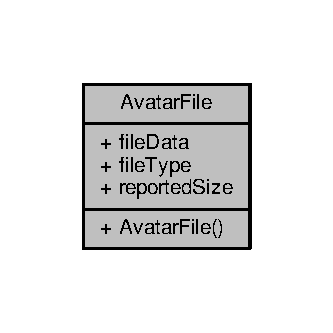
\includegraphics[width=160pt]{struct_avatar_file__coll__graph}
\end{center}
\end{figure}
\subsection*{Public 멤버 함수}
\begin{DoxyCompactItemize}
\item 
\hyperlink{struct_avatar_file_a737930aa86033509d0fd6f677512294f}{Avatar\-File} ()
\end{DoxyCompactItemize}
\subsection*{Public 속성}
\begin{DoxyCompactItemize}
\item 
std\-::vector$<$ unsigned char $>$ \hyperlink{struct_avatar_file_a6b38c3662255dfc8e33fba2188bb35b4}{file\-Data}
\item 
\hyperlink{playerdata_8h_a838468e0dd027767b891761d30d2bf39}{Avatar\-File\-Type} \hyperlink{struct_avatar_file_afd7760254880cef7bd1b464d0fea916b}{file\-Type}
\item 
size\-\_\-t \hyperlink{struct_avatar_file_a815e6f29eb421ab4732e6cd11245b4f8}{reported\-Size}
\end{DoxyCompactItemize}


\subsection{생성자 \& 소멸자 문서화}
\hypertarget{struct_avatar_file_a737930aa86033509d0fd6f677512294f}{\index{Avatar\-File@{Avatar\-File}!Avatar\-File@{Avatar\-File}}
\index{Avatar\-File@{Avatar\-File}!AvatarFile@{Avatar\-File}}
\subsubsection[{Avatar\-File}]{\setlength{\rightskip}{0pt plus 5cm}Avatar\-File\-::\-Avatar\-File (
\begin{DoxyParamCaption}
{}
\end{DoxyParamCaption}
)\hspace{0.3cm}{\ttfamily [inline]}}}\label{struct_avatar_file_a737930aa86033509d0fd6f677512294f}

\begin{DoxyCode}
66 : \hyperlink{struct_avatar_file_afd7760254880cef7bd1b464d0fea916b}{fileType}(\hyperlink{playerdata_8h_a838468e0dd027767b891761d30d2bf39af3195e1aaeb82da02f85ea7a293e91a1}{AVATAR\_FILE\_TYPE\_UNKNOWN}), 
      \hyperlink{struct_avatar_file_a815e6f29eb421ab4732e6cd11245b4f8}{reportedSize}(0) \{\}
\end{DoxyCode}


\subsection{멤버 데이타 문서화}
\hypertarget{struct_avatar_file_a6b38c3662255dfc8e33fba2188bb35b4}{\index{Avatar\-File@{Avatar\-File}!file\-Data@{file\-Data}}
\index{file\-Data@{file\-Data}!AvatarFile@{Avatar\-File}}
\subsubsection[{file\-Data}]{\setlength{\rightskip}{0pt plus 5cm}std\-::vector$<$unsigned char$>$ Avatar\-File\-::file\-Data}}\label{struct_avatar_file_a6b38c3662255dfc8e33fba2188bb35b4}
\hypertarget{struct_avatar_file_afd7760254880cef7bd1b464d0fea916b}{\index{Avatar\-File@{Avatar\-File}!file\-Type@{file\-Type}}
\index{file\-Type@{file\-Type}!AvatarFile@{Avatar\-File}}
\subsubsection[{file\-Type}]{\setlength{\rightskip}{0pt plus 5cm}{\bf Avatar\-File\-Type} Avatar\-File\-::file\-Type}}\label{struct_avatar_file_afd7760254880cef7bd1b464d0fea916b}
\hypertarget{struct_avatar_file_a815e6f29eb421ab4732e6cd11245b4f8}{\index{Avatar\-File@{Avatar\-File}!reported\-Size@{reported\-Size}}
\index{reported\-Size@{reported\-Size}!AvatarFile@{Avatar\-File}}
\subsubsection[{reported\-Size}]{\setlength{\rightskip}{0pt plus 5cm}size\-\_\-t Avatar\-File\-::reported\-Size}}\label{struct_avatar_file_a815e6f29eb421ab4732e6cd11245b4f8}


이 구조체에 대한 문서화 페이지는 다음의 파일로부터 생성되었습니다.\-:\begin{DoxyCompactItemize}
\item 
\hyperlink{playerdata_8h}{playerdata.\-h}\end{DoxyCompactItemize}

\hypertarget{struct_game_data}{\section{Game\-Data 구조체 참조}
\label{struct_game_data}\index{Game\-Data@{Game\-Data}}
}


{\ttfamily \#include $<$gamedata.\-h$>$}



Game\-Data에 대한 협력 다이어그램\-:\nopagebreak
\begin{figure}[H]
\begin{center}
\leavevmode
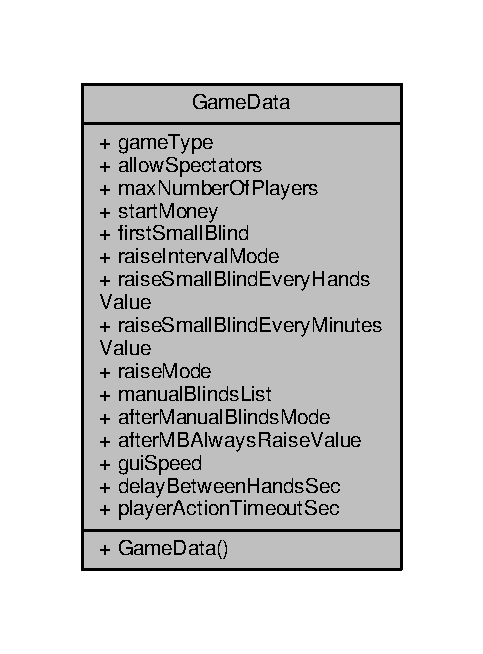
\includegraphics[width=232pt]{struct_game_data__coll__graph}
\end{center}
\end{figure}
\subsection*{Public 멤버 함수}
\begin{DoxyCompactItemize}
\item 
\hyperlink{struct_game_data_a67ab18c5a35df618e99983275c7552ab}{Game\-Data} ()
\end{DoxyCompactItemize}
\subsection*{Public 속성}
\begin{DoxyCompactItemize}
\item 
\hyperlink{gamedata_8h_a86864855734edb7b2cb1efdc7a03fd57}{Game\-Type} \hyperlink{struct_game_data_a44ded208d33fed8dbf1edd827faa847b}{game\-Type}
\item 
bool \hyperlink{struct_game_data_aa254390c51645ce5b18fd55e27e04f79}{allow\-Spectators}
\item 
int \hyperlink{struct_game_data_aba8c8d38c50dab71ad1530bbc2003b46}{max\-Number\-Of\-Players}
\item 
int \hyperlink{struct_game_data_a1b697f477ae03d3bd3323c4c099d6d58}{start\-Money}
\item 
int \hyperlink{struct_game_data_a0c9e8a63d5c02de30463c0b6beacebe3}{first\-Small\-Blind}
\item 
\hyperlink{gamedata_8h_a39f8de2f47cb4adf9038f5c6d6a8b8e6}{Raise\-Interval\-Mode} \hyperlink{struct_game_data_a298a24818a2bf81d8c7565812ff2eb26}{raise\-Interval\-Mode}
\item 
int \hyperlink{struct_game_data_a943a5365d2a5ac840bb3479c6fe1c23b}{raise\-Small\-Blind\-Every\-Hands\-Value}
\item 
int \hyperlink{struct_game_data_a6601463dbb7b1db927525b24d79e63b8}{raise\-Small\-Blind\-Every\-Minutes\-Value}
\item 
\hyperlink{gamedata_8h_a5532f34d7415bdfab60d67400cd5fc02}{Raise\-Mode} \hyperlink{struct_game_data_a592278fc8c3d824ddbdc3f8a401320bc}{raise\-Mode}
\item 
std\-::list$<$ int $>$ \hyperlink{struct_game_data_aff746a781ec8317d890f860ad450ab8e}{manual\-Blinds\-List}
\item 
\hyperlink{gamedata_8h_a250ebe9cdf4567798600e292202a66e6}{After\-Manual\-Blinds\-Mode} \hyperlink{struct_game_data_a7e8255dd232821d0419b31893b3acbb4}{after\-Manual\-Blinds\-Mode}
\item 
int \hyperlink{struct_game_data_a68e6f78103983935a5f6b20abb595355}{after\-M\-B\-Always\-Raise\-Value}
\item 
int \hyperlink{struct_game_data_a19b38d37fbd225504166856f187f38f3}{gui\-Speed}
\item 
int \hyperlink{struct_game_data_aa37d21f5ccbeca258400c07d7fbbf6da}{delay\-Between\-Hands\-Sec}
\item 
int \hyperlink{struct_game_data_a7379c03ecb75bda8cf95d215b41ae83b}{player\-Action\-Timeout\-Sec}
\end{DoxyCompactItemize}


\subsection{생성자 \& 소멸자 문서화}
\hypertarget{struct_game_data_a67ab18c5a35df618e99983275c7552ab}{\index{Game\-Data@{Game\-Data}!Game\-Data@{Game\-Data}}
\index{Game\-Data@{Game\-Data}!GameData@{Game\-Data}}
\subsubsection[{Game\-Data}]{\setlength{\rightskip}{0pt plus 5cm}Game\-Data\-::\-Game\-Data (
\begin{DoxyParamCaption}
{}
\end{DoxyParamCaption}
)\hspace{0.3cm}{\ttfamily [inline]}}}\label{struct_game_data_a67ab18c5a35df618e99983275c7552ab}

\begin{DoxyCode}
75                : \hyperlink{struct_game_data_a44ded208d33fed8dbf1edd827faa847b}{gameType}(\hyperlink{gamedata_8h_a86864855734edb7b2cb1efdc7a03fd57a9b38699b42326665c8f890f41974dc79}{GAME\_TYPE\_NORMAL}), 
      \hyperlink{struct_game_data_aa254390c51645ce5b18fd55e27e04f79}{allowSpectators}(\textcolor{keyword}{true}),
76         \hyperlink{struct_game_data_aba8c8d38c50dab71ad1530bbc2003b46}{maxNumberOfPlayers}(0), \hyperlink{struct_game_data_a1b697f477ae03d3bd3323c4c099d6d58}{startMoney}(0), 
      \hyperlink{struct_game_data_a0c9e8a63d5c02de30463c0b6beacebe3}{firstSmallBlind}(0),
77         \hyperlink{struct_game_data_a298a24818a2bf81d8c7565812ff2eb26}{raiseIntervalMode}(\hyperlink{gamedata_8h_a39f8de2f47cb4adf9038f5c6d6a8b8e6a27cf82917dfcb27e20ee920f1158aff4}{RAISE\_ON\_HANDNUMBER}), 
      \hyperlink{struct_game_data_a943a5365d2a5ac840bb3479c6fe1c23b}{raiseSmallBlindEveryHandsValue}(8),
78         \hyperlink{struct_game_data_a6601463dbb7b1db927525b24d79e63b8}{raiseSmallBlindEveryMinutesValue}(1), 
      \hyperlink{struct_game_data_a592278fc8c3d824ddbdc3f8a401320bc}{raiseMode}(\hyperlink{gamedata_8h_a5532f34d7415bdfab60d67400cd5fc02aec798914fb0781d6838679ab06926a56}{DOUBLE\_BLINDS}),
79         \hyperlink{struct_game_data_a7e8255dd232821d0419b31893b3acbb4}{afterManualBlindsMode}(\hyperlink{gamedata_8h_a250ebe9cdf4567798600e292202a66e6ac0e8cd440d7884b189fdb2e1a46aeebb}{AFTERMB\_DOUBLE\_BLINDS}), 
      \hyperlink{struct_game_data_a68e6f78103983935a5f6b20abb595355}{afterMBAlwaysRaiseValue}(0),
80         \hyperlink{struct_game_data_a19b38d37fbd225504166856f187f38f3}{guiSpeed}(4), \hyperlink{struct_game_data_aa37d21f5ccbeca258400c07d7fbbf6da}{delayBetweenHandsSec}(6), 
      \hyperlink{struct_game_data_a7379c03ecb75bda8cf95d215b41ae83b}{playerActionTimeoutSec}(20) \{\}
\end{DoxyCode}


\subsection{멤버 데이타 문서화}
\hypertarget{struct_game_data_a7e8255dd232821d0419b31893b3acbb4}{\index{Game\-Data@{Game\-Data}!after\-Manual\-Blinds\-Mode@{after\-Manual\-Blinds\-Mode}}
\index{after\-Manual\-Blinds\-Mode@{after\-Manual\-Blinds\-Mode}!GameData@{Game\-Data}}
\subsubsection[{after\-Manual\-Blinds\-Mode}]{\setlength{\rightskip}{0pt plus 5cm}{\bf After\-Manual\-Blinds\-Mode} Game\-Data\-::after\-Manual\-Blinds\-Mode}}\label{struct_game_data_a7e8255dd232821d0419b31893b3acbb4}
\hypertarget{struct_game_data_a68e6f78103983935a5f6b20abb595355}{\index{Game\-Data@{Game\-Data}!after\-M\-B\-Always\-Raise\-Value@{after\-M\-B\-Always\-Raise\-Value}}
\index{after\-M\-B\-Always\-Raise\-Value@{after\-M\-B\-Always\-Raise\-Value}!GameData@{Game\-Data}}
\subsubsection[{after\-M\-B\-Always\-Raise\-Value}]{\setlength{\rightskip}{0pt plus 5cm}int Game\-Data\-::after\-M\-B\-Always\-Raise\-Value}}\label{struct_game_data_a68e6f78103983935a5f6b20abb595355}
\hypertarget{struct_game_data_aa254390c51645ce5b18fd55e27e04f79}{\index{Game\-Data@{Game\-Data}!allow\-Spectators@{allow\-Spectators}}
\index{allow\-Spectators@{allow\-Spectators}!GameData@{Game\-Data}}
\subsubsection[{allow\-Spectators}]{\setlength{\rightskip}{0pt plus 5cm}bool Game\-Data\-::allow\-Spectators}}\label{struct_game_data_aa254390c51645ce5b18fd55e27e04f79}
\hypertarget{struct_game_data_aa37d21f5ccbeca258400c07d7fbbf6da}{\index{Game\-Data@{Game\-Data}!delay\-Between\-Hands\-Sec@{delay\-Between\-Hands\-Sec}}
\index{delay\-Between\-Hands\-Sec@{delay\-Between\-Hands\-Sec}!GameData@{Game\-Data}}
\subsubsection[{delay\-Between\-Hands\-Sec}]{\setlength{\rightskip}{0pt plus 5cm}int Game\-Data\-::delay\-Between\-Hands\-Sec}}\label{struct_game_data_aa37d21f5ccbeca258400c07d7fbbf6da}
\hypertarget{struct_game_data_a0c9e8a63d5c02de30463c0b6beacebe3}{\index{Game\-Data@{Game\-Data}!first\-Small\-Blind@{first\-Small\-Blind}}
\index{first\-Small\-Blind@{first\-Small\-Blind}!GameData@{Game\-Data}}
\subsubsection[{first\-Small\-Blind}]{\setlength{\rightskip}{0pt plus 5cm}int Game\-Data\-::first\-Small\-Blind}}\label{struct_game_data_a0c9e8a63d5c02de30463c0b6beacebe3}
\hypertarget{struct_game_data_a44ded208d33fed8dbf1edd827faa847b}{\index{Game\-Data@{Game\-Data}!game\-Type@{game\-Type}}
\index{game\-Type@{game\-Type}!GameData@{Game\-Data}}
\subsubsection[{game\-Type}]{\setlength{\rightskip}{0pt plus 5cm}{\bf Game\-Type} Game\-Data\-::game\-Type}}\label{struct_game_data_a44ded208d33fed8dbf1edd827faa847b}
\hypertarget{struct_game_data_a19b38d37fbd225504166856f187f38f3}{\index{Game\-Data@{Game\-Data}!gui\-Speed@{gui\-Speed}}
\index{gui\-Speed@{gui\-Speed}!GameData@{Game\-Data}}
\subsubsection[{gui\-Speed}]{\setlength{\rightskip}{0pt plus 5cm}int Game\-Data\-::gui\-Speed}}\label{struct_game_data_a19b38d37fbd225504166856f187f38f3}
\hypertarget{struct_game_data_aff746a781ec8317d890f860ad450ab8e}{\index{Game\-Data@{Game\-Data}!manual\-Blinds\-List@{manual\-Blinds\-List}}
\index{manual\-Blinds\-List@{manual\-Blinds\-List}!GameData@{Game\-Data}}
\subsubsection[{manual\-Blinds\-List}]{\setlength{\rightskip}{0pt plus 5cm}std\-::list$<$int$>$ Game\-Data\-::manual\-Blinds\-List}}\label{struct_game_data_aff746a781ec8317d890f860ad450ab8e}
\hypertarget{struct_game_data_aba8c8d38c50dab71ad1530bbc2003b46}{\index{Game\-Data@{Game\-Data}!max\-Number\-Of\-Players@{max\-Number\-Of\-Players}}
\index{max\-Number\-Of\-Players@{max\-Number\-Of\-Players}!GameData@{Game\-Data}}
\subsubsection[{max\-Number\-Of\-Players}]{\setlength{\rightskip}{0pt plus 5cm}int Game\-Data\-::max\-Number\-Of\-Players}}\label{struct_game_data_aba8c8d38c50dab71ad1530bbc2003b46}
\hypertarget{struct_game_data_a7379c03ecb75bda8cf95d215b41ae83b}{\index{Game\-Data@{Game\-Data}!player\-Action\-Timeout\-Sec@{player\-Action\-Timeout\-Sec}}
\index{player\-Action\-Timeout\-Sec@{player\-Action\-Timeout\-Sec}!GameData@{Game\-Data}}
\subsubsection[{player\-Action\-Timeout\-Sec}]{\setlength{\rightskip}{0pt plus 5cm}int Game\-Data\-::player\-Action\-Timeout\-Sec}}\label{struct_game_data_a7379c03ecb75bda8cf95d215b41ae83b}
\hypertarget{struct_game_data_a298a24818a2bf81d8c7565812ff2eb26}{\index{Game\-Data@{Game\-Data}!raise\-Interval\-Mode@{raise\-Interval\-Mode}}
\index{raise\-Interval\-Mode@{raise\-Interval\-Mode}!GameData@{Game\-Data}}
\subsubsection[{raise\-Interval\-Mode}]{\setlength{\rightskip}{0pt plus 5cm}{\bf Raise\-Interval\-Mode} Game\-Data\-::raise\-Interval\-Mode}}\label{struct_game_data_a298a24818a2bf81d8c7565812ff2eb26}
\hypertarget{struct_game_data_a592278fc8c3d824ddbdc3f8a401320bc}{\index{Game\-Data@{Game\-Data}!raise\-Mode@{raise\-Mode}}
\index{raise\-Mode@{raise\-Mode}!GameData@{Game\-Data}}
\subsubsection[{raise\-Mode}]{\setlength{\rightskip}{0pt plus 5cm}{\bf Raise\-Mode} Game\-Data\-::raise\-Mode}}\label{struct_game_data_a592278fc8c3d824ddbdc3f8a401320bc}
\hypertarget{struct_game_data_a943a5365d2a5ac840bb3479c6fe1c23b}{\index{Game\-Data@{Game\-Data}!raise\-Small\-Blind\-Every\-Hands\-Value@{raise\-Small\-Blind\-Every\-Hands\-Value}}
\index{raise\-Small\-Blind\-Every\-Hands\-Value@{raise\-Small\-Blind\-Every\-Hands\-Value}!GameData@{Game\-Data}}
\subsubsection[{raise\-Small\-Blind\-Every\-Hands\-Value}]{\setlength{\rightskip}{0pt plus 5cm}int Game\-Data\-::raise\-Small\-Blind\-Every\-Hands\-Value}}\label{struct_game_data_a943a5365d2a5ac840bb3479c6fe1c23b}
\hypertarget{struct_game_data_a6601463dbb7b1db927525b24d79e63b8}{\index{Game\-Data@{Game\-Data}!raise\-Small\-Blind\-Every\-Minutes\-Value@{raise\-Small\-Blind\-Every\-Minutes\-Value}}
\index{raise\-Small\-Blind\-Every\-Minutes\-Value@{raise\-Small\-Blind\-Every\-Minutes\-Value}!GameData@{Game\-Data}}
\subsubsection[{raise\-Small\-Blind\-Every\-Minutes\-Value}]{\setlength{\rightskip}{0pt plus 5cm}int Game\-Data\-::raise\-Small\-Blind\-Every\-Minutes\-Value}}\label{struct_game_data_a6601463dbb7b1db927525b24d79e63b8}
\hypertarget{struct_game_data_a1b697f477ae03d3bd3323c4c099d6d58}{\index{Game\-Data@{Game\-Data}!start\-Money@{start\-Money}}
\index{start\-Money@{start\-Money}!GameData@{Game\-Data}}
\subsubsection[{start\-Money}]{\setlength{\rightskip}{0pt plus 5cm}int Game\-Data\-::start\-Money}}\label{struct_game_data_a1b697f477ae03d3bd3323c4c099d6d58}


이 구조체에 대한 문서화 페이지는 다음의 파일로부터 생성되었습니다.\-:\begin{DoxyCompactItemize}
\item 
\hyperlink{gamedata_8h}{gamedata.\-h}\end{DoxyCompactItemize}

\hypertarget{struct_game_info}{\section{Game\-Info 구조체 참조}
\label{struct_game_info}\index{Game\-Info@{Game\-Info}}
}


{\ttfamily \#include $<$gamedata.\-h$>$}



Game\-Info에 대한 협력 다이어그램\-:\nopagebreak
\begin{figure}[H]
\begin{center}
\leavevmode
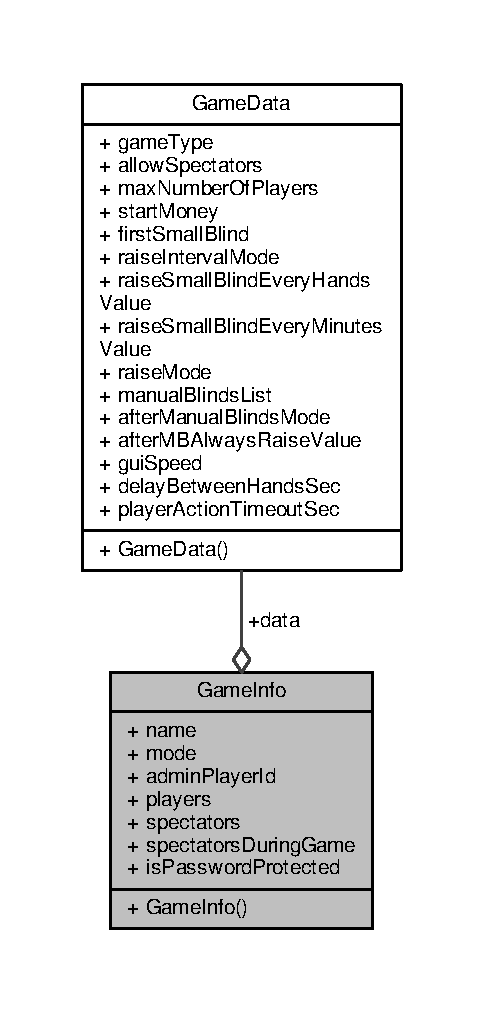
\includegraphics[width=232pt]{struct_game_info__coll__graph}
\end{center}
\end{figure}
\subsection*{Public 멤버 함수}
\begin{DoxyCompactItemize}
\item 
\hyperlink{struct_game_info_ae7ded63bd69b007847bd66debaeebc23}{Game\-Info} ()
\end{DoxyCompactItemize}
\subsection*{Public 속성}
\begin{DoxyCompactItemize}
\item 
std\-::string \hyperlink{struct_game_info_a2636537f5709e2f0a492e21f46d63902}{name}
\item 
\hyperlink{struct_game_data}{Game\-Data} \hyperlink{struct_game_info_adda7dce486bafa025f007cc38fb5ff4c}{data}
\item 
\hyperlink{gamedata_8h_aaf5ef5a17b53e9997c837b07015589de}{Game\-Mode} \hyperlink{struct_game_info_a22140503539e3356bf8b19b041ccf934}{mode}
\item 
unsigned \hyperlink{struct_game_info_a5ecc1639834e9a6f8055f38c1f18c2d9}{admin\-Player\-Id}
\item 
\hyperlink{gamedata_8h_a02ee63ca030dfa9d119c9f2df584e383}{Player\-Id\-List} \hyperlink{struct_game_info_abae703a83db0cab47682304c2f5175bf}{players}
\item 
\hyperlink{gamedata_8h_a02ee63ca030dfa9d119c9f2df584e383}{Player\-Id\-List} \hyperlink{struct_game_info_a512e7504e87265d990be1fc6d6a3b07e}{spectators}
\item 
\hyperlink{gamedata_8h_a02ee63ca030dfa9d119c9f2df584e383}{Player\-Id\-List} \hyperlink{struct_game_info_a24be82c5206c45ff9f08fa9896783332}{spectators\-During\-Game}
\item 
bool \hyperlink{struct_game_info_a0d282d0891f202cffd9f2b4d55721123}{is\-Password\-Protected}
\end{DoxyCompactItemize}


\subsection{생성자 \& 소멸자 문서화}
\hypertarget{struct_game_info_ae7ded63bd69b007847bd66debaeebc23}{\index{Game\-Info@{Game\-Info}!Game\-Info@{Game\-Info}}
\index{Game\-Info@{Game\-Info}!GameInfo@{Game\-Info}}
\subsubsection[{Game\-Info}]{\setlength{\rightskip}{0pt plus 5cm}Game\-Info\-::\-Game\-Info (
\begin{DoxyParamCaption}
{}
\end{DoxyParamCaption}
)\hspace{0.3cm}{\ttfamily [inline]}}}\label{struct_game_info_ae7ded63bd69b007847bd66debaeebc23}

\begin{DoxyCode}
99 : \hyperlink{struct_game_info_a22140503539e3356bf8b19b041ccf934}{mode}(\hyperlink{gamedata_8h_aaf5ef5a17b53e9997c837b07015589dea5189be813705a7ad4b236a347c394328}{GAME\_MODE\_CREATED}), \hyperlink{struct_game_info_a5ecc1639834e9a6f8055f38c1f18c2d9}{adminPlayerId}(0), 
      \hyperlink{struct_game_info_a0d282d0891f202cffd9f2b4d55721123}{isPasswordProtected}(\textcolor{keyword}{false}) \{\}
\end{DoxyCode}


\subsection{멤버 데이타 문서화}
\hypertarget{struct_game_info_a5ecc1639834e9a6f8055f38c1f18c2d9}{\index{Game\-Info@{Game\-Info}!admin\-Player\-Id@{admin\-Player\-Id}}
\index{admin\-Player\-Id@{admin\-Player\-Id}!GameInfo@{Game\-Info}}
\subsubsection[{admin\-Player\-Id}]{\setlength{\rightskip}{0pt plus 5cm}unsigned Game\-Info\-::admin\-Player\-Id}}\label{struct_game_info_a5ecc1639834e9a6f8055f38c1f18c2d9}
\hypertarget{struct_game_info_adda7dce486bafa025f007cc38fb5ff4c}{\index{Game\-Info@{Game\-Info}!data@{data}}
\index{data@{data}!GameInfo@{Game\-Info}}
\subsubsection[{data}]{\setlength{\rightskip}{0pt plus 5cm}{\bf Game\-Data} Game\-Info\-::data}}\label{struct_game_info_adda7dce486bafa025f007cc38fb5ff4c}
\hypertarget{struct_game_info_a0d282d0891f202cffd9f2b4d55721123}{\index{Game\-Info@{Game\-Info}!is\-Password\-Protected@{is\-Password\-Protected}}
\index{is\-Password\-Protected@{is\-Password\-Protected}!GameInfo@{Game\-Info}}
\subsubsection[{is\-Password\-Protected}]{\setlength{\rightskip}{0pt plus 5cm}bool Game\-Info\-::is\-Password\-Protected}}\label{struct_game_info_a0d282d0891f202cffd9f2b4d55721123}
\hypertarget{struct_game_info_a22140503539e3356bf8b19b041ccf934}{\index{Game\-Info@{Game\-Info}!mode@{mode}}
\index{mode@{mode}!GameInfo@{Game\-Info}}
\subsubsection[{mode}]{\setlength{\rightskip}{0pt plus 5cm}{\bf Game\-Mode} Game\-Info\-::mode}}\label{struct_game_info_a22140503539e3356bf8b19b041ccf934}
\hypertarget{struct_game_info_a2636537f5709e2f0a492e21f46d63902}{\index{Game\-Info@{Game\-Info}!name@{name}}
\index{name@{name}!GameInfo@{Game\-Info}}
\subsubsection[{name}]{\setlength{\rightskip}{0pt plus 5cm}std\-::string Game\-Info\-::name}}\label{struct_game_info_a2636537f5709e2f0a492e21f46d63902}
\hypertarget{struct_game_info_abae703a83db0cab47682304c2f5175bf}{\index{Game\-Info@{Game\-Info}!players@{players}}
\index{players@{players}!GameInfo@{Game\-Info}}
\subsubsection[{players}]{\setlength{\rightskip}{0pt plus 5cm}{\bf Player\-Id\-List} Game\-Info\-::players}}\label{struct_game_info_abae703a83db0cab47682304c2f5175bf}
\hypertarget{struct_game_info_a512e7504e87265d990be1fc6d6a3b07e}{\index{Game\-Info@{Game\-Info}!spectators@{spectators}}
\index{spectators@{spectators}!GameInfo@{Game\-Info}}
\subsubsection[{spectators}]{\setlength{\rightskip}{0pt plus 5cm}{\bf Player\-Id\-List} Game\-Info\-::spectators}}\label{struct_game_info_a512e7504e87265d990be1fc6d6a3b07e}
\hypertarget{struct_game_info_a24be82c5206c45ff9f08fa9896783332}{\index{Game\-Info@{Game\-Info}!spectators\-During\-Game@{spectators\-During\-Game}}
\index{spectators\-During\-Game@{spectators\-During\-Game}!GameInfo@{Game\-Info}}
\subsubsection[{spectators\-During\-Game}]{\setlength{\rightskip}{0pt plus 5cm}{\bf Player\-Id\-List} Game\-Info\-::spectators\-During\-Game}}\label{struct_game_info_a24be82c5206c45ff9f08fa9896783332}


이 구조체에 대한 문서화 페이지는 다음의 파일로부터 생성되었습니다.\-:\begin{DoxyCompactItemize}
\item 
\hyperlink{gamedata_8h}{gamedata.\-h}\end{DoxyCompactItemize}

\hypertarget{struct_net_session}{\section{Net\-Session 구조체 참조}
\label{struct_net_session}\index{Net\-Session@{Net\-Session}}
}


Net\-Session에 대한 협력 다이어그램\-:\nopagebreak
\begin{figure}[H]
\begin{center}
\leavevmode
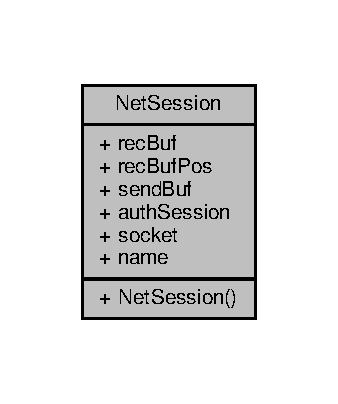
\includegraphics[width=162pt]{struct_net_session__coll__graph}
\end{center}
\end{figure}
\subsection*{Public 멤버 함수}
\begin{DoxyCompactItemize}
\item 
\hyperlink{struct_net_session_a636704de0a367698b2ec93e65b21a300}{Net\-Session} (boost\-::asio\-::io\-\_\-service \&io\-Service)
\end{DoxyCompactItemize}
\subsection*{Public 속성}
\begin{DoxyCompactItemize}
\item 
boost\-::array$<$ char, \hyperlink{load_8cpp_a6821bafc3c88dfb2e433a095df9940c6}{B\-U\-F\-\_\-\-S\-I\-Z\-E} $>$ \hyperlink{struct_net_session_ae53e0baac8f14adba2d5b7d71c715ce7}{rec\-Buf}
\item 
size\-\_\-t \hyperlink{struct_net_session_abf9c78874e44c3aa6176e288e77f5aae}{rec\-Buf\-Pos}
\item 
boost\-::array$<$ char, \hyperlink{load_8cpp_a6821bafc3c88dfb2e433a095df9940c6}{B\-U\-F\-\_\-\-S\-I\-Z\-E} $>$ \hyperlink{struct_net_session_a6e3c17623ebe78851968a210e95fcc38}{send\-Buf}
\item 
Gsasl\-\_\-session $\ast$ \hyperlink{struct_net_session_a633af90850d032509cfa243abb6898a8}{auth\-Session}
\item 
tcp\-::socket \hyperlink{struct_net_session_a93ead5e6efef575fd61ed0514100310b}{socket}
\item 
string \hyperlink{struct_net_session_aec0bfb7bd042d9f19df3fc91dd8accae}{name}
\end{DoxyCompactItemize}


\subsection{생성자 \& 소멸자 문서화}
\hypertarget{struct_net_session_a636704de0a367698b2ec93e65b21a300}{\index{Net\-Session@{Net\-Session}!Net\-Session@{Net\-Session}}
\index{Net\-Session@{Net\-Session}!NetSession@{Net\-Session}}
\subsubsection[{Net\-Session}]{\setlength{\rightskip}{0pt plus 5cm}Net\-Session\-::\-Net\-Session (
\begin{DoxyParamCaption}
\item[{boost\-::asio\-::io\-\_\-service \&}]{io\-Service}
\end{DoxyParamCaption}
)\hspace{0.3cm}{\ttfamily [inline]}}}\label{struct_net_session_a636704de0a367698b2ec93e65b21a300}

\begin{DoxyCode}
53 : \hyperlink{struct_net_session_abf9c78874e44c3aa6176e288e77f5aae}{recBufPos}(0), \hyperlink{struct_net_session_a633af90850d032509cfa243abb6898a8}{authSession}(NULL), \hyperlink{struct_net_session_a93ead5e6efef575fd61ed0514100310b}{socket}(ioService) \{\}
\end{DoxyCode}


\subsection{멤버 데이타 문서화}
\hypertarget{struct_net_session_a633af90850d032509cfa243abb6898a8}{\index{Net\-Session@{Net\-Session}!auth\-Session@{auth\-Session}}
\index{auth\-Session@{auth\-Session}!NetSession@{Net\-Session}}
\subsubsection[{auth\-Session}]{\setlength{\rightskip}{0pt plus 5cm}Gsasl\-\_\-session$\ast$ Net\-Session\-::auth\-Session}}\label{struct_net_session_a633af90850d032509cfa243abb6898a8}
\hypertarget{struct_net_session_aec0bfb7bd042d9f19df3fc91dd8accae}{\index{Net\-Session@{Net\-Session}!name@{name}}
\index{name@{name}!NetSession@{Net\-Session}}
\subsubsection[{name}]{\setlength{\rightskip}{0pt plus 5cm}string Net\-Session\-::name}}\label{struct_net_session_aec0bfb7bd042d9f19df3fc91dd8accae}
\hypertarget{struct_net_session_ae53e0baac8f14adba2d5b7d71c715ce7}{\index{Net\-Session@{Net\-Session}!rec\-Buf@{rec\-Buf}}
\index{rec\-Buf@{rec\-Buf}!NetSession@{Net\-Session}}
\subsubsection[{rec\-Buf}]{\setlength{\rightskip}{0pt plus 5cm}boost\-::array$<$char, {\bf B\-U\-F\-\_\-\-S\-I\-Z\-E}$>$ Net\-Session\-::rec\-Buf}}\label{struct_net_session_ae53e0baac8f14adba2d5b7d71c715ce7}
\hypertarget{struct_net_session_abf9c78874e44c3aa6176e288e77f5aae}{\index{Net\-Session@{Net\-Session}!rec\-Buf\-Pos@{rec\-Buf\-Pos}}
\index{rec\-Buf\-Pos@{rec\-Buf\-Pos}!NetSession@{Net\-Session}}
\subsubsection[{rec\-Buf\-Pos}]{\setlength{\rightskip}{0pt plus 5cm}size\-\_\-t Net\-Session\-::rec\-Buf\-Pos}}\label{struct_net_session_abf9c78874e44c3aa6176e288e77f5aae}
\hypertarget{struct_net_session_a6e3c17623ebe78851968a210e95fcc38}{\index{Net\-Session@{Net\-Session}!send\-Buf@{send\-Buf}}
\index{send\-Buf@{send\-Buf}!NetSession@{Net\-Session}}
\subsubsection[{send\-Buf}]{\setlength{\rightskip}{0pt plus 5cm}boost\-::array$<$char, {\bf B\-U\-F\-\_\-\-S\-I\-Z\-E}$>$ Net\-Session\-::send\-Buf}}\label{struct_net_session_a6e3c17623ebe78851968a210e95fcc38}
\hypertarget{struct_net_session_a93ead5e6efef575fd61ed0514100310b}{\index{Net\-Session@{Net\-Session}!socket@{socket}}
\index{socket@{socket}!NetSession@{Net\-Session}}
\subsubsection[{socket}]{\setlength{\rightskip}{0pt plus 5cm}tcp\-::socket Net\-Session\-::socket}}\label{struct_net_session_a93ead5e6efef575fd61ed0514100310b}


이 구조체에 대한 문서화 페이지는 다음의 파일로부터 생성되었습니다.\-:\begin{DoxyCompactItemize}
\item 
\hyperlink{load_8cpp}{load.\-cpp}\end{DoxyCompactItemize}

\hypertarget{class_player_data}{\section{Player\-Data 클래스 참조}
\label{class_player_data}\index{Player\-Data@{Player\-Data}}
}


{\ttfamily \#include $<$playerdata.\-h$>$}



Player\-Data에 대한 협력 다이어그램\-:
\nopagebreak
\begin{figure}[H]
\begin{center}
\leavevmode
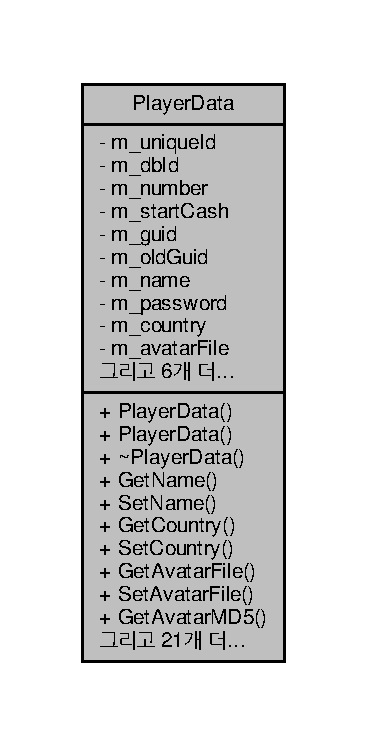
\includegraphics[width=176pt]{class_player_data__coll__graph}
\end{center}
\end{figure}
\subsection*{Public 멤버 함수}
\begin{DoxyCompactItemize}
\item 
\hyperlink{class_player_data_afd58f88036497dea0cd37e01fe14de5b}{Player\-Data} (unsigned unique\-Id, int number, \hyperlink{playerdata_8h_abe590f3c9109f404f003d5d7e4f0fccf}{Player\-Type} type, \hyperlink{playerdata_8h_ac0c72aca5c5ceabb2abbcd2d2c02aba6}{Player\-Rights} rights, bool is\-Game\-Admin)
\item 
\hyperlink{class_player_data_a7d58f6cfbdbdc4e9066772dc57e5c9dc}{Player\-Data} (const \hyperlink{class_player_data}{Player\-Data} \&other)
\item 
\hyperlink{class_player_data_a253ae40fb805d8ff0cf9d884ab504d8a}{$\sim$\-Player\-Data} ()
\item 
std\-::string \hyperlink{class_player_data_a9ccadf260a63a25c0a2644a9863dba45}{Get\-Name} () const 
\item 
void \hyperlink{class_player_data_a0ce3965e0a0baf505eca8e13d7580f19}{Set\-Name} (const std\-::string \&name)
\item 
std\-::string \hyperlink{class_player_data_a613727a01585bb57e61dfc88813b8e56}{Get\-Country} () const 
\item 
void \hyperlink{class_player_data_aeb99c2c6ed25af7cfd46849bef370f4f}{Set\-Country} (const std\-::string \&country)
\item 
std\-::string \hyperlink{class_player_data_a8a0cf1e986ececc7491e989e557a3383}{Get\-Avatar\-File} () const 
\item 
void \hyperlink{class_player_data_a8174f11d0740db3f312c6b13fb2fe737}{Set\-Avatar\-File} (const std\-::string \&avatar\-File)
\item 
M\-D5\-Buf \hyperlink{class_player_data_aa305d3aced0a792551cebf1ea6a3eafa}{Get\-Avatar\-M\-D5} () const 
\item 
void \hyperlink{class_player_data_a57ed0efa276e6a62add8cf6ae0f1e54f}{Set\-Avatar\-M\-D5} (const M\-D5\-Buf \&avatar\-M\-D5)
\item 
boost\-::shared\-\_\-ptr$<$ \hyperlink{struct_avatar_file}{Avatar\-File} $>$ \hyperlink{class_player_data_acbe5b0799bf0eeb1ba462bf38f3a66a8}{Get\-Net\-Avatar\-File} () const 
\item 
void \hyperlink{class_player_data_ac3d0ad92de2c8e42f7df88b40e75003d}{Set\-Net\-Avatar\-File} (boost\-::shared\-\_\-ptr$<$ \hyperlink{struct_avatar_file}{Avatar\-File} $>$ \hyperlink{struct_avatar_file}{Avatar\-File})
\item 
\hyperlink{playerdata_8h_abe590f3c9109f404f003d5d7e4f0fccf}{Player\-Type} \hyperlink{class_player_data_abfb06f847beee982e86ad29d03edc3b5}{Get\-Type} () const 
\item 
void \hyperlink{class_player_data_a8a32bc6cc032cccbab4d761054f8578a}{Set\-Type} (\hyperlink{playerdata_8h_abe590f3c9109f404f003d5d7e4f0fccf}{Player\-Type} type)
\item 
\hyperlink{playerdata_8h_ac0c72aca5c5ceabb2abbcd2d2c02aba6}{Player\-Rights} \hyperlink{class_player_data_a6ec702f92553198aabca8a235dc2b995}{Get\-Rights} () const 
\item 
void \hyperlink{class_player_data_a6496cec308484ed8f3ef100721d6461d}{Set\-Rights} (\hyperlink{playerdata_8h_ac0c72aca5c5ceabb2abbcd2d2c02aba6}{Player\-Rights} rights)
\item 
bool \hyperlink{class_player_data_a0203b2a5c2042d46f0ca838c94db88fc}{Is\-Game\-Admin} () const 
\item 
void \hyperlink{class_player_data_a926cfc7ff5a727ae5c0e072f0a1e947e}{Set\-Game\-Admin} (bool is\-Admin)
\item 
unsigned \hyperlink{class_player_data_a9922629a2ab29426703454a3b1554e38}{Get\-Unique\-Id} () const 
\item 
int \hyperlink{class_player_data_a0597b5d7c731ad08862eff9f5fb48754}{Get\-Number} () const 
\item 
void \hyperlink{class_player_data_acc626969fae365d9a85134c1602620de}{Set\-Number} (int number)
\item 
std\-::string \hyperlink{class_player_data_a84d85d3024a526f9887bf50e20c504e4}{Get\-Guid} () const 
\item 
void \hyperlink{class_player_data_ae6df82d891bb33d3d6ebe7e42d9bff07}{Set\-Guid} (const std\-::string \&guid)
\item 
std\-::string \hyperlink{class_player_data_af3ec6bf093ef6ba0d2bc1497907d8c6c}{Get\-Old\-Guid} () const 
\item 
void \hyperlink{class_player_data_a575e319875bdd901034d54be2f88ea12}{Set\-Old\-Guid} (const std\-::string \&guid)
\item 
D\-B\-\_\-id \hyperlink{class_player_data_a574ecee71638104326860bfa4438dcf5}{Get\-D\-B\-Id} () const 
\item 
void \hyperlink{class_player_data_a0f20856a42691cc4f917763307f895e0}{Set\-D\-B\-Id} (D\-B\-\_\-id id)
\item 
int \hyperlink{class_player_data_a54eab50fb80ec7f18ce1777c3632a73d}{Get\-Start\-Cash} () const 
\item 
void \hyperlink{class_player_data_ab0b58b77fb2366c31ff902cd91117919}{Set\-Start\-Cash} (int cash)
\item 
bool \hyperlink{class_player_data_afa03422cfe10bf02083f65746e2fb723}{operator$<$} (const \hyperlink{class_player_data}{Player\-Data} \&other) const 
\end{DoxyCompactItemize}
\subsection*{Private 속성}
\begin{DoxyCompactItemize}
\item 
const unsigned \hyperlink{class_player_data_a2b6ed5c114b242c39eab3ec7c6622a5f}{m\-\_\-unique\-Id}
\item 
D\-B\-\_\-id \hyperlink{class_player_data_af4a330231d9309b6e703f4c4fda251a8}{m\-\_\-db\-Id}
\item 
int \hyperlink{class_player_data_a00807837606a10faee2849b979181402}{m\-\_\-number}
\item 
int \hyperlink{class_player_data_afb53d1b4126139cdc74b8322dab0094a}{m\-\_\-start\-Cash}
\item 
std\-::string \hyperlink{class_player_data_a3d3abd9ce7a8421596ce2ec2bf16bd64}{m\-\_\-guid}
\item 
std\-::string \hyperlink{class_player_data_aac3ac77674157db291a3f49076bcb4bc}{m\-\_\-old\-Guid}
\item 
std\-::string \hyperlink{class_player_data_a0174f971f59af5008301ac6eb3d2304c}{m\-\_\-name}
\item 
std\-::string \hyperlink{class_player_data_a2cbffcef76225936b3860adcd0ab6e03}{m\-\_\-password}
\item 
std\-::string \hyperlink{class_player_data_af349fdb550aaac72ccaead9a156be844}{m\-\_\-country}
\item 
std\-::string \hyperlink{class_player_data_aa3342ab34d521ab87edd40ec7622be56}{m\-\_\-avatar\-File}
\item 
M\-D5\-Buf \hyperlink{class_player_data_a5a6b19ae010990245ed6214be517f2cf}{m\-\_\-avatar\-M\-D5}
\item 
\hyperlink{playerdata_8h_abe590f3c9109f404f003d5d7e4f0fccf}{Player\-Type} \hyperlink{class_player_data_a3e4b8d9fcda3d2def5f0a79468a87903}{m\-\_\-type}
\item 
\hyperlink{playerdata_8h_ac0c72aca5c5ceabb2abbcd2d2c02aba6}{Player\-Rights} \hyperlink{class_player_data_aa764ce6a7e503e938865f52463c48d63}{m\-\_\-rights}
\item 
bool \hyperlink{class_player_data_ad7c207bf8ecc38e2f86bdd8d83c935df}{m\-\_\-is\-Game\-Admin}
\item 
boost\-::shared\-\_\-ptr$<$ \hyperlink{struct_avatar_file}{Avatar\-File} $>$ \hyperlink{class_player_data_afafb202de188ebee15e54b49aa96feac}{m\-\_\-net\-Avatar\-File}
\item 
boost\-::mutex \hyperlink{class_player_data_a8e1276aab88bec3fa48e3c59f193827e}{m\-\_\-data\-Mutex}
\end{DoxyCompactItemize}


\subsection{생성자 \& 소멸자 문서화}
\hypertarget{class_player_data_afd58f88036497dea0cd37e01fe14de5b}{\index{Player\-Data@{Player\-Data}!Player\-Data@{Player\-Data}}
\index{Player\-Data@{Player\-Data}!PlayerData@{Player\-Data}}
\subsubsection[{Player\-Data}]{\setlength{\rightskip}{0pt plus 5cm}Player\-Data\-::\-Player\-Data (
\begin{DoxyParamCaption}
\item[{unsigned}]{unique\-Id, }
\item[{int}]{number, }
\item[{{\bf Player\-Type}}]{type, }
\item[{{\bf Player\-Rights}}]{rights, }
\item[{bool}]{is\-Game\-Admin}
\end{DoxyParamCaption}
)}}\label{class_player_data_afd58f88036497dea0cd37e01fe14de5b}

\begin{DoxyCode}
36     : \hyperlink{class_player_data_a2b6ed5c114b242c39eab3ec7c6622a5f}{m\_uniqueId}(uniqueId), \hyperlink{class_player_data_af4a330231d9309b6e703f4c4fda251a8}{m\_dbId}(DB\_ID\_INVALID), \hyperlink{class_player_data_a00807837606a10faee2849b979181402}{m\_number}(number), 
      \hyperlink{class_player_data_afb53d1b4126139cdc74b8322dab0094a}{m\_startCash}(-1), \hyperlink{class_player_data_a3e4b8d9fcda3d2def5f0a79468a87903}{m\_type}(type), \hyperlink{class_player_data_aa764ce6a7e503e938865f52463c48d63}{m\_rights}(rights), 
      \hyperlink{class_player_data_ad7c207bf8ecc38e2f86bdd8d83c935df}{m\_isGameAdmin}(isGameAdmin)
37 \{
38 \}
\end{DoxyCode}
\hypertarget{class_player_data_a7d58f6cfbdbdc4e9066772dc57e5c9dc}{\index{Player\-Data@{Player\-Data}!Player\-Data@{Player\-Data}}
\index{Player\-Data@{Player\-Data}!PlayerData@{Player\-Data}}
\subsubsection[{Player\-Data}]{\setlength{\rightskip}{0pt plus 5cm}Player\-Data\-::\-Player\-Data (
\begin{DoxyParamCaption}
\item[{const {\bf Player\-Data} \&}]{other}
\end{DoxyParamCaption}
)}}\label{class_player_data_a7d58f6cfbdbdc4e9066772dc57e5c9dc}

\begin{DoxyCode}
41     : \hyperlink{class_player_data_a2b6ed5c114b242c39eab3ec7c6622a5f}{m\_uniqueId}(other.\hyperlink{class_player_data_a9922629a2ab29426703454a3b1554e38}{GetUniqueId}()), \hyperlink{class_player_data_af4a330231d9309b6e703f4c4fda251a8}{m\_dbId}(other.
      \hyperlink{class_player_data_a574ecee71638104326860bfa4438dcf5}{GetDBId}()), \hyperlink{class_player_data_a00807837606a10faee2849b979181402}{m\_number}(other.\hyperlink{class_player_data_a0597b5d7c731ad08862eff9f5fb48754}{GetNumber}()), \hyperlink{class_player_data_afb53d1b4126139cdc74b8322dab0094a}{m\_startCash}(other.
      \hyperlink{class_player_data_a54eab50fb80ec7f18ce1777c3632a73d}{GetStartCash}()),
42       \hyperlink{class_player_data_a3d3abd9ce7a8421596ce2ec2bf16bd64}{m\_guid}(other.\hyperlink{class_player_data_a84d85d3024a526f9887bf50e20c504e4}{GetGuid}()), \hyperlink{class_player_data_aac3ac77674157db291a3f49076bcb4bc}{m\_oldGuid}(other.\hyperlink{class_player_data_af3ec6bf093ef6ba0d2bc1497907d8c6c}{GetOldGuid}()), 
      \hyperlink{class_player_data_a0174f971f59af5008301ac6eb3d2304c}{m\_name}(other.\hyperlink{class_player_data_a9ccadf260a63a25c0a2644a9863dba45}{GetName}()), \hyperlink{class_player_data_a2cbffcef76225936b3860adcd0ab6e03}{m\_password}(), \hyperlink{class_player_data_af349fdb550aaac72ccaead9a156be844}{m\_country}(other.
      \hyperlink{class_player_data_a613727a01585bb57e61dfc88813b8e56}{GetCountry}()),
43       \hyperlink{class_player_data_aa3342ab34d521ab87edd40ec7622be56}{m\_avatarFile}(other.\hyperlink{class_player_data_a8a0cf1e986ececc7491e989e557a3383}{GetAvatarFile}()), \hyperlink{class_player_data_a5a6b19ae010990245ed6214be517f2cf}{m\_avatarMD5}(other.
      \hyperlink{class_player_data_aa305d3aced0a792551cebf1ea6a3eafa}{GetAvatarMD5}()), \hyperlink{class_player_data_a3e4b8d9fcda3d2def5f0a79468a87903}{m\_type}(other.\hyperlink{class_player_data_abfb06f847beee982e86ad29d03edc3b5}{GetType}()), \hyperlink{class_player_data_aa764ce6a7e503e938865f52463c48d63}{m\_rights}(other.
      \hyperlink{class_player_data_a6ec702f92553198aabca8a235dc2b995}{GetRights}()),
44       \hyperlink{class_player_data_ad7c207bf8ecc38e2f86bdd8d83c935df}{m\_isGameAdmin}(other.\hyperlink{class_player_data_a0203b2a5c2042d46f0ca838c94db88fc}{IsGameAdmin}()), 
      \hyperlink{class_player_data_afafb202de188ebee15e54b49aa96feac}{m\_netAvatarFile}(), \hyperlink{class_player_data_a8e1276aab88bec3fa48e3c59f193827e}{m\_dataMutex}()
45 \{
46 \}
\end{DoxyCode}
\hypertarget{class_player_data_a253ae40fb805d8ff0cf9d884ab504d8a}{\index{Player\-Data@{Player\-Data}!$\sim$\-Player\-Data@{$\sim$\-Player\-Data}}
\index{$\sim$\-Player\-Data@{$\sim$\-Player\-Data}!PlayerData@{Player\-Data}}
\subsubsection[{$\sim$\-Player\-Data}]{\setlength{\rightskip}{0pt plus 5cm}Player\-Data\-::$\sim$\-Player\-Data (
\begin{DoxyParamCaption}
{}
\end{DoxyParamCaption}
)}}\label{class_player_data_a253ae40fb805d8ff0cf9d884ab504d8a}

\begin{DoxyCode}
49 \{
50 \}
\end{DoxyCode}


\subsection{멤버 함수 문서화}
\hypertarget{class_player_data_a8a0cf1e986ececc7491e989e557a3383}{\index{Player\-Data@{Player\-Data}!Get\-Avatar\-File@{Get\-Avatar\-File}}
\index{Get\-Avatar\-File@{Get\-Avatar\-File}!PlayerData@{Player\-Data}}
\subsubsection[{Get\-Avatar\-File}]{\setlength{\rightskip}{0pt plus 5cm}string Player\-Data\-::\-Get\-Avatar\-File (
\begin{DoxyParamCaption}
{}
\end{DoxyParamCaption}
) const}}\label{class_player_data_a8a0cf1e986ececc7491e989e557a3383}

\begin{DoxyCode}
82 \{
83     boost::mutex::scoped\_lock lock(\hyperlink{class_player_data_a8e1276aab88bec3fa48e3c59f193827e}{m\_dataMutex});
84     \textcolor{keywordflow}{return} \hyperlink{class_player_data_aa3342ab34d521ab87edd40ec7622be56}{m\_avatarFile};
85 \}
\end{DoxyCode}
\hypertarget{class_player_data_aa305d3aced0a792551cebf1ea6a3eafa}{\index{Player\-Data@{Player\-Data}!Get\-Avatar\-M\-D5@{Get\-Avatar\-M\-D5}}
\index{Get\-Avatar\-M\-D5@{Get\-Avatar\-M\-D5}!PlayerData@{Player\-Data}}
\subsubsection[{Get\-Avatar\-M\-D5}]{\setlength{\rightskip}{0pt plus 5cm}M\-D5\-Buf Player\-Data\-::\-Get\-Avatar\-M\-D5 (
\begin{DoxyParamCaption}
{}
\end{DoxyParamCaption}
) const}}\label{class_player_data_aa305d3aced0a792551cebf1ea6a3eafa}

\begin{DoxyCode}
96 \{
97     boost::mutex::scoped\_lock lock(\hyperlink{class_player_data_a8e1276aab88bec3fa48e3c59f193827e}{m\_dataMutex});
98     \textcolor{keywordflow}{return} \hyperlink{class_player_data_a5a6b19ae010990245ed6214be517f2cf}{m\_avatarMD5};
99 \}
\end{DoxyCode}
\hypertarget{class_player_data_a613727a01585bb57e61dfc88813b8e56}{\index{Player\-Data@{Player\-Data}!Get\-Country@{Get\-Country}}
\index{Get\-Country@{Get\-Country}!PlayerData@{Player\-Data}}
\subsubsection[{Get\-Country}]{\setlength{\rightskip}{0pt plus 5cm}std\-::string Player\-Data\-::\-Get\-Country (
\begin{DoxyParamCaption}
{}
\end{DoxyParamCaption}
) const}}\label{class_player_data_a613727a01585bb57e61dfc88813b8e56}

\begin{DoxyCode}
68 \{
69     boost::mutex::scoped\_lock lock(\hyperlink{class_player_data_a8e1276aab88bec3fa48e3c59f193827e}{m\_dataMutex});
70     \textcolor{keywordflow}{return} \hyperlink{class_player_data_af349fdb550aaac72ccaead9a156be844}{m\_country};
71 \}
\end{DoxyCode}
\hypertarget{class_player_data_a574ecee71638104326860bfa4438dcf5}{\index{Player\-Data@{Player\-Data}!Get\-D\-B\-Id@{Get\-D\-B\-Id}}
\index{Get\-D\-B\-Id@{Get\-D\-B\-Id}!PlayerData@{Player\-Data}}
\subsubsection[{Get\-D\-B\-Id}]{\setlength{\rightskip}{0pt plus 5cm}D\-B\-\_\-id Player\-Data\-::\-Get\-D\-B\-Id (
\begin{DoxyParamCaption}
{}
\end{DoxyParamCaption}
) const}}\label{class_player_data_a574ecee71638104326860bfa4438dcf5}

\begin{DoxyCode}
212 \{
213     boost::mutex::scoped\_lock lock(\hyperlink{class_player_data_a8e1276aab88bec3fa48e3c59f193827e}{m\_dataMutex});
214     \textcolor{keywordflow}{return} \hyperlink{class_player_data_af4a330231d9309b6e703f4c4fda251a8}{m\_dbId};
215 \}
\end{DoxyCode}
\hypertarget{class_player_data_a84d85d3024a526f9887bf50e20c504e4}{\index{Player\-Data@{Player\-Data}!Get\-Guid@{Get\-Guid}}
\index{Get\-Guid@{Get\-Guid}!PlayerData@{Player\-Data}}
\subsubsection[{Get\-Guid}]{\setlength{\rightskip}{0pt plus 5cm}std\-::string Player\-Data\-::\-Get\-Guid (
\begin{DoxyParamCaption}
{}
\end{DoxyParamCaption}
) const}}\label{class_player_data_a84d85d3024a526f9887bf50e20c504e4}

\begin{DoxyCode}
184 \{
185     boost::mutex::scoped\_lock lock(\hyperlink{class_player_data_a8e1276aab88bec3fa48e3c59f193827e}{m\_dataMutex});
186     \textcolor{keywordflow}{return} \hyperlink{class_player_data_a3d3abd9ce7a8421596ce2ec2bf16bd64}{m\_guid};
187 \}
\end{DoxyCode}
\hypertarget{class_player_data_a9ccadf260a63a25c0a2644a9863dba45}{\index{Player\-Data@{Player\-Data}!Get\-Name@{Get\-Name}}
\index{Get\-Name@{Get\-Name}!PlayerData@{Player\-Data}}
\subsubsection[{Get\-Name}]{\setlength{\rightskip}{0pt plus 5cm}string Player\-Data\-::\-Get\-Name (
\begin{DoxyParamCaption}
{}
\end{DoxyParamCaption}
) const}}\label{class_player_data_a9ccadf260a63a25c0a2644a9863dba45}

\begin{DoxyCode}
54 \{
55     boost::mutex::scoped\_lock lock(\hyperlink{class_player_data_a8e1276aab88bec3fa48e3c59f193827e}{m\_dataMutex});
56     \textcolor{keywordflow}{return} \hyperlink{class_player_data_a0174f971f59af5008301ac6eb3d2304c}{m\_name};
57 \}
\end{DoxyCode}
\hypertarget{class_player_data_acbe5b0799bf0eeb1ba462bf38f3a66a8}{\index{Player\-Data@{Player\-Data}!Get\-Net\-Avatar\-File@{Get\-Net\-Avatar\-File}}
\index{Get\-Net\-Avatar\-File@{Get\-Net\-Avatar\-File}!PlayerData@{Player\-Data}}
\subsubsection[{Get\-Net\-Avatar\-File}]{\setlength{\rightskip}{0pt plus 5cm}boost\-::shared\-\_\-ptr$<$ {\bf Avatar\-File} $>$ Player\-Data\-::\-Get\-Net\-Avatar\-File (
\begin{DoxyParamCaption}
{}
\end{DoxyParamCaption}
) const}}\label{class_player_data_acbe5b0799bf0eeb1ba462bf38f3a66a8}

\begin{DoxyCode}
109 \{
110     \textcolor{keywordflow}{return} \hyperlink{class_player_data_afafb202de188ebee15e54b49aa96feac}{m\_netAvatarFile};
111 \}
\end{DoxyCode}
\hypertarget{class_player_data_a0597b5d7c731ad08862eff9f5fb48754}{\index{Player\-Data@{Player\-Data}!Get\-Number@{Get\-Number}}
\index{Get\-Number@{Get\-Number}!PlayerData@{Player\-Data}}
\subsubsection[{Get\-Number}]{\setlength{\rightskip}{0pt plus 5cm}int Player\-Data\-::\-Get\-Number (
\begin{DoxyParamCaption}
{}
\end{DoxyParamCaption}
) const}}\label{class_player_data_a0597b5d7c731ad08862eff9f5fb48754}

\begin{DoxyCode}
170 \{
171     boost::mutex::scoped\_lock lock(\hyperlink{class_player_data_a8e1276aab88bec3fa48e3c59f193827e}{m\_dataMutex});
172     \textcolor{keywordflow}{return} \hyperlink{class_player_data_a00807837606a10faee2849b979181402}{m\_number};
173 \}
\end{DoxyCode}


이 함수를 호출하는 함수들에 대한 그래프입니다.\-:\nopagebreak
\begin{figure}[H]
\begin{center}
\leavevmode
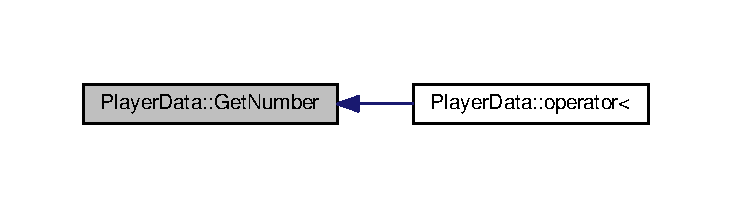
\includegraphics[width=350pt]{class_player_data_a0597b5d7c731ad08862eff9f5fb48754_icgraph}
\end{center}
\end{figure}


\hypertarget{class_player_data_af3ec6bf093ef6ba0d2bc1497907d8c6c}{\index{Player\-Data@{Player\-Data}!Get\-Old\-Guid@{Get\-Old\-Guid}}
\index{Get\-Old\-Guid@{Get\-Old\-Guid}!PlayerData@{Player\-Data}}
\subsubsection[{Get\-Old\-Guid}]{\setlength{\rightskip}{0pt plus 5cm}std\-::string Player\-Data\-::\-Get\-Old\-Guid (
\begin{DoxyParamCaption}
{}
\end{DoxyParamCaption}
) const}}\label{class_player_data_af3ec6bf093ef6ba0d2bc1497907d8c6c}

\begin{DoxyCode}
198 \{
199     boost::mutex::scoped\_lock lock(\hyperlink{class_player_data_a8e1276aab88bec3fa48e3c59f193827e}{m\_dataMutex});
200     \textcolor{keywordflow}{return} \hyperlink{class_player_data_aac3ac77674157db291a3f49076bcb4bc}{m\_oldGuid};
201 \}
\end{DoxyCode}
\hypertarget{class_player_data_a6ec702f92553198aabca8a235dc2b995}{\index{Player\-Data@{Player\-Data}!Get\-Rights@{Get\-Rights}}
\index{Get\-Rights@{Get\-Rights}!PlayerData@{Player\-Data}}
\subsubsection[{Get\-Rights}]{\setlength{\rightskip}{0pt plus 5cm}{\bf Player\-Rights} Player\-Data\-::\-Get\-Rights (
\begin{DoxyParamCaption}
{}
\end{DoxyParamCaption}
) const}}\label{class_player_data_a6ec702f92553198aabca8a235dc2b995}

\begin{DoxyCode}
135 \{
136     boost::mutex::scoped\_lock lock(\hyperlink{class_player_data_a8e1276aab88bec3fa48e3c59f193827e}{m\_dataMutex});
137     \textcolor{keywordflow}{return} \hyperlink{class_player_data_aa764ce6a7e503e938865f52463c48d63}{m\_rights};
138 \}
\end{DoxyCode}
\hypertarget{class_player_data_a54eab50fb80ec7f18ce1777c3632a73d}{\index{Player\-Data@{Player\-Data}!Get\-Start\-Cash@{Get\-Start\-Cash}}
\index{Get\-Start\-Cash@{Get\-Start\-Cash}!PlayerData@{Player\-Data}}
\subsubsection[{Get\-Start\-Cash}]{\setlength{\rightskip}{0pt plus 5cm}int Player\-Data\-::\-Get\-Start\-Cash (
\begin{DoxyParamCaption}
{}
\end{DoxyParamCaption}
) const}}\label{class_player_data_a54eab50fb80ec7f18ce1777c3632a73d}

\begin{DoxyCode}
226 \{
227     boost::mutex::scoped\_lock lock(\hyperlink{class_player_data_a8e1276aab88bec3fa48e3c59f193827e}{m\_dataMutex});
228     \textcolor{keywordflow}{return} \hyperlink{class_player_data_afb53d1b4126139cdc74b8322dab0094a}{m\_startCash};
229 \}
\end{DoxyCode}
\hypertarget{class_player_data_abfb06f847beee982e86ad29d03edc3b5}{\index{Player\-Data@{Player\-Data}!Get\-Type@{Get\-Type}}
\index{Get\-Type@{Get\-Type}!PlayerData@{Player\-Data}}
\subsubsection[{Get\-Type}]{\setlength{\rightskip}{0pt plus 5cm}{\bf Player\-Type} Player\-Data\-::\-Get\-Type (
\begin{DoxyParamCaption}
{}
\end{DoxyParamCaption}
) const}}\label{class_player_data_abfb06f847beee982e86ad29d03edc3b5}

\begin{DoxyCode}
121 \{
122     boost::mutex::scoped\_lock lock(\hyperlink{class_player_data_a8e1276aab88bec3fa48e3c59f193827e}{m\_dataMutex});
123     \textcolor{keywordflow}{return} \hyperlink{class_player_data_a3e4b8d9fcda3d2def5f0a79468a87903}{m\_type};
124 \}
\end{DoxyCode}
\hypertarget{class_player_data_a9922629a2ab29426703454a3b1554e38}{\index{Player\-Data@{Player\-Data}!Get\-Unique\-Id@{Get\-Unique\-Id}}
\index{Get\-Unique\-Id@{Get\-Unique\-Id}!PlayerData@{Player\-Data}}
\subsubsection[{Get\-Unique\-Id}]{\setlength{\rightskip}{0pt plus 5cm}unsigned Player\-Data\-::\-Get\-Unique\-Id (
\begin{DoxyParamCaption}
{}
\end{DoxyParamCaption}
) const}}\label{class_player_data_a9922629a2ab29426703454a3b1554e38}

\begin{DoxyCode}
163 \{
164     \textcolor{comment}{// const value - no mutex needed.}
165     \textcolor{keywordflow}{return} \hyperlink{class_player_data_a2b6ed5c114b242c39eab3ec7c6622a5f}{m\_uniqueId};
166 \}
\end{DoxyCode}
\hypertarget{class_player_data_a0203b2a5c2042d46f0ca838c94db88fc}{\index{Player\-Data@{Player\-Data}!Is\-Game\-Admin@{Is\-Game\-Admin}}
\index{Is\-Game\-Admin@{Is\-Game\-Admin}!PlayerData@{Player\-Data}}
\subsubsection[{Is\-Game\-Admin}]{\setlength{\rightskip}{0pt plus 5cm}bool Player\-Data\-::\-Is\-Game\-Admin (
\begin{DoxyParamCaption}
{}
\end{DoxyParamCaption}
) const}}\label{class_player_data_a0203b2a5c2042d46f0ca838c94db88fc}

\begin{DoxyCode}
149 \{
150     boost::mutex::scoped\_lock lock(\hyperlink{class_player_data_a8e1276aab88bec3fa48e3c59f193827e}{m\_dataMutex});
151     \textcolor{keywordflow}{return} \hyperlink{class_player_data_ad7c207bf8ecc38e2f86bdd8d83c935df}{m\_isGameAdmin};
152 \}
\end{DoxyCode}
\hypertarget{class_player_data_afa03422cfe10bf02083f65746e2fb723}{\index{Player\-Data@{Player\-Data}!operator$<$@{operator$<$}}
\index{operator$<$@{operator$<$}!PlayerData@{Player\-Data}}
\subsubsection[{operator$<$}]{\setlength{\rightskip}{0pt plus 5cm}bool Player\-Data\-::operator$<$ (
\begin{DoxyParamCaption}
\item[{const {\bf Player\-Data} \&}]{other}
\end{DoxyParamCaption}
) const}}\label{class_player_data_afa03422cfe10bf02083f65746e2fb723}

\begin{DoxyCode}
240 \{
241     boost::mutex::scoped\_lock lock(\hyperlink{class_player_data_a8e1276aab88bec3fa48e3c59f193827e}{m\_dataMutex});
242     \textcolor{keywordflow}{return} \hyperlink{class_player_data_a00807837606a10faee2849b979181402}{m\_number} < other.\hyperlink{class_player_data_a0597b5d7c731ad08862eff9f5fb48754}{GetNumber}();
243 \}\end{DoxyCode}


이 함수 내부에서 호출하는 함수들에 대한 그래프입니다.\-:\nopagebreak
\begin{figure}[H]
\begin{center}
\leavevmode
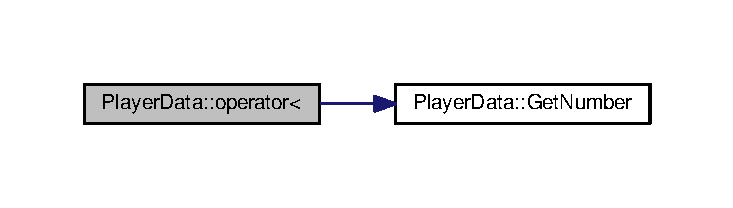
\includegraphics[width=350pt]{class_player_data_afa03422cfe10bf02083f65746e2fb723_cgraph}
\end{center}
\end{figure}


\hypertarget{class_player_data_a8174f11d0740db3f312c6b13fb2fe737}{\index{Player\-Data@{Player\-Data}!Set\-Avatar\-File@{Set\-Avatar\-File}}
\index{Set\-Avatar\-File@{Set\-Avatar\-File}!PlayerData@{Player\-Data}}
\subsubsection[{Set\-Avatar\-File}]{\setlength{\rightskip}{0pt plus 5cm}void Player\-Data\-::\-Set\-Avatar\-File (
\begin{DoxyParamCaption}
\item[{const std\-::string \&}]{avatar\-File}
\end{DoxyParamCaption}
)}}\label{class_player_data_a8174f11d0740db3f312c6b13fb2fe737}

\begin{DoxyCode}
89 \{
90     boost::mutex::scoped\_lock lock(\hyperlink{class_player_data_a8e1276aab88bec3fa48e3c59f193827e}{m\_dataMutex});
91     \hyperlink{class_player_data_aa3342ab34d521ab87edd40ec7622be56}{m\_avatarFile} = avatarFile;
92 \}
\end{DoxyCode}
\hypertarget{class_player_data_a57ed0efa276e6a62add8cf6ae0f1e54f}{\index{Player\-Data@{Player\-Data}!Set\-Avatar\-M\-D5@{Set\-Avatar\-M\-D5}}
\index{Set\-Avatar\-M\-D5@{Set\-Avatar\-M\-D5}!PlayerData@{Player\-Data}}
\subsubsection[{Set\-Avatar\-M\-D5}]{\setlength{\rightskip}{0pt plus 5cm}void Player\-Data\-::\-Set\-Avatar\-M\-D5 (
\begin{DoxyParamCaption}
\item[{const M\-D5\-Buf \&}]{avatar\-M\-D5}
\end{DoxyParamCaption}
)}}\label{class_player_data_a57ed0efa276e6a62add8cf6ae0f1e54f}

\begin{DoxyCode}
102 \{
103     boost::mutex::scoped\_lock lock(\hyperlink{class_player_data_a8e1276aab88bec3fa48e3c59f193827e}{m\_dataMutex});
104     \hyperlink{class_player_data_a5a6b19ae010990245ed6214be517f2cf}{m\_avatarMD5} = avatarMD5;
105 \}
\end{DoxyCode}
\hypertarget{class_player_data_aeb99c2c6ed25af7cfd46849bef370f4f}{\index{Player\-Data@{Player\-Data}!Set\-Country@{Set\-Country}}
\index{Set\-Country@{Set\-Country}!PlayerData@{Player\-Data}}
\subsubsection[{Set\-Country}]{\setlength{\rightskip}{0pt plus 5cm}void Player\-Data\-::\-Set\-Country (
\begin{DoxyParamCaption}
\item[{const std\-::string \&}]{country}
\end{DoxyParamCaption}
)}}\label{class_player_data_aeb99c2c6ed25af7cfd46849bef370f4f}

\begin{DoxyCode}
75 \{
76     boost::mutex::scoped\_lock lock(\hyperlink{class_player_data_a8e1276aab88bec3fa48e3c59f193827e}{m\_dataMutex});
77     \hyperlink{class_player_data_af349fdb550aaac72ccaead9a156be844}{m\_country} = country;
78 \}
\end{DoxyCode}
\hypertarget{class_player_data_a0f20856a42691cc4f917763307f895e0}{\index{Player\-Data@{Player\-Data}!Set\-D\-B\-Id@{Set\-D\-B\-Id}}
\index{Set\-D\-B\-Id@{Set\-D\-B\-Id}!PlayerData@{Player\-Data}}
\subsubsection[{Set\-D\-B\-Id}]{\setlength{\rightskip}{0pt plus 5cm}void Player\-Data\-::\-Set\-D\-B\-Id (
\begin{DoxyParamCaption}
\item[{D\-B\-\_\-id}]{id}
\end{DoxyParamCaption}
)}}\label{class_player_data_a0f20856a42691cc4f917763307f895e0}

\begin{DoxyCode}
219 \{
220     boost::mutex::scoped\_lock lock(\hyperlink{class_player_data_a8e1276aab88bec3fa48e3c59f193827e}{m\_dataMutex});
221     \hyperlink{class_player_data_af4a330231d9309b6e703f4c4fda251a8}{m\_dbId} = id;
222 \}
\end{DoxyCode}
\hypertarget{class_player_data_a926cfc7ff5a727ae5c0e072f0a1e947e}{\index{Player\-Data@{Player\-Data}!Set\-Game\-Admin@{Set\-Game\-Admin}}
\index{Set\-Game\-Admin@{Set\-Game\-Admin}!PlayerData@{Player\-Data}}
\subsubsection[{Set\-Game\-Admin}]{\setlength{\rightskip}{0pt plus 5cm}void Player\-Data\-::\-Set\-Game\-Admin (
\begin{DoxyParamCaption}
\item[{bool}]{is\-Admin}
\end{DoxyParamCaption}
)}}\label{class_player_data_a926cfc7ff5a727ae5c0e072f0a1e947e}

\begin{DoxyCode}
156 \{
157     boost::mutex::scoped\_lock lock(\hyperlink{class_player_data_a8e1276aab88bec3fa48e3c59f193827e}{m\_dataMutex});
158     \hyperlink{class_player_data_ad7c207bf8ecc38e2f86bdd8d83c935df}{m\_isGameAdmin} = isAdmin;
159 \}
\end{DoxyCode}
\hypertarget{class_player_data_ae6df82d891bb33d3d6ebe7e42d9bff07}{\index{Player\-Data@{Player\-Data}!Set\-Guid@{Set\-Guid}}
\index{Set\-Guid@{Set\-Guid}!PlayerData@{Player\-Data}}
\subsubsection[{Set\-Guid}]{\setlength{\rightskip}{0pt plus 5cm}void Player\-Data\-::\-Set\-Guid (
\begin{DoxyParamCaption}
\item[{const std\-::string \&}]{guid}
\end{DoxyParamCaption}
)}}\label{class_player_data_ae6df82d891bb33d3d6ebe7e42d9bff07}

\begin{DoxyCode}
191 \{
192     boost::mutex::scoped\_lock lock(\hyperlink{class_player_data_a8e1276aab88bec3fa48e3c59f193827e}{m\_dataMutex});
193     \hyperlink{class_player_data_a3d3abd9ce7a8421596ce2ec2bf16bd64}{m\_guid} = guid;
194 \}
\end{DoxyCode}
\hypertarget{class_player_data_a0ce3965e0a0baf505eca8e13d7580f19}{\index{Player\-Data@{Player\-Data}!Set\-Name@{Set\-Name}}
\index{Set\-Name@{Set\-Name}!PlayerData@{Player\-Data}}
\subsubsection[{Set\-Name}]{\setlength{\rightskip}{0pt plus 5cm}void Player\-Data\-::\-Set\-Name (
\begin{DoxyParamCaption}
\item[{const std\-::string \&}]{name}
\end{DoxyParamCaption}
)}}\label{class_player_data_a0ce3965e0a0baf505eca8e13d7580f19}

\begin{DoxyCode}
61 \{
62     boost::mutex::scoped\_lock lock(\hyperlink{class_player_data_a8e1276aab88bec3fa48e3c59f193827e}{m\_dataMutex});
63     \hyperlink{class_player_data_a0174f971f59af5008301ac6eb3d2304c}{m\_name} = name;
64 \}
\end{DoxyCode}
\hypertarget{class_player_data_ac3d0ad92de2c8e42f7df88b40e75003d}{\index{Player\-Data@{Player\-Data}!Set\-Net\-Avatar\-File@{Set\-Net\-Avatar\-File}}
\index{Set\-Net\-Avatar\-File@{Set\-Net\-Avatar\-File}!PlayerData@{Player\-Data}}
\subsubsection[{Set\-Net\-Avatar\-File}]{\setlength{\rightskip}{0pt plus 5cm}void Player\-Data\-::\-Set\-Net\-Avatar\-File (
\begin{DoxyParamCaption}
\item[{boost\-::shared\-\_\-ptr$<$ {\bf Avatar\-File} $>$}]{Avatar\-File}
\end{DoxyParamCaption}
)}}\label{class_player_data_ac3d0ad92de2c8e42f7df88b40e75003d}

\begin{DoxyCode}
115 \{
116     \hyperlink{class_player_data_afafb202de188ebee15e54b49aa96feac}{m\_netAvatarFile} = \hyperlink{struct_avatar_file}{AvatarFile};
117 \}
\end{DoxyCode}
\hypertarget{class_player_data_acc626969fae365d9a85134c1602620de}{\index{Player\-Data@{Player\-Data}!Set\-Number@{Set\-Number}}
\index{Set\-Number@{Set\-Number}!PlayerData@{Player\-Data}}
\subsubsection[{Set\-Number}]{\setlength{\rightskip}{0pt plus 5cm}void Player\-Data\-::\-Set\-Number (
\begin{DoxyParamCaption}
\item[{int}]{number}
\end{DoxyParamCaption}
)}}\label{class_player_data_acc626969fae365d9a85134c1602620de}

\begin{DoxyCode}
177 \{
178     boost::mutex::scoped\_lock lock(\hyperlink{class_player_data_a8e1276aab88bec3fa48e3c59f193827e}{m\_dataMutex});
179     \hyperlink{class_player_data_a00807837606a10faee2849b979181402}{m\_number} = number;
180 \}
\end{DoxyCode}
\hypertarget{class_player_data_a575e319875bdd901034d54be2f88ea12}{\index{Player\-Data@{Player\-Data}!Set\-Old\-Guid@{Set\-Old\-Guid}}
\index{Set\-Old\-Guid@{Set\-Old\-Guid}!PlayerData@{Player\-Data}}
\subsubsection[{Set\-Old\-Guid}]{\setlength{\rightskip}{0pt plus 5cm}void Player\-Data\-::\-Set\-Old\-Guid (
\begin{DoxyParamCaption}
\item[{const std\-::string \&}]{guid}
\end{DoxyParamCaption}
)}}\label{class_player_data_a575e319875bdd901034d54be2f88ea12}

\begin{DoxyCode}
205 \{
206     boost::mutex::scoped\_lock lock(\hyperlink{class_player_data_a8e1276aab88bec3fa48e3c59f193827e}{m\_dataMutex});
207     \hyperlink{class_player_data_aac3ac77674157db291a3f49076bcb4bc}{m\_oldGuid} = guid;
208 \}
\end{DoxyCode}
\hypertarget{class_player_data_a6496cec308484ed8f3ef100721d6461d}{\index{Player\-Data@{Player\-Data}!Set\-Rights@{Set\-Rights}}
\index{Set\-Rights@{Set\-Rights}!PlayerData@{Player\-Data}}
\subsubsection[{Set\-Rights}]{\setlength{\rightskip}{0pt plus 5cm}void Player\-Data\-::\-Set\-Rights (
\begin{DoxyParamCaption}
\item[{{\bf Player\-Rights}}]{rights}
\end{DoxyParamCaption}
)}}\label{class_player_data_a6496cec308484ed8f3ef100721d6461d}

\begin{DoxyCode}
142 \{
143     boost::mutex::scoped\_lock lock(\hyperlink{class_player_data_a8e1276aab88bec3fa48e3c59f193827e}{m\_dataMutex});
144     \hyperlink{class_player_data_aa764ce6a7e503e938865f52463c48d63}{m\_rights} = rights;
145 \}
\end{DoxyCode}
\hypertarget{class_player_data_ab0b58b77fb2366c31ff902cd91117919}{\index{Player\-Data@{Player\-Data}!Set\-Start\-Cash@{Set\-Start\-Cash}}
\index{Set\-Start\-Cash@{Set\-Start\-Cash}!PlayerData@{Player\-Data}}
\subsubsection[{Set\-Start\-Cash}]{\setlength{\rightskip}{0pt plus 5cm}void Player\-Data\-::\-Set\-Start\-Cash (
\begin{DoxyParamCaption}
\item[{int}]{cash}
\end{DoxyParamCaption}
)}}\label{class_player_data_ab0b58b77fb2366c31ff902cd91117919}

\begin{DoxyCode}
233 \{
234     boost::mutex::scoped\_lock lock(\hyperlink{class_player_data_a8e1276aab88bec3fa48e3c59f193827e}{m\_dataMutex});
235     \hyperlink{class_player_data_afb53d1b4126139cdc74b8322dab0094a}{m\_startCash} = cash;
236 \}
\end{DoxyCode}
\hypertarget{class_player_data_a8a32bc6cc032cccbab4d761054f8578a}{\index{Player\-Data@{Player\-Data}!Set\-Type@{Set\-Type}}
\index{Set\-Type@{Set\-Type}!PlayerData@{Player\-Data}}
\subsubsection[{Set\-Type}]{\setlength{\rightskip}{0pt plus 5cm}void Player\-Data\-::\-Set\-Type (
\begin{DoxyParamCaption}
\item[{{\bf Player\-Type}}]{type}
\end{DoxyParamCaption}
)}}\label{class_player_data_a8a32bc6cc032cccbab4d761054f8578a}

\begin{DoxyCode}
128 \{
129     boost::mutex::scoped\_lock lock(\hyperlink{class_player_data_a8e1276aab88bec3fa48e3c59f193827e}{m\_dataMutex});
130     \hyperlink{class_player_data_a3e4b8d9fcda3d2def5f0a79468a87903}{m\_type} = type;
131 \}
\end{DoxyCode}


\subsection{멤버 데이타 문서화}
\hypertarget{class_player_data_aa3342ab34d521ab87edd40ec7622be56}{\index{Player\-Data@{Player\-Data}!m\-\_\-avatar\-File@{m\-\_\-avatar\-File}}
\index{m\-\_\-avatar\-File@{m\-\_\-avatar\-File}!PlayerData@{Player\-Data}}
\subsubsection[{m\-\_\-avatar\-File}]{\setlength{\rightskip}{0pt plus 5cm}std\-::string Player\-Data\-::m\-\_\-avatar\-File\hspace{0.3cm}{\ttfamily [private]}}}\label{class_player_data_aa3342ab34d521ab87edd40ec7622be56}
\hypertarget{class_player_data_a5a6b19ae010990245ed6214be517f2cf}{\index{Player\-Data@{Player\-Data}!m\-\_\-avatar\-M\-D5@{m\-\_\-avatar\-M\-D5}}
\index{m\-\_\-avatar\-M\-D5@{m\-\_\-avatar\-M\-D5}!PlayerData@{Player\-Data}}
\subsubsection[{m\-\_\-avatar\-M\-D5}]{\setlength{\rightskip}{0pt plus 5cm}M\-D5\-Buf Player\-Data\-::m\-\_\-avatar\-M\-D5\hspace{0.3cm}{\ttfamily [private]}}}\label{class_player_data_a5a6b19ae010990245ed6214be517f2cf}
\hypertarget{class_player_data_af349fdb550aaac72ccaead9a156be844}{\index{Player\-Data@{Player\-Data}!m\-\_\-country@{m\-\_\-country}}
\index{m\-\_\-country@{m\-\_\-country}!PlayerData@{Player\-Data}}
\subsubsection[{m\-\_\-country}]{\setlength{\rightskip}{0pt plus 5cm}std\-::string Player\-Data\-::m\-\_\-country\hspace{0.3cm}{\ttfamily [private]}}}\label{class_player_data_af349fdb550aaac72ccaead9a156be844}
\hypertarget{class_player_data_a8e1276aab88bec3fa48e3c59f193827e}{\index{Player\-Data@{Player\-Data}!m\-\_\-data\-Mutex@{m\-\_\-data\-Mutex}}
\index{m\-\_\-data\-Mutex@{m\-\_\-data\-Mutex}!PlayerData@{Player\-Data}}
\subsubsection[{m\-\_\-data\-Mutex}]{\setlength{\rightskip}{0pt plus 5cm}boost\-::mutex Player\-Data\-::m\-\_\-data\-Mutex\hspace{0.3cm}{\ttfamily [mutable]}, {\ttfamily [private]}}}\label{class_player_data_a8e1276aab88bec3fa48e3c59f193827e}
\hypertarget{class_player_data_af4a330231d9309b6e703f4c4fda251a8}{\index{Player\-Data@{Player\-Data}!m\-\_\-db\-Id@{m\-\_\-db\-Id}}
\index{m\-\_\-db\-Id@{m\-\_\-db\-Id}!PlayerData@{Player\-Data}}
\subsubsection[{m\-\_\-db\-Id}]{\setlength{\rightskip}{0pt plus 5cm}D\-B\-\_\-id Player\-Data\-::m\-\_\-db\-Id\hspace{0.3cm}{\ttfamily [private]}}}\label{class_player_data_af4a330231d9309b6e703f4c4fda251a8}
\hypertarget{class_player_data_a3d3abd9ce7a8421596ce2ec2bf16bd64}{\index{Player\-Data@{Player\-Data}!m\-\_\-guid@{m\-\_\-guid}}
\index{m\-\_\-guid@{m\-\_\-guid}!PlayerData@{Player\-Data}}
\subsubsection[{m\-\_\-guid}]{\setlength{\rightskip}{0pt plus 5cm}std\-::string Player\-Data\-::m\-\_\-guid\hspace{0.3cm}{\ttfamily [private]}}}\label{class_player_data_a3d3abd9ce7a8421596ce2ec2bf16bd64}
\hypertarget{class_player_data_ad7c207bf8ecc38e2f86bdd8d83c935df}{\index{Player\-Data@{Player\-Data}!m\-\_\-is\-Game\-Admin@{m\-\_\-is\-Game\-Admin}}
\index{m\-\_\-is\-Game\-Admin@{m\-\_\-is\-Game\-Admin}!PlayerData@{Player\-Data}}
\subsubsection[{m\-\_\-is\-Game\-Admin}]{\setlength{\rightskip}{0pt plus 5cm}bool Player\-Data\-::m\-\_\-is\-Game\-Admin\hspace{0.3cm}{\ttfamily [private]}}}\label{class_player_data_ad7c207bf8ecc38e2f86bdd8d83c935df}
\hypertarget{class_player_data_a0174f971f59af5008301ac6eb3d2304c}{\index{Player\-Data@{Player\-Data}!m\-\_\-name@{m\-\_\-name}}
\index{m\-\_\-name@{m\-\_\-name}!PlayerData@{Player\-Data}}
\subsubsection[{m\-\_\-name}]{\setlength{\rightskip}{0pt plus 5cm}std\-::string Player\-Data\-::m\-\_\-name\hspace{0.3cm}{\ttfamily [private]}}}\label{class_player_data_a0174f971f59af5008301ac6eb3d2304c}
\hypertarget{class_player_data_afafb202de188ebee15e54b49aa96feac}{\index{Player\-Data@{Player\-Data}!m\-\_\-net\-Avatar\-File@{m\-\_\-net\-Avatar\-File}}
\index{m\-\_\-net\-Avatar\-File@{m\-\_\-net\-Avatar\-File}!PlayerData@{Player\-Data}}
\subsubsection[{m\-\_\-net\-Avatar\-File}]{\setlength{\rightskip}{0pt plus 5cm}boost\-::shared\-\_\-ptr$<${\bf Avatar\-File}$>$ Player\-Data\-::m\-\_\-net\-Avatar\-File\hspace{0.3cm}{\ttfamily [private]}}}\label{class_player_data_afafb202de188ebee15e54b49aa96feac}
\hypertarget{class_player_data_a00807837606a10faee2849b979181402}{\index{Player\-Data@{Player\-Data}!m\-\_\-number@{m\-\_\-number}}
\index{m\-\_\-number@{m\-\_\-number}!PlayerData@{Player\-Data}}
\subsubsection[{m\-\_\-number}]{\setlength{\rightskip}{0pt plus 5cm}int Player\-Data\-::m\-\_\-number\hspace{0.3cm}{\ttfamily [private]}}}\label{class_player_data_a00807837606a10faee2849b979181402}
\hypertarget{class_player_data_aac3ac77674157db291a3f49076bcb4bc}{\index{Player\-Data@{Player\-Data}!m\-\_\-old\-Guid@{m\-\_\-old\-Guid}}
\index{m\-\_\-old\-Guid@{m\-\_\-old\-Guid}!PlayerData@{Player\-Data}}
\subsubsection[{m\-\_\-old\-Guid}]{\setlength{\rightskip}{0pt plus 5cm}std\-::string Player\-Data\-::m\-\_\-old\-Guid\hspace{0.3cm}{\ttfamily [private]}}}\label{class_player_data_aac3ac77674157db291a3f49076bcb4bc}
\hypertarget{class_player_data_a2cbffcef76225936b3860adcd0ab6e03}{\index{Player\-Data@{Player\-Data}!m\-\_\-password@{m\-\_\-password}}
\index{m\-\_\-password@{m\-\_\-password}!PlayerData@{Player\-Data}}
\subsubsection[{m\-\_\-password}]{\setlength{\rightskip}{0pt plus 5cm}std\-::string Player\-Data\-::m\-\_\-password\hspace{0.3cm}{\ttfamily [private]}}}\label{class_player_data_a2cbffcef76225936b3860adcd0ab6e03}
\hypertarget{class_player_data_aa764ce6a7e503e938865f52463c48d63}{\index{Player\-Data@{Player\-Data}!m\-\_\-rights@{m\-\_\-rights}}
\index{m\-\_\-rights@{m\-\_\-rights}!PlayerData@{Player\-Data}}
\subsubsection[{m\-\_\-rights}]{\setlength{\rightskip}{0pt plus 5cm}{\bf Player\-Rights} Player\-Data\-::m\-\_\-rights\hspace{0.3cm}{\ttfamily [private]}}}\label{class_player_data_aa764ce6a7e503e938865f52463c48d63}
\hypertarget{class_player_data_afb53d1b4126139cdc74b8322dab0094a}{\index{Player\-Data@{Player\-Data}!m\-\_\-start\-Cash@{m\-\_\-start\-Cash}}
\index{m\-\_\-start\-Cash@{m\-\_\-start\-Cash}!PlayerData@{Player\-Data}}
\subsubsection[{m\-\_\-start\-Cash}]{\setlength{\rightskip}{0pt plus 5cm}int Player\-Data\-::m\-\_\-start\-Cash\hspace{0.3cm}{\ttfamily [private]}}}\label{class_player_data_afb53d1b4126139cdc74b8322dab0094a}
\hypertarget{class_player_data_a3e4b8d9fcda3d2def5f0a79468a87903}{\index{Player\-Data@{Player\-Data}!m\-\_\-type@{m\-\_\-type}}
\index{m\-\_\-type@{m\-\_\-type}!PlayerData@{Player\-Data}}
\subsubsection[{m\-\_\-type}]{\setlength{\rightskip}{0pt plus 5cm}{\bf Player\-Type} Player\-Data\-::m\-\_\-type\hspace{0.3cm}{\ttfamily [private]}}}\label{class_player_data_a3e4b8d9fcda3d2def5f0a79468a87903}
\hypertarget{class_player_data_a2b6ed5c114b242c39eab3ec7c6622a5f}{\index{Player\-Data@{Player\-Data}!m\-\_\-unique\-Id@{m\-\_\-unique\-Id}}
\index{m\-\_\-unique\-Id@{m\-\_\-unique\-Id}!PlayerData@{Player\-Data}}
\subsubsection[{m\-\_\-unique\-Id}]{\setlength{\rightskip}{0pt plus 5cm}const unsigned Player\-Data\-::m\-\_\-unique\-Id\hspace{0.3cm}{\ttfamily [private]}}}\label{class_player_data_a2b6ed5c114b242c39eab3ec7c6622a5f}


이 클래스에 대한 문서화 페이지는 다음의 파일들로부터 생성되었습니다.\-:\begin{DoxyCompactItemize}
\item 
\hyperlink{playerdata_8h}{playerdata.\-h}\item 
\hyperlink{playerdata_8cpp}{playerdata.\-cpp}\end{DoxyCompactItemize}

\hypertarget{struct_player_info}{\section{Player\-Info 구조체 참조}
\label{struct_player_info}\index{Player\-Info@{Player\-Info}}
}


{\ttfamily \#include $<$playerdata.\-h$>$}



Player\-Info에 대한 협력 다이어그램\-:\nopagebreak
\begin{figure}[H]
\begin{center}
\leavevmode
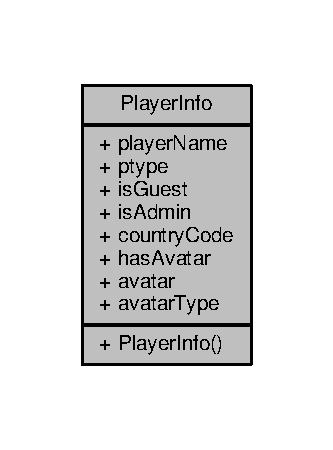
\includegraphics[width=160pt]{struct_player_info__coll__graph}
\end{center}
\end{figure}
\subsection*{Public 멤버 함수}
\begin{DoxyCompactItemize}
\item 
\hyperlink{struct_player_info_a05e9b9529ed8e4638b2bd2fb76b3abeb}{Player\-Info} ()
\end{DoxyCompactItemize}
\subsection*{Public 속성}
\begin{DoxyCompactItemize}
\item 
std\-::string \hyperlink{struct_player_info_a3d3262624b58928b67d59b6049995510}{player\-Name}
\item 
\hyperlink{playerdata_8h_abe590f3c9109f404f003d5d7e4f0fccf}{Player\-Type} \hyperlink{struct_player_info_ad5f6464116a3777bd7e3316ac58862d0}{ptype}
\item 
bool \hyperlink{struct_player_info_a486ef88d7337edab71e381c212f062f2}{is\-Guest}
\item 
bool \hyperlink{struct_player_info_a0455fa7d311c4e3cc9cb29f491fdc640}{is\-Admin}
\item 
std\-::string \hyperlink{struct_player_info_acecb2609d2339d02b3a9976f3128b1cb}{country\-Code}
\item 
bool \hyperlink{struct_player_info_aa6c0789c0583911d456c80ee3f0b9eef}{has\-Avatar}
\item 
M\-D5\-Buf \hyperlink{struct_player_info_a7c57fe28d4955552bbdcd27a50d98574}{avatar}
\item 
\hyperlink{playerdata_8h_a838468e0dd027767b891761d30d2bf39}{Avatar\-File\-Type} \hyperlink{struct_player_info_a57c48e192309aeabb51d758898b588d9}{avatar\-Type}
\end{DoxyCompactItemize}


\subsection{생성자 \& 소멸자 문서화}
\hypertarget{struct_player_info_a05e9b9529ed8e4638b2bd2fb76b3abeb}{\index{Player\-Info@{Player\-Info}!Player\-Info@{Player\-Info}}
\index{Player\-Info@{Player\-Info}!PlayerInfo@{Player\-Info}}
\subsubsection[{Player\-Info}]{\setlength{\rightskip}{0pt plus 5cm}Player\-Info\-::\-Player\-Info (
\begin{DoxyParamCaption}
{}
\end{DoxyParamCaption}
)\hspace{0.3cm}{\ttfamily [inline]}}}\label{struct_player_info_a05e9b9529ed8e4638b2bd2fb76b3abeb}

\begin{DoxyCode}
73 : \hyperlink{struct_player_info_ad5f6464116a3777bd7e3316ac58862d0}{ptype}(\hyperlink{playerdata_8h_abe590f3c9109f404f003d5d7e4f0fccfa6bf6033830c666c7491c430f7ff395a0}{PLAYER\_TYPE\_HUMAN}), \hyperlink{struct_player_info_a486ef88d7337edab71e381c212f062f2}{isGuest}(\textcolor{keyword}{false}), \hyperlink{struct_player_info_a0455fa7d311c4e3cc9cb29f491fdc640}{isAdmin}(\textcolor{keyword}{false}), 
      \hyperlink{struct_player_info_aa6c0789c0583911d456c80ee3f0b9eef}{hasAvatar}(\textcolor{keyword}{false}), \hyperlink{struct_player_info_a57c48e192309aeabb51d758898b588d9}{avatarType}(\hyperlink{playerdata_8h_a838468e0dd027767b891761d30d2bf39af3195e1aaeb82da02f85ea7a293e91a1}{AVATAR\_FILE\_TYPE\_UNKNOWN}) \{\}
\end{DoxyCode}


\subsection{멤버 데이타 문서화}
\hypertarget{struct_player_info_a7c57fe28d4955552bbdcd27a50d98574}{\index{Player\-Info@{Player\-Info}!avatar@{avatar}}
\index{avatar@{avatar}!PlayerInfo@{Player\-Info}}
\subsubsection[{avatar}]{\setlength{\rightskip}{0pt plus 5cm}M\-D5\-Buf Player\-Info\-::avatar}}\label{struct_player_info_a7c57fe28d4955552bbdcd27a50d98574}
\hypertarget{struct_player_info_a57c48e192309aeabb51d758898b588d9}{\index{Player\-Info@{Player\-Info}!avatar\-Type@{avatar\-Type}}
\index{avatar\-Type@{avatar\-Type}!PlayerInfo@{Player\-Info}}
\subsubsection[{avatar\-Type}]{\setlength{\rightskip}{0pt plus 5cm}{\bf Avatar\-File\-Type} Player\-Info\-::avatar\-Type}}\label{struct_player_info_a57c48e192309aeabb51d758898b588d9}
\hypertarget{struct_player_info_acecb2609d2339d02b3a9976f3128b1cb}{\index{Player\-Info@{Player\-Info}!country\-Code@{country\-Code}}
\index{country\-Code@{country\-Code}!PlayerInfo@{Player\-Info}}
\subsubsection[{country\-Code}]{\setlength{\rightskip}{0pt plus 5cm}std\-::string Player\-Info\-::country\-Code}}\label{struct_player_info_acecb2609d2339d02b3a9976f3128b1cb}
\hypertarget{struct_player_info_aa6c0789c0583911d456c80ee3f0b9eef}{\index{Player\-Info@{Player\-Info}!has\-Avatar@{has\-Avatar}}
\index{has\-Avatar@{has\-Avatar}!PlayerInfo@{Player\-Info}}
\subsubsection[{has\-Avatar}]{\setlength{\rightskip}{0pt plus 5cm}bool Player\-Info\-::has\-Avatar}}\label{struct_player_info_aa6c0789c0583911d456c80ee3f0b9eef}
\hypertarget{struct_player_info_a0455fa7d311c4e3cc9cb29f491fdc640}{\index{Player\-Info@{Player\-Info}!is\-Admin@{is\-Admin}}
\index{is\-Admin@{is\-Admin}!PlayerInfo@{Player\-Info}}
\subsubsection[{is\-Admin}]{\setlength{\rightskip}{0pt plus 5cm}bool Player\-Info\-::is\-Admin}}\label{struct_player_info_a0455fa7d311c4e3cc9cb29f491fdc640}
\hypertarget{struct_player_info_a486ef88d7337edab71e381c212f062f2}{\index{Player\-Info@{Player\-Info}!is\-Guest@{is\-Guest}}
\index{is\-Guest@{is\-Guest}!PlayerInfo@{Player\-Info}}
\subsubsection[{is\-Guest}]{\setlength{\rightskip}{0pt plus 5cm}bool Player\-Info\-::is\-Guest}}\label{struct_player_info_a486ef88d7337edab71e381c212f062f2}
\hypertarget{struct_player_info_a3d3262624b58928b67d59b6049995510}{\index{Player\-Info@{Player\-Info}!player\-Name@{player\-Name}}
\index{player\-Name@{player\-Name}!PlayerInfo@{Player\-Info}}
\subsubsection[{player\-Name}]{\setlength{\rightskip}{0pt plus 5cm}std\-::string Player\-Info\-::player\-Name}}\label{struct_player_info_a3d3262624b58928b67d59b6049995510}
\hypertarget{struct_player_info_ad5f6464116a3777bd7e3316ac58862d0}{\index{Player\-Info@{Player\-Info}!ptype@{ptype}}
\index{ptype@{ptype}!PlayerInfo@{Player\-Info}}
\subsubsection[{ptype}]{\setlength{\rightskip}{0pt plus 5cm}{\bf Player\-Type} Player\-Info\-::ptype}}\label{struct_player_info_ad5f6464116a3777bd7e3316ac58862d0}


이 구조체에 대한 문서화 페이지는 다음의 파일로부터 생성되었습니다.\-:\begin{DoxyCompactItemize}
\item 
\hyperlink{playerdata_8h}{playerdata.\-h}\end{DoxyCompactItemize}

\hypertarget{struct_server_info}{\section{Server\-Info 구조체 참조}
\label{struct_server_info}\index{Server\-Info@{Server\-Info}}
}


{\ttfamily \#include $<$serverdata.\-h$>$}



Server\-Info에 대한 협력 다이어그램\-:\nopagebreak
\begin{figure}[H]
\begin{center}
\leavevmode
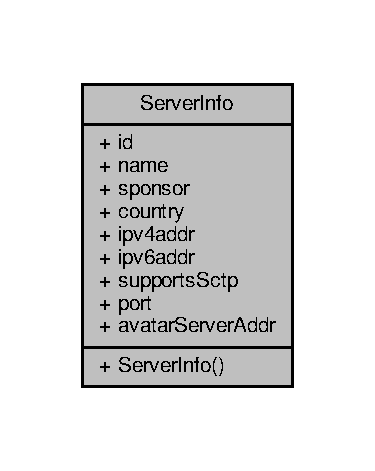
\includegraphics[width=180pt]{struct_server_info__coll__graph}
\end{center}
\end{figure}
\subsection*{Public 멤버 함수}
\begin{DoxyCompactItemize}
\item 
\hyperlink{struct_server_info_a7627924fa461528a5c0a13b105499410}{Server\-Info} ()
\end{DoxyCompactItemize}
\subsection*{Public 속성}
\begin{DoxyCompactItemize}
\item 
unsigned \hyperlink{struct_server_info_a016372aebe04fe8ddf9d17b8977c0805}{id}
\item 
std\-::string \hyperlink{struct_server_info_ac1b6c30ed482012324aee9a240007158}{name}
\item 
std\-::string \hyperlink{struct_server_info_a019cc206a894a80b8254bf3798173a25}{sponsor}
\item 
std\-::string \hyperlink{struct_server_info_a7c58f400c3f76c6c61d7455276943125}{country}
\item 
std\-::string \hyperlink{struct_server_info_af0fafe5df3594c377aa38b4f32adcd0f}{ipv4addr}
\item 
std\-::string \hyperlink{struct_server_info_ae37d24d79649b567857dd9765b7dba6d}{ipv6addr}
\item 
bool \hyperlink{struct_server_info_ad566c6729bf2eae019af64a50eb64f6b}{supports\-Sctp}
\item 
int \hyperlink{struct_server_info_a8af087c39c4cfaf845feba73ad1bd9af}{port}
\item 
std\-::string \hyperlink{struct_server_info_ab880c1acf33d44c50edb68df6226782d}{avatar\-Server\-Addr}
\end{DoxyCompactItemize}


\subsection{생성자 \& 소멸자 문서화}
\hypertarget{struct_server_info_a7627924fa461528a5c0a13b105499410}{\index{Server\-Info@{Server\-Info}!Server\-Info@{Server\-Info}}
\index{Server\-Info@{Server\-Info}!ServerInfo@{Server\-Info}}
\subsubsection[{Server\-Info}]{\setlength{\rightskip}{0pt plus 5cm}Server\-Info\-::\-Server\-Info (
\begin{DoxyParamCaption}
{}
\end{DoxyParamCaption}
)\hspace{0.3cm}{\ttfamily [inline]}}}\label{struct_server_info_a7627924fa461528a5c0a13b105499410}

\begin{DoxyCode}
39 : \hyperlink{struct_server_info_a016372aebe04fe8ddf9d17b8977c0805}{id}(0), \hyperlink{struct_server_info_ad566c6729bf2eae019af64a50eb64f6b}{supportsSctp}(\textcolor{keyword}{false}), \hyperlink{struct_server_info_a8af087c39c4cfaf845feba73ad1bd9af}{port}(0) \{\}
\end{DoxyCode}


\subsection{멤버 데이타 문서화}
\hypertarget{struct_server_info_ab880c1acf33d44c50edb68df6226782d}{\index{Server\-Info@{Server\-Info}!avatar\-Server\-Addr@{avatar\-Server\-Addr}}
\index{avatar\-Server\-Addr@{avatar\-Server\-Addr}!ServerInfo@{Server\-Info}}
\subsubsection[{avatar\-Server\-Addr}]{\setlength{\rightskip}{0pt plus 5cm}std\-::string Server\-Info\-::avatar\-Server\-Addr}}\label{struct_server_info_ab880c1acf33d44c50edb68df6226782d}
\hypertarget{struct_server_info_a7c58f400c3f76c6c61d7455276943125}{\index{Server\-Info@{Server\-Info}!country@{country}}
\index{country@{country}!ServerInfo@{Server\-Info}}
\subsubsection[{country}]{\setlength{\rightskip}{0pt plus 5cm}std\-::string Server\-Info\-::country}}\label{struct_server_info_a7c58f400c3f76c6c61d7455276943125}
\hypertarget{struct_server_info_a016372aebe04fe8ddf9d17b8977c0805}{\index{Server\-Info@{Server\-Info}!id@{id}}
\index{id@{id}!ServerInfo@{Server\-Info}}
\subsubsection[{id}]{\setlength{\rightskip}{0pt plus 5cm}unsigned Server\-Info\-::id}}\label{struct_server_info_a016372aebe04fe8ddf9d17b8977c0805}
\hypertarget{struct_server_info_af0fafe5df3594c377aa38b4f32adcd0f}{\index{Server\-Info@{Server\-Info}!ipv4addr@{ipv4addr}}
\index{ipv4addr@{ipv4addr}!ServerInfo@{Server\-Info}}
\subsubsection[{ipv4addr}]{\setlength{\rightskip}{0pt plus 5cm}std\-::string Server\-Info\-::ipv4addr}}\label{struct_server_info_af0fafe5df3594c377aa38b4f32adcd0f}
\hypertarget{struct_server_info_ae37d24d79649b567857dd9765b7dba6d}{\index{Server\-Info@{Server\-Info}!ipv6addr@{ipv6addr}}
\index{ipv6addr@{ipv6addr}!ServerInfo@{Server\-Info}}
\subsubsection[{ipv6addr}]{\setlength{\rightskip}{0pt plus 5cm}std\-::string Server\-Info\-::ipv6addr}}\label{struct_server_info_ae37d24d79649b567857dd9765b7dba6d}
\hypertarget{struct_server_info_ac1b6c30ed482012324aee9a240007158}{\index{Server\-Info@{Server\-Info}!name@{name}}
\index{name@{name}!ServerInfo@{Server\-Info}}
\subsubsection[{name}]{\setlength{\rightskip}{0pt plus 5cm}std\-::string Server\-Info\-::name}}\label{struct_server_info_ac1b6c30ed482012324aee9a240007158}
\hypertarget{struct_server_info_a8af087c39c4cfaf845feba73ad1bd9af}{\index{Server\-Info@{Server\-Info}!port@{port}}
\index{port@{port}!ServerInfo@{Server\-Info}}
\subsubsection[{port}]{\setlength{\rightskip}{0pt plus 5cm}int Server\-Info\-::port}}\label{struct_server_info_a8af087c39c4cfaf845feba73ad1bd9af}
\hypertarget{struct_server_info_a019cc206a894a80b8254bf3798173a25}{\index{Server\-Info@{Server\-Info}!sponsor@{sponsor}}
\index{sponsor@{sponsor}!ServerInfo@{Server\-Info}}
\subsubsection[{sponsor}]{\setlength{\rightskip}{0pt plus 5cm}std\-::string Server\-Info\-::sponsor}}\label{struct_server_info_a019cc206a894a80b8254bf3798173a25}
\hypertarget{struct_server_info_ad566c6729bf2eae019af64a50eb64f6b}{\index{Server\-Info@{Server\-Info}!supports\-Sctp@{supports\-Sctp}}
\index{supports\-Sctp@{supports\-Sctp}!ServerInfo@{Server\-Info}}
\subsubsection[{supports\-Sctp}]{\setlength{\rightskip}{0pt plus 5cm}bool Server\-Info\-::supports\-Sctp}}\label{struct_server_info_ad566c6729bf2eae019af64a50eb64f6b}


이 구조체에 대한 문서화 페이지는 다음의 파일로부터 생성되었습니다.\-:\begin{DoxyCompactItemize}
\item 
\hyperlink{serverdata_8h}{serverdata.\-h}\end{DoxyCompactItemize}

\hypertarget{struct_server_stats}{\section{Server\-Stats 구조체 참조}
\label{struct_server_stats}\index{Server\-Stats@{Server\-Stats}}
}


{\ttfamily \#include $<$serverdata.\-h$>$}



Server\-Stats에 대한 협력 다이어그램\-:\nopagebreak
\begin{figure}[H]
\begin{center}
\leavevmode
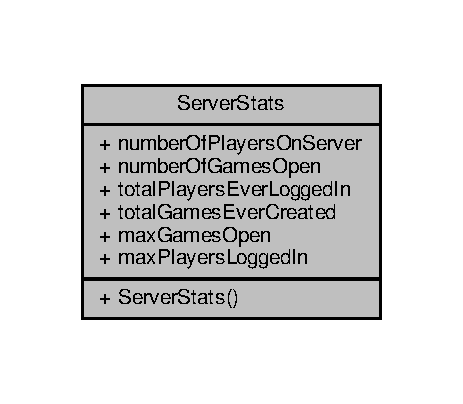
\includegraphics[width=222pt]{struct_server_stats__coll__graph}
\end{center}
\end{figure}
\subsection*{Public 멤버 함수}
\begin{DoxyCompactItemize}
\item 
\hyperlink{struct_server_stats_a1ed311eaeb034e47dd26f531114b9ad1}{Server\-Stats} ()
\end{DoxyCompactItemize}
\subsection*{Public 속성}
\begin{DoxyCompactItemize}
\item 
unsigned \hyperlink{struct_server_stats_ae5c627e4a9c50bf2ff6c037ec0bc81d0}{number\-Of\-Players\-On\-Server}
\item 
unsigned \hyperlink{struct_server_stats_a6718463c122b2cf94a315fd796084838}{number\-Of\-Games\-Open}
\item 
unsigned \hyperlink{struct_server_stats_a18a286038d220b5de804f50e30c66f22}{total\-Players\-Ever\-Logged\-In}
\item 
unsigned \hyperlink{struct_server_stats_a66a158077e23174434110fb8fc26b9ff}{total\-Games\-Ever\-Created}
\item 
unsigned \hyperlink{struct_server_stats_a25778c7b4a7ac21c22bcc67dda3ff54d}{max\-Games\-Open}
\item 
unsigned \hyperlink{struct_server_stats_ab6da76ba04d76821233d4ed4bbf4a2ae}{max\-Players\-Logged\-In}
\end{DoxyCompactItemize}


\subsection{생성자 \& 소멸자 문서화}
\hypertarget{struct_server_stats_a1ed311eaeb034e47dd26f531114b9ad1}{\index{Server\-Stats@{Server\-Stats}!Server\-Stats@{Server\-Stats}}
\index{Server\-Stats@{Server\-Stats}!ServerStats@{Server\-Stats}}
\subsubsection[{Server\-Stats}]{\setlength{\rightskip}{0pt plus 5cm}Server\-Stats\-::\-Server\-Stats (
\begin{DoxyParamCaption}
{}
\end{DoxyParamCaption}
)\hspace{0.3cm}{\ttfamily [inline]}}}\label{struct_server_stats_a1ed311eaeb034e47dd26f531114b9ad1}

\begin{DoxyCode}
53         : \hyperlink{struct_server_stats_ae5c627e4a9c50bf2ff6c037ec0bc81d0}{numberOfPlayersOnServer}(0), \hyperlink{struct_server_stats_a6718463c122b2cf94a315fd796084838}{numberOfGamesOpen}(0), 
      \hyperlink{struct_server_stats_a18a286038d220b5de804f50e30c66f22}{totalPlayersEverLoggedIn}(0),
54           \hyperlink{struct_server_stats_a66a158077e23174434110fb8fc26b9ff}{totalGamesEverCreated}(0), \hyperlink{struct_server_stats_a25778c7b4a7ac21c22bcc67dda3ff54d}{maxGamesOpen}(0), 
      \hyperlink{struct_server_stats_ab6da76ba04d76821233d4ed4bbf4a2ae}{maxPlayersLoggedIn}(0) \{\}
\end{DoxyCode}


\subsection{멤버 데이타 문서화}
\hypertarget{struct_server_stats_a25778c7b4a7ac21c22bcc67dda3ff54d}{\index{Server\-Stats@{Server\-Stats}!max\-Games\-Open@{max\-Games\-Open}}
\index{max\-Games\-Open@{max\-Games\-Open}!ServerStats@{Server\-Stats}}
\subsubsection[{max\-Games\-Open}]{\setlength{\rightskip}{0pt plus 5cm}unsigned Server\-Stats\-::max\-Games\-Open}}\label{struct_server_stats_a25778c7b4a7ac21c22bcc67dda3ff54d}
\hypertarget{struct_server_stats_ab6da76ba04d76821233d4ed4bbf4a2ae}{\index{Server\-Stats@{Server\-Stats}!max\-Players\-Logged\-In@{max\-Players\-Logged\-In}}
\index{max\-Players\-Logged\-In@{max\-Players\-Logged\-In}!ServerStats@{Server\-Stats}}
\subsubsection[{max\-Players\-Logged\-In}]{\setlength{\rightskip}{0pt plus 5cm}unsigned Server\-Stats\-::max\-Players\-Logged\-In}}\label{struct_server_stats_ab6da76ba04d76821233d4ed4bbf4a2ae}
\hypertarget{struct_server_stats_a6718463c122b2cf94a315fd796084838}{\index{Server\-Stats@{Server\-Stats}!number\-Of\-Games\-Open@{number\-Of\-Games\-Open}}
\index{number\-Of\-Games\-Open@{number\-Of\-Games\-Open}!ServerStats@{Server\-Stats}}
\subsubsection[{number\-Of\-Games\-Open}]{\setlength{\rightskip}{0pt plus 5cm}unsigned Server\-Stats\-::number\-Of\-Games\-Open}}\label{struct_server_stats_a6718463c122b2cf94a315fd796084838}
\hypertarget{struct_server_stats_ae5c627e4a9c50bf2ff6c037ec0bc81d0}{\index{Server\-Stats@{Server\-Stats}!number\-Of\-Players\-On\-Server@{number\-Of\-Players\-On\-Server}}
\index{number\-Of\-Players\-On\-Server@{number\-Of\-Players\-On\-Server}!ServerStats@{Server\-Stats}}
\subsubsection[{number\-Of\-Players\-On\-Server}]{\setlength{\rightskip}{0pt plus 5cm}unsigned Server\-Stats\-::number\-Of\-Players\-On\-Server}}\label{struct_server_stats_ae5c627e4a9c50bf2ff6c037ec0bc81d0}
\hypertarget{struct_server_stats_a66a158077e23174434110fb8fc26b9ff}{\index{Server\-Stats@{Server\-Stats}!total\-Games\-Ever\-Created@{total\-Games\-Ever\-Created}}
\index{total\-Games\-Ever\-Created@{total\-Games\-Ever\-Created}!ServerStats@{Server\-Stats}}
\subsubsection[{total\-Games\-Ever\-Created}]{\setlength{\rightskip}{0pt plus 5cm}unsigned Server\-Stats\-::total\-Games\-Ever\-Created}}\label{struct_server_stats_a66a158077e23174434110fb8fc26b9ff}
\hypertarget{struct_server_stats_a18a286038d220b5de804f50e30c66f22}{\index{Server\-Stats@{Server\-Stats}!total\-Players\-Ever\-Logged\-In@{total\-Players\-Ever\-Logged\-In}}
\index{total\-Players\-Ever\-Logged\-In@{total\-Players\-Ever\-Logged\-In}!ServerStats@{Server\-Stats}}
\subsubsection[{total\-Players\-Ever\-Logged\-In}]{\setlength{\rightskip}{0pt plus 5cm}unsigned Server\-Stats\-::total\-Players\-Ever\-Logged\-In}}\label{struct_server_stats_a18a286038d220b5de804f50e30c66f22}


이 구조체에 대한 문서화 페이지는 다음의 파일로부터 생성되었습니다.\-:\begin{DoxyCompactItemize}
\item 
\hyperlink{serverdata_8h}{serverdata.\-h}\end{DoxyCompactItemize}

\hypertarget{class_session}{\section{Session 클래스 참조}
\label{class_session}\index{Session@{Session}}
}


{\ttfamily \#include $<$session.\-h$>$}



Session에 대한 협력 다이어그램\-:
\nopagebreak
\begin{figure}[H]
\begin{center}
\leavevmode
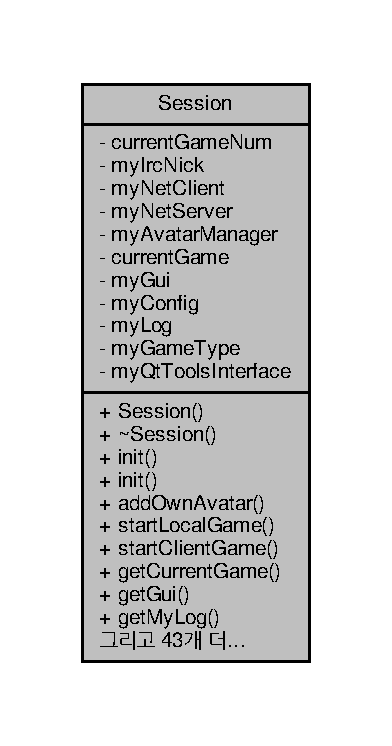
\includegraphics[width=188pt]{class_session__coll__graph}
\end{center}
\end{figure}
\subsection*{Public 타입}
\begin{DoxyCompactItemize}
\item 
enum \hyperlink{class_session_a6989c72d21ad19fd7abbd1c8d95d78c1}{Game\-Type} \{ \hyperlink{class_session_a6989c72d21ad19fd7abbd1c8d95d78c1a9714cf47eacb5ff229c807e48ea68319}{G\-A\-M\-E\-\_\-\-T\-Y\-P\-E\-\_\-\-N\-O\-N\-E}, 
\hyperlink{class_session_a6989c72d21ad19fd7abbd1c8d95d78c1a347a5eef5f0bd9a982bec2ff54a201e7}{G\-A\-M\-E\-\_\-\-T\-Y\-P\-E\-\_\-\-L\-O\-C\-A\-L}, 
\hyperlink{class_session_a6989c72d21ad19fd7abbd1c8d95d78c1a878b602bad23ad76103fb270b21c3a80}{G\-A\-M\-E\-\_\-\-T\-Y\-P\-E\-\_\-\-N\-E\-T\-W\-O\-R\-K}, 
\hyperlink{class_session_a6989c72d21ad19fd7abbd1c8d95d78c1adb35dec5c0038852cb94ffbd5c5739f2}{G\-A\-M\-E\-\_\-\-T\-Y\-P\-E\-\_\-\-I\-N\-T\-E\-R\-N\-E\-T}
 \}
\end{DoxyCompactItemize}
\subsection*{Public 멤버 함수}
\begin{DoxyCompactItemize}
\item 
\hyperlink{class_session_a7bc6792892226050a8cf19d5e9c17541}{Session} (Gui\-Interface $\ast$, Config\-File $\ast$, Log $\ast$)
\item 
\hyperlink{class_session_a8753bb9dee966b7d39abc9b7237cd665}{$\sim$\-Session} ()
\item 
bool \hyperlink{class_session_a94dcf560238662a4e2626a654df008f3}{init} ()
\item 
void \hyperlink{class_session_acb341298736898e0c913aa2e17c819e8}{init} (boost\-::shared\-\_\-ptr$<$ Avatar\-Manager $>$ manager)
\item 
void \hyperlink{class_session_acc80127497f991a082269c2e6b6cddb9}{add\-Own\-Avatar} (const std\-::string \&avatar\-File)
\item 
void \hyperlink{class_session_af2e661d4bcda30cfda7c90547ce2260a}{start\-Local\-Game} (const \hyperlink{struct_game_data}{Game\-Data} \&game\-Data, const \hyperlink{struct_start_data}{Start\-Data} \&start\-Data)
\item 
void \hyperlink{class_session_ae7f595ddf3e73d0d923e9ccd3b77cb56}{start\-Client\-Game} (boost\-::shared\-\_\-ptr$<$ Game $>$ game)
\item 
boost\-::shared\-\_\-ptr$<$ Game $>$ \hyperlink{class_session_a4105c943da66294d2296e31bc34d5ff9}{get\-Current\-Game} ()
\item 
Gui\-Interface $\ast$ \hyperlink{class_session_ab1f394edd6080e4303bd292b0f842ce1}{get\-Gui} ()
\item 
Log $\ast$ \hyperlink{class_session_a8b3eeaaa1732a6a403bf799b8feab70d}{get\-My\-Log} ()
\item 
\hyperlink{class_session_a6989c72d21ad19fd7abbd1c8d95d78c1}{Game\-Type} \hyperlink{class_session_a5e07b844e121855419719abcbd8aa61a}{get\-Game\-Type} ()
\item 
boost\-::shared\-\_\-ptr$<$ Avatar\-Manager $>$ \hyperlink{class_session_a96a5366d8d4455494ca27ed412cb37a5}{get\-Avatar\-Manager} ()
\item 
void \hyperlink{class_session_a2e89781eb6911f3d7a40b475bc83c8c8}{start\-Internet\-Client} ()
\item 
void \hyperlink{class_session_aab2276257cc5c64e11a05784daf414e5}{start\-Network\-Client} (const std\-::string \&server\-Address, unsigned server\-Port, bool ipv6, bool sctp)
\item 
void \hyperlink{class_session_a738cd5d6baccc583228e5bc57d57d80f}{start\-Network\-Client\-For\-Local\-Server} (const \hyperlink{struct_game_data}{Game\-Data} \&game\-Data)
\item 
void \hyperlink{class_session_ad74cf272a2adfaa0a2abcaf31dde167d}{terminate\-Network\-Client} ()
\item 
void \hyperlink{class_session_ae3a49af65eee53bfdb44896ab564458e}{client\-Create\-Game} (const \hyperlink{struct_game_data}{Game\-Data} \&game\-Data, const std\-::string \&name, const std\-::string \&password)
\item 
void \hyperlink{class_session_a4499bc9b022b6af7856ab23ab80d7f99}{client\-Join\-Game} (unsigned game\-Id, const std\-::string \&password)
\item 
void \hyperlink{class_session_a8084d3c69f25fb50c1b42efe07ccbeb7}{client\-Rejoin\-Game} (unsigned game\-Id)
\item 
void \hyperlink{class_session_abf1156cfe81e2786adf7bb369836ca0b}{start\-Network\-Server} (bool dedicated, bool lan\-\_\-local=false)
\item 
void \hyperlink{class_session_afe114af0a76eb150e0aad183eed5b8f1}{send\-Leave\-Current\-Game} ()
\item 
void \hyperlink{class_session_a0b43294e739dab7e8a70c1ed2e852e3d}{send\-Start\-Event} (bool fill\-Up\-With\-Cpu\-Players)
\item 
void \hyperlink{class_session_ab3c9282517142617d9daf5ea08768083}{terminate\-Network\-Server} ()
\item 
bool \hyperlink{class_session_a2277e79b82a29b4ec96aa78e1cb67e7c}{poll\-Network\-Server\-Terminated} ()
\item 
void \hyperlink{class_session_aac851088914580be19d0f9c84698cdb6}{send\-Client\-Player\-Action} ()
\item 
void \hyperlink{class_session_a9e297d28e45b056a09c62ef389308052}{send\-Game\-Chat\-Message} (const std\-::string \&message)
\item 
void \hyperlink{class_session_ae309f290cfefc4c2c145209b7a5a48ff}{send\-Lobby\-Chat\-Message} (const std\-::string \&message)
\item 
void \hyperlink{class_session_a756684d3fb7bc878f39250f5ddd3cc55}{send\-Private\-Chat\-Message} (unsigned target\-Player\-Id, const std\-::string \&message)
\item 
void \hyperlink{class_session_a383cac1e0db6fcbce4d3fa94b3efe9d4}{kick\-Player} (unsigned player\-Id)
\item 
void \hyperlink{class_session_a1a682edf6225afaa72df5f3d17663a35}{kick\-Player} (const std\-::string \&player\-Name)
\item 
void \hyperlink{class_session_aa834f9615a493ae739509e56abab5059}{start\-Vote\-Kick\-Player} (unsigned player\-Id)
\item 
void \hyperlink{class_session_a346c8fa2d61d205f825c2af8a12d2071}{vote\-Kick} (bool do\-Kick)
\item 
void \hyperlink{class_session_a4e99119356023629431163b20e307020}{show\-My\-Cards} ()
\item 
void \hyperlink{class_session_ae23ad66200d0c7ab81f5baddc40ad7ee}{select\-Server} (unsigned server\-Id)
\item 
void \hyperlink{class_session_a111d37566070922bebb97f1c52e811f5}{set\-Login} (const std\-::string \&user\-Name, const std\-::string \&password, bool is\-Guest)
\item 
void \hyperlink{class_session_a2dad06d98159702d5723e895d93cda01}{invite\-Player\-To\-Current\-Game} (unsigned player\-Id)
\item 
void \hyperlink{class_session_aa0083e4f35f82def3c9f05af75449caf}{accept\-Game\-Invitation} (unsigned game\-Id)
\item 
void \hyperlink{class_session_a56768c317805f6fb7f0acded7a703db3}{reject\-Game\-Invitation} (unsigned game\-Id, \hyperlink{game__defs_8h_aa91c16d80068f7d379ed63946b9d9a53}{Deny\-Game\-Invitation\-Reason} reason)
\item 
void \hyperlink{class_session_af1a1915a925b1bc73e5984524d365787}{report\-Bad\-Avatar} (unsigned reported\-Player\-Id, const std\-::string \&avatar\-Hash)
\item 
void \hyperlink{class_session_ab8c30dee4b7dd9d56045caa308bb14d6}{report\-Bad\-Game\-Name} (unsigned game\-Id)
\item 
void \hyperlink{class_session_a1343f531ff9b53c77c873f5034a00a0f}{admin\-Action\-Ban\-Player} (unsigned player\-Id)
\item 
void \hyperlink{class_session_aa772e588d7f1aa1a78ff9633a6cf0e8b}{reset\-Network\-Timeout} ()
\item 
void \hyperlink{class_session_acb24746ea4c50d24d26386e7afb4befa}{admin\-Action\-Close\-Game} (unsigned game\-Id)
\item 
bool \hyperlink{class_session_a7e4c9b0b3bf8f745c22c4f17c365d9ec}{is\-Network\-Client\-Running} () const 
\item 
bool \hyperlink{class_session_a7ac2f5a1bf47626a9b37c739701f84bf}{is\-Network\-Server\-Running} () const 
\item 
\hyperlink{struct_server_info}{Server\-Info} \hyperlink{class_session_a103970a0117442b4db09adaef04847d7}{get\-Client\-Server\-Info} (unsigned server\-Id) const 
\item 
\hyperlink{struct_game_info}{Game\-Info} \hyperlink{class_session_a8f16216769638acec9ce003aca038e67}{get\-Client\-Game\-Info} (unsigned game\-Id) const 
\item 
\hyperlink{struct_player_info}{Player\-Info} \hyperlink{class_session_af0c26f5815db03ddcb83491a080383e3}{get\-Client\-Player\-Info} (unsigned player\-Id) const 
\item 
unsigned \hyperlink{class_session_a4cd156a99a379a966424cfefd93cd31b}{get\-Game\-Id\-Of\-Player} (unsigned player\-Id) const 
\item 
\hyperlink{struct_server_stats}{Server\-Stats} \hyperlink{class_session_aa69deeb42f29e39020a85a7396992925}{get\-Client\-Stats} () const 
\item 
unsigned \hyperlink{class_session_aab5ba527a87413cdeab6a5ea00f4c30d}{get\-Client\-Current\-Game\-Id} () const 
\item 
unsigned \hyperlink{class_session_a82aff275cb035b0440f5139d54338b99}{get\-Client\-Unique\-Player\-Id} () const 
\item 
bool \hyperlink{class_session_aae0e047300fee326aaf11fb060df135e}{get\-Avatar\-File} (const M\-D5\-Buf \&avatar\-M\-D5, std\-::string \&file\-Name)
\end{DoxyCompactItemize}
\subsection*{Private 속성}
\begin{DoxyCompactItemize}
\item 
int \hyperlink{class_session_a89974964b38a285de9ec954b99b0ee3f}{current\-Game\-Num}
\item 
std\-::string \hyperlink{class_session_a95063949539c8584d569d777284784ba}{my\-Irc\-Nick}
\item 
boost\-::shared\-\_\-ptr$<$ Client\-Thread $>$ \hyperlink{class_session_a767e3250d6a14be4c2b86d1e2dfa7b3c}{my\-Net\-Client}
\item 
boost\-::shared\-\_\-ptr$<$ Server\-Manager $>$ \hyperlink{class_session_a0f513f8d52d5026a3c449738da984c29}{my\-Net\-Server}
\item 
boost\-::shared\-\_\-ptr$<$ Avatar\-Manager $>$ \hyperlink{class_session_a53231528d2b4c4babd97c7d1194a5f7e}{my\-Avatar\-Manager}
\item 
boost\-::shared\-\_\-ptr$<$ Game $>$ \hyperlink{class_session_a5c15d5f1be74a30fa167a0af5822113c}{current\-Game}
\item 
Gui\-Interface $\ast$ \hyperlink{class_session_a2725f4b56b109b2e7d75ed780d24fa6d}{my\-Gui}
\item 
Config\-File $\ast$ \hyperlink{class_session_a5bfbe43c623b688e7def57e02704033f}{my\-Config}
\item 
Log $\ast$ \hyperlink{class_session_a1d2dd8533f3c551a5c18211f22d380f8}{my\-Log}
\item 
\hyperlink{class_session_a6989c72d21ad19fd7abbd1c8d95d78c1}{Game\-Type} \hyperlink{class_session_acf11b7b3982bc3e4c5bbf635d5e98496}{my\-Game\-Type}
\item 
Qt\-Tools\-Interface $\ast$ \hyperlink{class_session_a1827a0341223eafa3859f249e73ebd38}{my\-Qt\-Tools\-Interface}
\end{DoxyCompactItemize}


\subsection{멤버 열거형 문서화}
\hypertarget{class_session_a6989c72d21ad19fd7abbd1c8d95d78c1}{\index{Session@{Session}!Game\-Type@{Game\-Type}}
\index{Game\-Type@{Game\-Type}!Session@{Session}}
\subsubsection[{Game\-Type}]{\setlength{\rightskip}{0pt plus 5cm}enum {\bf Session\-::\-Game\-Type}}}\label{class_session_a6989c72d21ad19fd7abbd1c8d95d78c1}
\begin{Desc}
\item[열거형 멤버]\par
\begin{description}
\index{G\-A\-M\-E\-\_\-\-T\-Y\-P\-E\-\_\-\-N\-O\-N\-E@{G\-A\-M\-E\-\_\-\-T\-Y\-P\-E\-\_\-\-N\-O\-N\-E}!Session@{Session}}\index{Session@{Session}!G\-A\-M\-E\-\_\-\-T\-Y\-P\-E\-\_\-\-N\-O\-N\-E@{G\-A\-M\-E\-\_\-\-T\-Y\-P\-E\-\_\-\-N\-O\-N\-E}}\item[{\em 
\hypertarget{class_session_a6989c72d21ad19fd7abbd1c8d95d78c1a9714cf47eacb5ff229c807e48ea68319}{G\-A\-M\-E\-\_\-\-T\-Y\-P\-E\-\_\-\-N\-O\-N\-E}\label{class_session_a6989c72d21ad19fd7abbd1c8d95d78c1a9714cf47eacb5ff229c807e48ea68319}
}]\index{G\-A\-M\-E\-\_\-\-T\-Y\-P\-E\-\_\-\-L\-O\-C\-A\-L@{G\-A\-M\-E\-\_\-\-T\-Y\-P\-E\-\_\-\-L\-O\-C\-A\-L}!Session@{Session}}\index{Session@{Session}!G\-A\-M\-E\-\_\-\-T\-Y\-P\-E\-\_\-\-L\-O\-C\-A\-L@{G\-A\-M\-E\-\_\-\-T\-Y\-P\-E\-\_\-\-L\-O\-C\-A\-L}}\item[{\em 
\hypertarget{class_session_a6989c72d21ad19fd7abbd1c8d95d78c1a347a5eef5f0bd9a982bec2ff54a201e7}{G\-A\-M\-E\-\_\-\-T\-Y\-P\-E\-\_\-\-L\-O\-C\-A\-L}\label{class_session_a6989c72d21ad19fd7abbd1c8d95d78c1a347a5eef5f0bd9a982bec2ff54a201e7}
}]\index{G\-A\-M\-E\-\_\-\-T\-Y\-P\-E\-\_\-\-N\-E\-T\-W\-O\-R\-K@{G\-A\-M\-E\-\_\-\-T\-Y\-P\-E\-\_\-\-N\-E\-T\-W\-O\-R\-K}!Session@{Session}}\index{Session@{Session}!G\-A\-M\-E\-\_\-\-T\-Y\-P\-E\-\_\-\-N\-E\-T\-W\-O\-R\-K@{G\-A\-M\-E\-\_\-\-T\-Y\-P\-E\-\_\-\-N\-E\-T\-W\-O\-R\-K}}\item[{\em 
\hypertarget{class_session_a6989c72d21ad19fd7abbd1c8d95d78c1a878b602bad23ad76103fb270b21c3a80}{G\-A\-M\-E\-\_\-\-T\-Y\-P\-E\-\_\-\-N\-E\-T\-W\-O\-R\-K}\label{class_session_a6989c72d21ad19fd7abbd1c8d95d78c1a878b602bad23ad76103fb270b21c3a80}
}]\index{G\-A\-M\-E\-\_\-\-T\-Y\-P\-E\-\_\-\-I\-N\-T\-E\-R\-N\-E\-T@{G\-A\-M\-E\-\_\-\-T\-Y\-P\-E\-\_\-\-I\-N\-T\-E\-R\-N\-E\-T}!Session@{Session}}\index{Session@{Session}!G\-A\-M\-E\-\_\-\-T\-Y\-P\-E\-\_\-\-I\-N\-T\-E\-R\-N\-E\-T@{G\-A\-M\-E\-\_\-\-T\-Y\-P\-E\-\_\-\-I\-N\-T\-E\-R\-N\-E\-T}}\item[{\em 
\hypertarget{class_session_a6989c72d21ad19fd7abbd1c8d95d78c1adb35dec5c0038852cb94ffbd5c5739f2}{G\-A\-M\-E\-\_\-\-T\-Y\-P\-E\-\_\-\-I\-N\-T\-E\-R\-N\-E\-T}\label{class_session_a6989c72d21ad19fd7abbd1c8d95d78c1adb35dec5c0038852cb94ffbd5c5739f2}
}]\end{description}
\end{Desc}

\begin{DoxyCode}
62 \{ \hyperlink{class_session_a6989c72d21ad19fd7abbd1c8d95d78c1a9714cf47eacb5ff229c807e48ea68319}{GAME\_TYPE\_NONE}, \hyperlink{class_session_a6989c72d21ad19fd7abbd1c8d95d78c1a347a5eef5f0bd9a982bec2ff54a201e7}{GAME\_TYPE\_LOCAL}, 
      \hyperlink{class_session_a6989c72d21ad19fd7abbd1c8d95d78c1a878b602bad23ad76103fb270b21c3a80}{GAME\_TYPE\_NETWORK}, \hyperlink{class_session_a6989c72d21ad19fd7abbd1c8d95d78c1adb35dec5c0038852cb94ffbd5c5739f2}{GAME\_TYPE\_INTERNET} \};
\end{DoxyCode}


\subsection{생성자 \& 소멸자 문서화}
\hypertarget{class_session_a7bc6792892226050a8cf19d5e9c17541}{\index{Session@{Session}!Session@{Session}}
\index{Session@{Session}!Session@{Session}}
\subsubsection[{Session}]{\setlength{\rightskip}{0pt plus 5cm}Session\-::\-Session (
\begin{DoxyParamCaption}
\item[{Gui\-Interface $\ast$}]{g, }
\item[{Config\-File $\ast$}]{c, }
\item[{Log $\ast$}]{l}
\end{DoxyParamCaption}
)}}\label{class_session_a7bc6792892226050a8cf19d5e9c17541}

\begin{DoxyCode}
56     : \hyperlink{class_session_a89974964b38a285de9ec954b99b0ee3f}{currentGameNum}(0), \hyperlink{class_session_a2725f4b56b109b2e7d75ed780d24fa6d}{myGui}(g), \hyperlink{class_session_a5bfbe43c623b688e7def57e02704033f}{myConfig}(c), \hyperlink{class_session_a1d2dd8533f3c551a5c18211f22d380f8}{myLog}(l), 
      \hyperlink{class_session_acf11b7b3982bc3e4c5bbf635d5e98496}{myGameType}(\hyperlink{class_session_a6989c72d21ad19fd7abbd1c8d95d78c1a9714cf47eacb5ff229c807e48ea68319}{GAME\_TYPE\_NONE})
57 \{
58     \hyperlink{class_session_a1827a0341223eafa3859f249e73ebd38}{myQtToolsInterface} = CreateQtToolsWrapper();
59 \}
\end{DoxyCode}
\hypertarget{class_session_a8753bb9dee966b7d39abc9b7237cd665}{\index{Session@{Session}!$\sim$\-Session@{$\sim$\-Session}}
\index{$\sim$\-Session@{$\sim$\-Session}!Session@{Session}}
\subsubsection[{$\sim$\-Session}]{\setlength{\rightskip}{0pt plus 5cm}Session\-::$\sim$\-Session (
\begin{DoxyParamCaption}
{}
\end{DoxyParamCaption}
)}}\label{class_session_a8753bb9dee966b7d39abc9b7237cd665}

\begin{DoxyCode}
63 \{
64     \hyperlink{class_session_ad74cf272a2adfaa0a2abcaf31dde167d}{terminateNetworkClient}();
65     \hyperlink{class_session_ab3c9282517142617d9daf5ea08768083}{terminateNetworkServer}();
66     \textcolor{keyword}{delete} \hyperlink{class_session_a1827a0341223eafa3859f249e73ebd38}{myQtToolsInterface};
67     \hyperlink{class_session_a1827a0341223eafa3859f249e73ebd38}{myQtToolsInterface} = 0;
68     \textcolor{keyword}{delete} \hyperlink{class_session_a1d2dd8533f3c551a5c18211f22d380f8}{myLog};
69     \hyperlink{class_session_a1d2dd8533f3c551a5c18211f22d380f8}{myLog} = 0;
70 \}
\end{DoxyCode}


이 함수 내부에서 호출하는 함수들에 대한 그래프입니다.\-:\nopagebreak
\begin{figure}[H]
\begin{center}
\leavevmode
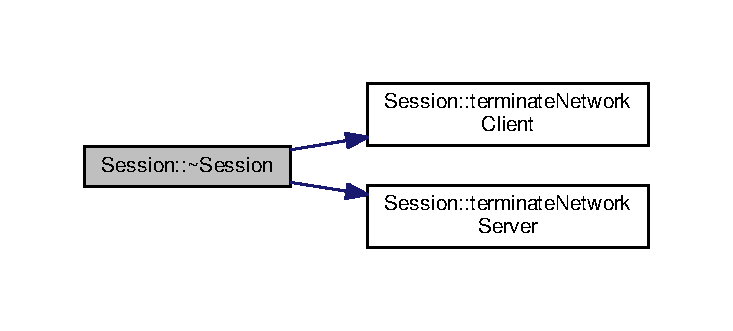
\includegraphics[width=350pt]{class_session_a8753bb9dee966b7d39abc9b7237cd665_cgraph}
\end{center}
\end{figure}




\subsection{멤버 함수 문서화}
\hypertarget{class_session_aa0083e4f35f82def3c9f05af75449caf}{\index{Session@{Session}!accept\-Game\-Invitation@{accept\-Game\-Invitation}}
\index{accept\-Game\-Invitation@{accept\-Game\-Invitation}!Session@{Session}}
\subsubsection[{accept\-Game\-Invitation}]{\setlength{\rightskip}{0pt plus 5cm}void Session\-::accept\-Game\-Invitation (
\begin{DoxyParamCaption}
\item[{unsigned}]{game\-Id}
\end{DoxyParamCaption}
)}}\label{class_session_aa0083e4f35f82def3c9f05af75449caf}

\begin{DoxyCode}
489 \{
490     \textcolor{keywordflow}{if} (!\hyperlink{class_session_a767e3250d6a14be4c2b86d1e2dfa7b3c}{myNetClient})
491         \textcolor{keywordflow}{return}; \textcolor{comment}{// only act if client is running.}
492     \hyperlink{class_session_a767e3250d6a14be4c2b86d1e2dfa7b3c}{myNetClient}->SendJoinGame(
493         gameId,
494         \textcolor{stringliteral}{""},
495         \hyperlink{class_session_a5bfbe43c623b688e7def57e02704033f}{myConfig}->readConfigInt(\textcolor{stringliteral}{"NetAutoLeaveGameAfterFinish"}) == 1
496     );
497 \}
\end{DoxyCode}
\hypertarget{class_session_acc80127497f991a082269c2e6b6cddb9}{\index{Session@{Session}!add\-Own\-Avatar@{add\-Own\-Avatar}}
\index{add\-Own\-Avatar@{add\-Own\-Avatar}!Session@{Session}}
\subsubsection[{add\-Own\-Avatar}]{\setlength{\rightskip}{0pt plus 5cm}void Session\-::add\-Own\-Avatar (
\begin{DoxyParamCaption}
\item[{const std\-::string \&}]{avatar\-File}
\end{DoxyParamCaption}
)}}\label{class_session_acc80127497f991a082269c2e6b6cddb9}

\begin{DoxyCode}
96 \{
97     \hyperlink{class_session_a53231528d2b4c4babd97c7d1194a5f7e}{myAvatarManager}->AddSingleAvatar(avatarFile);
98 \}
\end{DoxyCode}


이 함수를 호출하는 함수들에 대한 그래프입니다.\-:\nopagebreak
\begin{figure}[H]
\begin{center}
\leavevmode
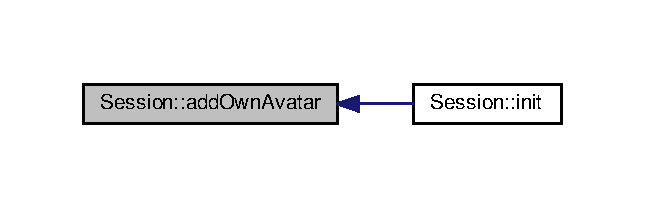
\includegraphics[width=310pt]{class_session_acc80127497f991a082269c2e6b6cddb9_icgraph}
\end{center}
\end{figure}


\hypertarget{class_session_a1343f531ff9b53c77c873f5034a00a0f}{\index{Session@{Session}!admin\-Action\-Ban\-Player@{admin\-Action\-Ban\-Player}}
\index{admin\-Action\-Ban\-Player@{admin\-Action\-Ban\-Player}!Session@{Session}}
\subsubsection[{admin\-Action\-Ban\-Player}]{\setlength{\rightskip}{0pt plus 5cm}void Session\-::admin\-Action\-Ban\-Player (
\begin{DoxyParamCaption}
\item[{unsigned}]{player\-Id}
\end{DoxyParamCaption}
)}}\label{class_session_a1343f531ff9b53c77c873f5034a00a0f}

\begin{DoxyCode}
442 \{
443     \textcolor{keywordflow}{if} (!\hyperlink{class_session_a767e3250d6a14be4c2b86d1e2dfa7b3c}{myNetClient})
444         \textcolor{keywordflow}{return}; \textcolor{comment}{// only act if client is running.}
445     \hyperlink{class_session_a767e3250d6a14be4c2b86d1e2dfa7b3c}{myNetClient}->SendAdminBanPlayer(playerId);
446 \}
\end{DoxyCode}
\hypertarget{class_session_acb24746ea4c50d24d26386e7afb4befa}{\index{Session@{Session}!admin\-Action\-Close\-Game@{admin\-Action\-Close\-Game}}
\index{admin\-Action\-Close\-Game@{admin\-Action\-Close\-Game}!Session@{Session}}
\subsubsection[{admin\-Action\-Close\-Game}]{\setlength{\rightskip}{0pt plus 5cm}void Session\-::admin\-Action\-Close\-Game (
\begin{DoxyParamCaption}
\item[{unsigned}]{game\-Id}
\end{DoxyParamCaption}
)}}\label{class_session_acb24746ea4c50d24d26386e7afb4befa}

\begin{DoxyCode}
435 \{
436     \textcolor{keywordflow}{if} (!\hyperlink{class_session_a767e3250d6a14be4c2b86d1e2dfa7b3c}{myNetClient})
437         \textcolor{keywordflow}{return}; \textcolor{comment}{// only act if client is running.}
438     \hyperlink{class_session_a767e3250d6a14be4c2b86d1e2dfa7b3c}{myNetClient}->SendAdminRemoveGame(gameId);
439 \}
\end{DoxyCode}
\hypertarget{class_session_ae3a49af65eee53bfdb44896ab564458e}{\index{Session@{Session}!client\-Create\-Game@{client\-Create\-Game}}
\index{client\-Create\-Game@{client\-Create\-Game}!Session@{Session}}
\subsubsection[{client\-Create\-Game}]{\setlength{\rightskip}{0pt plus 5cm}void Session\-::client\-Create\-Game (
\begin{DoxyParamCaption}
\item[{const {\bf Game\-Data} \&}]{game\-Data, }
\item[{const std\-::string \&}]{name, }
\item[{const std\-::string \&}]{password}
\end{DoxyParamCaption}
)}}\label{class_session_ae3a49af65eee53bfdb44896ab564458e}

\begin{DoxyCode}
281 \{
282     \textcolor{keywordflow}{if} (!\hyperlink{class_session_a767e3250d6a14be4c2b86d1e2dfa7b3c}{myNetClient})
283         \textcolor{keywordflow}{return}; \textcolor{comment}{// only act if client is running.}
284     \hyperlink{class_session_a767e3250d6a14be4c2b86d1e2dfa7b3c}{myNetClient}->SendCreateGame(
285         gameData,
286         name,
287         password,
288         \hyperlink{class_session_a5bfbe43c623b688e7def57e02704033f}{myConfig}->readConfigInt(\textcolor{stringliteral}{"NetAutoLeaveGameAfterFinish"}) == 1
289     );
290 \}
\end{DoxyCode}
\hypertarget{class_session_a4499bc9b022b6af7856ab23ab80d7f99}{\index{Session@{Session}!client\-Join\-Game@{client\-Join\-Game}}
\index{client\-Join\-Game@{client\-Join\-Game}!Session@{Session}}
\subsubsection[{client\-Join\-Game}]{\setlength{\rightskip}{0pt plus 5cm}void Session\-::client\-Join\-Game (
\begin{DoxyParamCaption}
\item[{unsigned}]{game\-Id, }
\item[{const std\-::string \&}]{password}
\end{DoxyParamCaption}
)}}\label{class_session_a4499bc9b022b6af7856ab23ab80d7f99}

\begin{DoxyCode}
293 \{
294     \textcolor{keywordflow}{if} (!\hyperlink{class_session_a767e3250d6a14be4c2b86d1e2dfa7b3c}{myNetClient})
295         \textcolor{keywordflow}{return}; \textcolor{comment}{// only act if client is running.}
296     \hyperlink{class_session_a767e3250d6a14be4c2b86d1e2dfa7b3c}{myNetClient}->SendJoinGame(
297         gameId,
298         password,
299         \hyperlink{class_session_a5bfbe43c623b688e7def57e02704033f}{myConfig}->readConfigInt(\textcolor{stringliteral}{"NetAutoLeaveGameAfterFinish"}) == 1
300     );
301 \}
\end{DoxyCode}
\hypertarget{class_session_a8084d3c69f25fb50c1b42efe07ccbeb7}{\index{Session@{Session}!client\-Rejoin\-Game@{client\-Rejoin\-Game}}
\index{client\-Rejoin\-Game@{client\-Rejoin\-Game}!Session@{Session}}
\subsubsection[{client\-Rejoin\-Game}]{\setlength{\rightskip}{0pt plus 5cm}void Session\-::client\-Rejoin\-Game (
\begin{DoxyParamCaption}
\item[{unsigned}]{game\-Id}
\end{DoxyParamCaption}
)}}\label{class_session_a8084d3c69f25fb50c1b42efe07ccbeb7}

\begin{DoxyCode}
304 \{
305     \textcolor{keywordflow}{if} (!\hyperlink{class_session_a767e3250d6a14be4c2b86d1e2dfa7b3c}{myNetClient})
306         \textcolor{keywordflow}{return}; \textcolor{comment}{// only act if client is running.}
307     \hyperlink{class_session_a767e3250d6a14be4c2b86d1e2dfa7b3c}{myNetClient}->SendRejoinGame(
308         gameId,
309         \hyperlink{class_session_a5bfbe43c623b688e7def57e02704033f}{myConfig}->readConfigInt(\textcolor{stringliteral}{"NetAutoLeaveGameAfterFinish"}) == 1
310     );
311 \}
\end{DoxyCode}
\hypertarget{class_session_aae0e047300fee326aaf11fb060df135e}{\index{Session@{Session}!get\-Avatar\-File@{get\-Avatar\-File}}
\index{get\-Avatar\-File@{get\-Avatar\-File}!Session@{Session}}
\subsubsection[{get\-Avatar\-File}]{\setlength{\rightskip}{0pt plus 5cm}bool Session\-::get\-Avatar\-File (
\begin{DoxyParamCaption}
\item[{const M\-D5\-Buf \&}]{avatar\-M\-D5, }
\item[{std\-::string \&}]{file\-Name}
\end{DoxyParamCaption}
)}}\label{class_session_aae0e047300fee326aaf11fb060df135e}

\begin{DoxyCode}
604 \{
605     \textcolor{keywordtype}{bool} retVal = \textcolor{keyword}{false};
606     \textcolor{keywordflow}{if} (\hyperlink{class_session_a53231528d2b4c4babd97c7d1194a5f7e}{myAvatarManager}.get()) \{
607         \textcolor{keywordtype}{string} tmpFileName;
608         retVal = \hyperlink{class_session_a53231528d2b4c4babd97c7d1194a5f7e}{myAvatarManager}->GetAvatarFileName(avatarMD5, tmpFileName);
609         \textcolor{keywordflow}{if} (retVal)
610             fileName = \hyperlink{class_session_a1827a0341223eafa3859f249e73ebd38}{myQtToolsInterface}->stringToUtf8(tmpFileName);
611     \}
612     \textcolor{keywordflow}{return} retVal;
613 \}\end{DoxyCode}
\hypertarget{class_session_a96a5366d8d4455494ca27ed412cb37a5}{\index{Session@{Session}!get\-Avatar\-Manager@{get\-Avatar\-Manager}}
\index{get\-Avatar\-Manager@{get\-Avatar\-Manager}!Session@{Session}}
\subsubsection[{get\-Avatar\-Manager}]{\setlength{\rightskip}{0pt plus 5cm}boost\-::shared\-\_\-ptr$<$ Avatar\-Manager $>$ Session\-::get\-Avatar\-Manager (
\begin{DoxyParamCaption}
{}
\end{DoxyParamCaption}
)}}\label{class_session_a96a5366d8d4455494ca27ed412cb37a5}

\begin{DoxyCode}
175 \{
176     \textcolor{keywordflow}{return} \hyperlink{class_session_a53231528d2b4c4babd97c7d1194a5f7e}{myAvatarManager};
177 \}
\end{DoxyCode}
\hypertarget{class_session_aab5ba527a87413cdeab6a5ea00f4c30d}{\index{Session@{Session}!get\-Client\-Current\-Game\-Id@{get\-Client\-Current\-Game\-Id}}
\index{get\-Client\-Current\-Game\-Id@{get\-Client\-Current\-Game\-Id}!Session@{Session}}
\subsubsection[{get\-Client\-Current\-Game\-Id}]{\setlength{\rightskip}{0pt plus 5cm}unsigned Session\-::get\-Client\-Current\-Game\-Id (
\begin{DoxyParamCaption}
{}
\end{DoxyParamCaption}
) const}}\label{class_session_aab5ba527a87413cdeab6a5ea00f4c30d}

\begin{DoxyCode}
588 \{
589     \textcolor{keywordtype}{unsigned} \textcolor{keywordtype}{id} = 0;
590     \textcolor{keywordflow}{if} (\hyperlink{class_session_a767e3250d6a14be4c2b86d1e2dfa7b3c}{myNetClient})
591         \textcolor{keywordtype}{id} = \hyperlink{class_session_a767e3250d6a14be4c2b86d1e2dfa7b3c}{myNetClient}->GetGameId();
592     \textcolor{keywordflow}{return} id;
593 \}
\end{DoxyCode}
\hypertarget{class_session_a8f16216769638acec9ce003aca038e67}{\index{Session@{Session}!get\-Client\-Game\-Info@{get\-Client\-Game\-Info}}
\index{get\-Client\-Game\-Info@{get\-Client\-Game\-Info}!Session@{Session}}
\subsubsection[{get\-Client\-Game\-Info}]{\setlength{\rightskip}{0pt plus 5cm}{\bf Game\-Info} Session\-::get\-Client\-Game\-Info (
\begin{DoxyParamCaption}
\item[{unsigned}]{game\-Id}
\end{DoxyParamCaption}
) const}}\label{class_session_a8f16216769638acec9ce003aca038e67}

\begin{DoxyCode}
556 \{
557     \hyperlink{struct_game_info}{GameInfo} info;
558     \textcolor{keywordflow}{if} (\hyperlink{class_session_a767e3250d6a14be4c2b86d1e2dfa7b3c}{myNetClient})
559         info = \hyperlink{class_session_a767e3250d6a14be4c2b86d1e2dfa7b3c}{myNetClient}->GetGameInfo(playerId);
560     \textcolor{keywordflow}{return} info;
561 \}
\end{DoxyCode}
\hypertarget{class_session_af0c26f5815db03ddcb83491a080383e3}{\index{Session@{Session}!get\-Client\-Player\-Info@{get\-Client\-Player\-Info}}
\index{get\-Client\-Player\-Info@{get\-Client\-Player\-Info}!Session@{Session}}
\subsubsection[{get\-Client\-Player\-Info}]{\setlength{\rightskip}{0pt plus 5cm}{\bf Player\-Info} Session\-::get\-Client\-Player\-Info (
\begin{DoxyParamCaption}
\item[{unsigned}]{player\-Id}
\end{DoxyParamCaption}
) const}}\label{class_session_af0c26f5815db03ddcb83491a080383e3}

\begin{DoxyCode}
564 \{
565     \hyperlink{struct_player_info}{PlayerInfo} info;
566     \textcolor{keywordflow}{if} (\hyperlink{class_session_a767e3250d6a14be4c2b86d1e2dfa7b3c}{myNetClient})
567         info = \hyperlink{class_session_a767e3250d6a14be4c2b86d1e2dfa7b3c}{myNetClient}->GetPlayerInfo(playerId);
568     \textcolor{keywordflow}{return} info;
569 \}
\end{DoxyCode}
\hypertarget{class_session_a103970a0117442b4db09adaef04847d7}{\index{Session@{Session}!get\-Client\-Server\-Info@{get\-Client\-Server\-Info}}
\index{get\-Client\-Server\-Info@{get\-Client\-Server\-Info}!Session@{Session}}
\subsubsection[{get\-Client\-Server\-Info}]{\setlength{\rightskip}{0pt plus 5cm}{\bf Server\-Info} Session\-::get\-Client\-Server\-Info (
\begin{DoxyParamCaption}
\item[{unsigned}]{server\-Id}
\end{DoxyParamCaption}
) const}}\label{class_session_a103970a0117442b4db09adaef04847d7}

\begin{DoxyCode}
548 \{
549     \hyperlink{struct_server_info}{ServerInfo} info;
550     \textcolor{keywordflow}{if} (\hyperlink{class_session_a767e3250d6a14be4c2b86d1e2dfa7b3c}{myNetClient})
551         info = \hyperlink{class_session_a767e3250d6a14be4c2b86d1e2dfa7b3c}{myNetClient}->GetServerInfo(serverId);
552     \textcolor{keywordflow}{return} info;
553 \}
\end{DoxyCode}
\hypertarget{class_session_aa69deeb42f29e39020a85a7396992925}{\index{Session@{Session}!get\-Client\-Stats@{get\-Client\-Stats}}
\index{get\-Client\-Stats@{get\-Client\-Stats}!Session@{Session}}
\subsubsection[{get\-Client\-Stats}]{\setlength{\rightskip}{0pt plus 5cm}{\bf Server\-Stats} Session\-::get\-Client\-Stats (
\begin{DoxyParamCaption}
{}
\end{DoxyParamCaption}
) const}}\label{class_session_aa69deeb42f29e39020a85a7396992925}

\begin{DoxyCode}
580 \{
581     \hyperlink{struct_server_stats}{ServerStats} stats;
582     \textcolor{keywordflow}{if} (\hyperlink{class_session_a767e3250d6a14be4c2b86d1e2dfa7b3c}{myNetClient})
583         stats = \hyperlink{class_session_a767e3250d6a14be4c2b86d1e2dfa7b3c}{myNetClient}->GetStatData();
584     \textcolor{keywordflow}{return} stats;
585 \}
\end{DoxyCode}
\hypertarget{class_session_a82aff275cb035b0440f5139d54338b99}{\index{Session@{Session}!get\-Client\-Unique\-Player\-Id@{get\-Client\-Unique\-Player\-Id}}
\index{get\-Client\-Unique\-Player\-Id@{get\-Client\-Unique\-Player\-Id}!Session@{Session}}
\subsubsection[{get\-Client\-Unique\-Player\-Id}]{\setlength{\rightskip}{0pt plus 5cm}unsigned Session\-::get\-Client\-Unique\-Player\-Id (
\begin{DoxyParamCaption}
{}
\end{DoxyParamCaption}
) const}}\label{class_session_a82aff275cb035b0440f5139d54338b99}

\begin{DoxyCode}
596 \{
597     \textcolor{keywordtype}{unsigned} \textcolor{keywordtype}{id} = 0;
598     \textcolor{keywordflow}{if} (\hyperlink{class_session_a767e3250d6a14be4c2b86d1e2dfa7b3c}{myNetClient})
599         \textcolor{keywordtype}{id} = \hyperlink{class_session_a767e3250d6a14be4c2b86d1e2dfa7b3c}{myNetClient}->GetGuiPlayerId();
600     \textcolor{keywordflow}{return} id;
601 \}
\end{DoxyCode}
\hypertarget{class_session_a4105c943da66294d2296e31bc34d5ff9}{\index{Session@{Session}!get\-Current\-Game@{get\-Current\-Game}}
\index{get\-Current\-Game@{get\-Current\-Game}!Session@{Session}}
\subsubsection[{get\-Current\-Game}]{\setlength{\rightskip}{0pt plus 5cm}boost\-::shared\-\_\-ptr$<$ Game $>$ Session\-::get\-Current\-Game (
\begin{DoxyParamCaption}
{}
\end{DoxyParamCaption}
)}}\label{class_session_a4105c943da66294d2296e31bc34d5ff9}

\begin{DoxyCode}
160 \{
161     \textcolor{keywordflow}{return} \hyperlink{class_session_a5c15d5f1be74a30fa167a0af5822113c}{currentGame};
162 \}
\end{DoxyCode}
\hypertarget{class_session_a4cd156a99a379a966424cfefd93cd31b}{\index{Session@{Session}!get\-Game\-Id\-Of\-Player@{get\-Game\-Id\-Of\-Player}}
\index{get\-Game\-Id\-Of\-Player@{get\-Game\-Id\-Of\-Player}!Session@{Session}}
\subsubsection[{get\-Game\-Id\-Of\-Player}]{\setlength{\rightskip}{0pt plus 5cm}unsigned Session\-::get\-Game\-Id\-Of\-Player (
\begin{DoxyParamCaption}
\item[{unsigned}]{player\-Id}
\end{DoxyParamCaption}
) const}}\label{class_session_a4cd156a99a379a966424cfefd93cd31b}

\begin{DoxyCode}
572 \{
573     \textcolor{keywordtype}{unsigned} gameId = 0;
574     \textcolor{keywordflow}{if} (\hyperlink{class_session_a767e3250d6a14be4c2b86d1e2dfa7b3c}{myNetClient})
575         gameId = \hyperlink{class_session_a767e3250d6a14be4c2b86d1e2dfa7b3c}{myNetClient}->GetGameIdOfPlayer(playerId);
576     \textcolor{keywordflow}{return} gameId;
577 \}
\end{DoxyCode}
\hypertarget{class_session_a5e07b844e121855419719abcbd8aa61a}{\index{Session@{Session}!get\-Game\-Type@{get\-Game\-Type}}
\index{get\-Game\-Type@{get\-Game\-Type}!Session@{Session}}
\subsubsection[{get\-Game\-Type}]{\setlength{\rightskip}{0pt plus 5cm}{\bf Session\-::\-Game\-Type} Session\-::get\-Game\-Type (
\begin{DoxyParamCaption}
{}
\end{DoxyParamCaption}
)}}\label{class_session_a5e07b844e121855419719abcbd8aa61a}

\begin{DoxyCode}
170 \{
171     \textcolor{keywordflow}{return} \hyperlink{class_session_acf11b7b3982bc3e4c5bbf635d5e98496}{myGameType};
172 \}
\end{DoxyCode}
\hypertarget{class_session_ab1f394edd6080e4303bd292b0f842ce1}{\index{Session@{Session}!get\-Gui@{get\-Gui}}
\index{get\-Gui@{get\-Gui}!Session@{Session}}
\subsubsection[{get\-Gui}]{\setlength{\rightskip}{0pt plus 5cm}Gui\-Interface $\ast$ Session\-::get\-Gui (
\begin{DoxyParamCaption}
{}
\end{DoxyParamCaption}
)}}\label{class_session_ab1f394edd6080e4303bd292b0f842ce1}

\begin{DoxyCode}
165 \{
166     \textcolor{keywordflow}{return} \hyperlink{class_session_a2725f4b56b109b2e7d75ed780d24fa6d}{myGui};
167 \}
\end{DoxyCode}
\hypertarget{class_session_a8b3eeaaa1732a6a403bf799b8feab70d}{\index{Session@{Session}!get\-My\-Log@{get\-My\-Log}}
\index{get\-My\-Log@{get\-My\-Log}!Session@{Session}}
\subsubsection[{get\-My\-Log}]{\setlength{\rightskip}{0pt plus 5cm}Log$\ast$ Session\-::get\-My\-Log (
\begin{DoxyParamCaption}
{}
\end{DoxyParamCaption}
)\hspace{0.3cm}{\ttfamily [inline]}}}\label{class_session_a8b3eeaaa1732a6a403bf799b8feab70d}

\begin{DoxyCode}
76                     \{
77         \textcolor{keywordflow}{return} \hyperlink{class_session_a1d2dd8533f3c551a5c18211f22d380f8}{myLog};
78     \}
\end{DoxyCode}
\hypertarget{class_session_a94dcf560238662a4e2626a654df008f3}{\index{Session@{Session}!init@{init}}
\index{init@{init}!Session@{Session}}
\subsubsection[{init}]{\setlength{\rightskip}{0pt plus 5cm}bool Session\-::init (
\begin{DoxyParamCaption}
{}
\end{DoxyParamCaption}
)}}\label{class_session_a94dcf560238662a4e2626a654df008f3}

\begin{DoxyCode}
73 \{
74     \hyperlink{class_session_a53231528d2b4c4babd97c7d1194a5f7e}{myAvatarManager}.reset(\textcolor{keyword}{new} AvatarManager(
75                               \hyperlink{class_session_a5bfbe43c623b688e7def57e02704033f}{myConfig}->readConfigInt(\textcolor{stringliteral}{"ServerUsePutAvatars"}) == 1,
76                               \hyperlink{class_session_a5bfbe43c623b688e7def57e02704033f}{myConfig}->readConfigString(\textcolor{stringliteral}{"ServerPutAvatarsAddress"}),
77                               \hyperlink{class_session_a5bfbe43c623b688e7def57e02704033f}{myConfig}->readConfigString(\textcolor{stringliteral}{"ServerPutAvatarsUser"}),
78                               \hyperlink{class_session_a5bfbe43c623b688e7def57e02704033f}{myConfig}->readConfigString(\textcolor{stringliteral}{"ServerPutAvatarsPassword"})
79                           ));
80     \textcolor{keywordtype}{bool} retVal = \hyperlink{class_session_a53231528d2b4c4babd97c7d1194a5f7e}{myAvatarManager}->Init(
81                       \hyperlink{class_session_a1827a0341223eafa3859f249e73ebd38}{myQtToolsInterface}->stringFromUtf8(
      \hyperlink{class_session_a5bfbe43c623b688e7def57e02704033f}{myConfig}->readConfigString(\textcolor{stringliteral}{"AppDataDir"})),
82                       \hyperlink{class_session_a1827a0341223eafa3859f249e73ebd38}{myQtToolsInterface}->stringFromUtf8(
      \hyperlink{class_session_a5bfbe43c623b688e7def57e02704033f}{myConfig}->readConfigString(\textcolor{stringliteral}{"CacheDir"})));
83     \hyperlink{class_session_acc80127497f991a082269c2e6b6cddb9}{addOwnAvatar}(\hyperlink{class_session_a1827a0341223eafa3859f249e73ebd38}{myQtToolsInterface}->stringFromUtf8(
      \hyperlink{class_session_a5bfbe43c623b688e7def57e02704033f}{myConfig}->readConfigString(\textcolor{stringliteral}{"MyAvatar"})));
84 \textcolor{preprocessor}{#ifndef POKERTH\_OFFICIAL\_SERVER
}
85 \textcolor{preprocessor}{}    \hyperlink{class_session_a53231528d2b4c4babd97c7d1194a5f7e}{myAvatarManager}->RemoveOldAvatarCacheEntries();
86 \textcolor{preprocessor}{#endif
}
87 \textcolor{preprocessor}{}    \textcolor{keywordflow}{return} retVal;
88 \}
\end{DoxyCode}


이 함수 내부에서 호출하는 함수들에 대한 그래프입니다.\-:\nopagebreak
\begin{figure}[H]
\begin{center}
\leavevmode
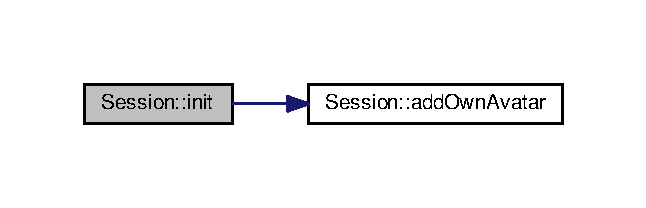
\includegraphics[width=310pt]{class_session_a94dcf560238662a4e2626a654df008f3_cgraph}
\end{center}
\end{figure}


\hypertarget{class_session_acb341298736898e0c913aa2e17c819e8}{\index{Session@{Session}!init@{init}}
\index{init@{init}!Session@{Session}}
\subsubsection[{init}]{\setlength{\rightskip}{0pt plus 5cm}void Session\-::init (
\begin{DoxyParamCaption}
\item[{boost\-::shared\-\_\-ptr$<$ Avatar\-Manager $>$}]{manager}
\end{DoxyParamCaption}
)}}\label{class_session_acb341298736898e0c913aa2e17c819e8}

\begin{DoxyCode}
91 \{
92     \hyperlink{class_session_a53231528d2b4c4babd97c7d1194a5f7e}{myAvatarManager} = manager;
93 \}
\end{DoxyCode}
\hypertarget{class_session_a2dad06d98159702d5723e895d93cda01}{\index{Session@{Session}!invite\-Player\-To\-Current\-Game@{invite\-Player\-To\-Current\-Game}}
\index{invite\-Player\-To\-Current\-Game@{invite\-Player\-To\-Current\-Game}!Session@{Session}}
\subsubsection[{invite\-Player\-To\-Current\-Game}]{\setlength{\rightskip}{0pt plus 5cm}void Session\-::invite\-Player\-To\-Current\-Game (
\begin{DoxyParamCaption}
\item[{unsigned}]{player\-Id}
\end{DoxyParamCaption}
)}}\label{class_session_a2dad06d98159702d5723e895d93cda01}

\begin{DoxyCode}
481 \{
482     \textcolor{keywordflow}{if} (!\hyperlink{class_session_a767e3250d6a14be4c2b86d1e2dfa7b3c}{myNetClient})
483         \textcolor{keywordflow}{return}; \textcolor{comment}{// only act if client is running.}
484     \hyperlink{class_session_a767e3250d6a14be4c2b86d1e2dfa7b3c}{myNetClient}->SendInvitePlayerToCurrentGame(playerId);
485 \}
\end{DoxyCode}
\hypertarget{class_session_a7e4c9b0b3bf8f745c22c4f17c365d9ec}{\index{Session@{Session}!is\-Network\-Client\-Running@{is\-Network\-Client\-Running}}
\index{is\-Network\-Client\-Running@{is\-Network\-Client\-Running}!Session@{Session}}
\subsubsection[{is\-Network\-Client\-Running}]{\setlength{\rightskip}{0pt plus 5cm}bool Session\-::is\-Network\-Client\-Running (
\begin{DoxyParamCaption}
{}
\end{DoxyParamCaption}
) const}}\label{class_session_a7e4c9b0b3bf8f745c22c4f17c365d9ec}

\begin{DoxyCode}
536 \{
537     \textcolor{comment}{// This, and every place which calls this, is a HACK.}
538     \textcolor{keywordflow}{return} \hyperlink{class_session_a767e3250d6a14be4c2b86d1e2dfa7b3c}{myNetClient}.get() != NULL;
539 \}
\end{DoxyCode}
\hypertarget{class_session_a7ac2f5a1bf47626a9b37c739701f84bf}{\index{Session@{Session}!is\-Network\-Server\-Running@{is\-Network\-Server\-Running}}
\index{is\-Network\-Server\-Running@{is\-Network\-Server\-Running}!Session@{Session}}
\subsubsection[{is\-Network\-Server\-Running}]{\setlength{\rightskip}{0pt plus 5cm}bool Session\-::is\-Network\-Server\-Running (
\begin{DoxyParamCaption}
{}
\end{DoxyParamCaption}
) const}}\label{class_session_a7ac2f5a1bf47626a9b37c739701f84bf}

\begin{DoxyCode}
542 \{
543     \textcolor{comment}{// This, and every place which calls this, is a HACK.}
544     \textcolor{keywordflow}{return} \hyperlink{class_session_a0f513f8d52d5026a3c449738da984c29}{myNetServer}.get() != NULL;
545 \}
\end{DoxyCode}
\hypertarget{class_session_a383cac1e0db6fcbce4d3fa94b3efe9d4}{\index{Session@{Session}!kick\-Player@{kick\-Player}}
\index{kick\-Player@{kick\-Player}!Session@{Session}}
\subsubsection[{kick\-Player}]{\setlength{\rightskip}{0pt plus 5cm}void Session\-::kick\-Player (
\begin{DoxyParamCaption}
\item[{unsigned}]{player\-Id}
\end{DoxyParamCaption}
)}}\label{class_session_a383cac1e0db6fcbce4d3fa94b3efe9d4}

\begin{DoxyCode}
421 \{
422     \textcolor{keywordflow}{if} (!\hyperlink{class_session_a767e3250d6a14be4c2b86d1e2dfa7b3c}{myNetClient})
423         \textcolor{keywordflow}{return}; \textcolor{comment}{// only act if client is running.}
424     \hyperlink{class_session_a767e3250d6a14be4c2b86d1e2dfa7b3c}{myNetClient}->SendKickPlayer(playerId);
425 \}
\end{DoxyCode}
\hypertarget{class_session_a1a682edf6225afaa72df5f3d17663a35}{\index{Session@{Session}!kick\-Player@{kick\-Player}}
\index{kick\-Player@{kick\-Player}!Session@{Session}}
\subsubsection[{kick\-Player}]{\setlength{\rightskip}{0pt plus 5cm}void Session\-::kick\-Player (
\begin{DoxyParamCaption}
\item[{const std\-::string \&}]{player\-Name}
\end{DoxyParamCaption}
)}}\label{class_session_a1a682edf6225afaa72df5f3d17663a35}
\hypertarget{class_session_a2277e79b82a29b4ec96aa78e1cb67e7c}{\index{Session@{Session}!poll\-Network\-Server\-Terminated@{poll\-Network\-Server\-Terminated}}
\index{poll\-Network\-Server\-Terminated@{poll\-Network\-Server\-Terminated}!Session@{Session}}
\subsubsection[{poll\-Network\-Server\-Terminated}]{\setlength{\rightskip}{0pt plus 5cm}bool Session\-::poll\-Network\-Server\-Terminated (
\begin{DoxyParamCaption}
{}
\end{DoxyParamCaption}
)}}\label{class_session_a2277e79b82a29b4ec96aa78e1cb67e7c}

\begin{DoxyCode}
366 \{
367     \textcolor{keywordtype}{bool} retVal = \textcolor{keyword}{false};
368     \textcolor{keywordflow}{if} (!\hyperlink{class_session_a0f513f8d52d5026a3c449738da984c29}{myNetServer})
369         retVal = \textcolor{keyword}{true}; \textcolor{comment}{// already terminated}
370     \textcolor{keywordflow}{else} \{
371         \textcolor{keywordflow}{if} (\hyperlink{class_session_a0f513f8d52d5026a3c449738da984c29}{myNetServer}->JoinAll(\textcolor{keyword}{false}))
372             retVal = \textcolor{keyword}{true};
373     \}
374     \textcolor{keywordflow}{return} retVal;
375 \}
\end{DoxyCode}
\hypertarget{class_session_a56768c317805f6fb7f0acded7a703db3}{\index{Session@{Session}!reject\-Game\-Invitation@{reject\-Game\-Invitation}}
\index{reject\-Game\-Invitation@{reject\-Game\-Invitation}!Session@{Session}}
\subsubsection[{reject\-Game\-Invitation}]{\setlength{\rightskip}{0pt plus 5cm}void Session\-::reject\-Game\-Invitation (
\begin{DoxyParamCaption}
\item[{unsigned}]{game\-Id, }
\item[{{\bf Deny\-Game\-Invitation\-Reason}}]{reason}
\end{DoxyParamCaption}
)}}\label{class_session_a56768c317805f6fb7f0acded7a703db3}

\begin{DoxyCode}
501 \{
502     \textcolor{keywordflow}{if} (!\hyperlink{class_session_a767e3250d6a14be4c2b86d1e2dfa7b3c}{myNetClient})
503         \textcolor{keywordflow}{return}; \textcolor{comment}{// only act if client is running.}
504     \hyperlink{class_session_a767e3250d6a14be4c2b86d1e2dfa7b3c}{myNetClient}->SendRejectGameInvitation(gameId, reason);
505 \}
\end{DoxyCode}
\hypertarget{class_session_af1a1915a925b1bc73e5984524d365787}{\index{Session@{Session}!report\-Bad\-Avatar@{report\-Bad\-Avatar}}
\index{report\-Bad\-Avatar@{report\-Bad\-Avatar}!Session@{Session}}
\subsubsection[{report\-Bad\-Avatar}]{\setlength{\rightskip}{0pt plus 5cm}void Session\-::report\-Bad\-Avatar (
\begin{DoxyParamCaption}
\item[{unsigned}]{reported\-Player\-Id, }
\item[{const std\-::string \&}]{avatar\-Hash}
\end{DoxyParamCaption}
)}}\label{class_session_af1a1915a925b1bc73e5984524d365787}

\begin{DoxyCode}
508 \{
509     \textcolor{keywordflow}{if} (!\hyperlink{class_session_a767e3250d6a14be4c2b86d1e2dfa7b3c}{myNetClient})
510         \textcolor{keywordflow}{return}; \textcolor{comment}{// only act if client is running.}
511     \hyperlink{class_session_a767e3250d6a14be4c2b86d1e2dfa7b3c}{myNetClient}->SendReportAvatar(reportedPlayerId, avatarHash);
512 \}
\end{DoxyCode}
\hypertarget{class_session_ab8c30dee4b7dd9d56045caa308bb14d6}{\index{Session@{Session}!report\-Bad\-Game\-Name@{report\-Bad\-Game\-Name}}
\index{report\-Bad\-Game\-Name@{report\-Bad\-Game\-Name}!Session@{Session}}
\subsubsection[{report\-Bad\-Game\-Name}]{\setlength{\rightskip}{0pt plus 5cm}void Session\-::report\-Bad\-Game\-Name (
\begin{DoxyParamCaption}
\item[{unsigned}]{game\-Id}
\end{DoxyParamCaption}
)}}\label{class_session_ab8c30dee4b7dd9d56045caa308bb14d6}

\begin{DoxyCode}
515 \{
516     \textcolor{keywordflow}{if} (!\hyperlink{class_session_a767e3250d6a14be4c2b86d1e2dfa7b3c}{myNetClient})
517         \textcolor{keywordflow}{return}; \textcolor{comment}{// only act if client is running.}
518     \hyperlink{class_session_a767e3250d6a14be4c2b86d1e2dfa7b3c}{myNetClient}->SendReportGameName(gameId);
519 \}
\end{DoxyCode}
\hypertarget{class_session_aa772e588d7f1aa1a78ff9633a6cf0e8b}{\index{Session@{Session}!reset\-Network\-Timeout@{reset\-Network\-Timeout}}
\index{reset\-Network\-Timeout@{reset\-Network\-Timeout}!Session@{Session}}
\subsubsection[{reset\-Network\-Timeout}]{\setlength{\rightskip}{0pt plus 5cm}void Session\-::reset\-Network\-Timeout (
\begin{DoxyParamCaption}
{}
\end{DoxyParamCaption}
)}}\label{class_session_aa772e588d7f1aa1a78ff9633a6cf0e8b}

\begin{DoxyCode}
428 \{
429     \textcolor{keywordflow}{if} (!\hyperlink{class_session_a767e3250d6a14be4c2b86d1e2dfa7b3c}{myNetClient})
430         \textcolor{keywordflow}{return}; \textcolor{comment}{// only act if client is running.}
431     \hyperlink{class_session_a767e3250d6a14be4c2b86d1e2dfa7b3c}{myNetClient}->SendResetTimeout();
432 \}
\end{DoxyCode}
\hypertarget{class_session_ae23ad66200d0c7ab81f5baddc40ad7ee}{\index{Session@{Session}!select\-Server@{select\-Server}}
\index{select\-Server@{select\-Server}!Session@{Session}}
\subsubsection[{select\-Server}]{\setlength{\rightskip}{0pt plus 5cm}void Session\-::select\-Server (
\begin{DoxyParamCaption}
\item[{unsigned}]{server\-Id}
\end{DoxyParamCaption}
)}}\label{class_session_ae23ad66200d0c7ab81f5baddc40ad7ee}

\begin{DoxyCode}
465 \{
466     \textcolor{keywordflow}{if} (!\hyperlink{class_session_a767e3250d6a14be4c2b86d1e2dfa7b3c}{myNetClient})
467         \textcolor{keywordflow}{return}; \textcolor{comment}{// only act if client is running.}
468     \hyperlink{class_session_a767e3250d6a14be4c2b86d1e2dfa7b3c}{myNetClient}->SelectServer(serverId);
469 \}
\end{DoxyCode}
\hypertarget{class_session_aac851088914580be19d0f9c84698cdb6}{\index{Session@{Session}!send\-Client\-Player\-Action@{send\-Client\-Player\-Action}}
\index{send\-Client\-Player\-Action@{send\-Client\-Player\-Action}!Session@{Session}}
\subsubsection[{send\-Client\-Player\-Action}]{\setlength{\rightskip}{0pt plus 5cm}void Session\-::send\-Client\-Player\-Action (
\begin{DoxyParamCaption}
{}
\end{DoxyParamCaption}
)}}\label{class_session_aac851088914580be19d0f9c84698cdb6}

\begin{DoxyCode}
392 \{
393     \textcolor{keywordflow}{if} (!\hyperlink{class_session_a767e3250d6a14be4c2b86d1e2dfa7b3c}{myNetClient})
394         \textcolor{keywordflow}{return}; \textcolor{comment}{// only act if client is running.}
395     \hyperlink{class_session_a767e3250d6a14be4c2b86d1e2dfa7b3c}{myNetClient}->SendPlayerAction();
396 \}
\end{DoxyCode}
\hypertarget{class_session_a9e297d28e45b056a09c62ef389308052}{\index{Session@{Session}!send\-Game\-Chat\-Message@{send\-Game\-Chat\-Message}}
\index{send\-Game\-Chat\-Message@{send\-Game\-Chat\-Message}!Session@{Session}}
\subsubsection[{send\-Game\-Chat\-Message}]{\setlength{\rightskip}{0pt plus 5cm}void Session\-::send\-Game\-Chat\-Message (
\begin{DoxyParamCaption}
\item[{const std\-::string \&}]{message}
\end{DoxyParamCaption}
)}}\label{class_session_a9e297d28e45b056a09c62ef389308052}

\begin{DoxyCode}
399 \{
400     \textcolor{keywordflow}{if} (!\hyperlink{class_session_a767e3250d6a14be4c2b86d1e2dfa7b3c}{myNetClient})
401         \textcolor{keywordflow}{return}; \textcolor{comment}{// only act if client is running.}
402     \hyperlink{class_session_a767e3250d6a14be4c2b86d1e2dfa7b3c}{myNetClient}->SendGameChatMessage(message);
403 \}
\end{DoxyCode}
\hypertarget{class_session_afe114af0a76eb150e0aad183eed5b8f1}{\index{Session@{Session}!send\-Leave\-Current\-Game@{send\-Leave\-Current\-Game}}
\index{send\-Leave\-Current\-Game@{send\-Leave\-Current\-Game}!Session@{Session}}
\subsubsection[{send\-Leave\-Current\-Game}]{\setlength{\rightskip}{0pt plus 5cm}void Session\-::send\-Leave\-Current\-Game (
\begin{DoxyParamCaption}
{}
\end{DoxyParamCaption}
)}}\label{class_session_afe114af0a76eb150e0aad183eed5b8f1}

\begin{DoxyCode}
378 \{
379     \textcolor{keywordflow}{if} (!\hyperlink{class_session_a767e3250d6a14be4c2b86d1e2dfa7b3c}{myNetClient})
380         \textcolor{keywordflow}{return}; \textcolor{comment}{// only act if client is running.}
381     \hyperlink{class_session_a767e3250d6a14be4c2b86d1e2dfa7b3c}{myNetClient}->SendLeaveCurrentGame();
382 \}
\end{DoxyCode}
\hypertarget{class_session_ae309f290cfefc4c2c145209b7a5a48ff}{\index{Session@{Session}!send\-Lobby\-Chat\-Message@{send\-Lobby\-Chat\-Message}}
\index{send\-Lobby\-Chat\-Message@{send\-Lobby\-Chat\-Message}!Session@{Session}}
\subsubsection[{send\-Lobby\-Chat\-Message}]{\setlength{\rightskip}{0pt plus 5cm}void Session\-::send\-Lobby\-Chat\-Message (
\begin{DoxyParamCaption}
\item[{const std\-::string \&}]{message}
\end{DoxyParamCaption}
)}}\label{class_session_ae309f290cfefc4c2c145209b7a5a48ff}

\begin{DoxyCode}
406 \{
407     \textcolor{keywordflow}{if} (!\hyperlink{class_session_a767e3250d6a14be4c2b86d1e2dfa7b3c}{myNetClient})
408         \textcolor{keywordflow}{return};
409     \hyperlink{class_session_a767e3250d6a14be4c2b86d1e2dfa7b3c}{myNetClient}->SendLobbyChatMessage(message);
410 \}
\end{DoxyCode}
\hypertarget{class_session_a756684d3fb7bc878f39250f5ddd3cc55}{\index{Session@{Session}!send\-Private\-Chat\-Message@{send\-Private\-Chat\-Message}}
\index{send\-Private\-Chat\-Message@{send\-Private\-Chat\-Message}!Session@{Session}}
\subsubsection[{send\-Private\-Chat\-Message}]{\setlength{\rightskip}{0pt plus 5cm}void Session\-::send\-Private\-Chat\-Message (
\begin{DoxyParamCaption}
\item[{unsigned}]{target\-Player\-Id, }
\item[{const std\-::string \&}]{message}
\end{DoxyParamCaption}
)}}\label{class_session_a756684d3fb7bc878f39250f5ddd3cc55}

\begin{DoxyCode}
413 \{
414     \textcolor{keywordflow}{if} (!\hyperlink{class_session_a767e3250d6a14be4c2b86d1e2dfa7b3c}{myNetClient})
415         \textcolor{keywordflow}{return};
416     \hyperlink{class_session_a767e3250d6a14be4c2b86d1e2dfa7b3c}{myNetClient}->SendPrivateChatMessage(targetPlayerId, message);
417 \}
\end{DoxyCode}
\hypertarget{class_session_a0b43294e739dab7e8a70c1ed2e852e3d}{\index{Session@{Session}!send\-Start\-Event@{send\-Start\-Event}}
\index{send\-Start\-Event@{send\-Start\-Event}!Session@{Session}}
\subsubsection[{send\-Start\-Event}]{\setlength{\rightskip}{0pt plus 5cm}void Session\-::send\-Start\-Event (
\begin{DoxyParamCaption}
\item[{bool}]{fill\-Up\-With\-Cpu\-Players}
\end{DoxyParamCaption}
)}}\label{class_session_a0b43294e739dab7e8a70c1ed2e852e3d}

\begin{DoxyCode}
385 \{
386     \textcolor{keywordflow}{if} (!\hyperlink{class_session_a767e3250d6a14be4c2b86d1e2dfa7b3c}{myNetClient})
387         \textcolor{keywordflow}{return}; \textcolor{comment}{// only act if client is running.}
388     \hyperlink{class_session_a767e3250d6a14be4c2b86d1e2dfa7b3c}{myNetClient}->SendStartEvent(fillUpWithCpuPlayers);
389 \}
\end{DoxyCode}
\hypertarget{class_session_a111d37566070922bebb97f1c52e811f5}{\index{Session@{Session}!set\-Login@{set\-Login}}
\index{set\-Login@{set\-Login}!Session@{Session}}
\subsubsection[{set\-Login}]{\setlength{\rightskip}{0pt plus 5cm}void Session\-::set\-Login (
\begin{DoxyParamCaption}
\item[{const std\-::string \&}]{user\-Name, }
\item[{const std\-::string \&}]{password, }
\item[{bool}]{is\-Guest}
\end{DoxyParamCaption}
)}}\label{class_session_a111d37566070922bebb97f1c52e811f5}

\begin{DoxyCode}
473 \{
474     \textcolor{keywordflow}{if} (!\hyperlink{class_session_a767e3250d6a14be4c2b86d1e2dfa7b3c}{myNetClient})
475         \textcolor{keywordflow}{return}; \textcolor{comment}{// only act if client is running.}
476     \hyperlink{class_session_a767e3250d6a14be4c2b86d1e2dfa7b3c}{myNetClient}->SetLogin(userName, password, isGuest);
477 \}
\end{DoxyCode}
\hypertarget{class_session_a4e99119356023629431163b20e307020}{\index{Session@{Session}!show\-My\-Cards@{show\-My\-Cards}}
\index{show\-My\-Cards@{show\-My\-Cards}!Session@{Session}}
\subsubsection[{show\-My\-Cards}]{\setlength{\rightskip}{0pt plus 5cm}void Session\-::show\-My\-Cards (
\begin{DoxyParamCaption}
{}
\end{DoxyParamCaption}
)}}\label{class_session_a4e99119356023629431163b20e307020}

\begin{DoxyCode}
529 \{
530     \textcolor{keywordflow}{if} (!\hyperlink{class_session_a767e3250d6a14be4c2b86d1e2dfa7b3c}{myNetClient})
531         \textcolor{keywordflow}{return}; \textcolor{comment}{// only act if client is running.}
532     \hyperlink{class_session_a767e3250d6a14be4c2b86d1e2dfa7b3c}{myNetClient}->SendShowMyCards();
533 \}
\end{DoxyCode}
\hypertarget{class_session_ae7f595ddf3e73d0d923e9ccd3b77cb56}{\index{Session@{Session}!start\-Client\-Game@{start\-Client\-Game}}
\index{start\-Client\-Game@{start\-Client\-Game}!Session@{Session}}
\subsubsection[{start\-Client\-Game}]{\setlength{\rightskip}{0pt plus 5cm}void Session\-::start\-Client\-Game (
\begin{DoxyParamCaption}
\item[{boost\-::shared\-\_\-ptr$<$ Game $>$}]{game}
\end{DoxyParamCaption}
)}}\label{class_session_ae7f595ddf3e73d0d923e9ccd3b77cb56}

\begin{DoxyCode}
153 \{
154     \hyperlink{class_session_a89974964b38a285de9ec954b99b0ee3f}{currentGameNum}++;
155 
156     \hyperlink{class_session_a5c15d5f1be74a30fa167a0af5822113c}{currentGame} = game;
157 \}
\end{DoxyCode}
\hypertarget{class_session_a2e89781eb6911f3d7a40b475bc83c8c8}{\index{Session@{Session}!start\-Internet\-Client@{start\-Internet\-Client}}
\index{start\-Internet\-Client@{start\-Internet\-Client}!Session@{Session}}
\subsubsection[{start\-Internet\-Client}]{\setlength{\rightskip}{0pt plus 5cm}void Session\-::start\-Internet\-Client (
\begin{DoxyParamCaption}
{}
\end{DoxyParamCaption}
)}}\label{class_session_a2e89781eb6911f3d7a40b475bc83c8c8}

\begin{DoxyCode}
180 \{
181     \textcolor{keywordflow}{if} (\hyperlink{class_session_a767e3250d6a14be4c2b86d1e2dfa7b3c}{myNetClient} || !\hyperlink{class_session_a2725f4b56b109b2e7d75ed780d24fa6d}{myGui}) \{
182         assert(\textcolor{keyword}{false});
183         \textcolor{keywordflow}{return};
184     \}
185     \hyperlink{class_session_acf11b7b3982bc3e4c5bbf635d5e98496}{myGameType} = \hyperlink{class_session_a6989c72d21ad19fd7abbd1c8d95d78c1adb35dec5c0038852cb94ffbd5c5739f2}{GAME\_TYPE\_INTERNET};
186 
187     \hyperlink{class_session_a767e3250d6a14be4c2b86d1e2dfa7b3c}{myNetClient}.reset(\textcolor{keyword}{new} ClientThread(*\hyperlink{class_session_a2725f4b56b109b2e7d75ed780d24fa6d}{myGui}, *\hyperlink{class_session_a53231528d2b4c4babd97c7d1194a5f7e}{myAvatarManager}, 
      \hyperlink{class_session_a1d2dd8533f3c551a5c18211f22d380f8}{myLog}));
188     \textcolor{keywordtype}{bool} useAvatarServer = \hyperlink{class_session_a5bfbe43c623b688e7def57e02704033f}{myConfig}->readConfigInt(\textcolor{stringliteral}{"UseAvatarServer"}) != 0;
189 
190     \hyperlink{class_session_a767e3250d6a14be4c2b86d1e2dfa7b3c}{myNetClient}->Init(
191         \hyperlink{class_session_a5bfbe43c623b688e7def57e02704033f}{myConfig}->readConfigString(\textcolor{stringliteral}{"InternetServerAddress"}),
192         \hyperlink{class_session_a5bfbe43c623b688e7def57e02704033f}{myConfig}->readConfigString(\textcolor{stringliteral}{"InternetServerListAddress"}),
193 \textcolor{comment}{//      "pokerth.net/serverlist\_testing.xml.z",}
194         \hyperlink{class_session_a5bfbe43c623b688e7def57e02704033f}{myConfig}->readConfigString(\textcolor{stringliteral}{"ServerPassword"}),
195         \hyperlink{class_session_a5bfbe43c623b688e7def57e02704033f}{myConfig}->readConfigInt(\textcolor{stringliteral}{"InternetServerConfigMode"}) == 0,
196 \textcolor{comment}{//      true,}
197         \hyperlink{class_session_a5bfbe43c623b688e7def57e02704033f}{myConfig}->readConfigInt(\textcolor{stringliteral}{"InternetServerPort"}),
198         \hyperlink{class_session_a5bfbe43c623b688e7def57e02704033f}{myConfig}->readConfigInt(\textcolor{stringliteral}{"InternetServerUseIpv6"}) == 1,
199         \hyperlink{class_session_a5bfbe43c623b688e7def57e02704033f}{myConfig}->readConfigInt(\textcolor{stringliteral}{"InternetServerUseSctp"}) == 1,
200         useAvatarServer ? \hyperlink{class_session_a5bfbe43c623b688e7def57e02704033f}{myConfig}->readConfigString(\textcolor{stringliteral}{"AvatarServerAddress"}) : \textcolor{stringliteral}{""},
201         \hyperlink{class_session_a5bfbe43c623b688e7def57e02704033f}{myConfig}->readConfigString(\textcolor{stringliteral}{"MyName"}),
202         \hyperlink{class_session_a5bfbe43c623b688e7def57e02704033f}{myConfig}->readConfigString(\textcolor{stringliteral}{"MyAvatar"}),
203         \hyperlink{class_session_a1827a0341223eafa3859f249e73ebd38}{myQtToolsInterface}->stringFromUtf8(\hyperlink{class_session_a5bfbe43c623b688e7def57e02704033f}{myConfig}->readConfigString(\textcolor{stringliteral}{"CacheDir"})
      ));
204     \hyperlink{class_session_a767e3250d6a14be4c2b86d1e2dfa7b3c}{myNetClient}->Run();
205 \}
\end{DoxyCode}
\hypertarget{class_session_af2e661d4bcda30cfda7c90547ce2260a}{\index{Session@{Session}!start\-Local\-Game@{start\-Local\-Game}}
\index{start\-Local\-Game@{start\-Local\-Game}!Session@{Session}}
\subsubsection[{start\-Local\-Game}]{\setlength{\rightskip}{0pt plus 5cm}void Session\-::start\-Local\-Game (
\begin{DoxyParamCaption}
\item[{const {\bf Game\-Data} \&}]{game\-Data, }
\item[{const {\bf Start\-Data} \&}]{start\-Data}
\end{DoxyParamCaption}
)}}\label{class_session_af2e661d4bcda30cfda7c90547ce2260a}

\begin{DoxyCode}
101 \{
102 
103     \hyperlink{class_session_acf11b7b3982bc3e4c5bbf635d5e98496}{myGameType} = \hyperlink{class_session_a6989c72d21ad19fd7abbd1c8d95d78c1a347a5eef5f0bd9a982bec2ff54a201e7}{GAME\_TYPE\_LOCAL};
104 
105     \hyperlink{class_session_a5c15d5f1be74a30fa167a0af5822113c}{currentGame}.reset();
106 
107     \hyperlink{class_session_a89974964b38a285de9ec954b99b0ee3f}{currentGameNum}++;
108 
109     \hyperlink{class_session_a2725f4b56b109b2e7d75ed780d24fa6d}{myGui}->initGui(gameData.\hyperlink{struct_game_data_a19b38d37fbd225504166856f187f38f3}{guiSpeed});
110 
111     \hyperlink{playerdata_8h_a8232751bca13b3cf3056ce08251f7067}{PlayerDataList} playerDataList;
112     \textcolor{keywordflow}{for}(\textcolor{keywordtype}{int} i = 0; i < startData.\hyperlink{struct_start_data_a962ea391fe81cc9d28ac7ec7ea511afc}{numberOfPlayers}; i++) \{
113 
114         \textcolor{comment}{//Namen und Avatarpfad abfragen}
115         ostringstream myName;
116         \textcolor{keywordflow}{if} (i==0) \{
117             myName << \textcolor{stringliteral}{"MyName"};
118         \} \textcolor{keywordflow}{else} \{
119             myName << \textcolor{stringliteral}{"Opponent"} << i << \textcolor{stringliteral}{"Name"};
120         \}
121         ostringstream myAvatar;
122         \textcolor{keywordflow}{if} (i==0) \{
123             myAvatar << \textcolor{stringliteral}{"MyAvatar"};
124         \} \textcolor{keywordflow}{else} \{
125             myAvatar << \textcolor{stringliteral}{"Opponent"} << i << \textcolor{stringliteral}{"Avatar"};
126         \}
127 
128         \textcolor{comment}{//PlayerData erzeugen}
129         \textcolor{comment}{// UniqueId = PlayerNumber for local games.}
130         boost::shared\_ptr<PlayerData> playerData(\textcolor{keyword}{new} \hyperlink{class_player_data}{PlayerData}(
131                     i,
132                     i,
133                     i == 0 ? \hyperlink{playerdata_8h_abe590f3c9109f404f003d5d7e4f0fccfa6bf6033830c666c7491c430f7ff395a0}{PLAYER\_TYPE\_HUMAN} : 
      \hyperlink{playerdata_8h_abe590f3c9109f404f003d5d7e4f0fccfaafb128e5bf75c3d00a6de25a025f61d6}{PLAYER\_TYPE\_COMPUTER},
134                     \hyperlink{playerdata_8h_ac0c72aca5c5ceabb2abbcd2d2c02aba6a716d25099e5fdf1bad19d51f79bbd7ab}{PLAYER\_RIGHTS\_NORMAL},
135                     i == 0));
136         playerData->SetName(\hyperlink{class_session_a5bfbe43c623b688e7def57e02704033f}{myConfig}->readConfigString(myName.str()));
137         playerData->SetAvatarFile(\hyperlink{class_session_a5bfbe43c623b688e7def57e02704033f}{myConfig}->readConfigString(myAvatar.str()));
138 
139         playerDataList.push\_back(playerData);
140     \}
141     \textcolor{comment}{// EngineFactory erstellen}
142     boost::shared\_ptr<EngineFactory> factory(\textcolor{keyword}{new} LocalEngineFactory(\hyperlink{class_session_a5bfbe43c623b688e7def57e02704033f}{myConfig})); \textcolor{comment}{// LocalEngine
       erstellen}
143 
144     \hyperlink{class_session_a5c15d5f1be74a30fa167a0af5822113c}{currentGame}.reset(\textcolor{keyword}{new} Game(\hyperlink{class_session_a2725f4b56b109b2e7d75ed780d24fa6d}{myGui}, factory, playerDataList, gameData, startData, 
      \hyperlink{class_session_a89974964b38a285de9ec954b99b0ee3f}{currentGameNum}, \hyperlink{class_session_a1d2dd8533f3c551a5c18211f22d380f8}{myLog}));
145 
147     \hyperlink{class_session_a5c15d5f1be74a30fa167a0af5822113c}{currentGame}->initHand();
148     \hyperlink{class_session_a5c15d5f1be74a30fa167a0af5822113c}{currentGame}->startHand();
149     \textcolor{comment}{// SPIEL-SCHLEIFE}
150 \}
\end{DoxyCode}
\hypertarget{class_session_aab2276257cc5c64e11a05784daf414e5}{\index{Session@{Session}!start\-Network\-Client@{start\-Network\-Client}}
\index{start\-Network\-Client@{start\-Network\-Client}!Session@{Session}}
\subsubsection[{start\-Network\-Client}]{\setlength{\rightskip}{0pt plus 5cm}void Session\-::start\-Network\-Client (
\begin{DoxyParamCaption}
\item[{const std\-::string \&}]{server\-Address, }
\item[{unsigned}]{server\-Port, }
\item[{bool}]{ipv6, }
\item[{bool}]{sctp}
\end{DoxyParamCaption}
)}}\label{class_session_aab2276257cc5c64e11a05784daf414e5}

\begin{DoxyCode}
208 \{
209     \textcolor{keywordflow}{if} (\hyperlink{class_session_a767e3250d6a14be4c2b86d1e2dfa7b3c}{myNetClient} || !\hyperlink{class_session_a2725f4b56b109b2e7d75ed780d24fa6d}{myGui}) \{
210         assert(\textcolor{keyword}{false});
211         \textcolor{keywordflow}{return};
212     \}
213     \hyperlink{class_session_acf11b7b3982bc3e4c5bbf635d5e98496}{myGameType} = \hyperlink{class_session_a6989c72d21ad19fd7abbd1c8d95d78c1a878b602bad23ad76103fb270b21c3a80}{GAME\_TYPE\_NETWORK};
214 
215     \hyperlink{class_session_a767e3250d6a14be4c2b86d1e2dfa7b3c}{myNetClient}.reset(\textcolor{keyword}{new} ClientThread(*\hyperlink{class_session_a2725f4b56b109b2e7d75ed780d24fa6d}{myGui}, *\hyperlink{class_session_a53231528d2b4c4babd97c7d1194a5f7e}{myAvatarManager}, 
      \hyperlink{class_session_a1d2dd8533f3c551a5c18211f22d380f8}{myLog}));
216     \hyperlink{class_session_a767e3250d6a14be4c2b86d1e2dfa7b3c}{myNetClient}->Init(
217         serverAddress,
218         \textcolor{stringliteral}{""},
219         \hyperlink{class_session_a5bfbe43c623b688e7def57e02704033f}{myConfig}->readConfigString(\textcolor{stringliteral}{"ServerPassword"}),
220         \textcolor{keyword}{false},
221         serverPort,
222         ipv6,
223         sctp,
224         \textcolor{stringliteral}{""}, \textcolor{comment}{// no avatar server}
225         \hyperlink{class_session_a5bfbe43c623b688e7def57e02704033f}{myConfig}->readConfigString(\textcolor{stringliteral}{"MyName"}),
226         \hyperlink{class_session_a5bfbe43c623b688e7def57e02704033f}{myConfig}->readConfigString(\textcolor{stringliteral}{"MyAvatar"}),
227         \hyperlink{class_session_a1827a0341223eafa3859f249e73ebd38}{myQtToolsInterface}->stringFromUtf8(\hyperlink{class_session_a5bfbe43c623b688e7def57e02704033f}{myConfig}->readConfigString(\textcolor{stringliteral}{"CacheDir"})
      ));
228     \hyperlink{class_session_a767e3250d6a14be4c2b86d1e2dfa7b3c}{myNetClient}->Run();
229     \hyperlink{class_session_a767e3250d6a14be4c2b86d1e2dfa7b3c}{myNetClient}->SendJoinFirstGame(
230         \textcolor{stringliteral}{""},
231         \hyperlink{class_session_a5bfbe43c623b688e7def57e02704033f}{myConfig}->readConfigInt(\textcolor{stringliteral}{"NetAutoLeaveGameAfterFinish"}) == 1
232     );
233 \}
\end{DoxyCode}
\hypertarget{class_session_a738cd5d6baccc583228e5bc57d57d80f}{\index{Session@{Session}!start\-Network\-Client\-For\-Local\-Server@{start\-Network\-Client\-For\-Local\-Server}}
\index{start\-Network\-Client\-For\-Local\-Server@{start\-Network\-Client\-For\-Local\-Server}!Session@{Session}}
\subsubsection[{start\-Network\-Client\-For\-Local\-Server}]{\setlength{\rightskip}{0pt plus 5cm}void Session\-::start\-Network\-Client\-For\-Local\-Server (
\begin{DoxyParamCaption}
\item[{const {\bf Game\-Data} \&}]{game\-Data}
\end{DoxyParamCaption}
)}}\label{class_session_a738cd5d6baccc583228e5bc57d57d80f}

\begin{DoxyCode}
236 \{
237     \textcolor{keywordflow}{if} (\hyperlink{class_session_a767e3250d6a14be4c2b86d1e2dfa7b3c}{myNetClient} || !\hyperlink{class_session_a2725f4b56b109b2e7d75ed780d24fa6d}{myGui}) \{
238         assert(\textcolor{keyword}{false});
239         \textcolor{keywordflow}{return};
240     \}
241     \hyperlink{class_session_acf11b7b3982bc3e4c5bbf635d5e98496}{myGameType} = \hyperlink{class_session_a6989c72d21ad19fd7abbd1c8d95d78c1a878b602bad23ad76103fb270b21c3a80}{GAME\_TYPE\_NETWORK};
242 
243     \hyperlink{class_session_a767e3250d6a14be4c2b86d1e2dfa7b3c}{myNetClient}.reset(\textcolor{keyword}{new} ClientThread(*\hyperlink{class_session_a2725f4b56b109b2e7d75ed780d24fa6d}{myGui}, *\hyperlink{class_session_a53231528d2b4c4babd97c7d1194a5f7e}{myAvatarManager}, 
      \hyperlink{class_session_a1d2dd8533f3c551a5c18211f22d380f8}{myLog}));
244     \textcolor{keywordtype}{bool} useIpv6 = \hyperlink{class_session_a5bfbe43c623b688e7def57e02704033f}{myConfig}->readConfigInt(\textcolor{stringliteral}{"ServerUseIpv6"}) == 1;
245     \textcolor{keyword}{const} \textcolor{keywordtype}{char} *loopbackAddr = useIpv6 ? \textcolor{stringliteral}{"::1"} : \textcolor{stringliteral}{"127.0.0.1"};
246     \hyperlink{class_session_a767e3250d6a14be4c2b86d1e2dfa7b3c}{myNetClient}->Init(
247         loopbackAddr,
248         \textcolor{stringliteral}{""},
249         \hyperlink{class_session_a5bfbe43c623b688e7def57e02704033f}{myConfig}->readConfigString(\textcolor{stringliteral}{"ServerPassword"}),
250         \textcolor{keyword}{false},
251         \hyperlink{class_session_a5bfbe43c623b688e7def57e02704033f}{myConfig}->readConfigInt(\textcolor{stringliteral}{"ServerPort"}),
252         useIpv6,
253         \hyperlink{class_session_a5bfbe43c623b688e7def57e02704033f}{myConfig}->readConfigInt(\textcolor{stringliteral}{"ServerUseSctp"}) == 1,
254         \textcolor{stringliteral}{""}, \textcolor{comment}{// no avatar server}
255         \hyperlink{class_session_a5bfbe43c623b688e7def57e02704033f}{myConfig}->readConfigString(\textcolor{stringliteral}{"MyName"}),
256         \hyperlink{class_session_a5bfbe43c623b688e7def57e02704033f}{myConfig}->readConfigString(\textcolor{stringliteral}{"MyAvatar"}),
257         \hyperlink{class_session_a1827a0341223eafa3859f249e73ebd38}{myQtToolsInterface}->stringFromUtf8(\hyperlink{class_session_a5bfbe43c623b688e7def57e02704033f}{myConfig}->readConfigString(\textcolor{stringliteral}{"CacheDir"})
      ));
258     \hyperlink{class_session_a767e3250d6a14be4c2b86d1e2dfa7b3c}{myNetClient}->Run();
259     \hyperlink{class_session_a767e3250d6a14be4c2b86d1e2dfa7b3c}{myNetClient}->SendCreateGame(
260         gameData,
261         \hyperlink{session_8cpp_ae40f8ea78cc800300b894fc55d38c146}{NET\_DEFAULT\_GAME},
262         \textcolor{stringliteral}{""},
263         \hyperlink{class_session_a5bfbe43c623b688e7def57e02704033f}{myConfig}->readConfigInt(\textcolor{stringliteral}{"NetAutoLeaveGameAfterFinish"}) == 1
264     );
265 \}
\end{DoxyCode}
\hypertarget{class_session_abf1156cfe81e2786adf7bb369836ca0b}{\index{Session@{Session}!start\-Network\-Server@{start\-Network\-Server}}
\index{start\-Network\-Server@{start\-Network\-Server}!Session@{Session}}
\subsubsection[{start\-Network\-Server}]{\setlength{\rightskip}{0pt plus 5cm}void Session\-::start\-Network\-Server (
\begin{DoxyParamCaption}
\item[{bool}]{dedicated, }
\item[{bool}]{lan\-\_\-local = {\ttfamily false}}
\end{DoxyParamCaption}
)}}\label{class_session_abf1156cfe81e2786adf7bb369836ca0b}

\begin{DoxyCode}
314 \{
315     \textcolor{keywordflow}{if} (\hyperlink{class_session_a0f513f8d52d5026a3c449738da984c29}{myNetServer}) \{
316         assert(\textcolor{keyword}{false});
317         \textcolor{keywordflow}{return};
318     \}
319 
320     \hyperlink{game__defs_8h_a0c3cbd252a209f92f14db7a3d59a3956}{ServerMode} mode;
321     \textcolor{keywordflow}{if} (dedicated) \{
322 \textcolor{preprocessor}{#ifdef POKERTH\_OFFICIAL\_SERVER
}
323 \textcolor{preprocessor}{}        mode = \hyperlink{game__defs_8h_a0c3cbd252a209f92f14db7a3d59a3956ad30e94a28f96a66c0d063ecd5ec237bb}{SERVER\_MODE\_INTERNET\_AUTH};
324 \textcolor{preprocessor}{#else
}
325 \textcolor{preprocessor}{}        mode = \hyperlink{game__defs_8h_a0c3cbd252a209f92f14db7a3d59a3956a7dffad0c975963f9853e2aba9bc4b156}{SERVER\_MODE\_INTERNET\_NOAUTH};
326 \textcolor{preprocessor}{#endif
}
327 \textcolor{preprocessor}{}    \} \textcolor{keywordflow}{else} \{
328         \textcolor{keywordflow}{if}(lan\_local) mode = \hyperlink{game__defs_8h_a0c3cbd252a209f92f14db7a3d59a3956a2da97b4ed0833f737a1b67567b8b7f76}{SERVER\_MODE\_LAN\_LOCAL};
329         \textcolor{keywordflow}{else} mode = \hyperlink{game__defs_8h_a0c3cbd252a209f92f14db7a3d59a3956a3f545f4f97970f80049cbbcafb0a565f}{SERVER\_MODE\_LAN};
330     \}
331 
332     \hyperlink{class_session_a0f513f8d52d5026a3c449738da984c29}{myNetServer} = ServerManagerFactory::CreateServerManager(*\hyperlink{class_session_a5bfbe43c623b688e7def57e02704033f}{myConfig}, *
      \hyperlink{class_session_a2725f4b56b109b2e7d75ed780d24fa6d}{myGui}, mode, *\hyperlink{class_session_a53231528d2b4c4babd97c7d1194a5f7e}{myAvatarManager});
333 
334     \textcolor{keywordtype}{int} protocol = \hyperlink{game__defs_8h_a16586aece3f2351978656f88132b23fcadd18d6cbb60ab77047bbb55a93cd82b8}{TRANSPORT\_PROTOCOL\_TCP};
335     \textcolor{keywordflow}{if} (dedicated && \hyperlink{class_session_a5bfbe43c623b688e7def57e02704033f}{myConfig}->readConfigInt(\textcolor{stringliteral}{"ServerUseWebSocket"}) == 1) \{
336         protocol |= \hyperlink{game__defs_8h_a16586aece3f2351978656f88132b23fca6c97945151581eabf3e61a835f68f53d}{TRANSPORT\_PROTOCOL\_WEBSOCKET};
337     \}
338     \textcolor{keywordflow}{if} (\hyperlink{class_session_a5bfbe43c623b688e7def57e02704033f}{myConfig}->readConfigInt(\textcolor{stringliteral}{"ServerUseSctp"}) == 1) \{
339         protocol |= \hyperlink{game__defs_8h_a16586aece3f2351978656f88132b23fca2f9ad9f5989b295874a0072e784fc833}{TRANSPORT\_PROTOCOL\_SCTP};
340     \}
341     \hyperlink{class_session_a0f513f8d52d5026a3c449738da984c29}{myNetServer}->Init(
342         \hyperlink{class_session_a5bfbe43c623b688e7def57e02704033f}{myConfig}->readConfigInt(\textcolor{stringliteral}{"ServerPort"}),
343         \hyperlink{class_session_a5bfbe43c623b688e7def57e02704033f}{myConfig}->readConfigInt(\textcolor{stringliteral}{"ServerWebSocketPort"}),
344         \hyperlink{class_session_a5bfbe43c623b688e7def57e02704033f}{myConfig}->readConfigInt(\textcolor{stringliteral}{"ServerUseIpv6"}) == 1,
345         protocol,
346         \hyperlink{class_session_a1827a0341223eafa3859f249e73ebd38}{myQtToolsInterface}->stringFromUtf8(\hyperlink{class_session_a5bfbe43c623b688e7def57e02704033f}{myConfig}->readConfigString(\textcolor{stringliteral}{"LogDir"})),
347         \hyperlink{class_session_a1827a0341223eafa3859f249e73ebd38}{myQtToolsInterface}->stringFromUtf8(\hyperlink{class_session_a5bfbe43c623b688e7def57e02704033f}{myConfig}->readConfigString(\textcolor{stringliteral}{"
      ServerWebSocketResource"})),
348         \hyperlink{class_session_a1827a0341223eafa3859f249e73ebd38}{myQtToolsInterface}->stringFromUtf8(\hyperlink{class_session_a5bfbe43c623b688e7def57e02704033f}{myConfig}->readConfigString(\textcolor{stringliteral}{"
      ServerWebSocketOrigin"}))
349     );
350 
351     \hyperlink{class_session_a0f513f8d52d5026a3c449738da984c29}{myNetServer}->RunAll();
352 \}
\end{DoxyCode}
\hypertarget{class_session_aa834f9615a493ae739509e56abab5059}{\index{Session@{Session}!start\-Vote\-Kick\-Player@{start\-Vote\-Kick\-Player}}
\index{start\-Vote\-Kick\-Player@{start\-Vote\-Kick\-Player}!Session@{Session}}
\subsubsection[{start\-Vote\-Kick\-Player}]{\setlength{\rightskip}{0pt plus 5cm}void Session\-::start\-Vote\-Kick\-Player (
\begin{DoxyParamCaption}
\item[{unsigned}]{player\-Id}
\end{DoxyParamCaption}
)}}\label{class_session_aa834f9615a493ae739509e56abab5059}

\begin{DoxyCode}
458 \{
459     \textcolor{keywordflow}{if} (!\hyperlink{class_session_a767e3250d6a14be4c2b86d1e2dfa7b3c}{myNetClient})
460         \textcolor{keywordflow}{return}; \textcolor{comment}{// only act if client is running.}
461     \hyperlink{class_session_a767e3250d6a14be4c2b86d1e2dfa7b3c}{myNetClient}->SendAskKickPlayer(playerId);
462 \}
\end{DoxyCode}
\hypertarget{class_session_ad74cf272a2adfaa0a2abcaf31dde167d}{\index{Session@{Session}!terminate\-Network\-Client@{terminate\-Network\-Client}}
\index{terminate\-Network\-Client@{terminate\-Network\-Client}!Session@{Session}}
\subsubsection[{terminate\-Network\-Client}]{\setlength{\rightskip}{0pt plus 5cm}void Session\-::terminate\-Network\-Client (
\begin{DoxyParamCaption}
{}
\end{DoxyParamCaption}
)}}\label{class_session_ad74cf272a2adfaa0a2abcaf31dde167d}

\begin{DoxyCode}
268 \{
269     \textcolor{keywordflow}{if} (!\hyperlink{class_session_a767e3250d6a14be4c2b86d1e2dfa7b3c}{myNetClient})
270         \textcolor{keywordflow}{return}; \textcolor{comment}{// already terminated}
271     \hyperlink{class_session_a767e3250d6a14be4c2b86d1e2dfa7b3c}{myNetClient}->SignalTermination();
272     \textcolor{comment}{// Give the threads some time to terminate.}
273     \textcolor{keywordflow}{if} (\hyperlink{class_session_a767e3250d6a14be4c2b86d1e2dfa7b3c}{myNetClient}->Join(\hyperlink{session_8cpp_ac4cfb210528149df9891fb4c5529a366}{NET\_CLIENT\_TERMINATE\_TIMEOUT\_MSEC}))
274         \hyperlink{class_session_a767e3250d6a14be4c2b86d1e2dfa7b3c}{myNetClient}.reset();
275 
276     \textcolor{comment}{// If termination fails, leave a memory leak to prevent a crash.}
277     \hyperlink{class_session_acf11b7b3982bc3e4c5bbf635d5e98496}{myGameType} = \hyperlink{class_session_a6989c72d21ad19fd7abbd1c8d95d78c1a9714cf47eacb5ff229c807e48ea68319}{GAME\_TYPE\_NONE};
278 \}
\end{DoxyCode}


이 함수를 호출하는 함수들에 대한 그래프입니다.\-:\nopagebreak
\begin{figure}[H]
\begin{center}
\leavevmode
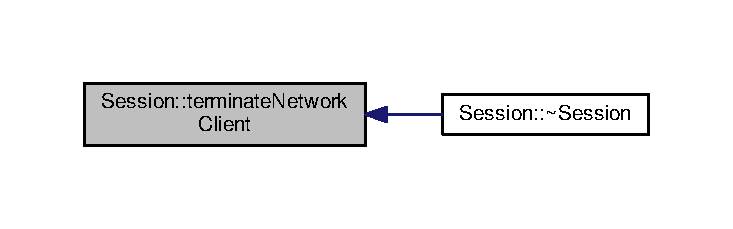
\includegraphics[width=350pt]{class_session_ad74cf272a2adfaa0a2abcaf31dde167d_icgraph}
\end{center}
\end{figure}


\hypertarget{class_session_ab3c9282517142617d9daf5ea08768083}{\index{Session@{Session}!terminate\-Network\-Server@{terminate\-Network\-Server}}
\index{terminate\-Network\-Server@{terminate\-Network\-Server}!Session@{Session}}
\subsubsection[{terminate\-Network\-Server}]{\setlength{\rightskip}{0pt plus 5cm}void Session\-::terminate\-Network\-Server (
\begin{DoxyParamCaption}
{}
\end{DoxyParamCaption}
)}}\label{class_session_ab3c9282517142617d9daf5ea08768083}

\begin{DoxyCode}
355 \{
356     \textcolor{keywordflow}{if} (!\hyperlink{class_session_a0f513f8d52d5026a3c449738da984c29}{myNetServer})
357         \textcolor{keywordflow}{return}; \textcolor{comment}{// already terminated}
358     \hyperlink{class_session_a0f513f8d52d5026a3c449738da984c29}{myNetServer}->SignalTerminationAll();
359     \textcolor{comment}{// Give the thread some time to terminate.}
360     \textcolor{keywordflow}{if} (\hyperlink{class_session_a0f513f8d52d5026a3c449738da984c29}{myNetServer}->JoinAll(\textcolor{keyword}{true}))
361         \hyperlink{class_session_a0f513f8d52d5026a3c449738da984c29}{myNetServer}.reset();
362     \textcolor{comment}{// If termination fails, leave a memory leak to prevent a crash.}
363 \}
\end{DoxyCode}


이 함수를 호출하는 함수들에 대한 그래프입니다.\-:\nopagebreak
\begin{figure}[H]
\begin{center}
\leavevmode
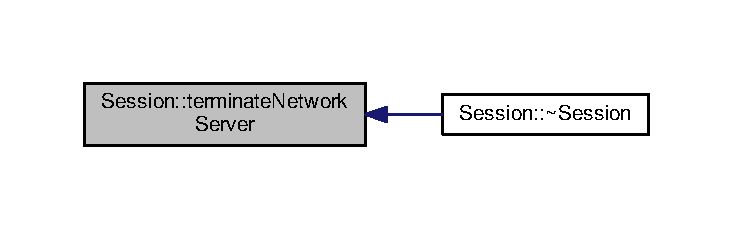
\includegraphics[width=350pt]{class_session_ab3c9282517142617d9daf5ea08768083_icgraph}
\end{center}
\end{figure}


\hypertarget{class_session_a346c8fa2d61d205f825c2af8a12d2071}{\index{Session@{Session}!vote\-Kick@{vote\-Kick}}
\index{vote\-Kick@{vote\-Kick}!Session@{Session}}
\subsubsection[{vote\-Kick}]{\setlength{\rightskip}{0pt plus 5cm}void Session\-::vote\-Kick (
\begin{DoxyParamCaption}
\item[{bool}]{do\-Kick}
\end{DoxyParamCaption}
)}}\label{class_session_a346c8fa2d61d205f825c2af8a12d2071}

\begin{DoxyCode}
522 \{
523     \textcolor{keywordflow}{if} (!\hyperlink{class_session_a767e3250d6a14be4c2b86d1e2dfa7b3c}{myNetClient})
524         \textcolor{keywordflow}{return}; \textcolor{comment}{// only act if client is running.}
525     \hyperlink{class_session_a767e3250d6a14be4c2b86d1e2dfa7b3c}{myNetClient}->SendVoteKick(doKick);
526 \}
\end{DoxyCode}


\subsection{멤버 데이타 문서화}
\hypertarget{class_session_a5c15d5f1be74a30fa167a0af5822113c}{\index{Session@{Session}!current\-Game@{current\-Game}}
\index{current\-Game@{current\-Game}!Session@{Session}}
\subsubsection[{current\-Game}]{\setlength{\rightskip}{0pt plus 5cm}boost\-::shared\-\_\-ptr$<$Game$>$ Session\-::current\-Game\hspace{0.3cm}{\ttfamily [private]}}}\label{class_session_a5c15d5f1be74a30fa167a0af5822113c}
\hypertarget{class_session_a89974964b38a285de9ec954b99b0ee3f}{\index{Session@{Session}!current\-Game\-Num@{current\-Game\-Num}}
\index{current\-Game\-Num@{current\-Game\-Num}!Session@{Session}}
\subsubsection[{current\-Game\-Num}]{\setlength{\rightskip}{0pt plus 5cm}int Session\-::current\-Game\-Num\hspace{0.3cm}{\ttfamily [private]}}}\label{class_session_a89974964b38a285de9ec954b99b0ee3f}
\hypertarget{class_session_a53231528d2b4c4babd97c7d1194a5f7e}{\index{Session@{Session}!my\-Avatar\-Manager@{my\-Avatar\-Manager}}
\index{my\-Avatar\-Manager@{my\-Avatar\-Manager}!Session@{Session}}
\subsubsection[{my\-Avatar\-Manager}]{\setlength{\rightskip}{0pt plus 5cm}boost\-::shared\-\_\-ptr$<$Avatar\-Manager$>$ Session\-::my\-Avatar\-Manager\hspace{0.3cm}{\ttfamily [private]}}}\label{class_session_a53231528d2b4c4babd97c7d1194a5f7e}
\hypertarget{class_session_a5bfbe43c623b688e7def57e02704033f}{\index{Session@{Session}!my\-Config@{my\-Config}}
\index{my\-Config@{my\-Config}!Session@{Session}}
\subsubsection[{my\-Config}]{\setlength{\rightskip}{0pt plus 5cm}Config\-File$\ast$ Session\-::my\-Config\hspace{0.3cm}{\ttfamily [private]}}}\label{class_session_a5bfbe43c623b688e7def57e02704033f}
\hypertarget{class_session_acf11b7b3982bc3e4c5bbf635d5e98496}{\index{Session@{Session}!my\-Game\-Type@{my\-Game\-Type}}
\index{my\-Game\-Type@{my\-Game\-Type}!Session@{Session}}
\subsubsection[{my\-Game\-Type}]{\setlength{\rightskip}{0pt plus 5cm}{\bf Game\-Type} Session\-::my\-Game\-Type\hspace{0.3cm}{\ttfamily [private]}}}\label{class_session_acf11b7b3982bc3e4c5bbf635d5e98496}
\hypertarget{class_session_a2725f4b56b109b2e7d75ed780d24fa6d}{\index{Session@{Session}!my\-Gui@{my\-Gui}}
\index{my\-Gui@{my\-Gui}!Session@{Session}}
\subsubsection[{my\-Gui}]{\setlength{\rightskip}{0pt plus 5cm}Gui\-Interface$\ast$ Session\-::my\-Gui\hspace{0.3cm}{\ttfamily [private]}}}\label{class_session_a2725f4b56b109b2e7d75ed780d24fa6d}
\hypertarget{class_session_a95063949539c8584d569d777284784ba}{\index{Session@{Session}!my\-Irc\-Nick@{my\-Irc\-Nick}}
\index{my\-Irc\-Nick@{my\-Irc\-Nick}!Session@{Session}}
\subsubsection[{my\-Irc\-Nick}]{\setlength{\rightskip}{0pt plus 5cm}std\-::string Session\-::my\-Irc\-Nick\hspace{0.3cm}{\ttfamily [private]}}}\label{class_session_a95063949539c8584d569d777284784ba}
\hypertarget{class_session_a1d2dd8533f3c551a5c18211f22d380f8}{\index{Session@{Session}!my\-Log@{my\-Log}}
\index{my\-Log@{my\-Log}!Session@{Session}}
\subsubsection[{my\-Log}]{\setlength{\rightskip}{0pt plus 5cm}Log$\ast$ Session\-::my\-Log\hspace{0.3cm}{\ttfamily [private]}}}\label{class_session_a1d2dd8533f3c551a5c18211f22d380f8}
\hypertarget{class_session_a767e3250d6a14be4c2b86d1e2dfa7b3c}{\index{Session@{Session}!my\-Net\-Client@{my\-Net\-Client}}
\index{my\-Net\-Client@{my\-Net\-Client}!Session@{Session}}
\subsubsection[{my\-Net\-Client}]{\setlength{\rightskip}{0pt plus 5cm}boost\-::shared\-\_\-ptr$<$Client\-Thread$>$ Session\-::my\-Net\-Client\hspace{0.3cm}{\ttfamily [private]}}}\label{class_session_a767e3250d6a14be4c2b86d1e2dfa7b3c}
\hypertarget{class_session_a0f513f8d52d5026a3c449738da984c29}{\index{Session@{Session}!my\-Net\-Server@{my\-Net\-Server}}
\index{my\-Net\-Server@{my\-Net\-Server}!Session@{Session}}
\subsubsection[{my\-Net\-Server}]{\setlength{\rightskip}{0pt plus 5cm}boost\-::shared\-\_\-ptr$<$Server\-Manager$>$ Session\-::my\-Net\-Server\hspace{0.3cm}{\ttfamily [private]}}}\label{class_session_a0f513f8d52d5026a3c449738da984c29}
\hypertarget{class_session_a1827a0341223eafa3859f249e73ebd38}{\index{Session@{Session}!my\-Qt\-Tools\-Interface@{my\-Qt\-Tools\-Interface}}
\index{my\-Qt\-Tools\-Interface@{my\-Qt\-Tools\-Interface}!Session@{Session}}
\subsubsection[{my\-Qt\-Tools\-Interface}]{\setlength{\rightskip}{0pt plus 5cm}Qt\-Tools\-Interface$\ast$ Session\-::my\-Qt\-Tools\-Interface\hspace{0.3cm}{\ttfamily [private]}}}\label{class_session_a1827a0341223eafa3859f249e73ebd38}


이 클래스에 대한 문서화 페이지는 다음의 파일들로부터 생성되었습니다.\-:\begin{DoxyCompactItemize}
\item 
\hyperlink{session_8h}{session.\-h}\item 
\hyperlink{session_8cpp}{session.\-cpp}\end{DoxyCompactItemize}

\hypertarget{struct_start_data}{\section{Start\-Data 구조체 참조}
\label{struct_start_data}\index{Start\-Data@{Start\-Data}}
}


{\ttfamily \#include $<$gamedata.\-h$>$}



Start\-Data에 대한 협력 다이어그램\-:\nopagebreak
\begin{figure}[H]
\begin{center}
\leavevmode
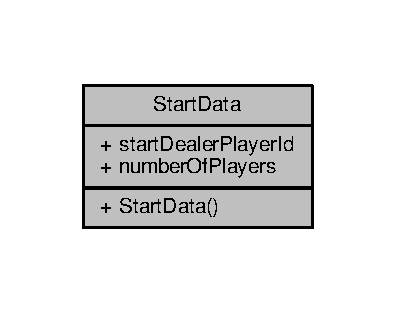
\includegraphics[width=190pt]{struct_start_data__coll__graph}
\end{center}
\end{figure}
\subsection*{Public 멤버 함수}
\begin{DoxyCompactItemize}
\item 
\hyperlink{struct_start_data_a5595be90248afdc5a1f9e3b0aee5ce92}{Start\-Data} ()
\end{DoxyCompactItemize}
\subsection*{Public 속성}
\begin{DoxyCompactItemize}
\item 
unsigned \hyperlink{struct_start_data_a3857fbb0e5191f2352fcee6c891c704f}{start\-Dealer\-Player\-Id}
\item 
int \hyperlink{struct_start_data_a962ea391fe81cc9d28ac7ec7ea511afc}{number\-Of\-Players}
\end{DoxyCompactItemize}


\subsection{생성자 \& 소멸자 문서화}
\hypertarget{struct_start_data_a5595be90248afdc5a1f9e3b0aee5ce92}{\index{Start\-Data@{Start\-Data}!Start\-Data@{Start\-Data}}
\index{Start\-Data@{Start\-Data}!StartData@{Start\-Data}}
\subsubsection[{Start\-Data}]{\setlength{\rightskip}{0pt plus 5cm}Start\-Data\-::\-Start\-Data (
\begin{DoxyParamCaption}
{}
\end{DoxyParamCaption}
)\hspace{0.3cm}{\ttfamily [inline]}}}\label{struct_start_data_a5595be90248afdc5a1f9e3b0aee5ce92}

\begin{DoxyCode}
111 : \hyperlink{struct_start_data_a3857fbb0e5191f2352fcee6c891c704f}{startDealerPlayerId}(0), \hyperlink{struct_start_data_a962ea391fe81cc9d28ac7ec7ea511afc}{numberOfPlayers}(0) \{\}
\end{DoxyCode}


\subsection{멤버 데이타 문서화}
\hypertarget{struct_start_data_a962ea391fe81cc9d28ac7ec7ea511afc}{\index{Start\-Data@{Start\-Data}!number\-Of\-Players@{number\-Of\-Players}}
\index{number\-Of\-Players@{number\-Of\-Players}!StartData@{Start\-Data}}
\subsubsection[{number\-Of\-Players}]{\setlength{\rightskip}{0pt plus 5cm}int Start\-Data\-::number\-Of\-Players}}\label{struct_start_data_a962ea391fe81cc9d28ac7ec7ea511afc}
\hypertarget{struct_start_data_a3857fbb0e5191f2352fcee6c891c704f}{\index{Start\-Data@{Start\-Data}!start\-Dealer\-Player\-Id@{start\-Dealer\-Player\-Id}}
\index{start\-Dealer\-Player\-Id@{start\-Dealer\-Player\-Id}!StartData@{Start\-Data}}
\subsubsection[{start\-Dealer\-Player\-Id}]{\setlength{\rightskip}{0pt plus 5cm}unsigned Start\-Data\-::start\-Dealer\-Player\-Id}}\label{struct_start_data_a3857fbb0e5191f2352fcee6c891c704f}


이 구조체에 대한 문서화 페이지는 다음의 파일로부터 생성되었습니다.\-:\begin{DoxyCompactItemize}
\item 
\hyperlink{gamedata_8h}{gamedata.\-h}\end{DoxyCompactItemize}

\hypertarget{struct_vote_kick_data}{\section{Vote\-Kick\-Data 구조체 참조}
\label{struct_vote_kick_data}\index{Vote\-Kick\-Data@{Vote\-Kick\-Data}}
}


{\ttfamily \#include $<$gamedata.\-h$>$}



Vote\-Kick\-Data에 대한 협력 다이어그램\-:\nopagebreak
\begin{figure}[H]
\begin{center}
\leavevmode
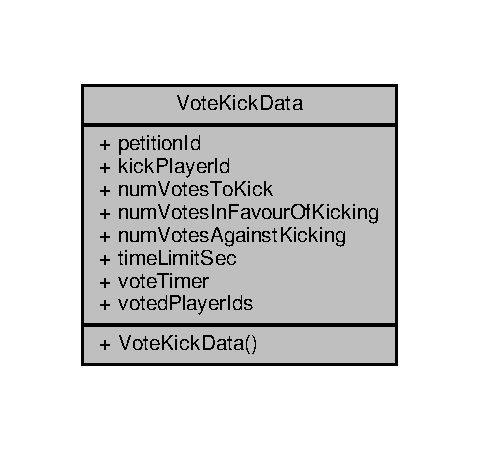
\includegraphics[width=230pt]{struct_vote_kick_data__coll__graph}
\end{center}
\end{figure}
\subsection*{Public 멤버 함수}
\begin{DoxyCompactItemize}
\item 
\hyperlink{struct_vote_kick_data_a4c0969c2c429557a27eaeff81f6ff58a}{Vote\-Kick\-Data} ()
\end{DoxyCompactItemize}
\subsection*{Public 속성}
\begin{DoxyCompactItemize}
\item 
unsigned \hyperlink{struct_vote_kick_data_a8deeb29aef91634e9082ca4f79780aa9}{petition\-Id}
\item 
unsigned \hyperlink{struct_vote_kick_data_a6086ee81bbafdd51a66dfcbc33e74ea2}{kick\-Player\-Id}
\item 
int \hyperlink{struct_vote_kick_data_aa0004f4d5672181658012cd3a92d4a8f}{num\-Votes\-To\-Kick}
\item 
int \hyperlink{struct_vote_kick_data_ab5832617a09a60929e6eff903f15d981}{num\-Votes\-In\-Favour\-Of\-Kicking}
\item 
int \hyperlink{struct_vote_kick_data_aec0801b812692d84c9abce891e8fefcd}{num\-Votes\-Against\-Kicking}
\item 
int \hyperlink{struct_vote_kick_data_a79e16bf0cf655c6de32eb21beecaf3bf}{time\-Limit\-Sec}
\item 
boost\-::timers\-::portable\-::microsec\-\_\-timer \hyperlink{struct_vote_kick_data_a0a4074bb3ceb4760b27403e1fd67c45d}{vote\-Timer}
\item 
\hyperlink{gamedata_8h_a02ee63ca030dfa9d119c9f2df584e383}{Player\-Id\-List} \hyperlink{struct_vote_kick_data_a68bb6a654755d931a50e4bc8ec27a67b}{voted\-Player\-Ids}
\end{DoxyCompactItemize}


\subsection{생성자 \& 소멸자 문서화}
\hypertarget{struct_vote_kick_data_a4c0969c2c429557a27eaeff81f6ff58a}{\index{Vote\-Kick\-Data@{Vote\-Kick\-Data}!Vote\-Kick\-Data@{Vote\-Kick\-Data}}
\index{Vote\-Kick\-Data@{Vote\-Kick\-Data}!VoteKickData@{Vote\-Kick\-Data}}
\subsubsection[{Vote\-Kick\-Data}]{\setlength{\rightskip}{0pt plus 5cm}Vote\-Kick\-Data\-::\-Vote\-Kick\-Data (
\begin{DoxyParamCaption}
{}
\end{DoxyParamCaption}
)\hspace{0.3cm}{\ttfamily [inline]}}}\label{struct_vote_kick_data_a4c0969c2c429557a27eaeff81f6ff58a}

\begin{DoxyCode}
118         : \hyperlink{struct_vote_kick_data_a8deeb29aef91634e9082ca4f79780aa9}{petitionId}(0), \hyperlink{struct_vote_kick_data_a6086ee81bbafdd51a66dfcbc33e74ea2}{kickPlayerId}(0), \hyperlink{struct_vote_kick_data_aa0004f4d5672181658012cd3a92d4a8f}{numVotesToKick}(0),
119           \hyperlink{struct_vote_kick_data_ab5832617a09a60929e6eff903f15d981}{numVotesInFavourOfKicking}(0), 
      \hyperlink{struct_vote_kick_data_aec0801b812692d84c9abce891e8fefcd}{numVotesAgainstKicking}(0), \hyperlink{struct_vote_kick_data_a79e16bf0cf655c6de32eb21beecaf3bf}{timeLimitSec}(0),
120           \hyperlink{struct_vote_kick_data_a0a4074bb3ceb4760b27403e1fd67c45d}{voteTimer}(boost::posix\_time::time\_duration(0, 0, 0), 
      boost::timers::portable::microsec\_timer::auto\_start) \{\}
\end{DoxyCode}


\subsection{멤버 데이타 문서화}
\hypertarget{struct_vote_kick_data_a6086ee81bbafdd51a66dfcbc33e74ea2}{\index{Vote\-Kick\-Data@{Vote\-Kick\-Data}!kick\-Player\-Id@{kick\-Player\-Id}}
\index{kick\-Player\-Id@{kick\-Player\-Id}!VoteKickData@{Vote\-Kick\-Data}}
\subsubsection[{kick\-Player\-Id}]{\setlength{\rightskip}{0pt plus 5cm}unsigned Vote\-Kick\-Data\-::kick\-Player\-Id}}\label{struct_vote_kick_data_a6086ee81bbafdd51a66dfcbc33e74ea2}
\hypertarget{struct_vote_kick_data_aec0801b812692d84c9abce891e8fefcd}{\index{Vote\-Kick\-Data@{Vote\-Kick\-Data}!num\-Votes\-Against\-Kicking@{num\-Votes\-Against\-Kicking}}
\index{num\-Votes\-Against\-Kicking@{num\-Votes\-Against\-Kicking}!VoteKickData@{Vote\-Kick\-Data}}
\subsubsection[{num\-Votes\-Against\-Kicking}]{\setlength{\rightskip}{0pt plus 5cm}int Vote\-Kick\-Data\-::num\-Votes\-Against\-Kicking}}\label{struct_vote_kick_data_aec0801b812692d84c9abce891e8fefcd}
\hypertarget{struct_vote_kick_data_ab5832617a09a60929e6eff903f15d981}{\index{Vote\-Kick\-Data@{Vote\-Kick\-Data}!num\-Votes\-In\-Favour\-Of\-Kicking@{num\-Votes\-In\-Favour\-Of\-Kicking}}
\index{num\-Votes\-In\-Favour\-Of\-Kicking@{num\-Votes\-In\-Favour\-Of\-Kicking}!VoteKickData@{Vote\-Kick\-Data}}
\subsubsection[{num\-Votes\-In\-Favour\-Of\-Kicking}]{\setlength{\rightskip}{0pt plus 5cm}int Vote\-Kick\-Data\-::num\-Votes\-In\-Favour\-Of\-Kicking}}\label{struct_vote_kick_data_ab5832617a09a60929e6eff903f15d981}
\hypertarget{struct_vote_kick_data_aa0004f4d5672181658012cd3a92d4a8f}{\index{Vote\-Kick\-Data@{Vote\-Kick\-Data}!num\-Votes\-To\-Kick@{num\-Votes\-To\-Kick}}
\index{num\-Votes\-To\-Kick@{num\-Votes\-To\-Kick}!VoteKickData@{Vote\-Kick\-Data}}
\subsubsection[{num\-Votes\-To\-Kick}]{\setlength{\rightskip}{0pt plus 5cm}int Vote\-Kick\-Data\-::num\-Votes\-To\-Kick}}\label{struct_vote_kick_data_aa0004f4d5672181658012cd3a92d4a8f}
\hypertarget{struct_vote_kick_data_a8deeb29aef91634e9082ca4f79780aa9}{\index{Vote\-Kick\-Data@{Vote\-Kick\-Data}!petition\-Id@{petition\-Id}}
\index{petition\-Id@{petition\-Id}!VoteKickData@{Vote\-Kick\-Data}}
\subsubsection[{petition\-Id}]{\setlength{\rightskip}{0pt plus 5cm}unsigned Vote\-Kick\-Data\-::petition\-Id}}\label{struct_vote_kick_data_a8deeb29aef91634e9082ca4f79780aa9}
\hypertarget{struct_vote_kick_data_a79e16bf0cf655c6de32eb21beecaf3bf}{\index{Vote\-Kick\-Data@{Vote\-Kick\-Data}!time\-Limit\-Sec@{time\-Limit\-Sec}}
\index{time\-Limit\-Sec@{time\-Limit\-Sec}!VoteKickData@{Vote\-Kick\-Data}}
\subsubsection[{time\-Limit\-Sec}]{\setlength{\rightskip}{0pt plus 5cm}int Vote\-Kick\-Data\-::time\-Limit\-Sec}}\label{struct_vote_kick_data_a79e16bf0cf655c6de32eb21beecaf3bf}
\hypertarget{struct_vote_kick_data_a68bb6a654755d931a50e4bc8ec27a67b}{\index{Vote\-Kick\-Data@{Vote\-Kick\-Data}!voted\-Player\-Ids@{voted\-Player\-Ids}}
\index{voted\-Player\-Ids@{voted\-Player\-Ids}!VoteKickData@{Vote\-Kick\-Data}}
\subsubsection[{voted\-Player\-Ids}]{\setlength{\rightskip}{0pt plus 5cm}{\bf Player\-Id\-List} Vote\-Kick\-Data\-::voted\-Player\-Ids}}\label{struct_vote_kick_data_a68bb6a654755d931a50e4bc8ec27a67b}
\hypertarget{struct_vote_kick_data_a0a4074bb3ceb4760b27403e1fd67c45d}{\index{Vote\-Kick\-Data@{Vote\-Kick\-Data}!vote\-Timer@{vote\-Timer}}
\index{vote\-Timer@{vote\-Timer}!VoteKickData@{Vote\-Kick\-Data}}
\subsubsection[{vote\-Timer}]{\setlength{\rightskip}{0pt plus 5cm}boost\-::timers\-::portable\-::microsec\-\_\-timer Vote\-Kick\-Data\-::vote\-Timer}}\label{struct_vote_kick_data_a0a4074bb3ceb4760b27403e1fd67c45d}


이 구조체에 대한 문서화 페이지는 다음의 파일로부터 생성되었습니다.\-:\begin{DoxyCompactItemize}
\item 
\hyperlink{gamedata_8h}{gamedata.\-h}\end{DoxyCompactItemize}

\chapter{파일 문서화}
\hypertarget{connectivity_8cpp}{\section{connectivity.\-cpp 파일 참조}
\label{connectivity_8cpp}\index{connectivity.\-cpp@{connectivity.\-cpp}}
}
{\ttfamily \#include $<$boost/asio.\-hpp$>$}\\*
{\ttfamily \#include $<$third\-\_\-party/protobuf/pokerth.\-pb.\-h$>$}\\*
{\ttfamily \#include $<$net/netpacket.\-h$>$}\\*
{\ttfamily \#include $<$boost/program\-\_\-options.\-hpp$>$}\\*
{\ttfamily \#include $<$boost/array.\-hpp$>$}\\*
{\ttfamily \#include $<$third\-\_\-party/boost/timers.\-hpp$>$}\\*
{\ttfamily \#include $<$gsasl.\-h$>$}\\*
{\ttfamily \#include $<$iostream$>$}\\*
connectivity.\-cpp에 대한 include 의존 그래프\nopagebreak
\begin{figure}[H]
\begin{center}
\leavevmode
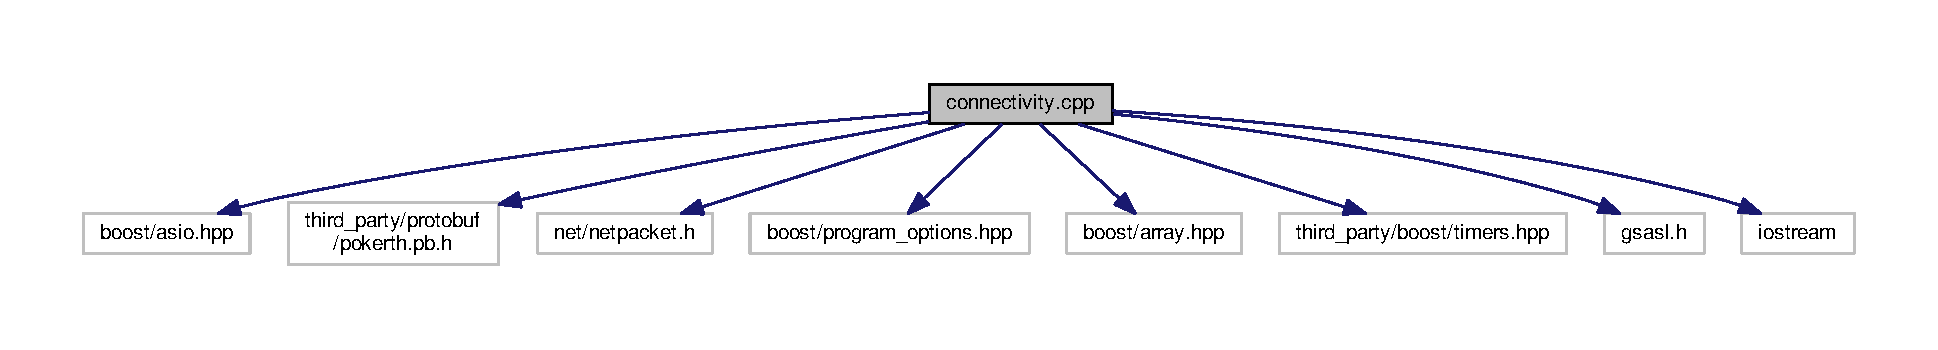
\includegraphics[width=350pt]{connectivity_8cpp__incl}
\end{center}
\end{figure}
\subsection*{매크로}
\begin{DoxyCompactItemize}
\item 
\#define \hyperlink{connectivity_8cpp_a6821bafc3c88dfb2e433a095df9940c6}{B\-U\-F\-\_\-\-S\-I\-Z\-E}~1024
\end{DoxyCompactItemize}
\subsection*{함수}
\begin{DoxyCompactItemize}
\item 
static int \hyperlink{connectivity_8cpp_a3648412ef7ef48b734fad6e3be1ff5c0}{net\-\_\-packet\-\_\-print\-\_\-to\-\_\-string} (const void $\ast$buffer, size\-\_\-t size, void $\ast$packet\-Str)
\item 
boost\-::shared\-\_\-ptr$<$ Net\-Packet $>$ \hyperlink{connectivity_8cpp_a3db166c2475ef569e071c9f128294a1e}{receive\-Message} (tcp\-::socket \&socket)
\item 
bool \hyperlink{connectivity_8cpp_afe10f9a10fbbf5b5a07cf0855ada9b53}{send\-Message} (tcp\-::socket \&socket, boost\-::shared\-\_\-ptr$<$ Net\-Packet $>$ packet)
\item 
int \hyperlink{connectivity_8cpp_a0ddf1224851353fc92bfbff6f499fa97}{main} (int argc, char $\ast$argv\mbox{[}$\,$\mbox{]})
\end{DoxyCompactItemize}
\subsection*{변수}
\begin{DoxyCompactItemize}
\item 
boost\-::array$<$ char, \hyperlink{load_8cpp_a6821bafc3c88dfb2e433a095df9940c6}{B\-U\-F\-\_\-\-S\-I\-Z\-E} $>$ \hyperlink{connectivity_8cpp_a28c52791e1c4323ccaf064585b2c0780}{rec\-Buf}
\item 
size\-\_\-t \hyperlink{connectivity_8cpp_a2f5de438cdc19635fc6c748abd642d98}{rec\-Buf\-Pos} = 0
\item 
boost\-::array$<$ char, \hyperlink{load_8cpp_a6821bafc3c88dfb2e433a095df9940c6}{B\-U\-F\-\_\-\-S\-I\-Z\-E} $>$ \hyperlink{connectivity_8cpp_a3ae560cc1fe6939622ae458627023bc2}{send\-Buf}
\end{DoxyCompactItemize}


\subsection{매크로 문서화}
\hypertarget{connectivity_8cpp_a6821bafc3c88dfb2e433a095df9940c6}{\index{connectivity.\-cpp@{connectivity.\-cpp}!B\-U\-F\-\_\-\-S\-I\-Z\-E@{B\-U\-F\-\_\-\-S\-I\-Z\-E}}
\index{B\-U\-F\-\_\-\-S\-I\-Z\-E@{B\-U\-F\-\_\-\-S\-I\-Z\-E}!connectivity.cpp@{connectivity.\-cpp}}
\subsubsection[{B\-U\-F\-\_\-\-S\-I\-Z\-E}]{\setlength{\rightskip}{0pt plus 5cm}\#define B\-U\-F\-\_\-\-S\-I\-Z\-E~1024}}\label{connectivity_8cpp_a6821bafc3c88dfb2e433a095df9940c6}


\subsection{함수 문서화}
\hypertarget{connectivity_8cpp_a0ddf1224851353fc92bfbff6f499fa97}{\index{connectivity.\-cpp@{connectivity.\-cpp}!main@{main}}
\index{main@{main}!connectivity.cpp@{connectivity.\-cpp}}
\subsubsection[{main}]{\setlength{\rightskip}{0pt plus 5cm}int main (
\begin{DoxyParamCaption}
\item[{int}]{argc, }
\item[{char $\ast$}]{argv\mbox{[}$\,$\mbox{]}}
\end{DoxyParamCaption}
)}}\label{connectivity_8cpp_a0ddf1224851353fc92bfbff6f499fa97}

\begin{DoxyCode}
127 \{
128     \textcolor{keywordflow}{try} \{
129         \textcolor{comment}{// Check command line options.}
130         po::options\_description desc(\textcolor{stringliteral}{"Allowed options"});
131         desc.add\_options()
132         (\textcolor{stringliteral}{"help,h"}, \textcolor{stringliteral}{"produce help message"})
133         (\textcolor{stringliteral}{"server,s"}, po::value<string>(), \textcolor{stringliteral}{"PokerTH server name"})
134         (\textcolor{stringliteral}{"port,P"}, po::value<string>(), \textcolor{stringliteral}{"PokerTH server port"})
135         (\textcolor{stringliteral}{"mode,m"}, po::value<int>(), \textcolor{stringliteral}{"set mode (0=connection test, 1=lag test)"})
136         (\textcolor{stringliteral}{"username,u"}, po::value<string>(), \textcolor{stringliteral}{"user name used for test"})
137         (\textcolor{stringliteral}{"password,p"}, po::value<string>(), \textcolor{stringliteral}{"password used for test"})
138         ;
139 
140         po::variables\_map vm;
141         po::store(po::parse\_command\_line(argc, argv, desc), vm);
142         po::notify(vm);
143 
144         \textcolor{keywordflow}{if} (vm.count(\textcolor{stringliteral}{"help"})) \{
145             cout << desc << endl;
146             \textcolor{keywordflow}{return} 1;
147         \}
148         \textcolor{keywordflow}{if} (!vm.count(\textcolor{stringliteral}{"server"}) || !vm.count(\textcolor{stringliteral}{"port"}) || !vm.count(\textcolor{stringliteral}{"mode"}) || !vm.count(\textcolor{stringliteral}{"username"})) \{
149             cout << \textcolor{stringliteral}{"Missing option!"} << endl << desc << endl;
150             \textcolor{keywordflow}{return} 1;
151         \}
152 
153         \textcolor{keywordtype}{string} server(vm[\textcolor{stringliteral}{"server"}].as<string>());
154         \textcolor{keywordtype}{string} port = vm[\textcolor{stringliteral}{"port"}].as<\textcolor{keywordtype}{string}>();
155         \textcolor{keywordtype}{int} mode = vm[\textcolor{stringliteral}{"mode"}].as<\textcolor{keywordtype}{int}>();
156         \textcolor{keywordtype}{string} username(vm[\textcolor{stringliteral}{"username"}].as<string>());
157         \textcolor{keywordtype}{string} password;
158         \textcolor{keywordflow}{if} (vm.count(\textcolor{stringliteral}{"password"})) \{
159             password = vm[\textcolor{stringliteral}{"password"}].as<\textcolor{keywordtype}{string}>();
160         \}
161         \textcolor{comment}{// Initialise gsasl.}
162         Gsasl *authContext;
163         Gsasl\_session *authSession;
164         \textcolor{keywordtype}{int} res = gsasl\_init(&authContext);
165         \textcolor{keywordflow}{if} (res != GSASL\_OK) \{
166             cout << \textcolor{stringliteral}{"gsasl init failed"} << endl;
167             \textcolor{keywordflow}{return} 1;
168         \}
169 
170         \textcolor{keywordflow}{if} (!gsasl\_client\_support\_p(authContext, \textcolor{stringliteral}{"SCRAM-SHA-1"})) \{
171             gsasl\_done(authContext);
172             cout << \textcolor{stringliteral}{"This version of gsasl does not support SCRAM-SHA-1"} << endl;
173             \textcolor{keywordflow}{return} 1;
174         \}
175 
176         \textcolor{comment}{// Connect to the PokerTH server.}
177         boost::timers::portable::microsec\_timer perfTimer;
178         boost::asio::io\_service io\_service;
179         tcp::resolver resolver(io\_service);
180         tcp::resolver::query query(server, port);
181         tcp::resolver::iterator endpoint\_iterator = resolver.resolve(query);
182         tcp::resolver::iterator end;
183         tcp::socket socket(io\_service);
184         boost::system::error\_code error = boost::asio::error::host\_not\_found;
185         \textcolor{keywordflow}{while} (error && endpoint\_iterator != end) \{
186             socket.close();
187             socket.connect(*endpoint\_iterator++, error);
188         \}
189         \textcolor{keywordflow}{if} (error) \{
190             cout << \textcolor{stringliteral}{"Connect failed"} << endl;
191             \textcolor{keywordflow}{return} 1;
192         \}
193         \textcolor{keywordflow}{if} (mode == 1) \{
194             cout << \textcolor{stringliteral}{"Connect.value "} << perfTimer.elapsed().total\_milliseconds() << endl;
195         \}
196         perfTimer.restart();
197 
198         \textcolor{comment}{// Receive server information}
199         boost::shared\_ptr<NetPacket> msg = \hyperlink{connectivity_8cpp_a3db166c2475ef569e071c9f128294a1e}{receiveMessage}(socket);
200         \textcolor{keywordflow}{if} (!msg || msg->GetMsg()->messagetype() != PokerTHMessage\_PokerTHMessageType\_Type\_AnnounceMessage)
       \{
201             cout << \textcolor{stringliteral}{"Announce failed"} << endl;
202             \textcolor{keywordflow}{return} 1;
203         \}
204 
205         \textcolor{comment}{// Send init}
206         msg.reset(\textcolor{keyword}{new} NetPacket);
207         msg->GetMsg()->set\_messagetype(PokerTHMessage\_PokerTHMessageType\_Type\_InitMessage);
208         InitMessage *netInit = msg->GetMsg()->mutable\_initmessage();
209         netInit->mutable\_requestedversion()->set\_majorversion(NET\_VERSION\_MAJOR);
210         netInit->mutable\_requestedversion()->set\_minorversion(NET\_VERSION\_MINOR);
211         netInit->set\_buildid(0);
212         \textcolor{keywordflow}{if} (password.empty()) \{
213             netInit->set\_login(InitMessage\_LoginType\_guestLogin);
214             netInit->set\_nickname(username);
215             \textcolor{keywordflow}{if} (!\hyperlink{connectivity_8cpp_afe10f9a10fbbf5b5a07cf0855ada9b53}{sendMessage}(socket, msg)) \{
216                 cout << \textcolor{stringliteral}{"Init guest failed"} << endl;
217                 \textcolor{keywordflow}{return} 1;
218             \}
219         \} \textcolor{keywordflow}{else} \{
220             \textcolor{keywordtype}{int} errorCode = gsasl\_client\_start(authContext, \textcolor{stringliteral}{"SCRAM-SHA-1"}, &authSession);
221             \textcolor{keywordflow}{if} (errorCode == GSASL\_OK) \{
222                 gsasl\_property\_set(authSession, GSASL\_AUTHID, username.c\_str());
223                 gsasl\_property\_set(authSession, GSASL\_PASSWORD, password.c\_str());
224 
225                 netInit->set\_login(InitMessage\_LoginType\_authenticatedLogin);
226 
227                 \textcolor{keywordtype}{char} *tmpOut;
228                 \textcolor{keywordtype}{size\_t} tmpOutSize;
229                 \textcolor{keywordtype}{string} nextGsaslMsg;
230                 errorCode = gsasl\_step(authSession, NULL, 0, &tmpOut, &tmpOutSize);
231                 \textcolor{keywordflow}{if} (errorCode == GSASL\_NEEDS\_MORE) \{
232                     nextGsaslMsg = string(tmpOut, tmpOutSize);
233                 \} \textcolor{keywordflow}{else} \{
234                     cout << \textcolor{stringliteral}{"gsasl step 1 failed"} << endl;
235                     \textcolor{keywordflow}{return} 1;
236                 \}
237                 gsasl\_free(tmpOut);
238 
239                 netInit->set\_clientuserdata(nextGsaslMsg);
240                 \textcolor{keywordflow}{if} (!\hyperlink{connectivity_8cpp_afe10f9a10fbbf5b5a07cf0855ada9b53}{sendMessage}(socket, msg)) \{
241                     cout << \textcolor{stringliteral}{"Init auth request failed"} << endl;
242                     \textcolor{keywordflow}{return} 1;
243                 \}
244 
245                 msg = \hyperlink{connectivity_8cpp_a3db166c2475ef569e071c9f128294a1e}{receiveMessage}(socket);
246                 \textcolor{keywordflow}{if} (!msg || msg->GetMsg()->messagetype() != 
      PokerTHMessage\_PokerTHMessageType\_Type\_AuthServerChallengeMessage) \{
247                     cout << \textcolor{stringliteral}{"Auth request failed"} << endl;
248                     \textcolor{keywordflow}{return} 1;
249                 \}
250 
251                 \textcolor{keyword}{const} AuthServerChallengeMessage &netAuth = msg->GetMsg()->authserverchallengemessage();
252                 \textcolor{keywordtype}{string} challengeStr(netAuth.serverchallenge());
253                 errorCode = gsasl\_step(authSession, challengeStr.c\_str(), challengeStr.size(), &tmpOut, &
      tmpOutSize);
254                 \textcolor{keywordflow}{if} (errorCode == GSASL\_NEEDS\_MORE) \{
255                     nextGsaslMsg = string(tmpOut, tmpOutSize);
256                 \} \textcolor{keywordflow}{else} \{
257                     cout << \textcolor{stringliteral}{"gsasl step 2 failed"} << endl;
258                     \textcolor{keywordflow}{return} 1;
259                 \}
260                 gsasl\_free(tmpOut);
261                 msg.reset(\textcolor{keyword}{new} NetPacket);
262                 msg->GetMsg()->set\_messagetype(
      PokerTHMessage\_PokerTHMessageType\_Type\_AuthClientResponseMessage);
263                 AuthClientResponseMessage *outAuth = msg->GetMsg()->mutable\_authclientresponsemessage();
264                 outAuth->set\_clientresponse(nextGsaslMsg);
265                 \textcolor{keywordflow}{if} (!\hyperlink{connectivity_8cpp_afe10f9a10fbbf5b5a07cf0855ada9b53}{sendMessage}(socket, msg)) \{
266                     cout << \textcolor{stringliteral}{"Init auth response failed"} << endl;
267                     \textcolor{keywordflow}{return} 1;
268                 \}
269                 msg = \hyperlink{connectivity_8cpp_a3db166c2475ef569e071c9f128294a1e}{receiveMessage}(socket);
270                 \textcolor{keywordflow}{if} (!msg || msg->GetMsg()->messagetype() != 
      PokerTHMessage\_PokerTHMessageType\_Type\_AuthServerVerificationMessage) \{
271                     cout << \textcolor{stringliteral}{"Auth response failed"} << endl;
272                     \textcolor{keywordflow}{return} 1;
273                 \}
274             \}
275         \}
276 
277         \textcolor{comment}{// Receive init ack}
278         msg = \hyperlink{connectivity_8cpp_a3db166c2475ef569e071c9f128294a1e}{receiveMessage}(socket);
279         \textcolor{keywordflow}{if} (!msg || msg->GetMsg()->messagetype() != PokerTHMessage\_PokerTHMessageType\_Type\_InitAckMessage) 
      \{
280             cout << \textcolor{stringliteral}{"Init ack failed"} << endl;
281             \textcolor{keywordflow}{return} 1;
282         \}
283 
284         \textcolor{keywordflow}{if} (mode == 1) \{
285             cout << \textcolor{stringliteral}{"Init.value "} << perfTimer.elapsed().total\_milliseconds() << endl;
286         \}
287         perfTimer.restart();
288 
289         \textcolor{comment}{// Send create game}
290         msg.reset(\textcolor{keyword}{new} NetPacket);
291         msg->GetMsg()->set\_messagetype(PokerTHMessage\_PokerTHMessageType\_Type\_JoinNewGameMessage);
292         JoinNewGameMessage *joinNew = msg->GetMsg()->mutable\_joinnewgamemessage();
293         joinNew->set\_autoleave(\textcolor{keyword}{false});
294         NetGameInfo *tmpGameInfo = joinNew->mutable\_gameinfo();
295         \textcolor{keywordtype}{string} tmpGameName(\textcolor{stringliteral}{"\_perftest\_do\_not\_join\_"} + username);
296         tmpGameInfo->set\_netgametype(NetGameInfo\_NetGameType\_normalGame);
297         tmpGameInfo->set\_maxnumplayers(10);
298         tmpGameInfo->set\_raiseintervalmode(NetGameInfo\_RaiseIntervalMode\_raiseOnHandNum);
299         tmpGameInfo->set\_raiseeveryhands(5);
300         tmpGameInfo->set\_endraisemode(NetGameInfo\_EndRaiseMode\_keepLastBlind);
301         tmpGameInfo->set\_proposedguispeed(5);
302         tmpGameInfo->set\_delaybetweenhands(6);
303         tmpGameInfo->set\_playeractiontimeout(10);
304         tmpGameInfo->set\_endraisesmallblindvalue(0);
305         tmpGameInfo->set\_firstsmallblind(50);
306         tmpGameInfo->set\_startmoney(2000);
307         tmpGameInfo->set\_gamename(tmpGameName);
308         \textcolor{keywordtype}{string} tmpGamePassword(\textcolor{stringliteral}{"blah123"});
309         joinNew->set\_password(tmpGamePassword);
310         \textcolor{keywordflow}{if} (!\hyperlink{connectivity_8cpp_afe10f9a10fbbf5b5a07cf0855ada9b53}{sendMessage}(socket, msg)) \{
311             cout << \textcolor{stringliteral}{"Create game failed"} << endl;
312             \textcolor{keywordflow}{return} 1;
313         \}
314         \textcolor{comment}{// Receive join game ack}
315         \textcolor{keywordflow}{do} \{
316             msg = \hyperlink{connectivity_8cpp_a3db166c2475ef569e071c9f128294a1e}{receiveMessage}(socket);
317             \textcolor{keywordflow}{if} (!msg) \{
318                 cout << \textcolor{stringliteral}{"Receive in lobby failed"} << endl;
319                 \textcolor{keywordflow}{return} 1;
320             \}
321             \textcolor{keywordflow}{if} (msg->GetMsg()->messagetype() == PokerTHMessage\_PokerTHMessageType\_Type\_ErrorMessage) \{
322                 cout << \textcolor{stringliteral}{"Received error"} << endl;
323                 \textcolor{keywordflow}{return} 1;
324             \} \textcolor{keywordflow}{else} \textcolor{keywordflow}{if} (msg->GetMsg()->messagetype() == 
      PokerTHMessage\_PokerTHMessageType\_Type\_JoinGameFailedMessage) \{
325                 cout << \textcolor{stringliteral}{"Join game ack failed"} << endl;
326                 \textcolor{keywordflow}{return} 1;
327             \}
328         \} \textcolor{keywordflow}{while} (msg->GetMsg()->messagetype() != PokerTHMessage\_PokerTHMessageType\_Type\_JoinGameAckMessage)
      ;
329 
330         \textcolor{keywordflow}{if} (mode == 1) \{
331             cout << \textcolor{stringliteral}{"CreateGame.value "} << perfTimer.elapsed().total\_milliseconds() << endl;
332         \} \textcolor{keywordflow}{else} \{
333             cout << \textcolor{stringliteral}{"Success"} << endl;
334         \}
335         perfTimer.restart();
336         gsasl\_done(authContext);
337     \} \textcolor{keywordflow}{catch} (...) \{
338         cout << \textcolor{stringliteral}{"Exception caught"} << endl;
339         \textcolor{keywordflow}{return} 1;
340     \}
341 
342     \textcolor{keywordflow}{return} 0;
343 \}\end{DoxyCode}


이 함수 내부에서 호출하는 함수들에 대한 그래프입니다.\-:\nopagebreak
\begin{figure}[H]
\begin{center}
\leavevmode
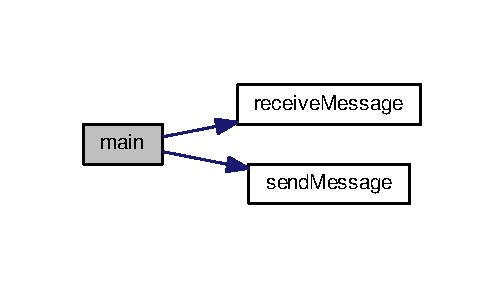
\includegraphics[width=242pt]{connectivity_8cpp_a0ddf1224851353fc92bfbff6f499fa97_cgraph}
\end{center}
\end{figure}


\hypertarget{connectivity_8cpp_a3648412ef7ef48b734fad6e3be1ff5c0}{\index{connectivity.\-cpp@{connectivity.\-cpp}!net\-\_\-packet\-\_\-print\-\_\-to\-\_\-string@{net\-\_\-packet\-\_\-print\-\_\-to\-\_\-string}}
\index{net\-\_\-packet\-\_\-print\-\_\-to\-\_\-string@{net\-\_\-packet\-\_\-print\-\_\-to\-\_\-string}!connectivity.cpp@{connectivity.\-cpp}}
\subsubsection[{net\-\_\-packet\-\_\-print\-\_\-to\-\_\-string}]{\setlength{\rightskip}{0pt plus 5cm}static int net\-\_\-packet\-\_\-print\-\_\-to\-\_\-string (
\begin{DoxyParamCaption}
\item[{const void $\ast$}]{buffer, }
\item[{size\-\_\-t}]{size, }
\item[{void $\ast$}]{packet\-Str}
\end{DoxyParamCaption}
)\hspace{0.3cm}{\ttfamily [static]}}}\label{connectivity_8cpp_a3648412ef7ef48b734fad6e3be1ff5c0}

\begin{DoxyCode}
56 \{
57     \textcolor{keywordtype}{string} *tmpString = (\textcolor{keywordtype}{string} *)packetStr;
58     *tmpString += string((\textcolor{keyword}{const} \textcolor{keywordtype}{char} *)buffer, size);
59     \textcolor{keywordflow}{return} 0;
60 \}
\end{DoxyCode}
\hypertarget{connectivity_8cpp_a3db166c2475ef569e071c9f128294a1e}{\index{connectivity.\-cpp@{connectivity.\-cpp}!receive\-Message@{receive\-Message}}
\index{receive\-Message@{receive\-Message}!connectivity.cpp@{connectivity.\-cpp}}
\subsubsection[{receive\-Message}]{\setlength{\rightskip}{0pt plus 5cm}boost\-::shared\-\_\-ptr$<$Net\-Packet$>$ receive\-Message (
\begin{DoxyParamCaption}
\item[{tcp\-::socket \&}]{socket}
\end{DoxyParamCaption}
)}}\label{connectivity_8cpp_a3db166c2475ef569e071c9f128294a1e}

\begin{DoxyCode}
64 \{
65     boost::shared\_ptr<NetPacket> tmpPacket;
66 
67     \textcolor{keywordflow}{do} \{
68         \textcolor{comment}{// This is necessary, because we use TCP.}
69         \textcolor{comment}{// Packets may be received in multiple chunks or}
70         \textcolor{comment}{// several packets may be received at once.}
71         \textcolor{keywordflow}{if} (\hyperlink{connectivity_8cpp_a2f5de438cdc19635fc6c748abd642d98}{recBufPos} >= NET\_HEADER\_SIZE) \{
72             \textcolor{comment}{// Read the size of the packet (first 4 bytes in network byte order).}
73             uint32\_t nativeVal;
74             memcpy(&nativeVal, \hyperlink{connectivity_8cpp_a28c52791e1c4323ccaf064585b2c0780}{recBuf}.c\_array(), \textcolor{keyword}{sizeof}(uint32\_t));
75             \textcolor{keywordtype}{size\_t} packetSize = ntohl(nativeVal);
76             \textcolor{keywordflow}{if} (packetSize > MAX\_PACKET\_SIZE) \{
77                 \hyperlink{connectivity_8cpp_a2f5de438cdc19635fc6c748abd642d98}{recBufPos} = 0;
78                 cout << \textcolor{stringliteral}{"Packet too large"} << endl;
79                 \textcolor{keywordflow}{return} boost::shared\_ptr<NetPacket>();
80             \} \textcolor{keywordflow}{else} \textcolor{keywordflow}{if} (\hyperlink{connectivity_8cpp_a2f5de438cdc19635fc6c748abd642d98}{recBufPos} >= packetSize + NET\_HEADER\_SIZE) \{
81                 \textcolor{keywordflow}{try} \{
82                     tmpPacket = NetPacket::Create(&\hyperlink{connectivity_8cpp_a28c52791e1c4323ccaf064585b2c0780}{recBuf}.c\_array()[NET\_HEADER\_SIZE], packetSize);
83                     \textcolor{keywordflow}{if} (tmpPacket) \{
84                         \hyperlink{connectivity_8cpp_a2f5de438cdc19635fc6c748abd642d98}{recBufPos} -= (packetSize + NET\_HEADER\_SIZE);
85                         \textcolor{keywordflow}{if} (\hyperlink{connectivity_8cpp_a2f5de438cdc19635fc6c748abd642d98}{recBufPos}) \{
86                             memmove(\hyperlink{connectivity_8cpp_a28c52791e1c4323ccaf064585b2c0780}{recBuf}.c\_array(), \hyperlink{connectivity_8cpp_a28c52791e1c4323ccaf064585b2c0780}{recBuf}.c\_array() + packetSize + 
      NET\_HEADER\_SIZE, \hyperlink{connectivity_8cpp_a2f5de438cdc19635fc6c748abd642d98}{recBufPos});
87                         \}
88                     \}
89                 \} \textcolor{keywordflow}{catch} (\textcolor{keyword}{const} exception &) \{
90                     \textcolor{comment}{// Reset buffer on error.}
91                     \hyperlink{connectivity_8cpp_a2f5de438cdc19635fc6c748abd642d98}{recBufPos} = 0;
92                     cout << \textcolor{stringliteral}{"Packet creation failed"} << endl;
93                     \textcolor{keywordflow}{return} boost::shared\_ptr<NetPacket>();
94                 \}
95             \}
96         \}
97 
98         \textcolor{keywordflow}{if} (!tmpPacket) \{
99             \hyperlink{connectivity_8cpp_a2f5de438cdc19635fc6c748abd642d98}{recBufPos} += socket.receive(boost::asio::buffer(\hyperlink{connectivity_8cpp_a28c52791e1c4323ccaf064585b2c0780}{recBuf}.c\_array() + 
      \hyperlink{connectivity_8cpp_a2f5de438cdc19635fc6c748abd642d98}{recBufPos}, \hyperlink{connectivity_8cpp_a6821bafc3c88dfb2e433a095df9940c6}{BUF\_SIZE} - \hyperlink{connectivity_8cpp_a2f5de438cdc19635fc6c748abd642d98}{recBufPos}));
100             \textcolor{keywordflow}{if} (\hyperlink{connectivity_8cpp_a2f5de438cdc19635fc6c748abd642d98}{recBufPos} == 0) \{
101                 cout << \textcolor{stringliteral}{"Receive failed"} << endl;
102                 \textcolor{keywordflow}{return} boost::shared\_ptr<NetPacket>();
103             \}
104         \}
105     \} \textcolor{keywordflow}{while} (!tmpPacket);
106 
107     \textcolor{keywordflow}{return} tmpPacket;
108 \}
\end{DoxyCode}


이 함수를 호출하는 함수들에 대한 그래프입니다.\-:\nopagebreak
\begin{figure}[H]
\begin{center}
\leavevmode
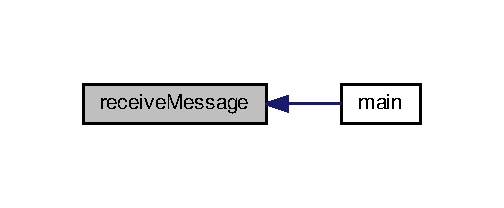
\includegraphics[width=242pt]{connectivity_8cpp_a3db166c2475ef569e071c9f128294a1e_icgraph}
\end{center}
\end{figure}


\hypertarget{connectivity_8cpp_afe10f9a10fbbf5b5a07cf0855ada9b53}{\index{connectivity.\-cpp@{connectivity.\-cpp}!send\-Message@{send\-Message}}
\index{send\-Message@{send\-Message}!connectivity.cpp@{connectivity.\-cpp}}
\subsubsection[{send\-Message}]{\setlength{\rightskip}{0pt plus 5cm}bool send\-Message (
\begin{DoxyParamCaption}
\item[{tcp\-::socket \&}]{socket, }
\item[{boost\-::shared\-\_\-ptr$<$ Net\-Packet $>$}]{packet}
\end{DoxyParamCaption}
)}}\label{connectivity_8cpp_afe10f9a10fbbf5b5a07cf0855ada9b53}

\begin{DoxyCode}
112 \{
113     \textcolor{keywordtype}{bool} retVal = \textcolor{keyword}{false};
114     \textcolor{keywordflow}{if} (packet) \{
115         uint32\_t packetSize = packet->GetMsg()->ByteSize();
116         google::protobuf::uint8 *buf = \textcolor{keyword}{new} google::protobuf::uint8[packetSize + NET\_HEADER\_SIZE];
117         *((uint32\_t *)buf) = htonl(packetSize);
118         packet->GetMsg()->SerializeWithCachedSizesToArray(&buf[NET\_HEADER\_SIZE]);
119         retVal = socket.send(boost::asio::buffer(buf, packetSize + NET\_HEADER\_SIZE)) != 0;
120         \textcolor{keyword}{delete}[] buf;
121     \}
122     \textcolor{keywordflow}{return} retVal;
123 \}
\end{DoxyCode}


이 함수를 호출하는 함수들에 대한 그래프입니다.\-:\nopagebreak
\begin{figure}[H]
\begin{center}
\leavevmode
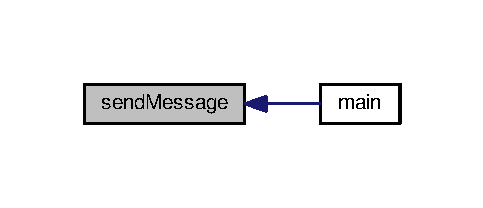
\includegraphics[width=232pt]{connectivity_8cpp_afe10f9a10fbbf5b5a07cf0855ada9b53_icgraph}
\end{center}
\end{figure}




\subsection{변수 문서화}
\hypertarget{connectivity_8cpp_a28c52791e1c4323ccaf064585b2c0780}{\index{connectivity.\-cpp@{connectivity.\-cpp}!rec\-Buf@{rec\-Buf}}
\index{rec\-Buf@{rec\-Buf}!connectivity.cpp@{connectivity.\-cpp}}
\subsubsection[{rec\-Buf}]{\setlength{\rightskip}{0pt plus 5cm}boost\-::array$<$char, {\bf B\-U\-F\-\_\-\-S\-I\-Z\-E}$>$ rec\-Buf}}\label{connectivity_8cpp_a28c52791e1c4323ccaf064585b2c0780}
\hypertarget{connectivity_8cpp_a2f5de438cdc19635fc6c748abd642d98}{\index{connectivity.\-cpp@{connectivity.\-cpp}!rec\-Buf\-Pos@{rec\-Buf\-Pos}}
\index{rec\-Buf\-Pos@{rec\-Buf\-Pos}!connectivity.cpp@{connectivity.\-cpp}}
\subsubsection[{rec\-Buf\-Pos}]{\setlength{\rightskip}{0pt plus 5cm}size\-\_\-t rec\-Buf\-Pos = 0}}\label{connectivity_8cpp_a2f5de438cdc19635fc6c748abd642d98}
\hypertarget{connectivity_8cpp_a3ae560cc1fe6939622ae458627023bc2}{\index{connectivity.\-cpp@{connectivity.\-cpp}!send\-Buf@{send\-Buf}}
\index{send\-Buf@{send\-Buf}!connectivity.cpp@{connectivity.\-cpp}}
\subsubsection[{send\-Buf}]{\setlength{\rightskip}{0pt plus 5cm}boost\-::array$<$char, {\bf B\-U\-F\-\_\-\-S\-I\-Z\-E}$>$ send\-Buf}}\label{connectivity_8cpp_a3ae560cc1fe6939622ae458627023bc2}

\hypertarget{game__defs_8h}{\section{game\-\_\-defs.\-h 파일 참조}
\label{game__defs_8h}\index{game\-\_\-defs.\-h@{game\-\_\-defs.\-h}}
}
이 그래프는 이 파일을 직/간접적으로 include 하는 파일들을 보여줍니다.\-:\nopagebreak
\begin{figure}[H]
\begin{center}
\leavevmode
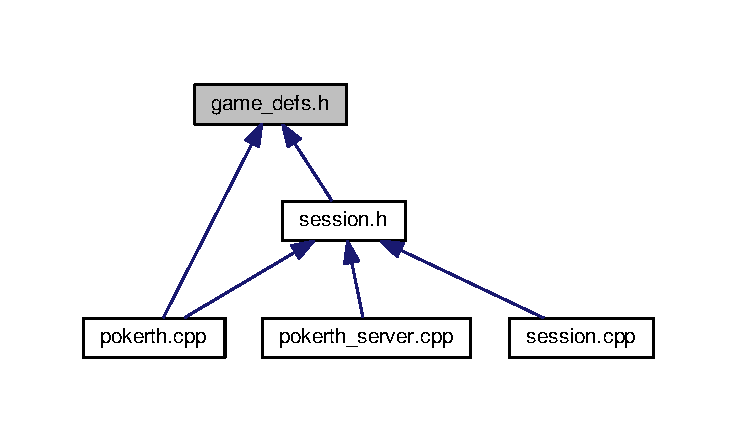
\includegraphics[width=350pt]{game__defs_8h__dep__incl}
\end{center}
\end{figure}
\subsection*{매크로}
\begin{DoxyCompactItemize}
\item 
\#define \hyperlink{game__defs_8h_a94504e403ec9ee86b059ee128c97352a}{M\-I\-N\-\_\-\-N\-U\-M\-B\-E\-R\-\_\-\-O\-F\-\_\-\-P\-L\-A\-Y\-E\-R\-S}~2
\item 
\#define \hyperlink{game__defs_8h_aae818a602d6311f97332e4f240f28135}{M\-A\-X\-\_\-\-N\-U\-M\-B\-E\-R\-\_\-\-O\-F\-\_\-\-P\-L\-A\-Y\-E\-R\-S}~10
\item 
\#define \hyperlink{game__defs_8h_ae848fe704b58cd40ef10fcc7e60d7747}{M\-I\-N\-\_\-\-G\-U\-I\-\_\-\-S\-P\-E\-E\-D}~1
\item 
\#define \hyperlink{game__defs_8h_ad558d6bbad70d9ab46227b6af70c6070}{M\-A\-X\-\_\-\-G\-U\-I\-\_\-\-S\-P\-E\-E\-D}~11
\item 
\#define \hyperlink{game__defs_8h_ab01498292cf5e8b38ecd3198ee194f31}{P\-O\-K\-E\-R\-T\-H\-\_\-\-V\-E\-R\-S\-I\-O\-N\-\_\-\-M\-A\-J\-O\-R}~1
\item 
\#define \hyperlink{game__defs_8h_a6334f1f1c54ffff22a17396f4afafe3b}{P\-O\-K\-E\-R\-T\-H\-\_\-\-V\-E\-R\-S\-I\-O\-N\-\_\-\-M\-I\-N\-O\-R}~11
\item 
\#define \hyperlink{game__defs_8h_a60b248c83b584df7c7f5ed9d45a281ba}{P\-O\-K\-E\-R\-T\-H\-\_\-\-V\-E\-R\-S\-I\-O\-N}~((\hyperlink{game__defs_8h_ab01498292cf5e8b38ecd3198ee194f31}{P\-O\-K\-E\-R\-T\-H\-\_\-\-V\-E\-R\-S\-I\-O\-N\-\_\-\-M\-A\-J\-O\-R} $<$$<$ 8) $\vert$ \hyperlink{game__defs_8h_a6334f1f1c54ffff22a17396f4afafe3b}{P\-O\-K\-E\-R\-T\-H\-\_\-\-V\-E\-R\-S\-I\-O\-N\-\_\-\-M\-I\-N\-O\-R})
\item 
\#define \hyperlink{game__defs_8h_a05875809d50ad1c742b994095176cc2c}{P\-O\-K\-E\-R\-T\-H\-\_\-\-B\-E\-T\-A\-\_\-\-R\-E\-V\-I\-S\-I\-O\-N}~0
\item 
\#define \hyperlink{game__defs_8h_ac16e1f5cf0ee8fbb4b1a0cd790e5f262}{P\-O\-K\-E\-R\-T\-H\-\_\-\-B\-E\-T\-A\-\_\-\-R\-E\-L\-E\-A\-S\-E\-\_\-\-S\-T\-R\-I\-N\-G}~\char`\"{}1.\-1.\-1\char`\"{}
\item 
\#define \hyperlink{game__defs_8h_a9c1c9a35e70f4452a8ad281fc937feaf}{S\-Q\-L\-I\-T\-E\-\_\-\-L\-O\-G\-\_\-\-V\-E\-R\-S\-I\-O\-N}~1
\item 
\#define \hyperlink{game__defs_8h_a2d4014e4ef9b0b5918d7f97b1171fd26}{R\-A\-N\-K\-I\-N\-G\-\_\-\-G\-A\-M\-E\-\_\-\-S\-T\-A\-R\-T\-\_\-\-C\-A\-S\-H}~10000
\item 
\#define \hyperlink{game__defs_8h_a5fc82b1b8ec959bf3bdc2412d225e41e}{R\-A\-N\-K\-I\-N\-G\-\_\-\-G\-A\-M\-E\-\_\-\-N\-U\-M\-B\-E\-R\-\_\-\-O\-F\-\_\-\-P\-L\-A\-Y\-E\-R\-S}~10
\item 
\#define \hyperlink{game__defs_8h_af1b3a95294d41b970d1e29f0abaf47e8}{R\-A\-N\-K\-I\-N\-G\-\_\-\-G\-A\-M\-E\-\_\-\-S\-T\-A\-R\-T\-\_\-\-S\-B\-L\-I\-N\-D}~50
\item 
\#define \hyperlink{game__defs_8h_af7fb2bdbe740b31998d788bdc6a48417}{R\-A\-N\-K\-I\-N\-G\-\_\-\-G\-A\-M\-E\-\_\-\-R\-A\-I\-S\-E\-\_\-\-E\-V\-E\-R\-Y\-\_\-\-H\-A\-N\-D}~11
\item 
\#define \hyperlink{game__defs_8h_a834e2654b05e24d90455b927975bf6dc}{L\-O\-G\-\_\-\-U\-P\-L\-O\-A\-D\-\_\-\-I\-D\-\_\-\-S\-I\-Z\-E}~40
\item 
\#define \hyperlink{game__defs_8h_a92fdd847e8934852f6240cbff7875c61}{L\-O\-G\-\_\-\-U\-P\-L\-O\-A\-D\-\_\-\-O\-K\-\_\-\-S\-T\-R}~\char`\"{}O\-K\char`\"{}
\item 
\#define \hyperlink{game__defs_8h_a1cc72893d2fbf44f18ee1da78124d490}{L\-O\-G\-\_\-\-U\-P\-L\-O\-A\-D\-\_\-\-E\-R\-R\-O\-R\-\_\-\-S\-T\-R}~\char`\"{}E\-R\-R\-O\-R\char`\"{}
\end{DoxyCompactItemize}
\subsection*{열거형 타입}
\begin{DoxyCompactItemize}
\item 
enum \hyperlink{game__defs_8h_a0c3cbd252a209f92f14db7a3d59a3956}{Server\-Mode} \{ \hyperlink{game__defs_8h_a0c3cbd252a209f92f14db7a3d59a3956a3f545f4f97970f80049cbbcafb0a565f}{S\-E\-R\-V\-E\-R\-\_\-\-M\-O\-D\-E\-\_\-\-L\-A\-N}, 
\hyperlink{game__defs_8h_a0c3cbd252a209f92f14db7a3d59a3956a7dffad0c975963f9853e2aba9bc4b156}{S\-E\-R\-V\-E\-R\-\_\-\-M\-O\-D\-E\-\_\-\-I\-N\-T\-E\-R\-N\-E\-T\-\_\-\-N\-O\-A\-U\-T\-H}, 
\hyperlink{game__defs_8h_a0c3cbd252a209f92f14db7a3d59a3956ad30e94a28f96a66c0d063ecd5ec237bb}{S\-E\-R\-V\-E\-R\-\_\-\-M\-O\-D\-E\-\_\-\-I\-N\-T\-E\-R\-N\-E\-T\-\_\-\-A\-U\-T\-H}, 
\hyperlink{game__defs_8h_a0c3cbd252a209f92f14db7a3d59a3956a2da97b4ed0833f737a1b67567b8b7f76}{S\-E\-R\-V\-E\-R\-\_\-\-M\-O\-D\-E\-\_\-\-L\-A\-N\-\_\-\-L\-O\-C\-A\-L}
 \}
\item 
enum \hyperlink{game__defs_8h_a16586aece3f2351978656f88132b23fc}{Server\-Transport\-Protocol} \{ \\*
\hyperlink{game__defs_8h_a16586aece3f2351978656f88132b23fcadd18d6cbb60ab77047bbb55a93cd82b8}{T\-R\-A\-N\-S\-P\-O\-R\-T\-\_\-\-P\-R\-O\-T\-O\-C\-O\-L\-\_\-\-T\-C\-P} = 1, 
\hyperlink{game__defs_8h_a16586aece3f2351978656f88132b23fca2f9ad9f5989b295874a0072e784fc833}{T\-R\-A\-N\-S\-P\-O\-R\-T\-\_\-\-P\-R\-O\-T\-O\-C\-O\-L\-\_\-\-S\-C\-T\-P} = 2, 
\hyperlink{game__defs_8h_a16586aece3f2351978656f88132b23fcac05734160dd9a0a8a6077b8ac331a204}{T\-R\-A\-N\-S\-P\-O\-R\-T\-\_\-\-P\-R\-O\-T\-O\-C\-O\-L\-\_\-\-T\-C\-P\-\_\-\-S\-C\-T\-P} = 3, 
\hyperlink{game__defs_8h_a16586aece3f2351978656f88132b23fca6c97945151581eabf3e61a835f68f53d}{T\-R\-A\-N\-S\-P\-O\-R\-T\-\_\-\-P\-R\-O\-T\-O\-C\-O\-L\-\_\-\-W\-E\-B\-S\-O\-C\-K\-E\-T} = 4, 
\\*
\hyperlink{game__defs_8h_a16586aece3f2351978656f88132b23fca3230f525e888a68621de1a9d21b78997}{T\-R\-A\-N\-S\-P\-O\-R\-T\-\_\-\-P\-R\-O\-T\-O\-C\-O\-L\-\_\-\-T\-C\-P\-\_\-\-W\-E\-B\-S\-O\-C\-K\-E\-T} = 5, 
\hyperlink{game__defs_8h_a16586aece3f2351978656f88132b23fca76fa354fe7f1d1784601f1929c715d4c}{T\-R\-A\-N\-S\-P\-O\-R\-T\-\_\-\-P\-R\-O\-T\-O\-C\-O\-L\-\_\-\-T\-C\-P\-\_\-\-S\-C\-T\-P\-\_\-\-W\-E\-B\-S\-O\-C\-K\-E\-T} = 7
 \}
\item 
enum \hyperlink{game__defs_8h_a7899b65f1ea0f655e4bbf8d2a5714285}{Game\-State} \{ \\*
\hyperlink{game__defs_8h_a7899b65f1ea0f655e4bbf8d2a5714285a94ed0f2402dd6cd903eeee97c2e3a922}{G\-A\-M\-E\-\_\-\-S\-T\-A\-T\-E\-\_\-\-P\-R\-E\-F\-L\-O\-P} = 0, 
\hyperlink{game__defs_8h_a7899b65f1ea0f655e4bbf8d2a5714285a8f3c19d7d097363f6d501224a97b1ee7}{G\-A\-M\-E\-\_\-\-S\-T\-A\-T\-E\-\_\-\-F\-L\-O\-P}, 
\hyperlink{game__defs_8h_a7899b65f1ea0f655e4bbf8d2a5714285a2bb918721414681b7a3a8e42bcea419c}{G\-A\-M\-E\-\_\-\-S\-T\-A\-T\-E\-\_\-\-T\-U\-R\-N}, 
\hyperlink{game__defs_8h_a7899b65f1ea0f655e4bbf8d2a5714285a58da5207e0c04f117e7347b953eaa777}{G\-A\-M\-E\-\_\-\-S\-T\-A\-T\-E\-\_\-\-R\-I\-V\-E\-R}, 
\\*
\hyperlink{game__defs_8h_a7899b65f1ea0f655e4bbf8d2a5714285ae33f9ffa4aa78ecefd293b4502fb4fd1}{G\-A\-M\-E\-\_\-\-S\-T\-A\-T\-E\-\_\-\-P\-O\-S\-T\-\_\-\-R\-I\-V\-E\-R}, 
\hyperlink{game__defs_8h_a7899b65f1ea0f655e4bbf8d2a5714285a8e7e655f181a88672dde7417192a851a}{G\-A\-M\-E\-\_\-\-S\-T\-A\-T\-E\-\_\-\-P\-R\-E\-F\-L\-O\-P\-\_\-\-S\-M\-A\-L\-L\-\_\-\-B\-L\-I\-N\-D} = 0x\-F0, 
\hyperlink{game__defs_8h_a7899b65f1ea0f655e4bbf8d2a5714285ac162b15215b6b8e32724cc5f75af578c}{G\-A\-M\-E\-\_\-\-S\-T\-A\-T\-E\-\_\-\-P\-R\-E\-F\-L\-O\-P\-\_\-\-B\-I\-G\-\_\-\-B\-L\-I\-N\-D} = 0x\-F1
 \}
\item 
enum \hyperlink{game__defs_8h_aea132397c26cad8f8637a9422260deca}{Player\-Action} \{ \\*
\hyperlink{game__defs_8h_aea132397c26cad8f8637a9422260decaa53642bc4dae0658ebb57c1fa0e6e08d6}{P\-L\-A\-Y\-E\-R\-\_\-\-A\-C\-T\-I\-O\-N\-\_\-\-N\-O\-N\-E} = 0, 
\hyperlink{game__defs_8h_aea132397c26cad8f8637a9422260decaae74248d5f8a69a6276d3058722c7317f}{P\-L\-A\-Y\-E\-R\-\_\-\-A\-C\-T\-I\-O\-N\-\_\-\-F\-O\-L\-D}, 
\hyperlink{game__defs_8h_aea132397c26cad8f8637a9422260decaaf6180f72aa239c5290fd09a8500ac6b0}{P\-L\-A\-Y\-E\-R\-\_\-\-A\-C\-T\-I\-O\-N\-\_\-\-C\-H\-E\-C\-K}, 
\hyperlink{game__defs_8h_aea132397c26cad8f8637a9422260decaa4ea1a7e65b5f8e553dcbe3eafe385657}{P\-L\-A\-Y\-E\-R\-\_\-\-A\-C\-T\-I\-O\-N\-\_\-\-C\-A\-L\-L}, 
\\*
\hyperlink{game__defs_8h_aea132397c26cad8f8637a9422260decaab2725fe3290652556263fc6df822d544}{P\-L\-A\-Y\-E\-R\-\_\-\-A\-C\-T\-I\-O\-N\-\_\-\-B\-E\-T}, 
\hyperlink{game__defs_8h_aea132397c26cad8f8637a9422260decaa922b57a9457c2e9fa0bdd4d2540ef5bf}{P\-L\-A\-Y\-E\-R\-\_\-\-A\-C\-T\-I\-O\-N\-\_\-\-R\-A\-I\-S\-E}, 
\hyperlink{game__defs_8h_aea132397c26cad8f8637a9422260decaa6c83d49d1f664533a04b98cff1215a0d}{P\-L\-A\-Y\-E\-R\-\_\-\-A\-C\-T\-I\-O\-N\-\_\-\-A\-L\-L\-I\-N}
 \}
\item 
enum \hyperlink{game__defs_8h_a7d35cfb14557a5e8a80d236e992e68a3}{Player\-Action\-Code} \{ \hyperlink{game__defs_8h_a7d35cfb14557a5e8a80d236e992e68a3aa9e0e7e62b916d5d7513c3569025a96d}{A\-C\-T\-I\-O\-N\-\_\-\-C\-O\-D\-E\-\_\-\-V\-A\-L\-I\-D} = 0, 
\hyperlink{game__defs_8h_a7d35cfb14557a5e8a80d236e992e68a3ab12098a083db1c3664caf73095e3458d}{A\-C\-T\-I\-O\-N\-\_\-\-C\-O\-D\-E\-\_\-\-I\-N\-V\-A\-L\-I\-D\-\_\-\-S\-T\-A\-T\-E}, 
\hyperlink{game__defs_8h_a7d35cfb14557a5e8a80d236e992e68a3a8ede6eefeca26e8ed80f98dd607c4a02}{A\-C\-T\-I\-O\-N\-\_\-\-C\-O\-D\-E\-\_\-\-N\-O\-T\-\_\-\-Y\-O\-U\-R\-\_\-\-T\-U\-R\-N}, 
\hyperlink{game__defs_8h_a7d35cfb14557a5e8a80d236e992e68a3ac5850747171257963f34d7290906c709}{A\-C\-T\-I\-O\-N\-\_\-\-C\-O\-D\-E\-\_\-\-N\-O\-T\-\_\-\-A\-L\-L\-O\-W\-E\-D}
 \}
\item 
enum \hyperlink{game__defs_8h_ac06de684ac5d17f42e27e734434cc936}{Player\-Action\-Log} \{ \\*
\hyperlink{game__defs_8h_ac06de684ac5d17f42e27e734434cc936abff5469717a6cde2cd73abfcde4fd2ef}{L\-O\-G\-\_\-\-A\-C\-T\-I\-O\-N\-\_\-\-N\-O\-N\-E} = 0, 
\hyperlink{game__defs_8h_ac06de684ac5d17f42e27e734434cc936a4b26834b981cdea12ae74136805c0127}{L\-O\-G\-\_\-\-A\-C\-T\-I\-O\-N\-\_\-\-D\-E\-A\-L\-E\-R}, 
\hyperlink{game__defs_8h_ac06de684ac5d17f42e27e734434cc936a0f0f210fa3de94b0438f1e3f51c336f5}{L\-O\-G\-\_\-\-A\-C\-T\-I\-O\-N\-\_\-\-S\-M\-A\-L\-L\-\_\-\-B\-L\-I\-N\-D}, 
\hyperlink{game__defs_8h_ac06de684ac5d17f42e27e734434cc936a55541c576fe170f73d6879eef0228146}{L\-O\-G\-\_\-\-A\-C\-T\-I\-O\-N\-\_\-\-B\-I\-G\-\_\-\-B\-L\-I\-N\-D}, 
\\*
\hyperlink{game__defs_8h_ac06de684ac5d17f42e27e734434cc936aa8400f631abffe1a8fb81111098dc14e}{L\-O\-G\-\_\-\-A\-C\-T\-I\-O\-N\-\_\-\-F\-O\-L\-D}, 
\hyperlink{game__defs_8h_ac06de684ac5d17f42e27e734434cc936a5032766c92fe12b9505a14d641ee8c5c}{L\-O\-G\-\_\-\-A\-C\-T\-I\-O\-N\-\_\-\-C\-H\-E\-C\-K}, 
\hyperlink{game__defs_8h_ac06de684ac5d17f42e27e734434cc936a293919e76016064a0806fecd4652203e}{L\-O\-G\-\_\-\-A\-C\-T\-I\-O\-N\-\_\-\-C\-A\-L\-L}, 
\hyperlink{game__defs_8h_ac06de684ac5d17f42e27e734434cc936acb01f43fda411dd3041484efa88b714d}{L\-O\-G\-\_\-\-A\-C\-T\-I\-O\-N\-\_\-\-B\-E\-T}, 
\\*
\hyperlink{game__defs_8h_ac06de684ac5d17f42e27e734434cc936a58fee898fd569d323b6f22e3aada2b79}{L\-O\-G\-\_\-\-A\-C\-T\-I\-O\-N\-\_\-\-A\-L\-L\-\_\-\-I\-N}, 
\hyperlink{game__defs_8h_ac06de684ac5d17f42e27e734434cc936a890ad3820f40807c588d36ea470b2132}{L\-O\-G\-\_\-\-A\-C\-T\-I\-O\-N\-\_\-\-S\-H\-O\-W}, 
\hyperlink{game__defs_8h_ac06de684ac5d17f42e27e734434cc936aea0669a4bb2e28b2f4a17c4e831ed478}{L\-O\-G\-\_\-\-A\-C\-T\-I\-O\-N\-\_\-\-H\-A\-S}, 
\hyperlink{game__defs_8h_ac06de684ac5d17f42e27e734434cc936af700c9c5bdd265c32ae6c471473bc67a}{L\-O\-G\-\_\-\-A\-C\-T\-I\-O\-N\-\_\-\-W\-I\-N}, 
\\*
\hyperlink{game__defs_8h_ac06de684ac5d17f42e27e734434cc936a52d75d9ac26d1f99ba9f44796761a8ce}{L\-O\-G\-\_\-\-A\-C\-T\-I\-O\-N\-\_\-\-W\-I\-N\-\_\-\-S\-I\-D\-E\-\_\-\-P\-O\-T}, 
\hyperlink{game__defs_8h_ac06de684ac5d17f42e27e734434cc936a7865f87bc71795df0554cfc5bcfe58ba}{L\-O\-G\-\_\-\-A\-C\-T\-I\-O\-N\-\_\-\-S\-I\-T\-\_\-\-O\-U\-T}, 
\hyperlink{game__defs_8h_ac06de684ac5d17f42e27e734434cc936a0693e38929a20ae28b1e2b57c53bc7ce}{L\-O\-G\-\_\-\-A\-C\-T\-I\-O\-N\-\_\-\-W\-I\-N\-\_\-\-G\-A\-M\-E}, 
\hyperlink{game__defs_8h_ac06de684ac5d17f42e27e734434cc936a39926c956031367dd444f4a8c4459d54}{L\-O\-G\-\_\-\-A\-C\-T\-I\-O\-N\-\_\-\-L\-E\-F\-T}, 
\\*
\hyperlink{game__defs_8h_ac06de684ac5d17f42e27e734434cc936ad360447a0ea31f666c14c31b034edf02}{L\-O\-G\-\_\-\-A\-C\-T\-I\-O\-N\-\_\-\-K\-I\-C\-K\-E\-D}, 
\hyperlink{game__defs_8h_ac06de684ac5d17f42e27e734434cc936a9e7a9053f515322f497f95a94ffc9bdb}{L\-O\-G\-\_\-\-A\-C\-T\-I\-O\-N\-\_\-\-A\-D\-M\-I\-N}, 
\hyperlink{game__defs_8h_ac06de684ac5d17f42e27e734434cc936a49280fb94946cea833ad22b3630ce54b}{L\-O\-G\-\_\-\-A\-C\-T\-I\-O\-N\-\_\-\-J\-O\-I\-N}
 \}
\item 
enum \hyperlink{game__defs_8h_a17c4fd6888f61d412c8b3c8d1e0b5b52}{Log\-Upload\-Error\-Code} \{ \\*
\hyperlink{game__defs_8h_a17c4fd6888f61d412c8b3c8d1e0b5b52a5f3f68a0d93914b588e64a05858ce41b}{L\-O\-G\-\_\-\-U\-P\-L\-O\-A\-D\-\_\-\-E\-R\-R\-O\-R\-\_\-\-N\-O\-\_\-\-F\-I\-L\-E} = 1, 
\hyperlink{game__defs_8h_a17c4fd6888f61d412c8b3c8d1e0b5b52aaab0007aecc3760f44a89308a2ec5a36}{L\-O\-G\-\_\-\-U\-P\-L\-O\-A\-D\-\_\-\-E\-R\-R\-O\-R\-\_\-\-O\-P\-E\-N\-\_\-\-D\-B} = 2, 
\hyperlink{game__defs_8h_a17c4fd6888f61d412c8b3c8d1e0b5b52aa8748fd8b664e61f25ef706eb2e035fe}{L\-O\-G\-\_\-\-U\-P\-L\-O\-A\-D\-\_\-\-E\-R\-R\-O\-R\-\_\-\-M\-A\-X\-\_\-\-N\-U\-M\-\_\-\-T\-O\-T\-A\-L} = 3, 
\hyperlink{game__defs_8h_a17c4fd6888f61d412c8b3c8d1e0b5b52aeadb61780fcc658d760ee14233d79326}{L\-O\-G\-\_\-\-U\-P\-L\-O\-A\-D\-\_\-\-E\-R\-R\-O\-R\-\_\-\-M\-A\-X\-\_\-\-N\-U\-M\-\_\-\-I\-P} = 4, 
\\*
\hyperlink{game__defs_8h_a17c4fd6888f61d412c8b3c8d1e0b5b52a716a59b7f09df17f269f08c43ef2a90e}{L\-O\-G\-\_\-\-U\-P\-L\-O\-A\-D\-\_\-\-E\-R\-R\-O\-R\-\_\-\-F\-I\-L\-E\-\_\-\-S\-I\-Z\-E} = 5, 
\hyperlink{game__defs_8h_a17c4fd6888f61d412c8b3c8d1e0b5b52a1ca50f5e39fb1765bed8821d4ba67f84}{L\-O\-G\-\_\-\-U\-P\-L\-O\-A\-D\-\_\-\-E\-R\-R\-O\-R\-\_\-\-F\-I\-L\-E\-\_\-\-E\-X\-T} = 6, 
\hyperlink{game__defs_8h_a17c4fd6888f61d412c8b3c8d1e0b5b52a238e8b61ac9d495086fb3e73c8ff815c}{L\-O\-G\-\_\-\-U\-P\-L\-O\-A\-D\-\_\-\-E\-R\-R\-O\-R\-\_\-\-F\-I\-L\-E\-\_\-\-H\-E\-A\-D} = 7, 
\hyperlink{game__defs_8h_a17c4fd6888f61d412c8b3c8d1e0b5b52a8ed8a25764c263e4f04e78719e60f4d5}{L\-O\-G\-\_\-\-U\-P\-L\-O\-A\-D\-\_\-\-E\-R\-R\-O\-R\-\_\-\-I\-D} = 8, 
\\*
\hyperlink{game__defs_8h_a17c4fd6888f61d412c8b3c8d1e0b5b52a21edc300134db3510e7f86f9feebba3f}{L\-O\-G\-\_\-\-U\-P\-L\-O\-A\-D\-\_\-\-E\-R\-R\-O\-R\-\_\-\-F\-I\-L\-E\-\_\-\-M\-O\-V\-E} = 9, 
\hyperlink{game__defs_8h_a17c4fd6888f61d412c8b3c8d1e0b5b52afad17c1728ba058e28ae369172984c42}{L\-O\-G\-\_\-\-U\-P\-L\-O\-A\-D\-\_\-\-E\-R\-R\-O\-R\-\_\-\-I\-N\-S\-E\-R\-T\-\_\-\-D\-B} = 10
 \}
\item 
enum \hyperlink{game__defs_8h_acbc3a1d10e116514ccee46d78183d386}{Deny\-Kick\-Player\-Reason} \{ \\*
\hyperlink{game__defs_8h_acbc3a1d10e116514ccee46d78183d386a87e79db8020f85e009fb2430f729f565}{K\-I\-C\-K\-\_\-\-D\-E\-N\-I\-E\-D\-\_\-\-I\-N\-V\-A\-L\-I\-D\-\_\-\-S\-T\-A\-T\-E} = 0, 
\hyperlink{game__defs_8h_acbc3a1d10e116514ccee46d78183d386abaf9db5f1d0a007952cf07a0ad5b1e39}{K\-I\-C\-K\-\_\-\-D\-E\-N\-I\-E\-D\-\_\-\-T\-O\-O\-\_\-\-F\-E\-W\-\_\-\-P\-L\-A\-Y\-E\-R\-S}, 
\hyperlink{game__defs_8h_acbc3a1d10e116514ccee46d78183d386aa0d2a1adfc40bfbc077503bbc960d4bc}{K\-I\-C\-K\-\_\-\-D\-E\-N\-I\-E\-D\-\_\-\-T\-E\-M\-P\-O\-R\-A\-R\-Y}, 
\hyperlink{game__defs_8h_acbc3a1d10e116514ccee46d78183d386a5b948f2753149d6ca295b4c8179ac883}{K\-I\-C\-K\-\_\-\-D\-E\-N\-I\-E\-D\-\_\-\-O\-T\-H\-E\-R\-\_\-\-I\-N\-\_\-\-P\-R\-O\-G\-R\-E\-S\-S}, 
\\*
\hyperlink{game__defs_8h_acbc3a1d10e116514ccee46d78183d386acc7c63d15f3354c16d97c38b74f31c7e}{K\-I\-C\-K\-\_\-\-D\-E\-N\-I\-E\-D\-\_\-\-I\-N\-V\-A\-L\-I\-D\-\_\-\-P\-L\-A\-Y\-E\-R\-\_\-\-I\-D}
 \}
\item 
enum \hyperlink{game__defs_8h_a401b4465a965fdf4f03df0ae36f25c94}{Kick\-Vote} \{ \hyperlink{game__defs_8h_a401b4465a965fdf4f03df0ae36f25c94aacb27a892d148ad1962b3815ae2a8b4a}{K\-I\-C\-K\-\_\-\-V\-O\-T\-E\-\_\-\-A\-G\-A\-I\-N\-S\-T} = 0, 
\hyperlink{game__defs_8h_a401b4465a965fdf4f03df0ae36f25c94ad7d94c759a634e9e5c7820fa5f2d885b}{K\-I\-C\-K\-\_\-\-V\-O\-T\-E\-\_\-\-I\-N\-\_\-\-F\-A\-V\-O\-U\-R}
 \}
\item 
enum \hyperlink{game__defs_8h_ad65e78328207eab0a4eb2e5fc8a6885a}{Deny\-Vote\-Reason} \{ \hyperlink{game__defs_8h_ad65e78328207eab0a4eb2e5fc8a6885aaf377dac07d6dadf5fde48193fada1020}{V\-O\-T\-E\-\_\-\-D\-E\-N\-I\-E\-D\-\_\-\-I\-N\-V\-A\-L\-I\-D\-\_\-\-P\-E\-T\-I\-T\-I\-O\-N} = 0, 
\hyperlink{game__defs_8h_ad65e78328207eab0a4eb2e5fc8a6885aa3c337ac1a757af962d6d8158368a7a84}{V\-O\-T\-E\-\_\-\-D\-E\-N\-I\-E\-D\-\_\-\-A\-L\-R\-E\-A\-D\-Y\-\_\-\-V\-O\-T\-E\-D}
 \}
\item 
enum \hyperlink{game__defs_8h_a3de2a8d2259e8d9ce708d9b373c4c03d}{End\-Petition\-Reason} \{ \hyperlink{game__defs_8h_a3de2a8d2259e8d9ce708d9b373c4c03da9fc2fd066d4e51cb91f49e10d4d09032}{P\-E\-T\-I\-T\-I\-O\-N\-\_\-\-E\-N\-D\-\_\-\-E\-N\-O\-U\-G\-H\-\_\-\-V\-O\-T\-E\-S} = 0, 
\hyperlink{game__defs_8h_a3de2a8d2259e8d9ce708d9b373c4c03da4956a92cefb617c758e96d413fb28634}{P\-E\-T\-I\-T\-I\-O\-N\-\_\-\-E\-N\-D\-\_\-\-N\-O\-T\-\_\-\-E\-N\-O\-U\-G\-H\-\_\-\-P\-L\-A\-Y\-E\-R\-S}, 
\hyperlink{game__defs_8h_a3de2a8d2259e8d9ce708d9b373c4c03dabe2798752c3434b42274bf98c9fc4acb}{P\-E\-T\-I\-T\-I\-O\-N\-\_\-\-E\-N\-D\-\_\-\-P\-L\-A\-Y\-E\-R\-\_\-\-L\-E\-F\-T}, 
\hyperlink{game__defs_8h_a3de2a8d2259e8d9ce708d9b373c4c03da59ee51f66d45c71c0cb3d8ba1a75f35b}{P\-E\-T\-I\-T\-I\-O\-N\-\_\-\-E\-N\-D\-\_\-\-T\-I\-M\-E\-O\-U\-T}
 \}
\item 
enum \hyperlink{game__defs_8h_aa91c16d80068f7d379ed63946b9d9a53}{Deny\-Game\-Invitation\-Reason} \{ \hyperlink{game__defs_8h_aa91c16d80068f7d379ed63946b9d9a53ab00ba73b50056f9bc71a1ecfb8a9dcc5}{D\-E\-N\-Y\-\_\-\-G\-A\-M\-E\-\_\-\-I\-N\-V\-I\-T\-A\-T\-I\-O\-N\-\_\-\-N\-O} = 0, 
\hyperlink{game__defs_8h_aa91c16d80068f7d379ed63946b9d9a53aec6bb0dc27a759280c7c8a3edcf2293d}{D\-E\-N\-Y\-\_\-\-G\-A\-M\-E\-\_\-\-I\-N\-V\-I\-T\-A\-T\-I\-O\-N\-\_\-\-B\-U\-S\-Y}
 \}
\item 
enum \hyperlink{game__defs_8h_a03bfec859eac87be20f8952c1eb89de0}{Button} \{ \hyperlink{game__defs_8h_a03bfec859eac87be20f8952c1eb89de0a44b65ff2efb4231ba8109b9f72b7ad6d}{B\-U\-T\-T\-O\-N\-\_\-\-N\-O\-N\-E} = 0, 
\hyperlink{game__defs_8h_a03bfec859eac87be20f8952c1eb89de0ad6c196f78e647ed72a280cc0b5b696fc}{B\-U\-T\-T\-O\-N\-\_\-\-D\-E\-A\-L\-E\-R}, 
\hyperlink{game__defs_8h_a03bfec859eac87be20f8952c1eb89de0a805652d84590c6567cf1a412a24eb897}{B\-U\-T\-T\-O\-N\-\_\-\-S\-M\-A\-L\-L\-\_\-\-B\-L\-I\-N\-D}, 
\hyperlink{game__defs_8h_a03bfec859eac87be20f8952c1eb89de0a21471ba9440acb26c158f294df07d7ac}{B\-U\-T\-T\-O\-N\-\_\-\-B\-I\-G\-\_\-\-B\-L\-I\-N\-D}
 \}
\item 
enum \hyperlink{game__defs_8h_a39c2af7ea68c798d8e7754bffc5d74e1}{Net\-Timeout\-Reason} \{ \hyperlink{game__defs_8h_a39c2af7ea68c798d8e7754bffc5d74e1a4c110694ca3e1286abb841f38332622b}{N\-E\-T\-W\-O\-R\-K\-\_\-\-T\-I\-M\-E\-O\-U\-T\-\_\-\-G\-E\-N\-E\-R\-I\-C} = 0, 
\hyperlink{game__defs_8h_a39c2af7ea68c798d8e7754bffc5d74e1af58c8d69822646878c28e4ced99bbe2a}{N\-E\-T\-W\-O\-R\-K\-\_\-\-T\-I\-M\-E\-O\-U\-T\-\_\-\-G\-A\-M\-E\-\_\-\-A\-D\-M\-I\-N\-\_\-\-I\-D\-L\-E}, 
\hyperlink{game__defs_8h_a39c2af7ea68c798d8e7754bffc5d74e1abecb479bcb2e0736208ae1a9f1cfa6ac}{N\-E\-T\-W\-O\-R\-K\-\_\-\-T\-I\-M\-E\-O\-U\-T\-\_\-\-K\-I\-C\-K\-\_\-\-A\-F\-T\-E\-R\-\_\-\-A\-U\-T\-O\-F\-O\-L\-D}
 \}
\end{DoxyCompactItemize}


\subsection{매크로 문서화}
\hypertarget{game__defs_8h_a1cc72893d2fbf44f18ee1da78124d490}{\index{game\-\_\-defs.\-h@{game\-\_\-defs.\-h}!L\-O\-G\-\_\-\-U\-P\-L\-O\-A\-D\-\_\-\-E\-R\-R\-O\-R\-\_\-\-S\-T\-R@{L\-O\-G\-\_\-\-U\-P\-L\-O\-A\-D\-\_\-\-E\-R\-R\-O\-R\-\_\-\-S\-T\-R}}
\index{L\-O\-G\-\_\-\-U\-P\-L\-O\-A\-D\-\_\-\-E\-R\-R\-O\-R\-\_\-\-S\-T\-R@{L\-O\-G\-\_\-\-U\-P\-L\-O\-A\-D\-\_\-\-E\-R\-R\-O\-R\-\_\-\-S\-T\-R}!game_defs.h@{game\-\_\-defs.\-h}}
\subsubsection[{L\-O\-G\-\_\-\-U\-P\-L\-O\-A\-D\-\_\-\-E\-R\-R\-O\-R\-\_\-\-S\-T\-R}]{\setlength{\rightskip}{0pt plus 5cm}\#define L\-O\-G\-\_\-\-U\-P\-L\-O\-A\-D\-\_\-\-E\-R\-R\-O\-R\-\_\-\-S\-T\-R~\char`\"{}E\-R\-R\-O\-R\char`\"{}}}\label{game__defs_8h_a1cc72893d2fbf44f18ee1da78124d490}
\hypertarget{game__defs_8h_a834e2654b05e24d90455b927975bf6dc}{\index{game\-\_\-defs.\-h@{game\-\_\-defs.\-h}!L\-O\-G\-\_\-\-U\-P\-L\-O\-A\-D\-\_\-\-I\-D\-\_\-\-S\-I\-Z\-E@{L\-O\-G\-\_\-\-U\-P\-L\-O\-A\-D\-\_\-\-I\-D\-\_\-\-S\-I\-Z\-E}}
\index{L\-O\-G\-\_\-\-U\-P\-L\-O\-A\-D\-\_\-\-I\-D\-\_\-\-S\-I\-Z\-E@{L\-O\-G\-\_\-\-U\-P\-L\-O\-A\-D\-\_\-\-I\-D\-\_\-\-S\-I\-Z\-E}!game_defs.h@{game\-\_\-defs.\-h}}
\subsubsection[{L\-O\-G\-\_\-\-U\-P\-L\-O\-A\-D\-\_\-\-I\-D\-\_\-\-S\-I\-Z\-E}]{\setlength{\rightskip}{0pt plus 5cm}\#define L\-O\-G\-\_\-\-U\-P\-L\-O\-A\-D\-\_\-\-I\-D\-\_\-\-S\-I\-Z\-E~40}}\label{game__defs_8h_a834e2654b05e24d90455b927975bf6dc}
\hypertarget{game__defs_8h_a92fdd847e8934852f6240cbff7875c61}{\index{game\-\_\-defs.\-h@{game\-\_\-defs.\-h}!L\-O\-G\-\_\-\-U\-P\-L\-O\-A\-D\-\_\-\-O\-K\-\_\-\-S\-T\-R@{L\-O\-G\-\_\-\-U\-P\-L\-O\-A\-D\-\_\-\-O\-K\-\_\-\-S\-T\-R}}
\index{L\-O\-G\-\_\-\-U\-P\-L\-O\-A\-D\-\_\-\-O\-K\-\_\-\-S\-T\-R@{L\-O\-G\-\_\-\-U\-P\-L\-O\-A\-D\-\_\-\-O\-K\-\_\-\-S\-T\-R}!game_defs.h@{game\-\_\-defs.\-h}}
\subsubsection[{L\-O\-G\-\_\-\-U\-P\-L\-O\-A\-D\-\_\-\-O\-K\-\_\-\-S\-T\-R}]{\setlength{\rightskip}{0pt plus 5cm}\#define L\-O\-G\-\_\-\-U\-P\-L\-O\-A\-D\-\_\-\-O\-K\-\_\-\-S\-T\-R~\char`\"{}O\-K\char`\"{}}}\label{game__defs_8h_a92fdd847e8934852f6240cbff7875c61}
\hypertarget{game__defs_8h_ad558d6bbad70d9ab46227b6af70c6070}{\index{game\-\_\-defs.\-h@{game\-\_\-defs.\-h}!M\-A\-X\-\_\-\-G\-U\-I\-\_\-\-S\-P\-E\-E\-D@{M\-A\-X\-\_\-\-G\-U\-I\-\_\-\-S\-P\-E\-E\-D}}
\index{M\-A\-X\-\_\-\-G\-U\-I\-\_\-\-S\-P\-E\-E\-D@{M\-A\-X\-\_\-\-G\-U\-I\-\_\-\-S\-P\-E\-E\-D}!game_defs.h@{game\-\_\-defs.\-h}}
\subsubsection[{M\-A\-X\-\_\-\-G\-U\-I\-\_\-\-S\-P\-E\-E\-D}]{\setlength{\rightskip}{0pt plus 5cm}\#define M\-A\-X\-\_\-\-G\-U\-I\-\_\-\-S\-P\-E\-E\-D~11}}\label{game__defs_8h_ad558d6bbad70d9ab46227b6af70c6070}
\hypertarget{game__defs_8h_aae818a602d6311f97332e4f240f28135}{\index{game\-\_\-defs.\-h@{game\-\_\-defs.\-h}!M\-A\-X\-\_\-\-N\-U\-M\-B\-E\-R\-\_\-\-O\-F\-\_\-\-P\-L\-A\-Y\-E\-R\-S@{M\-A\-X\-\_\-\-N\-U\-M\-B\-E\-R\-\_\-\-O\-F\-\_\-\-P\-L\-A\-Y\-E\-R\-S}}
\index{M\-A\-X\-\_\-\-N\-U\-M\-B\-E\-R\-\_\-\-O\-F\-\_\-\-P\-L\-A\-Y\-E\-R\-S@{M\-A\-X\-\_\-\-N\-U\-M\-B\-E\-R\-\_\-\-O\-F\-\_\-\-P\-L\-A\-Y\-E\-R\-S}!game_defs.h@{game\-\_\-defs.\-h}}
\subsubsection[{M\-A\-X\-\_\-\-N\-U\-M\-B\-E\-R\-\_\-\-O\-F\-\_\-\-P\-L\-A\-Y\-E\-R\-S}]{\setlength{\rightskip}{0pt plus 5cm}\#define M\-A\-X\-\_\-\-N\-U\-M\-B\-E\-R\-\_\-\-O\-F\-\_\-\-P\-L\-A\-Y\-E\-R\-S~10}}\label{game__defs_8h_aae818a602d6311f97332e4f240f28135}
\hypertarget{game__defs_8h_ae848fe704b58cd40ef10fcc7e60d7747}{\index{game\-\_\-defs.\-h@{game\-\_\-defs.\-h}!M\-I\-N\-\_\-\-G\-U\-I\-\_\-\-S\-P\-E\-E\-D@{M\-I\-N\-\_\-\-G\-U\-I\-\_\-\-S\-P\-E\-E\-D}}
\index{M\-I\-N\-\_\-\-G\-U\-I\-\_\-\-S\-P\-E\-E\-D@{M\-I\-N\-\_\-\-G\-U\-I\-\_\-\-S\-P\-E\-E\-D}!game_defs.h@{game\-\_\-defs.\-h}}
\subsubsection[{M\-I\-N\-\_\-\-G\-U\-I\-\_\-\-S\-P\-E\-E\-D}]{\setlength{\rightskip}{0pt plus 5cm}\#define M\-I\-N\-\_\-\-G\-U\-I\-\_\-\-S\-P\-E\-E\-D~1}}\label{game__defs_8h_ae848fe704b58cd40ef10fcc7e60d7747}
\hypertarget{game__defs_8h_a94504e403ec9ee86b059ee128c97352a}{\index{game\-\_\-defs.\-h@{game\-\_\-defs.\-h}!M\-I\-N\-\_\-\-N\-U\-M\-B\-E\-R\-\_\-\-O\-F\-\_\-\-P\-L\-A\-Y\-E\-R\-S@{M\-I\-N\-\_\-\-N\-U\-M\-B\-E\-R\-\_\-\-O\-F\-\_\-\-P\-L\-A\-Y\-E\-R\-S}}
\index{M\-I\-N\-\_\-\-N\-U\-M\-B\-E\-R\-\_\-\-O\-F\-\_\-\-P\-L\-A\-Y\-E\-R\-S@{M\-I\-N\-\_\-\-N\-U\-M\-B\-E\-R\-\_\-\-O\-F\-\_\-\-P\-L\-A\-Y\-E\-R\-S}!game_defs.h@{game\-\_\-defs.\-h}}
\subsubsection[{M\-I\-N\-\_\-\-N\-U\-M\-B\-E\-R\-\_\-\-O\-F\-\_\-\-P\-L\-A\-Y\-E\-R\-S}]{\setlength{\rightskip}{0pt plus 5cm}\#define M\-I\-N\-\_\-\-N\-U\-M\-B\-E\-R\-\_\-\-O\-F\-\_\-\-P\-L\-A\-Y\-E\-R\-S~2}}\label{game__defs_8h_a94504e403ec9ee86b059ee128c97352a}
\hypertarget{game__defs_8h_ac16e1f5cf0ee8fbb4b1a0cd790e5f262}{\index{game\-\_\-defs.\-h@{game\-\_\-defs.\-h}!P\-O\-K\-E\-R\-T\-H\-\_\-\-B\-E\-T\-A\-\_\-\-R\-E\-L\-E\-A\-S\-E\-\_\-\-S\-T\-R\-I\-N\-G@{P\-O\-K\-E\-R\-T\-H\-\_\-\-B\-E\-T\-A\-\_\-\-R\-E\-L\-E\-A\-S\-E\-\_\-\-S\-T\-R\-I\-N\-G}}
\index{P\-O\-K\-E\-R\-T\-H\-\_\-\-B\-E\-T\-A\-\_\-\-R\-E\-L\-E\-A\-S\-E\-\_\-\-S\-T\-R\-I\-N\-G@{P\-O\-K\-E\-R\-T\-H\-\_\-\-B\-E\-T\-A\-\_\-\-R\-E\-L\-E\-A\-S\-E\-\_\-\-S\-T\-R\-I\-N\-G}!game_defs.h@{game\-\_\-defs.\-h}}
\subsubsection[{P\-O\-K\-E\-R\-T\-H\-\_\-\-B\-E\-T\-A\-\_\-\-R\-E\-L\-E\-A\-S\-E\-\_\-\-S\-T\-R\-I\-N\-G}]{\setlength{\rightskip}{0pt plus 5cm}\#define P\-O\-K\-E\-R\-T\-H\-\_\-\-B\-E\-T\-A\-\_\-\-R\-E\-L\-E\-A\-S\-E\-\_\-\-S\-T\-R\-I\-N\-G~\char`\"{}1.\-1.\-1\char`\"{}}}\label{game__defs_8h_ac16e1f5cf0ee8fbb4b1a0cd790e5f262}
\hypertarget{game__defs_8h_a05875809d50ad1c742b994095176cc2c}{\index{game\-\_\-defs.\-h@{game\-\_\-defs.\-h}!P\-O\-K\-E\-R\-T\-H\-\_\-\-B\-E\-T\-A\-\_\-\-R\-E\-V\-I\-S\-I\-O\-N@{P\-O\-K\-E\-R\-T\-H\-\_\-\-B\-E\-T\-A\-\_\-\-R\-E\-V\-I\-S\-I\-O\-N}}
\index{P\-O\-K\-E\-R\-T\-H\-\_\-\-B\-E\-T\-A\-\_\-\-R\-E\-V\-I\-S\-I\-O\-N@{P\-O\-K\-E\-R\-T\-H\-\_\-\-B\-E\-T\-A\-\_\-\-R\-E\-V\-I\-S\-I\-O\-N}!game_defs.h@{game\-\_\-defs.\-h}}
\subsubsection[{P\-O\-K\-E\-R\-T\-H\-\_\-\-B\-E\-T\-A\-\_\-\-R\-E\-V\-I\-S\-I\-O\-N}]{\setlength{\rightskip}{0pt plus 5cm}\#define P\-O\-K\-E\-R\-T\-H\-\_\-\-B\-E\-T\-A\-\_\-\-R\-E\-V\-I\-S\-I\-O\-N~0}}\label{game__defs_8h_a05875809d50ad1c742b994095176cc2c}
\hypertarget{game__defs_8h_a60b248c83b584df7c7f5ed9d45a281ba}{\index{game\-\_\-defs.\-h@{game\-\_\-defs.\-h}!P\-O\-K\-E\-R\-T\-H\-\_\-\-V\-E\-R\-S\-I\-O\-N@{P\-O\-K\-E\-R\-T\-H\-\_\-\-V\-E\-R\-S\-I\-O\-N}}
\index{P\-O\-K\-E\-R\-T\-H\-\_\-\-V\-E\-R\-S\-I\-O\-N@{P\-O\-K\-E\-R\-T\-H\-\_\-\-V\-E\-R\-S\-I\-O\-N}!game_defs.h@{game\-\_\-defs.\-h}}
\subsubsection[{P\-O\-K\-E\-R\-T\-H\-\_\-\-V\-E\-R\-S\-I\-O\-N}]{\setlength{\rightskip}{0pt plus 5cm}\#define P\-O\-K\-E\-R\-T\-H\-\_\-\-V\-E\-R\-S\-I\-O\-N~(({\bf P\-O\-K\-E\-R\-T\-H\-\_\-\-V\-E\-R\-S\-I\-O\-N\-\_\-\-M\-A\-J\-O\-R} $<$$<$ 8) $\vert$ {\bf P\-O\-K\-E\-R\-T\-H\-\_\-\-V\-E\-R\-S\-I\-O\-N\-\_\-\-M\-I\-N\-O\-R})}}\label{game__defs_8h_a60b248c83b584df7c7f5ed9d45a281ba}
\hypertarget{game__defs_8h_ab01498292cf5e8b38ecd3198ee194f31}{\index{game\-\_\-defs.\-h@{game\-\_\-defs.\-h}!P\-O\-K\-E\-R\-T\-H\-\_\-\-V\-E\-R\-S\-I\-O\-N\-\_\-\-M\-A\-J\-O\-R@{P\-O\-K\-E\-R\-T\-H\-\_\-\-V\-E\-R\-S\-I\-O\-N\-\_\-\-M\-A\-J\-O\-R}}
\index{P\-O\-K\-E\-R\-T\-H\-\_\-\-V\-E\-R\-S\-I\-O\-N\-\_\-\-M\-A\-J\-O\-R@{P\-O\-K\-E\-R\-T\-H\-\_\-\-V\-E\-R\-S\-I\-O\-N\-\_\-\-M\-A\-J\-O\-R}!game_defs.h@{game\-\_\-defs.\-h}}
\subsubsection[{P\-O\-K\-E\-R\-T\-H\-\_\-\-V\-E\-R\-S\-I\-O\-N\-\_\-\-M\-A\-J\-O\-R}]{\setlength{\rightskip}{0pt plus 5cm}\#define P\-O\-K\-E\-R\-T\-H\-\_\-\-V\-E\-R\-S\-I\-O\-N\-\_\-\-M\-A\-J\-O\-R~1}}\label{game__defs_8h_ab01498292cf5e8b38ecd3198ee194f31}
\hypertarget{game__defs_8h_a6334f1f1c54ffff22a17396f4afafe3b}{\index{game\-\_\-defs.\-h@{game\-\_\-defs.\-h}!P\-O\-K\-E\-R\-T\-H\-\_\-\-V\-E\-R\-S\-I\-O\-N\-\_\-\-M\-I\-N\-O\-R@{P\-O\-K\-E\-R\-T\-H\-\_\-\-V\-E\-R\-S\-I\-O\-N\-\_\-\-M\-I\-N\-O\-R}}
\index{P\-O\-K\-E\-R\-T\-H\-\_\-\-V\-E\-R\-S\-I\-O\-N\-\_\-\-M\-I\-N\-O\-R@{P\-O\-K\-E\-R\-T\-H\-\_\-\-V\-E\-R\-S\-I\-O\-N\-\_\-\-M\-I\-N\-O\-R}!game_defs.h@{game\-\_\-defs.\-h}}
\subsubsection[{P\-O\-K\-E\-R\-T\-H\-\_\-\-V\-E\-R\-S\-I\-O\-N\-\_\-\-M\-I\-N\-O\-R}]{\setlength{\rightskip}{0pt plus 5cm}\#define P\-O\-K\-E\-R\-T\-H\-\_\-\-V\-E\-R\-S\-I\-O\-N\-\_\-\-M\-I\-N\-O\-R~11}}\label{game__defs_8h_a6334f1f1c54ffff22a17396f4afafe3b}
\hypertarget{game__defs_8h_a5fc82b1b8ec959bf3bdc2412d225e41e}{\index{game\-\_\-defs.\-h@{game\-\_\-defs.\-h}!R\-A\-N\-K\-I\-N\-G\-\_\-\-G\-A\-M\-E\-\_\-\-N\-U\-M\-B\-E\-R\-\_\-\-O\-F\-\_\-\-P\-L\-A\-Y\-E\-R\-S@{R\-A\-N\-K\-I\-N\-G\-\_\-\-G\-A\-M\-E\-\_\-\-N\-U\-M\-B\-E\-R\-\_\-\-O\-F\-\_\-\-P\-L\-A\-Y\-E\-R\-S}}
\index{R\-A\-N\-K\-I\-N\-G\-\_\-\-G\-A\-M\-E\-\_\-\-N\-U\-M\-B\-E\-R\-\_\-\-O\-F\-\_\-\-P\-L\-A\-Y\-E\-R\-S@{R\-A\-N\-K\-I\-N\-G\-\_\-\-G\-A\-M\-E\-\_\-\-N\-U\-M\-B\-E\-R\-\_\-\-O\-F\-\_\-\-P\-L\-A\-Y\-E\-R\-S}!game_defs.h@{game\-\_\-defs.\-h}}
\subsubsection[{R\-A\-N\-K\-I\-N\-G\-\_\-\-G\-A\-M\-E\-\_\-\-N\-U\-M\-B\-E\-R\-\_\-\-O\-F\-\_\-\-P\-L\-A\-Y\-E\-R\-S}]{\setlength{\rightskip}{0pt plus 5cm}\#define R\-A\-N\-K\-I\-N\-G\-\_\-\-G\-A\-M\-E\-\_\-\-N\-U\-M\-B\-E\-R\-\_\-\-O\-F\-\_\-\-P\-L\-A\-Y\-E\-R\-S~10}}\label{game__defs_8h_a5fc82b1b8ec959bf3bdc2412d225e41e}
\hypertarget{game__defs_8h_af7fb2bdbe740b31998d788bdc6a48417}{\index{game\-\_\-defs.\-h@{game\-\_\-defs.\-h}!R\-A\-N\-K\-I\-N\-G\-\_\-\-G\-A\-M\-E\-\_\-\-R\-A\-I\-S\-E\-\_\-\-E\-V\-E\-R\-Y\-\_\-\-H\-A\-N\-D@{R\-A\-N\-K\-I\-N\-G\-\_\-\-G\-A\-M\-E\-\_\-\-R\-A\-I\-S\-E\-\_\-\-E\-V\-E\-R\-Y\-\_\-\-H\-A\-N\-D}}
\index{R\-A\-N\-K\-I\-N\-G\-\_\-\-G\-A\-M\-E\-\_\-\-R\-A\-I\-S\-E\-\_\-\-E\-V\-E\-R\-Y\-\_\-\-H\-A\-N\-D@{R\-A\-N\-K\-I\-N\-G\-\_\-\-G\-A\-M\-E\-\_\-\-R\-A\-I\-S\-E\-\_\-\-E\-V\-E\-R\-Y\-\_\-\-H\-A\-N\-D}!game_defs.h@{game\-\_\-defs.\-h}}
\subsubsection[{R\-A\-N\-K\-I\-N\-G\-\_\-\-G\-A\-M\-E\-\_\-\-R\-A\-I\-S\-E\-\_\-\-E\-V\-E\-R\-Y\-\_\-\-H\-A\-N\-D}]{\setlength{\rightskip}{0pt plus 5cm}\#define R\-A\-N\-K\-I\-N\-G\-\_\-\-G\-A\-M\-E\-\_\-\-R\-A\-I\-S\-E\-\_\-\-E\-V\-E\-R\-Y\-\_\-\-H\-A\-N\-D~11}}\label{game__defs_8h_af7fb2bdbe740b31998d788bdc6a48417}
\hypertarget{game__defs_8h_a2d4014e4ef9b0b5918d7f97b1171fd26}{\index{game\-\_\-defs.\-h@{game\-\_\-defs.\-h}!R\-A\-N\-K\-I\-N\-G\-\_\-\-G\-A\-M\-E\-\_\-\-S\-T\-A\-R\-T\-\_\-\-C\-A\-S\-H@{R\-A\-N\-K\-I\-N\-G\-\_\-\-G\-A\-M\-E\-\_\-\-S\-T\-A\-R\-T\-\_\-\-C\-A\-S\-H}}
\index{R\-A\-N\-K\-I\-N\-G\-\_\-\-G\-A\-M\-E\-\_\-\-S\-T\-A\-R\-T\-\_\-\-C\-A\-S\-H@{R\-A\-N\-K\-I\-N\-G\-\_\-\-G\-A\-M\-E\-\_\-\-S\-T\-A\-R\-T\-\_\-\-C\-A\-S\-H}!game_defs.h@{game\-\_\-defs.\-h}}
\subsubsection[{R\-A\-N\-K\-I\-N\-G\-\_\-\-G\-A\-M\-E\-\_\-\-S\-T\-A\-R\-T\-\_\-\-C\-A\-S\-H}]{\setlength{\rightskip}{0pt plus 5cm}\#define R\-A\-N\-K\-I\-N\-G\-\_\-\-G\-A\-M\-E\-\_\-\-S\-T\-A\-R\-T\-\_\-\-C\-A\-S\-H~10000}}\label{game__defs_8h_a2d4014e4ef9b0b5918d7f97b1171fd26}
\hypertarget{game__defs_8h_af1b3a95294d41b970d1e29f0abaf47e8}{\index{game\-\_\-defs.\-h@{game\-\_\-defs.\-h}!R\-A\-N\-K\-I\-N\-G\-\_\-\-G\-A\-M\-E\-\_\-\-S\-T\-A\-R\-T\-\_\-\-S\-B\-L\-I\-N\-D@{R\-A\-N\-K\-I\-N\-G\-\_\-\-G\-A\-M\-E\-\_\-\-S\-T\-A\-R\-T\-\_\-\-S\-B\-L\-I\-N\-D}}
\index{R\-A\-N\-K\-I\-N\-G\-\_\-\-G\-A\-M\-E\-\_\-\-S\-T\-A\-R\-T\-\_\-\-S\-B\-L\-I\-N\-D@{R\-A\-N\-K\-I\-N\-G\-\_\-\-G\-A\-M\-E\-\_\-\-S\-T\-A\-R\-T\-\_\-\-S\-B\-L\-I\-N\-D}!game_defs.h@{game\-\_\-defs.\-h}}
\subsubsection[{R\-A\-N\-K\-I\-N\-G\-\_\-\-G\-A\-M\-E\-\_\-\-S\-T\-A\-R\-T\-\_\-\-S\-B\-L\-I\-N\-D}]{\setlength{\rightskip}{0pt plus 5cm}\#define R\-A\-N\-K\-I\-N\-G\-\_\-\-G\-A\-M\-E\-\_\-\-S\-T\-A\-R\-T\-\_\-\-S\-B\-L\-I\-N\-D~50}}\label{game__defs_8h_af1b3a95294d41b970d1e29f0abaf47e8}
\hypertarget{game__defs_8h_a9c1c9a35e70f4452a8ad281fc937feaf}{\index{game\-\_\-defs.\-h@{game\-\_\-defs.\-h}!S\-Q\-L\-I\-T\-E\-\_\-\-L\-O\-G\-\_\-\-V\-E\-R\-S\-I\-O\-N@{S\-Q\-L\-I\-T\-E\-\_\-\-L\-O\-G\-\_\-\-V\-E\-R\-S\-I\-O\-N}}
\index{S\-Q\-L\-I\-T\-E\-\_\-\-L\-O\-G\-\_\-\-V\-E\-R\-S\-I\-O\-N@{S\-Q\-L\-I\-T\-E\-\_\-\-L\-O\-G\-\_\-\-V\-E\-R\-S\-I\-O\-N}!game_defs.h@{game\-\_\-defs.\-h}}
\subsubsection[{S\-Q\-L\-I\-T\-E\-\_\-\-L\-O\-G\-\_\-\-V\-E\-R\-S\-I\-O\-N}]{\setlength{\rightskip}{0pt plus 5cm}\#define S\-Q\-L\-I\-T\-E\-\_\-\-L\-O\-G\-\_\-\-V\-E\-R\-S\-I\-O\-N~1}}\label{game__defs_8h_a9c1c9a35e70f4452a8ad281fc937feaf}


\subsection{열거형 타입 문서화}
\hypertarget{game__defs_8h_a03bfec859eac87be20f8952c1eb89de0}{\index{game\-\_\-defs.\-h@{game\-\_\-defs.\-h}!Button@{Button}}
\index{Button@{Button}!game_defs.h@{game\-\_\-defs.\-h}}
\subsubsection[{Button}]{\setlength{\rightskip}{0pt plus 5cm}enum {\bf Button}}}\label{game__defs_8h_a03bfec859eac87be20f8952c1eb89de0}
\begin{Desc}
\item[열거형 멤버]\par
\begin{description}
\index{B\-U\-T\-T\-O\-N\-\_\-\-N\-O\-N\-E@{B\-U\-T\-T\-O\-N\-\_\-\-N\-O\-N\-E}!game\-\_\-defs.\-h@{game\-\_\-defs.\-h}}\index{game\-\_\-defs.\-h@{game\-\_\-defs.\-h}!B\-U\-T\-T\-O\-N\-\_\-\-N\-O\-N\-E@{B\-U\-T\-T\-O\-N\-\_\-\-N\-O\-N\-E}}\item[{\em 
\hypertarget{game__defs_8h_a03bfec859eac87be20f8952c1eb89de0a44b65ff2efb4231ba8109b9f72b7ad6d}{B\-U\-T\-T\-O\-N\-\_\-\-N\-O\-N\-E}\label{game__defs_8h_a03bfec859eac87be20f8952c1eb89de0a44b65ff2efb4231ba8109b9f72b7ad6d}
}]\index{B\-U\-T\-T\-O\-N\-\_\-\-D\-E\-A\-L\-E\-R@{B\-U\-T\-T\-O\-N\-\_\-\-D\-E\-A\-L\-E\-R}!game\-\_\-defs.\-h@{game\-\_\-defs.\-h}}\index{game\-\_\-defs.\-h@{game\-\_\-defs.\-h}!B\-U\-T\-T\-O\-N\-\_\-\-D\-E\-A\-L\-E\-R@{B\-U\-T\-T\-O\-N\-\_\-\-D\-E\-A\-L\-E\-R}}\item[{\em 
\hypertarget{game__defs_8h_a03bfec859eac87be20f8952c1eb89de0ad6c196f78e647ed72a280cc0b5b696fc}{B\-U\-T\-T\-O\-N\-\_\-\-D\-E\-A\-L\-E\-R}\label{game__defs_8h_a03bfec859eac87be20f8952c1eb89de0ad6c196f78e647ed72a280cc0b5b696fc}
}]\index{B\-U\-T\-T\-O\-N\-\_\-\-S\-M\-A\-L\-L\-\_\-\-B\-L\-I\-N\-D@{B\-U\-T\-T\-O\-N\-\_\-\-S\-M\-A\-L\-L\-\_\-\-B\-L\-I\-N\-D}!game\-\_\-defs.\-h@{game\-\_\-defs.\-h}}\index{game\-\_\-defs.\-h@{game\-\_\-defs.\-h}!B\-U\-T\-T\-O\-N\-\_\-\-S\-M\-A\-L\-L\-\_\-\-B\-L\-I\-N\-D@{B\-U\-T\-T\-O\-N\-\_\-\-S\-M\-A\-L\-L\-\_\-\-B\-L\-I\-N\-D}}\item[{\em 
\hypertarget{game__defs_8h_a03bfec859eac87be20f8952c1eb89de0a805652d84590c6567cf1a412a24eb897}{B\-U\-T\-T\-O\-N\-\_\-\-S\-M\-A\-L\-L\-\_\-\-B\-L\-I\-N\-D}\label{game__defs_8h_a03bfec859eac87be20f8952c1eb89de0a805652d84590c6567cf1a412a24eb897}
}]\index{B\-U\-T\-T\-O\-N\-\_\-\-B\-I\-G\-\_\-\-B\-L\-I\-N\-D@{B\-U\-T\-T\-O\-N\-\_\-\-B\-I\-G\-\_\-\-B\-L\-I\-N\-D}!game\-\_\-defs.\-h@{game\-\_\-defs.\-h}}\index{game\-\_\-defs.\-h@{game\-\_\-defs.\-h}!B\-U\-T\-T\-O\-N\-\_\-\-B\-I\-G\-\_\-\-B\-L\-I\-N\-D@{B\-U\-T\-T\-O\-N\-\_\-\-B\-I\-G\-\_\-\-B\-L\-I\-N\-D}}\item[{\em 
\hypertarget{game__defs_8h_a03bfec859eac87be20f8952c1eb89de0a21471ba9440acb26c158f294df07d7ac}{B\-U\-T\-T\-O\-N\-\_\-\-B\-I\-G\-\_\-\-B\-L\-I\-N\-D}\label{game__defs_8h_a03bfec859eac87be20f8952c1eb89de0a21471ba9440acb26c158f294df07d7ac}
}]\end{description}
\end{Desc}

\begin{DoxyCode}
166             \{
167     \hyperlink{game__defs_8h_a03bfec859eac87be20f8952c1eb89de0a44b65ff2efb4231ba8109b9f72b7ad6d}{BUTTON\_NONE} = 0,
168     \hyperlink{game__defs_8h_a03bfec859eac87be20f8952c1eb89de0ad6c196f78e647ed72a280cc0b5b696fc}{BUTTON\_DEALER},
169     \hyperlink{game__defs_8h_a03bfec859eac87be20f8952c1eb89de0a805652d84590c6567cf1a412a24eb897}{BUTTON\_SMALL\_BLIND},
170     \hyperlink{game__defs_8h_a03bfec859eac87be20f8952c1eb89de0a21471ba9440acb26c158f294df07d7ac}{BUTTON\_BIG\_BLIND}
171 \};
\end{DoxyCode}
\hypertarget{game__defs_8h_aa91c16d80068f7d379ed63946b9d9a53}{\index{game\-\_\-defs.\-h@{game\-\_\-defs.\-h}!Deny\-Game\-Invitation\-Reason@{Deny\-Game\-Invitation\-Reason}}
\index{Deny\-Game\-Invitation\-Reason@{Deny\-Game\-Invitation\-Reason}!game_defs.h@{game\-\_\-defs.\-h}}
\subsubsection[{Deny\-Game\-Invitation\-Reason}]{\setlength{\rightskip}{0pt plus 5cm}enum {\bf Deny\-Game\-Invitation\-Reason}}}\label{game__defs_8h_aa91c16d80068f7d379ed63946b9d9a53}
\begin{Desc}
\item[열거형 멤버]\par
\begin{description}
\index{D\-E\-N\-Y\-\_\-\-G\-A\-M\-E\-\_\-\-I\-N\-V\-I\-T\-A\-T\-I\-O\-N\-\_\-\-N\-O@{D\-E\-N\-Y\-\_\-\-G\-A\-M\-E\-\_\-\-I\-N\-V\-I\-T\-A\-T\-I\-O\-N\-\_\-\-N\-O}!game\-\_\-defs.\-h@{game\-\_\-defs.\-h}}\index{game\-\_\-defs.\-h@{game\-\_\-defs.\-h}!D\-E\-N\-Y\-\_\-\-G\-A\-M\-E\-\_\-\-I\-N\-V\-I\-T\-A\-T\-I\-O\-N\-\_\-\-N\-O@{D\-E\-N\-Y\-\_\-\-G\-A\-M\-E\-\_\-\-I\-N\-V\-I\-T\-A\-T\-I\-O\-N\-\_\-\-N\-O}}\item[{\em 
\hypertarget{game__defs_8h_aa91c16d80068f7d379ed63946b9d9a53ab00ba73b50056f9bc71a1ecfb8a9dcc5}{D\-E\-N\-Y\-\_\-\-G\-A\-M\-E\-\_\-\-I\-N\-V\-I\-T\-A\-T\-I\-O\-N\-\_\-\-N\-O}\label{game__defs_8h_aa91c16d80068f7d379ed63946b9d9a53ab00ba73b50056f9bc71a1ecfb8a9dcc5}
}]\index{D\-E\-N\-Y\-\_\-\-G\-A\-M\-E\-\_\-\-I\-N\-V\-I\-T\-A\-T\-I\-O\-N\-\_\-\-B\-U\-S\-Y@{D\-E\-N\-Y\-\_\-\-G\-A\-M\-E\-\_\-\-I\-N\-V\-I\-T\-A\-T\-I\-O\-N\-\_\-\-B\-U\-S\-Y}!game\-\_\-defs.\-h@{game\-\_\-defs.\-h}}\index{game\-\_\-defs.\-h@{game\-\_\-defs.\-h}!D\-E\-N\-Y\-\_\-\-G\-A\-M\-E\-\_\-\-I\-N\-V\-I\-T\-A\-T\-I\-O\-N\-\_\-\-B\-U\-S\-Y@{D\-E\-N\-Y\-\_\-\-G\-A\-M\-E\-\_\-\-I\-N\-V\-I\-T\-A\-T\-I\-O\-N\-\_\-\-B\-U\-S\-Y}}\item[{\em 
\hypertarget{game__defs_8h_aa91c16d80068f7d379ed63946b9d9a53aec6bb0dc27a759280c7c8a3edcf2293d}{D\-E\-N\-Y\-\_\-\-G\-A\-M\-E\-\_\-\-I\-N\-V\-I\-T\-A\-T\-I\-O\-N\-\_\-\-B\-U\-S\-Y}\label{game__defs_8h_aa91c16d80068f7d379ed63946b9d9a53aec6bb0dc27a759280c7c8a3edcf2293d}
}]\end{description}
\end{Desc}

\begin{DoxyCode}
161                               \{
162     \hyperlink{game__defs_8h_aa91c16d80068f7d379ed63946b9d9a53ab00ba73b50056f9bc71a1ecfb8a9dcc5}{DENY\_GAME\_INVITATION\_NO} = 0,
163     \hyperlink{game__defs_8h_aa91c16d80068f7d379ed63946b9d9a53aec6bb0dc27a759280c7c8a3edcf2293d}{DENY\_GAME\_INVITATION\_BUSY}
164 \};
\end{DoxyCode}
\hypertarget{game__defs_8h_acbc3a1d10e116514ccee46d78183d386}{\index{game\-\_\-defs.\-h@{game\-\_\-defs.\-h}!Deny\-Kick\-Player\-Reason@{Deny\-Kick\-Player\-Reason}}
\index{Deny\-Kick\-Player\-Reason@{Deny\-Kick\-Player\-Reason}!game_defs.h@{game\-\_\-defs.\-h}}
\subsubsection[{Deny\-Kick\-Player\-Reason}]{\setlength{\rightskip}{0pt plus 5cm}enum {\bf Deny\-Kick\-Player\-Reason}}}\label{game__defs_8h_acbc3a1d10e116514ccee46d78183d386}
\begin{Desc}
\item[열거형 멤버]\par
\begin{description}
\index{K\-I\-C\-K\-\_\-\-D\-E\-N\-I\-E\-D\-\_\-\-I\-N\-V\-A\-L\-I\-D\-\_\-\-S\-T\-A\-T\-E@{K\-I\-C\-K\-\_\-\-D\-E\-N\-I\-E\-D\-\_\-\-I\-N\-V\-A\-L\-I\-D\-\_\-\-S\-T\-A\-T\-E}!game\-\_\-defs.\-h@{game\-\_\-defs.\-h}}\index{game\-\_\-defs.\-h@{game\-\_\-defs.\-h}!K\-I\-C\-K\-\_\-\-D\-E\-N\-I\-E\-D\-\_\-\-I\-N\-V\-A\-L\-I\-D\-\_\-\-S\-T\-A\-T\-E@{K\-I\-C\-K\-\_\-\-D\-E\-N\-I\-E\-D\-\_\-\-I\-N\-V\-A\-L\-I\-D\-\_\-\-S\-T\-A\-T\-E}}\item[{\em 
\hypertarget{game__defs_8h_acbc3a1d10e116514ccee46d78183d386a87e79db8020f85e009fb2430f729f565}{K\-I\-C\-K\-\_\-\-D\-E\-N\-I\-E\-D\-\_\-\-I\-N\-V\-A\-L\-I\-D\-\_\-\-S\-T\-A\-T\-E}\label{game__defs_8h_acbc3a1d10e116514ccee46d78183d386a87e79db8020f85e009fb2430f729f565}
}]\index{K\-I\-C\-K\-\_\-\-D\-E\-N\-I\-E\-D\-\_\-\-T\-O\-O\-\_\-\-F\-E\-W\-\_\-\-P\-L\-A\-Y\-E\-R\-S@{K\-I\-C\-K\-\_\-\-D\-E\-N\-I\-E\-D\-\_\-\-T\-O\-O\-\_\-\-F\-E\-W\-\_\-\-P\-L\-A\-Y\-E\-R\-S}!game\-\_\-defs.\-h@{game\-\_\-defs.\-h}}\index{game\-\_\-defs.\-h@{game\-\_\-defs.\-h}!K\-I\-C\-K\-\_\-\-D\-E\-N\-I\-E\-D\-\_\-\-T\-O\-O\-\_\-\-F\-E\-W\-\_\-\-P\-L\-A\-Y\-E\-R\-S@{K\-I\-C\-K\-\_\-\-D\-E\-N\-I\-E\-D\-\_\-\-T\-O\-O\-\_\-\-F\-E\-W\-\_\-\-P\-L\-A\-Y\-E\-R\-S}}\item[{\em 
\hypertarget{game__defs_8h_acbc3a1d10e116514ccee46d78183d386abaf9db5f1d0a007952cf07a0ad5b1e39}{K\-I\-C\-K\-\_\-\-D\-E\-N\-I\-E\-D\-\_\-\-T\-O\-O\-\_\-\-F\-E\-W\-\_\-\-P\-L\-A\-Y\-E\-R\-S}\label{game__defs_8h_acbc3a1d10e116514ccee46d78183d386abaf9db5f1d0a007952cf07a0ad5b1e39}
}]\index{K\-I\-C\-K\-\_\-\-D\-E\-N\-I\-E\-D\-\_\-\-T\-E\-M\-P\-O\-R\-A\-R\-Y@{K\-I\-C\-K\-\_\-\-D\-E\-N\-I\-E\-D\-\_\-\-T\-E\-M\-P\-O\-R\-A\-R\-Y}!game\-\_\-defs.\-h@{game\-\_\-defs.\-h}}\index{game\-\_\-defs.\-h@{game\-\_\-defs.\-h}!K\-I\-C\-K\-\_\-\-D\-E\-N\-I\-E\-D\-\_\-\-T\-E\-M\-P\-O\-R\-A\-R\-Y@{K\-I\-C\-K\-\_\-\-D\-E\-N\-I\-E\-D\-\_\-\-T\-E\-M\-P\-O\-R\-A\-R\-Y}}\item[{\em 
\hypertarget{game__defs_8h_acbc3a1d10e116514ccee46d78183d386aa0d2a1adfc40bfbc077503bbc960d4bc}{K\-I\-C\-K\-\_\-\-D\-E\-N\-I\-E\-D\-\_\-\-T\-E\-M\-P\-O\-R\-A\-R\-Y}\label{game__defs_8h_acbc3a1d10e116514ccee46d78183d386aa0d2a1adfc40bfbc077503bbc960d4bc}
}]\index{K\-I\-C\-K\-\_\-\-D\-E\-N\-I\-E\-D\-\_\-\-O\-T\-H\-E\-R\-\_\-\-I\-N\-\_\-\-P\-R\-O\-G\-R\-E\-S\-S@{K\-I\-C\-K\-\_\-\-D\-E\-N\-I\-E\-D\-\_\-\-O\-T\-H\-E\-R\-\_\-\-I\-N\-\_\-\-P\-R\-O\-G\-R\-E\-S\-S}!game\-\_\-defs.\-h@{game\-\_\-defs.\-h}}\index{game\-\_\-defs.\-h@{game\-\_\-defs.\-h}!K\-I\-C\-K\-\_\-\-D\-E\-N\-I\-E\-D\-\_\-\-O\-T\-H\-E\-R\-\_\-\-I\-N\-\_\-\-P\-R\-O\-G\-R\-E\-S\-S@{K\-I\-C\-K\-\_\-\-D\-E\-N\-I\-E\-D\-\_\-\-O\-T\-H\-E\-R\-\_\-\-I\-N\-\_\-\-P\-R\-O\-G\-R\-E\-S\-S}}\item[{\em 
\hypertarget{game__defs_8h_acbc3a1d10e116514ccee46d78183d386a5b948f2753149d6ca295b4c8179ac883}{K\-I\-C\-K\-\_\-\-D\-E\-N\-I\-E\-D\-\_\-\-O\-T\-H\-E\-R\-\_\-\-I\-N\-\_\-\-P\-R\-O\-G\-R\-E\-S\-S}\label{game__defs_8h_acbc3a1d10e116514ccee46d78183d386a5b948f2753149d6ca295b4c8179ac883}
}]\index{K\-I\-C\-K\-\_\-\-D\-E\-N\-I\-E\-D\-\_\-\-I\-N\-V\-A\-L\-I\-D\-\_\-\-P\-L\-A\-Y\-E\-R\-\_\-\-I\-D@{K\-I\-C\-K\-\_\-\-D\-E\-N\-I\-E\-D\-\_\-\-I\-N\-V\-A\-L\-I\-D\-\_\-\-P\-L\-A\-Y\-E\-R\-\_\-\-I\-D}!game\-\_\-defs.\-h@{game\-\_\-defs.\-h}}\index{game\-\_\-defs.\-h@{game\-\_\-defs.\-h}!K\-I\-C\-K\-\_\-\-D\-E\-N\-I\-E\-D\-\_\-\-I\-N\-V\-A\-L\-I\-D\-\_\-\-P\-L\-A\-Y\-E\-R\-\_\-\-I\-D@{K\-I\-C\-K\-\_\-\-D\-E\-N\-I\-E\-D\-\_\-\-I\-N\-V\-A\-L\-I\-D\-\_\-\-P\-L\-A\-Y\-E\-R\-\_\-\-I\-D}}\item[{\em 
\hypertarget{game__defs_8h_acbc3a1d10e116514ccee46d78183d386acc7c63d15f3354c16d97c38b74f31c7e}{K\-I\-C\-K\-\_\-\-D\-E\-N\-I\-E\-D\-\_\-\-I\-N\-V\-A\-L\-I\-D\-\_\-\-P\-L\-A\-Y\-E\-R\-\_\-\-I\-D}\label{game__defs_8h_acbc3a1d10e116514ccee46d78183d386acc7c63d15f3354c16d97c38b74f31c7e}
}]\end{description}
\end{Desc}

\begin{DoxyCode}
136                           \{
137     \hyperlink{game__defs_8h_acbc3a1d10e116514ccee46d78183d386a87e79db8020f85e009fb2430f729f565}{KICK\_DENIED\_INVALID\_STATE} = 0,
138     \hyperlink{game__defs_8h_acbc3a1d10e116514ccee46d78183d386abaf9db5f1d0a007952cf07a0ad5b1e39}{KICK\_DENIED\_TOO\_FEW\_PLAYERS},
139     \hyperlink{game__defs_8h_acbc3a1d10e116514ccee46d78183d386aa0d2a1adfc40bfbc077503bbc960d4bc}{KICK\_DENIED\_TEMPORARY},
140     \hyperlink{game__defs_8h_acbc3a1d10e116514ccee46d78183d386a5b948f2753149d6ca295b4c8179ac883}{KICK\_DENIED\_OTHER\_IN\_PROGRESS},
141     \hyperlink{game__defs_8h_acbc3a1d10e116514ccee46d78183d386acc7c63d15f3354c16d97c38b74f31c7e}{KICK\_DENIED\_INVALID\_PLAYER\_ID}
142 \};
\end{DoxyCode}
\hypertarget{game__defs_8h_ad65e78328207eab0a4eb2e5fc8a6885a}{\index{game\-\_\-defs.\-h@{game\-\_\-defs.\-h}!Deny\-Vote\-Reason@{Deny\-Vote\-Reason}}
\index{Deny\-Vote\-Reason@{Deny\-Vote\-Reason}!game_defs.h@{game\-\_\-defs.\-h}}
\subsubsection[{Deny\-Vote\-Reason}]{\setlength{\rightskip}{0pt plus 5cm}enum {\bf Deny\-Vote\-Reason}}}\label{game__defs_8h_ad65e78328207eab0a4eb2e5fc8a6885a}
\begin{Desc}
\item[열거형 멤버]\par
\begin{description}
\index{V\-O\-T\-E\-\_\-\-D\-E\-N\-I\-E\-D\-\_\-\-I\-N\-V\-A\-L\-I\-D\-\_\-\-P\-E\-T\-I\-T\-I\-O\-N@{V\-O\-T\-E\-\_\-\-D\-E\-N\-I\-E\-D\-\_\-\-I\-N\-V\-A\-L\-I\-D\-\_\-\-P\-E\-T\-I\-T\-I\-O\-N}!game\-\_\-defs.\-h@{game\-\_\-defs.\-h}}\index{game\-\_\-defs.\-h@{game\-\_\-defs.\-h}!V\-O\-T\-E\-\_\-\-D\-E\-N\-I\-E\-D\-\_\-\-I\-N\-V\-A\-L\-I\-D\-\_\-\-P\-E\-T\-I\-T\-I\-O\-N@{V\-O\-T\-E\-\_\-\-D\-E\-N\-I\-E\-D\-\_\-\-I\-N\-V\-A\-L\-I\-D\-\_\-\-P\-E\-T\-I\-T\-I\-O\-N}}\item[{\em 
\hypertarget{game__defs_8h_ad65e78328207eab0a4eb2e5fc8a6885aaf377dac07d6dadf5fde48193fada1020}{V\-O\-T\-E\-\_\-\-D\-E\-N\-I\-E\-D\-\_\-\-I\-N\-V\-A\-L\-I\-D\-\_\-\-P\-E\-T\-I\-T\-I\-O\-N}\label{game__defs_8h_ad65e78328207eab0a4eb2e5fc8a6885aaf377dac07d6dadf5fde48193fada1020}
}]\index{V\-O\-T\-E\-\_\-\-D\-E\-N\-I\-E\-D\-\_\-\-A\-L\-R\-E\-A\-D\-Y\-\_\-\-V\-O\-T\-E\-D@{V\-O\-T\-E\-\_\-\-D\-E\-N\-I\-E\-D\-\_\-\-A\-L\-R\-E\-A\-D\-Y\-\_\-\-V\-O\-T\-E\-D}!game\-\_\-defs.\-h@{game\-\_\-defs.\-h}}\index{game\-\_\-defs.\-h@{game\-\_\-defs.\-h}!V\-O\-T\-E\-\_\-\-D\-E\-N\-I\-E\-D\-\_\-\-A\-L\-R\-E\-A\-D\-Y\-\_\-\-V\-O\-T\-E\-D@{V\-O\-T\-E\-\_\-\-D\-E\-N\-I\-E\-D\-\_\-\-A\-L\-R\-E\-A\-D\-Y\-\_\-\-V\-O\-T\-E\-D}}\item[{\em 
\hypertarget{game__defs_8h_ad65e78328207eab0a4eb2e5fc8a6885aa3c337ac1a757af962d6d8158368a7a84}{V\-O\-T\-E\-\_\-\-D\-E\-N\-I\-E\-D\-\_\-\-A\-L\-R\-E\-A\-D\-Y\-\_\-\-V\-O\-T\-E\-D}\label{game__defs_8h_ad65e78328207eab0a4eb2e5fc8a6885aa3c337ac1a757af962d6d8158368a7a84}
}]\end{description}
\end{Desc}

\begin{DoxyCode}
149                     \{
150     \hyperlink{game__defs_8h_ad65e78328207eab0a4eb2e5fc8a6885aaf377dac07d6dadf5fde48193fada1020}{VOTE\_DENIED\_INVALID\_PETITION} = 0,
151     \hyperlink{game__defs_8h_ad65e78328207eab0a4eb2e5fc8a6885aa3c337ac1a757af962d6d8158368a7a84}{VOTE\_DENIED\_ALREADY\_VOTED}
152 \};
\end{DoxyCode}
\hypertarget{game__defs_8h_a3de2a8d2259e8d9ce708d9b373c4c03d}{\index{game\-\_\-defs.\-h@{game\-\_\-defs.\-h}!End\-Petition\-Reason@{End\-Petition\-Reason}}
\index{End\-Petition\-Reason@{End\-Petition\-Reason}!game_defs.h@{game\-\_\-defs.\-h}}
\subsubsection[{End\-Petition\-Reason}]{\setlength{\rightskip}{0pt plus 5cm}enum {\bf End\-Petition\-Reason}}}\label{game__defs_8h_a3de2a8d2259e8d9ce708d9b373c4c03d}
\begin{Desc}
\item[열거형 멤버]\par
\begin{description}
\index{P\-E\-T\-I\-T\-I\-O\-N\-\_\-\-E\-N\-D\-\_\-\-E\-N\-O\-U\-G\-H\-\_\-\-V\-O\-T\-E\-S@{P\-E\-T\-I\-T\-I\-O\-N\-\_\-\-E\-N\-D\-\_\-\-E\-N\-O\-U\-G\-H\-\_\-\-V\-O\-T\-E\-S}!game\-\_\-defs.\-h@{game\-\_\-defs.\-h}}\index{game\-\_\-defs.\-h@{game\-\_\-defs.\-h}!P\-E\-T\-I\-T\-I\-O\-N\-\_\-\-E\-N\-D\-\_\-\-E\-N\-O\-U\-G\-H\-\_\-\-V\-O\-T\-E\-S@{P\-E\-T\-I\-T\-I\-O\-N\-\_\-\-E\-N\-D\-\_\-\-E\-N\-O\-U\-G\-H\-\_\-\-V\-O\-T\-E\-S}}\item[{\em 
\hypertarget{game__defs_8h_a3de2a8d2259e8d9ce708d9b373c4c03da9fc2fd066d4e51cb91f49e10d4d09032}{P\-E\-T\-I\-T\-I\-O\-N\-\_\-\-E\-N\-D\-\_\-\-E\-N\-O\-U\-G\-H\-\_\-\-V\-O\-T\-E\-S}\label{game__defs_8h_a3de2a8d2259e8d9ce708d9b373c4c03da9fc2fd066d4e51cb91f49e10d4d09032}
}]\index{P\-E\-T\-I\-T\-I\-O\-N\-\_\-\-E\-N\-D\-\_\-\-N\-O\-T\-\_\-\-E\-N\-O\-U\-G\-H\-\_\-\-P\-L\-A\-Y\-E\-R\-S@{P\-E\-T\-I\-T\-I\-O\-N\-\_\-\-E\-N\-D\-\_\-\-N\-O\-T\-\_\-\-E\-N\-O\-U\-G\-H\-\_\-\-P\-L\-A\-Y\-E\-R\-S}!game\-\_\-defs.\-h@{game\-\_\-defs.\-h}}\index{game\-\_\-defs.\-h@{game\-\_\-defs.\-h}!P\-E\-T\-I\-T\-I\-O\-N\-\_\-\-E\-N\-D\-\_\-\-N\-O\-T\-\_\-\-E\-N\-O\-U\-G\-H\-\_\-\-P\-L\-A\-Y\-E\-R\-S@{P\-E\-T\-I\-T\-I\-O\-N\-\_\-\-E\-N\-D\-\_\-\-N\-O\-T\-\_\-\-E\-N\-O\-U\-G\-H\-\_\-\-P\-L\-A\-Y\-E\-R\-S}}\item[{\em 
\hypertarget{game__defs_8h_a3de2a8d2259e8d9ce708d9b373c4c03da4956a92cefb617c758e96d413fb28634}{P\-E\-T\-I\-T\-I\-O\-N\-\_\-\-E\-N\-D\-\_\-\-N\-O\-T\-\_\-\-E\-N\-O\-U\-G\-H\-\_\-\-P\-L\-A\-Y\-E\-R\-S}\label{game__defs_8h_a3de2a8d2259e8d9ce708d9b373c4c03da4956a92cefb617c758e96d413fb28634}
}]\index{P\-E\-T\-I\-T\-I\-O\-N\-\_\-\-E\-N\-D\-\_\-\-P\-L\-A\-Y\-E\-R\-\_\-\-L\-E\-F\-T@{P\-E\-T\-I\-T\-I\-O\-N\-\_\-\-E\-N\-D\-\_\-\-P\-L\-A\-Y\-E\-R\-\_\-\-L\-E\-F\-T}!game\-\_\-defs.\-h@{game\-\_\-defs.\-h}}\index{game\-\_\-defs.\-h@{game\-\_\-defs.\-h}!P\-E\-T\-I\-T\-I\-O\-N\-\_\-\-E\-N\-D\-\_\-\-P\-L\-A\-Y\-E\-R\-\_\-\-L\-E\-F\-T@{P\-E\-T\-I\-T\-I\-O\-N\-\_\-\-E\-N\-D\-\_\-\-P\-L\-A\-Y\-E\-R\-\_\-\-L\-E\-F\-T}}\item[{\em 
\hypertarget{game__defs_8h_a3de2a8d2259e8d9ce708d9b373c4c03dabe2798752c3434b42274bf98c9fc4acb}{P\-E\-T\-I\-T\-I\-O\-N\-\_\-\-E\-N\-D\-\_\-\-P\-L\-A\-Y\-E\-R\-\_\-\-L\-E\-F\-T}\label{game__defs_8h_a3de2a8d2259e8d9ce708d9b373c4c03dabe2798752c3434b42274bf98c9fc4acb}
}]\index{P\-E\-T\-I\-T\-I\-O\-N\-\_\-\-E\-N\-D\-\_\-\-T\-I\-M\-E\-O\-U\-T@{P\-E\-T\-I\-T\-I\-O\-N\-\_\-\-E\-N\-D\-\_\-\-T\-I\-M\-E\-O\-U\-T}!game\-\_\-defs.\-h@{game\-\_\-defs.\-h}}\index{game\-\_\-defs.\-h@{game\-\_\-defs.\-h}!P\-E\-T\-I\-T\-I\-O\-N\-\_\-\-E\-N\-D\-\_\-\-T\-I\-M\-E\-O\-U\-T@{P\-E\-T\-I\-T\-I\-O\-N\-\_\-\-E\-N\-D\-\_\-\-T\-I\-M\-E\-O\-U\-T}}\item[{\em 
\hypertarget{game__defs_8h_a3de2a8d2259e8d9ce708d9b373c4c03da59ee51f66d45c71c0cb3d8ba1a75f35b}{P\-E\-T\-I\-T\-I\-O\-N\-\_\-\-E\-N\-D\-\_\-\-T\-I\-M\-E\-O\-U\-T}\label{game__defs_8h_a3de2a8d2259e8d9ce708d9b373c4c03da59ee51f66d45c71c0cb3d8ba1a75f35b}
}]\end{description}
\end{Desc}

\begin{DoxyCode}
154                        \{
155     \hyperlink{game__defs_8h_a3de2a8d2259e8d9ce708d9b373c4c03da9fc2fd066d4e51cb91f49e10d4d09032}{PETITION\_END\_ENOUGH\_VOTES} = 0,
156     \hyperlink{game__defs_8h_a3de2a8d2259e8d9ce708d9b373c4c03da4956a92cefb617c758e96d413fb28634}{PETITION\_END\_NOT\_ENOUGH\_PLAYERS},
157     \hyperlink{game__defs_8h_a3de2a8d2259e8d9ce708d9b373c4c03dabe2798752c3434b42274bf98c9fc4acb}{PETITION\_END\_PLAYER\_LEFT},
158     \hyperlink{game__defs_8h_a3de2a8d2259e8d9ce708d9b373c4c03da59ee51f66d45c71c0cb3d8ba1a75f35b}{PETITION\_END\_TIMEOUT}
159 \};
\end{DoxyCode}
\hypertarget{game__defs_8h_a7899b65f1ea0f655e4bbf8d2a5714285}{\index{game\-\_\-defs.\-h@{game\-\_\-defs.\-h}!Game\-State@{Game\-State}}
\index{Game\-State@{Game\-State}!game_defs.h@{game\-\_\-defs.\-h}}
\subsubsection[{Game\-State}]{\setlength{\rightskip}{0pt plus 5cm}enum {\bf Game\-State}}}\label{game__defs_8h_a7899b65f1ea0f655e4bbf8d2a5714285}
\begin{Desc}
\item[열거형 멤버]\par
\begin{description}
\index{G\-A\-M\-E\-\_\-\-S\-T\-A\-T\-E\-\_\-\-P\-R\-E\-F\-L\-O\-P@{G\-A\-M\-E\-\_\-\-S\-T\-A\-T\-E\-\_\-\-P\-R\-E\-F\-L\-O\-P}!game\-\_\-defs.\-h@{game\-\_\-defs.\-h}}\index{game\-\_\-defs.\-h@{game\-\_\-defs.\-h}!G\-A\-M\-E\-\_\-\-S\-T\-A\-T\-E\-\_\-\-P\-R\-E\-F\-L\-O\-P@{G\-A\-M\-E\-\_\-\-S\-T\-A\-T\-E\-\_\-\-P\-R\-E\-F\-L\-O\-P}}\item[{\em 
\hypertarget{game__defs_8h_a7899b65f1ea0f655e4bbf8d2a5714285a94ed0f2402dd6cd903eeee97c2e3a922}{G\-A\-M\-E\-\_\-\-S\-T\-A\-T\-E\-\_\-\-P\-R\-E\-F\-L\-O\-P}\label{game__defs_8h_a7899b65f1ea0f655e4bbf8d2a5714285a94ed0f2402dd6cd903eeee97c2e3a922}
}]\index{G\-A\-M\-E\-\_\-\-S\-T\-A\-T\-E\-\_\-\-F\-L\-O\-P@{G\-A\-M\-E\-\_\-\-S\-T\-A\-T\-E\-\_\-\-F\-L\-O\-P}!game\-\_\-defs.\-h@{game\-\_\-defs.\-h}}\index{game\-\_\-defs.\-h@{game\-\_\-defs.\-h}!G\-A\-M\-E\-\_\-\-S\-T\-A\-T\-E\-\_\-\-F\-L\-O\-P@{G\-A\-M\-E\-\_\-\-S\-T\-A\-T\-E\-\_\-\-F\-L\-O\-P}}\item[{\em 
\hypertarget{game__defs_8h_a7899b65f1ea0f655e4bbf8d2a5714285a8f3c19d7d097363f6d501224a97b1ee7}{G\-A\-M\-E\-\_\-\-S\-T\-A\-T\-E\-\_\-\-F\-L\-O\-P}\label{game__defs_8h_a7899b65f1ea0f655e4bbf8d2a5714285a8f3c19d7d097363f6d501224a97b1ee7}
}]\index{G\-A\-M\-E\-\_\-\-S\-T\-A\-T\-E\-\_\-\-T\-U\-R\-N@{G\-A\-M\-E\-\_\-\-S\-T\-A\-T\-E\-\_\-\-T\-U\-R\-N}!game\-\_\-defs.\-h@{game\-\_\-defs.\-h}}\index{game\-\_\-defs.\-h@{game\-\_\-defs.\-h}!G\-A\-M\-E\-\_\-\-S\-T\-A\-T\-E\-\_\-\-T\-U\-R\-N@{G\-A\-M\-E\-\_\-\-S\-T\-A\-T\-E\-\_\-\-T\-U\-R\-N}}\item[{\em 
\hypertarget{game__defs_8h_a7899b65f1ea0f655e4bbf8d2a5714285a2bb918721414681b7a3a8e42bcea419c}{G\-A\-M\-E\-\_\-\-S\-T\-A\-T\-E\-\_\-\-T\-U\-R\-N}\label{game__defs_8h_a7899b65f1ea0f655e4bbf8d2a5714285a2bb918721414681b7a3a8e42bcea419c}
}]\index{G\-A\-M\-E\-\_\-\-S\-T\-A\-T\-E\-\_\-\-R\-I\-V\-E\-R@{G\-A\-M\-E\-\_\-\-S\-T\-A\-T\-E\-\_\-\-R\-I\-V\-E\-R}!game\-\_\-defs.\-h@{game\-\_\-defs.\-h}}\index{game\-\_\-defs.\-h@{game\-\_\-defs.\-h}!G\-A\-M\-E\-\_\-\-S\-T\-A\-T\-E\-\_\-\-R\-I\-V\-E\-R@{G\-A\-M\-E\-\_\-\-S\-T\-A\-T\-E\-\_\-\-R\-I\-V\-E\-R}}\item[{\em 
\hypertarget{game__defs_8h_a7899b65f1ea0f655e4bbf8d2a5714285a58da5207e0c04f117e7347b953eaa777}{G\-A\-M\-E\-\_\-\-S\-T\-A\-T\-E\-\_\-\-R\-I\-V\-E\-R}\label{game__defs_8h_a7899b65f1ea0f655e4bbf8d2a5714285a58da5207e0c04f117e7347b953eaa777}
}]\index{G\-A\-M\-E\-\_\-\-S\-T\-A\-T\-E\-\_\-\-P\-O\-S\-T\-\_\-\-R\-I\-V\-E\-R@{G\-A\-M\-E\-\_\-\-S\-T\-A\-T\-E\-\_\-\-P\-O\-S\-T\-\_\-\-R\-I\-V\-E\-R}!game\-\_\-defs.\-h@{game\-\_\-defs.\-h}}\index{game\-\_\-defs.\-h@{game\-\_\-defs.\-h}!G\-A\-M\-E\-\_\-\-S\-T\-A\-T\-E\-\_\-\-P\-O\-S\-T\-\_\-\-R\-I\-V\-E\-R@{G\-A\-M\-E\-\_\-\-S\-T\-A\-T\-E\-\_\-\-P\-O\-S\-T\-\_\-\-R\-I\-V\-E\-R}}\item[{\em 
\hypertarget{game__defs_8h_a7899b65f1ea0f655e4bbf8d2a5714285ae33f9ffa4aa78ecefd293b4502fb4fd1}{G\-A\-M\-E\-\_\-\-S\-T\-A\-T\-E\-\_\-\-P\-O\-S\-T\-\_\-\-R\-I\-V\-E\-R}\label{game__defs_8h_a7899b65f1ea0f655e4bbf8d2a5714285ae33f9ffa4aa78ecefd293b4502fb4fd1}
}]\index{G\-A\-M\-E\-\_\-\-S\-T\-A\-T\-E\-\_\-\-P\-R\-E\-F\-L\-O\-P\-\_\-\-S\-M\-A\-L\-L\-\_\-\-B\-L\-I\-N\-D@{G\-A\-M\-E\-\_\-\-S\-T\-A\-T\-E\-\_\-\-P\-R\-E\-F\-L\-O\-P\-\_\-\-S\-M\-A\-L\-L\-\_\-\-B\-L\-I\-N\-D}!game\-\_\-defs.\-h@{game\-\_\-defs.\-h}}\index{game\-\_\-defs.\-h@{game\-\_\-defs.\-h}!G\-A\-M\-E\-\_\-\-S\-T\-A\-T\-E\-\_\-\-P\-R\-E\-F\-L\-O\-P\-\_\-\-S\-M\-A\-L\-L\-\_\-\-B\-L\-I\-N\-D@{G\-A\-M\-E\-\_\-\-S\-T\-A\-T\-E\-\_\-\-P\-R\-E\-F\-L\-O\-P\-\_\-\-S\-M\-A\-L\-L\-\_\-\-B\-L\-I\-N\-D}}\item[{\em 
\hypertarget{game__defs_8h_a7899b65f1ea0f655e4bbf8d2a5714285a8e7e655f181a88672dde7417192a851a}{G\-A\-M\-E\-\_\-\-S\-T\-A\-T\-E\-\_\-\-P\-R\-E\-F\-L\-O\-P\-\_\-\-S\-M\-A\-L\-L\-\_\-\-B\-L\-I\-N\-D}\label{game__defs_8h_a7899b65f1ea0f655e4bbf8d2a5714285a8e7e655f181a88672dde7417192a851a}
}]\index{G\-A\-M\-E\-\_\-\-S\-T\-A\-T\-E\-\_\-\-P\-R\-E\-F\-L\-O\-P\-\_\-\-B\-I\-G\-\_\-\-B\-L\-I\-N\-D@{G\-A\-M\-E\-\_\-\-S\-T\-A\-T\-E\-\_\-\-P\-R\-E\-F\-L\-O\-P\-\_\-\-B\-I\-G\-\_\-\-B\-L\-I\-N\-D}!game\-\_\-defs.\-h@{game\-\_\-defs.\-h}}\index{game\-\_\-defs.\-h@{game\-\_\-defs.\-h}!G\-A\-M\-E\-\_\-\-S\-T\-A\-T\-E\-\_\-\-P\-R\-E\-F\-L\-O\-P\-\_\-\-B\-I\-G\-\_\-\-B\-L\-I\-N\-D@{G\-A\-M\-E\-\_\-\-S\-T\-A\-T\-E\-\_\-\-P\-R\-E\-F\-L\-O\-P\-\_\-\-B\-I\-G\-\_\-\-B\-L\-I\-N\-D}}\item[{\em 
\hypertarget{game__defs_8h_a7899b65f1ea0f655e4bbf8d2a5714285ac162b15215b6b8e32724cc5f75af578c}{G\-A\-M\-E\-\_\-\-S\-T\-A\-T\-E\-\_\-\-P\-R\-E\-F\-L\-O\-P\-\_\-\-B\-I\-G\-\_\-\-B\-L\-I\-N\-D}\label{game__defs_8h_a7899b65f1ea0f655e4bbf8d2a5714285ac162b15215b6b8e32724cc5f75af578c}
}]\end{description}
\end{Desc}

\begin{DoxyCode}
70                \{
71     \hyperlink{game__defs_8h_a7899b65f1ea0f655e4bbf8d2a5714285a94ed0f2402dd6cd903eeee97c2e3a922}{GAME\_STATE\_PREFLOP} = 0,
72     \hyperlink{game__defs_8h_a7899b65f1ea0f655e4bbf8d2a5714285a8f3c19d7d097363f6d501224a97b1ee7}{GAME\_STATE\_FLOP},
73     \hyperlink{game__defs_8h_a7899b65f1ea0f655e4bbf8d2a5714285a2bb918721414681b7a3a8e42bcea419c}{GAME\_STATE\_TURN},
74     \hyperlink{game__defs_8h_a7899b65f1ea0f655e4bbf8d2a5714285a58da5207e0c04f117e7347b953eaa777}{GAME\_STATE\_RIVER},
75     \hyperlink{game__defs_8h_a7899b65f1ea0f655e4bbf8d2a5714285ae33f9ffa4aa78ecefd293b4502fb4fd1}{GAME\_STATE\_POST\_RIVER},
76     \hyperlink{game__defs_8h_a7899b65f1ea0f655e4bbf8d2a5714285a8e7e655f181a88672dde7417192a851a}{GAME\_STATE\_PREFLOP\_SMALL\_BLIND} = 0xF0,
77     \hyperlink{game__defs_8h_a7899b65f1ea0f655e4bbf8d2a5714285ac162b15215b6b8e32724cc5f75af578c}{GAME\_STATE\_PREFLOP\_BIG\_BLIND} = 0xF1
78 \};
\end{DoxyCode}
\hypertarget{game__defs_8h_a401b4465a965fdf4f03df0ae36f25c94}{\index{game\-\_\-defs.\-h@{game\-\_\-defs.\-h}!Kick\-Vote@{Kick\-Vote}}
\index{Kick\-Vote@{Kick\-Vote}!game_defs.h@{game\-\_\-defs.\-h}}
\subsubsection[{Kick\-Vote}]{\setlength{\rightskip}{0pt plus 5cm}enum {\bf Kick\-Vote}}}\label{game__defs_8h_a401b4465a965fdf4f03df0ae36f25c94}
\begin{Desc}
\item[열거형 멤버]\par
\begin{description}
\index{K\-I\-C\-K\-\_\-\-V\-O\-T\-E\-\_\-\-A\-G\-A\-I\-N\-S\-T@{K\-I\-C\-K\-\_\-\-V\-O\-T\-E\-\_\-\-A\-G\-A\-I\-N\-S\-T}!game\-\_\-defs.\-h@{game\-\_\-defs.\-h}}\index{game\-\_\-defs.\-h@{game\-\_\-defs.\-h}!K\-I\-C\-K\-\_\-\-V\-O\-T\-E\-\_\-\-A\-G\-A\-I\-N\-S\-T@{K\-I\-C\-K\-\_\-\-V\-O\-T\-E\-\_\-\-A\-G\-A\-I\-N\-S\-T}}\item[{\em 
\hypertarget{game__defs_8h_a401b4465a965fdf4f03df0ae36f25c94aacb27a892d148ad1962b3815ae2a8b4a}{K\-I\-C\-K\-\_\-\-V\-O\-T\-E\-\_\-\-A\-G\-A\-I\-N\-S\-T}\label{game__defs_8h_a401b4465a965fdf4f03df0ae36f25c94aacb27a892d148ad1962b3815ae2a8b4a}
}]\index{K\-I\-C\-K\-\_\-\-V\-O\-T\-E\-\_\-\-I\-N\-\_\-\-F\-A\-V\-O\-U\-R@{K\-I\-C\-K\-\_\-\-V\-O\-T\-E\-\_\-\-I\-N\-\_\-\-F\-A\-V\-O\-U\-R}!game\-\_\-defs.\-h@{game\-\_\-defs.\-h}}\index{game\-\_\-defs.\-h@{game\-\_\-defs.\-h}!K\-I\-C\-K\-\_\-\-V\-O\-T\-E\-\_\-\-I\-N\-\_\-\-F\-A\-V\-O\-U\-R@{K\-I\-C\-K\-\_\-\-V\-O\-T\-E\-\_\-\-I\-N\-\_\-\-F\-A\-V\-O\-U\-R}}\item[{\em 
\hypertarget{game__defs_8h_a401b4465a965fdf4f03df0ae36f25c94ad7d94c759a634e9e5c7820fa5f2d885b}{K\-I\-C\-K\-\_\-\-V\-O\-T\-E\-\_\-\-I\-N\-\_\-\-F\-A\-V\-O\-U\-R}\label{game__defs_8h_a401b4465a965fdf4f03df0ae36f25c94ad7d94c759a634e9e5c7820fa5f2d885b}
}]\end{description}
\end{Desc}

\begin{DoxyCode}
144               \{
145     \hyperlink{game__defs_8h_a401b4465a965fdf4f03df0ae36f25c94aacb27a892d148ad1962b3815ae2a8b4a}{KICK\_VOTE\_AGAINST} = 0,
146     \hyperlink{game__defs_8h_a401b4465a965fdf4f03df0ae36f25c94ad7d94c759a634e9e5c7820fa5f2d885b}{KICK\_VOTE\_IN\_FAVOUR}
147 \};
\end{DoxyCode}
\hypertarget{game__defs_8h_a17c4fd6888f61d412c8b3c8d1e0b5b52}{\index{game\-\_\-defs.\-h@{game\-\_\-defs.\-h}!Log\-Upload\-Error\-Code@{Log\-Upload\-Error\-Code}}
\index{Log\-Upload\-Error\-Code@{Log\-Upload\-Error\-Code}!game_defs.h@{game\-\_\-defs.\-h}}
\subsubsection[{Log\-Upload\-Error\-Code}]{\setlength{\rightskip}{0pt plus 5cm}enum {\bf Log\-Upload\-Error\-Code}}}\label{game__defs_8h_a17c4fd6888f61d412c8b3c8d1e0b5b52}
\begin{Desc}
\item[열거형 멤버]\par
\begin{description}
\index{L\-O\-G\-\_\-\-U\-P\-L\-O\-A\-D\-\_\-\-E\-R\-R\-O\-R\-\_\-\-N\-O\-\_\-\-F\-I\-L\-E@{L\-O\-G\-\_\-\-U\-P\-L\-O\-A\-D\-\_\-\-E\-R\-R\-O\-R\-\_\-\-N\-O\-\_\-\-F\-I\-L\-E}!game\-\_\-defs.\-h@{game\-\_\-defs.\-h}}\index{game\-\_\-defs.\-h@{game\-\_\-defs.\-h}!L\-O\-G\-\_\-\-U\-P\-L\-O\-A\-D\-\_\-\-E\-R\-R\-O\-R\-\_\-\-N\-O\-\_\-\-F\-I\-L\-E@{L\-O\-G\-\_\-\-U\-P\-L\-O\-A\-D\-\_\-\-E\-R\-R\-O\-R\-\_\-\-N\-O\-\_\-\-F\-I\-L\-E}}\item[{\em 
\hypertarget{game__defs_8h_a17c4fd6888f61d412c8b3c8d1e0b5b52a5f3f68a0d93914b588e64a05858ce41b}{L\-O\-G\-\_\-\-U\-P\-L\-O\-A\-D\-\_\-\-E\-R\-R\-O\-R\-\_\-\-N\-O\-\_\-\-F\-I\-L\-E}\label{game__defs_8h_a17c4fd6888f61d412c8b3c8d1e0b5b52a5f3f68a0d93914b588e64a05858ce41b}
}]\index{L\-O\-G\-\_\-\-U\-P\-L\-O\-A\-D\-\_\-\-E\-R\-R\-O\-R\-\_\-\-O\-P\-E\-N\-\_\-\-D\-B@{L\-O\-G\-\_\-\-U\-P\-L\-O\-A\-D\-\_\-\-E\-R\-R\-O\-R\-\_\-\-O\-P\-E\-N\-\_\-\-D\-B}!game\-\_\-defs.\-h@{game\-\_\-defs.\-h}}\index{game\-\_\-defs.\-h@{game\-\_\-defs.\-h}!L\-O\-G\-\_\-\-U\-P\-L\-O\-A\-D\-\_\-\-E\-R\-R\-O\-R\-\_\-\-O\-P\-E\-N\-\_\-\-D\-B@{L\-O\-G\-\_\-\-U\-P\-L\-O\-A\-D\-\_\-\-E\-R\-R\-O\-R\-\_\-\-O\-P\-E\-N\-\_\-\-D\-B}}\item[{\em 
\hypertarget{game__defs_8h_a17c4fd6888f61d412c8b3c8d1e0b5b52aaab0007aecc3760f44a89308a2ec5a36}{L\-O\-G\-\_\-\-U\-P\-L\-O\-A\-D\-\_\-\-E\-R\-R\-O\-R\-\_\-\-O\-P\-E\-N\-\_\-\-D\-B}\label{game__defs_8h_a17c4fd6888f61d412c8b3c8d1e0b5b52aaab0007aecc3760f44a89308a2ec5a36}
}]\index{L\-O\-G\-\_\-\-U\-P\-L\-O\-A\-D\-\_\-\-E\-R\-R\-O\-R\-\_\-\-M\-A\-X\-\_\-\-N\-U\-M\-\_\-\-T\-O\-T\-A\-L@{L\-O\-G\-\_\-\-U\-P\-L\-O\-A\-D\-\_\-\-E\-R\-R\-O\-R\-\_\-\-M\-A\-X\-\_\-\-N\-U\-M\-\_\-\-T\-O\-T\-A\-L}!game\-\_\-defs.\-h@{game\-\_\-defs.\-h}}\index{game\-\_\-defs.\-h@{game\-\_\-defs.\-h}!L\-O\-G\-\_\-\-U\-P\-L\-O\-A\-D\-\_\-\-E\-R\-R\-O\-R\-\_\-\-M\-A\-X\-\_\-\-N\-U\-M\-\_\-\-T\-O\-T\-A\-L@{L\-O\-G\-\_\-\-U\-P\-L\-O\-A\-D\-\_\-\-E\-R\-R\-O\-R\-\_\-\-M\-A\-X\-\_\-\-N\-U\-M\-\_\-\-T\-O\-T\-A\-L}}\item[{\em 
\hypertarget{game__defs_8h_a17c4fd6888f61d412c8b3c8d1e0b5b52aa8748fd8b664e61f25ef706eb2e035fe}{L\-O\-G\-\_\-\-U\-P\-L\-O\-A\-D\-\_\-\-E\-R\-R\-O\-R\-\_\-\-M\-A\-X\-\_\-\-N\-U\-M\-\_\-\-T\-O\-T\-A\-L}\label{game__defs_8h_a17c4fd6888f61d412c8b3c8d1e0b5b52aa8748fd8b664e61f25ef706eb2e035fe}
}]\index{L\-O\-G\-\_\-\-U\-P\-L\-O\-A\-D\-\_\-\-E\-R\-R\-O\-R\-\_\-\-M\-A\-X\-\_\-\-N\-U\-M\-\_\-\-I\-P@{L\-O\-G\-\_\-\-U\-P\-L\-O\-A\-D\-\_\-\-E\-R\-R\-O\-R\-\_\-\-M\-A\-X\-\_\-\-N\-U\-M\-\_\-\-I\-P}!game\-\_\-defs.\-h@{game\-\_\-defs.\-h}}\index{game\-\_\-defs.\-h@{game\-\_\-defs.\-h}!L\-O\-G\-\_\-\-U\-P\-L\-O\-A\-D\-\_\-\-E\-R\-R\-O\-R\-\_\-\-M\-A\-X\-\_\-\-N\-U\-M\-\_\-\-I\-P@{L\-O\-G\-\_\-\-U\-P\-L\-O\-A\-D\-\_\-\-E\-R\-R\-O\-R\-\_\-\-M\-A\-X\-\_\-\-N\-U\-M\-\_\-\-I\-P}}\item[{\em 
\hypertarget{game__defs_8h_a17c4fd6888f61d412c8b3c8d1e0b5b52aeadb61780fcc658d760ee14233d79326}{L\-O\-G\-\_\-\-U\-P\-L\-O\-A\-D\-\_\-\-E\-R\-R\-O\-R\-\_\-\-M\-A\-X\-\_\-\-N\-U\-M\-\_\-\-I\-P}\label{game__defs_8h_a17c4fd6888f61d412c8b3c8d1e0b5b52aeadb61780fcc658d760ee14233d79326}
}]\index{L\-O\-G\-\_\-\-U\-P\-L\-O\-A\-D\-\_\-\-E\-R\-R\-O\-R\-\_\-\-F\-I\-L\-E\-\_\-\-S\-I\-Z\-E@{L\-O\-G\-\_\-\-U\-P\-L\-O\-A\-D\-\_\-\-E\-R\-R\-O\-R\-\_\-\-F\-I\-L\-E\-\_\-\-S\-I\-Z\-E}!game\-\_\-defs.\-h@{game\-\_\-defs.\-h}}\index{game\-\_\-defs.\-h@{game\-\_\-defs.\-h}!L\-O\-G\-\_\-\-U\-P\-L\-O\-A\-D\-\_\-\-E\-R\-R\-O\-R\-\_\-\-F\-I\-L\-E\-\_\-\-S\-I\-Z\-E@{L\-O\-G\-\_\-\-U\-P\-L\-O\-A\-D\-\_\-\-E\-R\-R\-O\-R\-\_\-\-F\-I\-L\-E\-\_\-\-S\-I\-Z\-E}}\item[{\em 
\hypertarget{game__defs_8h_a17c4fd6888f61d412c8b3c8d1e0b5b52a716a59b7f09df17f269f08c43ef2a90e}{L\-O\-G\-\_\-\-U\-P\-L\-O\-A\-D\-\_\-\-E\-R\-R\-O\-R\-\_\-\-F\-I\-L\-E\-\_\-\-S\-I\-Z\-E}\label{game__defs_8h_a17c4fd6888f61d412c8b3c8d1e0b5b52a716a59b7f09df17f269f08c43ef2a90e}
}]\index{L\-O\-G\-\_\-\-U\-P\-L\-O\-A\-D\-\_\-\-E\-R\-R\-O\-R\-\_\-\-F\-I\-L\-E\-\_\-\-E\-X\-T@{L\-O\-G\-\_\-\-U\-P\-L\-O\-A\-D\-\_\-\-E\-R\-R\-O\-R\-\_\-\-F\-I\-L\-E\-\_\-\-E\-X\-T}!game\-\_\-defs.\-h@{game\-\_\-defs.\-h}}\index{game\-\_\-defs.\-h@{game\-\_\-defs.\-h}!L\-O\-G\-\_\-\-U\-P\-L\-O\-A\-D\-\_\-\-E\-R\-R\-O\-R\-\_\-\-F\-I\-L\-E\-\_\-\-E\-X\-T@{L\-O\-G\-\_\-\-U\-P\-L\-O\-A\-D\-\_\-\-E\-R\-R\-O\-R\-\_\-\-F\-I\-L\-E\-\_\-\-E\-X\-T}}\item[{\em 
\hypertarget{game__defs_8h_a17c4fd6888f61d412c8b3c8d1e0b5b52a1ca50f5e39fb1765bed8821d4ba67f84}{L\-O\-G\-\_\-\-U\-P\-L\-O\-A\-D\-\_\-\-E\-R\-R\-O\-R\-\_\-\-F\-I\-L\-E\-\_\-\-E\-X\-T}\label{game__defs_8h_a17c4fd6888f61d412c8b3c8d1e0b5b52a1ca50f5e39fb1765bed8821d4ba67f84}
}]\index{L\-O\-G\-\_\-\-U\-P\-L\-O\-A\-D\-\_\-\-E\-R\-R\-O\-R\-\_\-\-F\-I\-L\-E\-\_\-\-H\-E\-A\-D@{L\-O\-G\-\_\-\-U\-P\-L\-O\-A\-D\-\_\-\-E\-R\-R\-O\-R\-\_\-\-F\-I\-L\-E\-\_\-\-H\-E\-A\-D}!game\-\_\-defs.\-h@{game\-\_\-defs.\-h}}\index{game\-\_\-defs.\-h@{game\-\_\-defs.\-h}!L\-O\-G\-\_\-\-U\-P\-L\-O\-A\-D\-\_\-\-E\-R\-R\-O\-R\-\_\-\-F\-I\-L\-E\-\_\-\-H\-E\-A\-D@{L\-O\-G\-\_\-\-U\-P\-L\-O\-A\-D\-\_\-\-E\-R\-R\-O\-R\-\_\-\-F\-I\-L\-E\-\_\-\-H\-E\-A\-D}}\item[{\em 
\hypertarget{game__defs_8h_a17c4fd6888f61d412c8b3c8d1e0b5b52a238e8b61ac9d495086fb3e73c8ff815c}{L\-O\-G\-\_\-\-U\-P\-L\-O\-A\-D\-\_\-\-E\-R\-R\-O\-R\-\_\-\-F\-I\-L\-E\-\_\-\-H\-E\-A\-D}\label{game__defs_8h_a17c4fd6888f61d412c8b3c8d1e0b5b52a238e8b61ac9d495086fb3e73c8ff815c}
}]\index{L\-O\-G\-\_\-\-U\-P\-L\-O\-A\-D\-\_\-\-E\-R\-R\-O\-R\-\_\-\-I\-D@{L\-O\-G\-\_\-\-U\-P\-L\-O\-A\-D\-\_\-\-E\-R\-R\-O\-R\-\_\-\-I\-D}!game\-\_\-defs.\-h@{game\-\_\-defs.\-h}}\index{game\-\_\-defs.\-h@{game\-\_\-defs.\-h}!L\-O\-G\-\_\-\-U\-P\-L\-O\-A\-D\-\_\-\-E\-R\-R\-O\-R\-\_\-\-I\-D@{L\-O\-G\-\_\-\-U\-P\-L\-O\-A\-D\-\_\-\-E\-R\-R\-O\-R\-\_\-\-I\-D}}\item[{\em 
\hypertarget{game__defs_8h_a17c4fd6888f61d412c8b3c8d1e0b5b52a8ed8a25764c263e4f04e78719e60f4d5}{L\-O\-G\-\_\-\-U\-P\-L\-O\-A\-D\-\_\-\-E\-R\-R\-O\-R\-\_\-\-I\-D}\label{game__defs_8h_a17c4fd6888f61d412c8b3c8d1e0b5b52a8ed8a25764c263e4f04e78719e60f4d5}
}]\index{L\-O\-G\-\_\-\-U\-P\-L\-O\-A\-D\-\_\-\-E\-R\-R\-O\-R\-\_\-\-F\-I\-L\-E\-\_\-\-M\-O\-V\-E@{L\-O\-G\-\_\-\-U\-P\-L\-O\-A\-D\-\_\-\-E\-R\-R\-O\-R\-\_\-\-F\-I\-L\-E\-\_\-\-M\-O\-V\-E}!game\-\_\-defs.\-h@{game\-\_\-defs.\-h}}\index{game\-\_\-defs.\-h@{game\-\_\-defs.\-h}!L\-O\-G\-\_\-\-U\-P\-L\-O\-A\-D\-\_\-\-E\-R\-R\-O\-R\-\_\-\-F\-I\-L\-E\-\_\-\-M\-O\-V\-E@{L\-O\-G\-\_\-\-U\-P\-L\-O\-A\-D\-\_\-\-E\-R\-R\-O\-R\-\_\-\-F\-I\-L\-E\-\_\-\-M\-O\-V\-E}}\item[{\em 
\hypertarget{game__defs_8h_a17c4fd6888f61d412c8b3c8d1e0b5b52a21edc300134db3510e7f86f9feebba3f}{L\-O\-G\-\_\-\-U\-P\-L\-O\-A\-D\-\_\-\-E\-R\-R\-O\-R\-\_\-\-F\-I\-L\-E\-\_\-\-M\-O\-V\-E}\label{game__defs_8h_a17c4fd6888f61d412c8b3c8d1e0b5b52a21edc300134db3510e7f86f9feebba3f}
}]\index{L\-O\-G\-\_\-\-U\-P\-L\-O\-A\-D\-\_\-\-E\-R\-R\-O\-R\-\_\-\-I\-N\-S\-E\-R\-T\-\_\-\-D\-B@{L\-O\-G\-\_\-\-U\-P\-L\-O\-A\-D\-\_\-\-E\-R\-R\-O\-R\-\_\-\-I\-N\-S\-E\-R\-T\-\_\-\-D\-B}!game\-\_\-defs.\-h@{game\-\_\-defs.\-h}}\index{game\-\_\-defs.\-h@{game\-\_\-defs.\-h}!L\-O\-G\-\_\-\-U\-P\-L\-O\-A\-D\-\_\-\-E\-R\-R\-O\-R\-\_\-\-I\-N\-S\-E\-R\-T\-\_\-\-D\-B@{L\-O\-G\-\_\-\-U\-P\-L\-O\-A\-D\-\_\-\-E\-R\-R\-O\-R\-\_\-\-I\-N\-S\-E\-R\-T\-\_\-\-D\-B}}\item[{\em 
\hypertarget{game__defs_8h_a17c4fd6888f61d412c8b3c8d1e0b5b52afad17c1728ba058e28ae369172984c42}{L\-O\-G\-\_\-\-U\-P\-L\-O\-A\-D\-\_\-\-E\-R\-R\-O\-R\-\_\-\-I\-N\-S\-E\-R\-T\-\_\-\-D\-B}\label{game__defs_8h_a17c4fd6888f61d412c8b3c8d1e0b5b52afad17c1728ba058e28ae369172984c42}
}]\end{description}
\end{Desc}

\begin{DoxyCode}
123                         \{
124     \hyperlink{game__defs_8h_a17c4fd6888f61d412c8b3c8d1e0b5b52a5f3f68a0d93914b588e64a05858ce41b}{LOG\_UPLOAD\_ERROR\_NO\_FILE} = 1,
125     \hyperlink{game__defs_8h_a17c4fd6888f61d412c8b3c8d1e0b5b52aaab0007aecc3760f44a89308a2ec5a36}{LOG\_UPLOAD\_ERROR\_OPEN\_DB} = 2,
126     \hyperlink{game__defs_8h_a17c4fd6888f61d412c8b3c8d1e0b5b52aa8748fd8b664e61f25ef706eb2e035fe}{LOG\_UPLOAD\_ERROR\_MAX\_NUM\_TOTAL} = 3,
127     \hyperlink{game__defs_8h_a17c4fd6888f61d412c8b3c8d1e0b5b52aeadb61780fcc658d760ee14233d79326}{LOG\_UPLOAD\_ERROR\_MAX\_NUM\_IP} = 4,
128     \hyperlink{game__defs_8h_a17c4fd6888f61d412c8b3c8d1e0b5b52a716a59b7f09df17f269f08c43ef2a90e}{LOG\_UPLOAD\_ERROR\_FILE\_SIZE} = 5,
129     \hyperlink{game__defs_8h_a17c4fd6888f61d412c8b3c8d1e0b5b52a1ca50f5e39fb1765bed8821d4ba67f84}{LOG\_UPLOAD\_ERROR\_FILE\_EXT} = 6,
130     \hyperlink{game__defs_8h_a17c4fd6888f61d412c8b3c8d1e0b5b52a238e8b61ac9d495086fb3e73c8ff815c}{LOG\_UPLOAD\_ERROR\_FILE\_HEAD} = 7,
131     \hyperlink{game__defs_8h_a17c4fd6888f61d412c8b3c8d1e0b5b52a8ed8a25764c263e4f04e78719e60f4d5}{LOG\_UPLOAD\_ERROR\_ID} = 8,
132     \hyperlink{game__defs_8h_a17c4fd6888f61d412c8b3c8d1e0b5b52a21edc300134db3510e7f86f9feebba3f}{LOG\_UPLOAD\_ERROR\_FILE\_MOVE} = 9,
133     \hyperlink{game__defs_8h_a17c4fd6888f61d412c8b3c8d1e0b5b52afad17c1728ba058e28ae369172984c42}{LOG\_UPLOAD\_ERROR\_INSERT\_DB} = 10
134 \};
\end{DoxyCode}
\hypertarget{game__defs_8h_a39c2af7ea68c798d8e7754bffc5d74e1}{\index{game\-\_\-defs.\-h@{game\-\_\-defs.\-h}!Net\-Timeout\-Reason@{Net\-Timeout\-Reason}}
\index{Net\-Timeout\-Reason@{Net\-Timeout\-Reason}!game_defs.h@{game\-\_\-defs.\-h}}
\subsubsection[{Net\-Timeout\-Reason}]{\setlength{\rightskip}{0pt plus 5cm}enum {\bf Net\-Timeout\-Reason}}}\label{game__defs_8h_a39c2af7ea68c798d8e7754bffc5d74e1}
\begin{Desc}
\item[열거형 멤버]\par
\begin{description}
\index{N\-E\-T\-W\-O\-R\-K\-\_\-\-T\-I\-M\-E\-O\-U\-T\-\_\-\-G\-E\-N\-E\-R\-I\-C@{N\-E\-T\-W\-O\-R\-K\-\_\-\-T\-I\-M\-E\-O\-U\-T\-\_\-\-G\-E\-N\-E\-R\-I\-C}!game\-\_\-defs.\-h@{game\-\_\-defs.\-h}}\index{game\-\_\-defs.\-h@{game\-\_\-defs.\-h}!N\-E\-T\-W\-O\-R\-K\-\_\-\-T\-I\-M\-E\-O\-U\-T\-\_\-\-G\-E\-N\-E\-R\-I\-C@{N\-E\-T\-W\-O\-R\-K\-\_\-\-T\-I\-M\-E\-O\-U\-T\-\_\-\-G\-E\-N\-E\-R\-I\-C}}\item[{\em 
\hypertarget{game__defs_8h_a39c2af7ea68c798d8e7754bffc5d74e1a4c110694ca3e1286abb841f38332622b}{N\-E\-T\-W\-O\-R\-K\-\_\-\-T\-I\-M\-E\-O\-U\-T\-\_\-\-G\-E\-N\-E\-R\-I\-C}\label{game__defs_8h_a39c2af7ea68c798d8e7754bffc5d74e1a4c110694ca3e1286abb841f38332622b}
}]\index{N\-E\-T\-W\-O\-R\-K\-\_\-\-T\-I\-M\-E\-O\-U\-T\-\_\-\-G\-A\-M\-E\-\_\-\-A\-D\-M\-I\-N\-\_\-\-I\-D\-L\-E@{N\-E\-T\-W\-O\-R\-K\-\_\-\-T\-I\-M\-E\-O\-U\-T\-\_\-\-G\-A\-M\-E\-\_\-\-A\-D\-M\-I\-N\-\_\-\-I\-D\-L\-E}!game\-\_\-defs.\-h@{game\-\_\-defs.\-h}}\index{game\-\_\-defs.\-h@{game\-\_\-defs.\-h}!N\-E\-T\-W\-O\-R\-K\-\_\-\-T\-I\-M\-E\-O\-U\-T\-\_\-\-G\-A\-M\-E\-\_\-\-A\-D\-M\-I\-N\-\_\-\-I\-D\-L\-E@{N\-E\-T\-W\-O\-R\-K\-\_\-\-T\-I\-M\-E\-O\-U\-T\-\_\-\-G\-A\-M\-E\-\_\-\-A\-D\-M\-I\-N\-\_\-\-I\-D\-L\-E}}\item[{\em 
\hypertarget{game__defs_8h_a39c2af7ea68c798d8e7754bffc5d74e1af58c8d69822646878c28e4ced99bbe2a}{N\-E\-T\-W\-O\-R\-K\-\_\-\-T\-I\-M\-E\-O\-U\-T\-\_\-\-G\-A\-M\-E\-\_\-\-A\-D\-M\-I\-N\-\_\-\-I\-D\-L\-E}\label{game__defs_8h_a39c2af7ea68c798d8e7754bffc5d74e1af58c8d69822646878c28e4ced99bbe2a}
}]\index{N\-E\-T\-W\-O\-R\-K\-\_\-\-T\-I\-M\-E\-O\-U\-T\-\_\-\-K\-I\-C\-K\-\_\-\-A\-F\-T\-E\-R\-\_\-\-A\-U\-T\-O\-F\-O\-L\-D@{N\-E\-T\-W\-O\-R\-K\-\_\-\-T\-I\-M\-E\-O\-U\-T\-\_\-\-K\-I\-C\-K\-\_\-\-A\-F\-T\-E\-R\-\_\-\-A\-U\-T\-O\-F\-O\-L\-D}!game\-\_\-defs.\-h@{game\-\_\-defs.\-h}}\index{game\-\_\-defs.\-h@{game\-\_\-defs.\-h}!N\-E\-T\-W\-O\-R\-K\-\_\-\-T\-I\-M\-E\-O\-U\-T\-\_\-\-K\-I\-C\-K\-\_\-\-A\-F\-T\-E\-R\-\_\-\-A\-U\-T\-O\-F\-O\-L\-D@{N\-E\-T\-W\-O\-R\-K\-\_\-\-T\-I\-M\-E\-O\-U\-T\-\_\-\-K\-I\-C\-K\-\_\-\-A\-F\-T\-E\-R\-\_\-\-A\-U\-T\-O\-F\-O\-L\-D}}\item[{\em 
\hypertarget{game__defs_8h_a39c2af7ea68c798d8e7754bffc5d74e1abecb479bcb2e0736208ae1a9f1cfa6ac}{N\-E\-T\-W\-O\-R\-K\-\_\-\-T\-I\-M\-E\-O\-U\-T\-\_\-\-K\-I\-C\-K\-\_\-\-A\-F\-T\-E\-R\-\_\-\-A\-U\-T\-O\-F\-O\-L\-D}\label{game__defs_8h_a39c2af7ea68c798d8e7754bffc5d74e1abecb479bcb2e0736208ae1a9f1cfa6ac}
}]\end{description}
\end{Desc}

\begin{DoxyCode}
173                       \{
174     \hyperlink{game__defs_8h_a39c2af7ea68c798d8e7754bffc5d74e1a4c110694ca3e1286abb841f38332622b}{NETWORK\_TIMEOUT\_GENERIC} = 0,
175     \hyperlink{game__defs_8h_a39c2af7ea68c798d8e7754bffc5d74e1af58c8d69822646878c28e4ced99bbe2a}{NETWORK\_TIMEOUT\_GAME\_ADMIN\_IDLE},
176     \hyperlink{game__defs_8h_a39c2af7ea68c798d8e7754bffc5d74e1abecb479bcb2e0736208ae1a9f1cfa6ac}{NETWORK\_TIMEOUT\_KICK\_AFTER\_AUTOFOLD}
177 \};
\end{DoxyCode}
\hypertarget{game__defs_8h_aea132397c26cad8f8637a9422260deca}{\index{game\-\_\-defs.\-h@{game\-\_\-defs.\-h}!Player\-Action@{Player\-Action}}
\index{Player\-Action@{Player\-Action}!game_defs.h@{game\-\_\-defs.\-h}}
\subsubsection[{Player\-Action}]{\setlength{\rightskip}{0pt plus 5cm}enum {\bf Player\-Action}}}\label{game__defs_8h_aea132397c26cad8f8637a9422260deca}
\begin{Desc}
\item[열거형 멤버]\par
\begin{description}
\index{P\-L\-A\-Y\-E\-R\-\_\-\-A\-C\-T\-I\-O\-N\-\_\-\-N\-O\-N\-E@{P\-L\-A\-Y\-E\-R\-\_\-\-A\-C\-T\-I\-O\-N\-\_\-\-N\-O\-N\-E}!game\-\_\-defs.\-h@{game\-\_\-defs.\-h}}\index{game\-\_\-defs.\-h@{game\-\_\-defs.\-h}!P\-L\-A\-Y\-E\-R\-\_\-\-A\-C\-T\-I\-O\-N\-\_\-\-N\-O\-N\-E@{P\-L\-A\-Y\-E\-R\-\_\-\-A\-C\-T\-I\-O\-N\-\_\-\-N\-O\-N\-E}}\item[{\em 
\hypertarget{game__defs_8h_aea132397c26cad8f8637a9422260decaa53642bc4dae0658ebb57c1fa0e6e08d6}{P\-L\-A\-Y\-E\-R\-\_\-\-A\-C\-T\-I\-O\-N\-\_\-\-N\-O\-N\-E}\label{game__defs_8h_aea132397c26cad8f8637a9422260decaa53642bc4dae0658ebb57c1fa0e6e08d6}
}]\index{P\-L\-A\-Y\-E\-R\-\_\-\-A\-C\-T\-I\-O\-N\-\_\-\-F\-O\-L\-D@{P\-L\-A\-Y\-E\-R\-\_\-\-A\-C\-T\-I\-O\-N\-\_\-\-F\-O\-L\-D}!game\-\_\-defs.\-h@{game\-\_\-defs.\-h}}\index{game\-\_\-defs.\-h@{game\-\_\-defs.\-h}!P\-L\-A\-Y\-E\-R\-\_\-\-A\-C\-T\-I\-O\-N\-\_\-\-F\-O\-L\-D@{P\-L\-A\-Y\-E\-R\-\_\-\-A\-C\-T\-I\-O\-N\-\_\-\-F\-O\-L\-D}}\item[{\em 
\hypertarget{game__defs_8h_aea132397c26cad8f8637a9422260decaae74248d5f8a69a6276d3058722c7317f}{P\-L\-A\-Y\-E\-R\-\_\-\-A\-C\-T\-I\-O\-N\-\_\-\-F\-O\-L\-D}\label{game__defs_8h_aea132397c26cad8f8637a9422260decaae74248d5f8a69a6276d3058722c7317f}
}]\index{P\-L\-A\-Y\-E\-R\-\_\-\-A\-C\-T\-I\-O\-N\-\_\-\-C\-H\-E\-C\-K@{P\-L\-A\-Y\-E\-R\-\_\-\-A\-C\-T\-I\-O\-N\-\_\-\-C\-H\-E\-C\-K}!game\-\_\-defs.\-h@{game\-\_\-defs.\-h}}\index{game\-\_\-defs.\-h@{game\-\_\-defs.\-h}!P\-L\-A\-Y\-E\-R\-\_\-\-A\-C\-T\-I\-O\-N\-\_\-\-C\-H\-E\-C\-K@{P\-L\-A\-Y\-E\-R\-\_\-\-A\-C\-T\-I\-O\-N\-\_\-\-C\-H\-E\-C\-K}}\item[{\em 
\hypertarget{game__defs_8h_aea132397c26cad8f8637a9422260decaaf6180f72aa239c5290fd09a8500ac6b0}{P\-L\-A\-Y\-E\-R\-\_\-\-A\-C\-T\-I\-O\-N\-\_\-\-C\-H\-E\-C\-K}\label{game__defs_8h_aea132397c26cad8f8637a9422260decaaf6180f72aa239c5290fd09a8500ac6b0}
}]\index{P\-L\-A\-Y\-E\-R\-\_\-\-A\-C\-T\-I\-O\-N\-\_\-\-C\-A\-L\-L@{P\-L\-A\-Y\-E\-R\-\_\-\-A\-C\-T\-I\-O\-N\-\_\-\-C\-A\-L\-L}!game\-\_\-defs.\-h@{game\-\_\-defs.\-h}}\index{game\-\_\-defs.\-h@{game\-\_\-defs.\-h}!P\-L\-A\-Y\-E\-R\-\_\-\-A\-C\-T\-I\-O\-N\-\_\-\-C\-A\-L\-L@{P\-L\-A\-Y\-E\-R\-\_\-\-A\-C\-T\-I\-O\-N\-\_\-\-C\-A\-L\-L}}\item[{\em 
\hypertarget{game__defs_8h_aea132397c26cad8f8637a9422260decaa4ea1a7e65b5f8e553dcbe3eafe385657}{P\-L\-A\-Y\-E\-R\-\_\-\-A\-C\-T\-I\-O\-N\-\_\-\-C\-A\-L\-L}\label{game__defs_8h_aea132397c26cad8f8637a9422260decaa4ea1a7e65b5f8e553dcbe3eafe385657}
}]\index{P\-L\-A\-Y\-E\-R\-\_\-\-A\-C\-T\-I\-O\-N\-\_\-\-B\-E\-T@{P\-L\-A\-Y\-E\-R\-\_\-\-A\-C\-T\-I\-O\-N\-\_\-\-B\-E\-T}!game\-\_\-defs.\-h@{game\-\_\-defs.\-h}}\index{game\-\_\-defs.\-h@{game\-\_\-defs.\-h}!P\-L\-A\-Y\-E\-R\-\_\-\-A\-C\-T\-I\-O\-N\-\_\-\-B\-E\-T@{P\-L\-A\-Y\-E\-R\-\_\-\-A\-C\-T\-I\-O\-N\-\_\-\-B\-E\-T}}\item[{\em 
\hypertarget{game__defs_8h_aea132397c26cad8f8637a9422260decaab2725fe3290652556263fc6df822d544}{P\-L\-A\-Y\-E\-R\-\_\-\-A\-C\-T\-I\-O\-N\-\_\-\-B\-E\-T}\label{game__defs_8h_aea132397c26cad8f8637a9422260decaab2725fe3290652556263fc6df822d544}
}]\index{P\-L\-A\-Y\-E\-R\-\_\-\-A\-C\-T\-I\-O\-N\-\_\-\-R\-A\-I\-S\-E@{P\-L\-A\-Y\-E\-R\-\_\-\-A\-C\-T\-I\-O\-N\-\_\-\-R\-A\-I\-S\-E}!game\-\_\-defs.\-h@{game\-\_\-defs.\-h}}\index{game\-\_\-defs.\-h@{game\-\_\-defs.\-h}!P\-L\-A\-Y\-E\-R\-\_\-\-A\-C\-T\-I\-O\-N\-\_\-\-R\-A\-I\-S\-E@{P\-L\-A\-Y\-E\-R\-\_\-\-A\-C\-T\-I\-O\-N\-\_\-\-R\-A\-I\-S\-E}}\item[{\em 
\hypertarget{game__defs_8h_aea132397c26cad8f8637a9422260decaa922b57a9457c2e9fa0bdd4d2540ef5bf}{P\-L\-A\-Y\-E\-R\-\_\-\-A\-C\-T\-I\-O\-N\-\_\-\-R\-A\-I\-S\-E}\label{game__defs_8h_aea132397c26cad8f8637a9422260decaa922b57a9457c2e9fa0bdd4d2540ef5bf}
}]\index{P\-L\-A\-Y\-E\-R\-\_\-\-A\-C\-T\-I\-O\-N\-\_\-\-A\-L\-L\-I\-N@{P\-L\-A\-Y\-E\-R\-\_\-\-A\-C\-T\-I\-O\-N\-\_\-\-A\-L\-L\-I\-N}!game\-\_\-defs.\-h@{game\-\_\-defs.\-h}}\index{game\-\_\-defs.\-h@{game\-\_\-defs.\-h}!P\-L\-A\-Y\-E\-R\-\_\-\-A\-C\-T\-I\-O\-N\-\_\-\-A\-L\-L\-I\-N@{P\-L\-A\-Y\-E\-R\-\_\-\-A\-C\-T\-I\-O\-N\-\_\-\-A\-L\-L\-I\-N}}\item[{\em 
\hypertarget{game__defs_8h_aea132397c26cad8f8637a9422260decaa6c83d49d1f664533a04b98cff1215a0d}{P\-L\-A\-Y\-E\-R\-\_\-\-A\-C\-T\-I\-O\-N\-\_\-\-A\-L\-L\-I\-N}\label{game__defs_8h_aea132397c26cad8f8637a9422260decaa6c83d49d1f664533a04b98cff1215a0d}
}]\end{description}
\end{Desc}

\begin{DoxyCode}
80                   \{
81     \hyperlink{game__defs_8h_aea132397c26cad8f8637a9422260decaa53642bc4dae0658ebb57c1fa0e6e08d6}{PLAYER\_ACTION\_NONE} = 0,
82     \hyperlink{game__defs_8h_aea132397c26cad8f8637a9422260decaae74248d5f8a69a6276d3058722c7317f}{PLAYER\_ACTION\_FOLD},
83     \hyperlink{game__defs_8h_aea132397c26cad8f8637a9422260decaaf6180f72aa239c5290fd09a8500ac6b0}{PLAYER\_ACTION\_CHECK},
84     \hyperlink{game__defs_8h_aea132397c26cad8f8637a9422260decaa4ea1a7e65b5f8e553dcbe3eafe385657}{PLAYER\_ACTION\_CALL},
85     \hyperlink{game__defs_8h_aea132397c26cad8f8637a9422260decaab2725fe3290652556263fc6df822d544}{PLAYER\_ACTION\_BET},
86     \hyperlink{game__defs_8h_aea132397c26cad8f8637a9422260decaa922b57a9457c2e9fa0bdd4d2540ef5bf}{PLAYER\_ACTION\_RAISE},
87     \hyperlink{game__defs_8h_aea132397c26cad8f8637a9422260decaa6c83d49d1f664533a04b98cff1215a0d}{PLAYER\_ACTION\_ALLIN}
88 \};
\end{DoxyCode}
\hypertarget{game__defs_8h_a7d35cfb14557a5e8a80d236e992e68a3}{\index{game\-\_\-defs.\-h@{game\-\_\-defs.\-h}!Player\-Action\-Code@{Player\-Action\-Code}}
\index{Player\-Action\-Code@{Player\-Action\-Code}!game_defs.h@{game\-\_\-defs.\-h}}
\subsubsection[{Player\-Action\-Code}]{\setlength{\rightskip}{0pt plus 5cm}enum {\bf Player\-Action\-Code}}}\label{game__defs_8h_a7d35cfb14557a5e8a80d236e992e68a3}
\begin{Desc}
\item[열거형 멤버]\par
\begin{description}
\index{A\-C\-T\-I\-O\-N\-\_\-\-C\-O\-D\-E\-\_\-\-V\-A\-L\-I\-D@{A\-C\-T\-I\-O\-N\-\_\-\-C\-O\-D\-E\-\_\-\-V\-A\-L\-I\-D}!game\-\_\-defs.\-h@{game\-\_\-defs.\-h}}\index{game\-\_\-defs.\-h@{game\-\_\-defs.\-h}!A\-C\-T\-I\-O\-N\-\_\-\-C\-O\-D\-E\-\_\-\-V\-A\-L\-I\-D@{A\-C\-T\-I\-O\-N\-\_\-\-C\-O\-D\-E\-\_\-\-V\-A\-L\-I\-D}}\item[{\em 
\hypertarget{game__defs_8h_a7d35cfb14557a5e8a80d236e992e68a3aa9e0e7e62b916d5d7513c3569025a96d}{A\-C\-T\-I\-O\-N\-\_\-\-C\-O\-D\-E\-\_\-\-V\-A\-L\-I\-D}\label{game__defs_8h_a7d35cfb14557a5e8a80d236e992e68a3aa9e0e7e62b916d5d7513c3569025a96d}
}]\index{A\-C\-T\-I\-O\-N\-\_\-\-C\-O\-D\-E\-\_\-\-I\-N\-V\-A\-L\-I\-D\-\_\-\-S\-T\-A\-T\-E@{A\-C\-T\-I\-O\-N\-\_\-\-C\-O\-D\-E\-\_\-\-I\-N\-V\-A\-L\-I\-D\-\_\-\-S\-T\-A\-T\-E}!game\-\_\-defs.\-h@{game\-\_\-defs.\-h}}\index{game\-\_\-defs.\-h@{game\-\_\-defs.\-h}!A\-C\-T\-I\-O\-N\-\_\-\-C\-O\-D\-E\-\_\-\-I\-N\-V\-A\-L\-I\-D\-\_\-\-S\-T\-A\-T\-E@{A\-C\-T\-I\-O\-N\-\_\-\-C\-O\-D\-E\-\_\-\-I\-N\-V\-A\-L\-I\-D\-\_\-\-S\-T\-A\-T\-E}}\item[{\em 
\hypertarget{game__defs_8h_a7d35cfb14557a5e8a80d236e992e68a3ab12098a083db1c3664caf73095e3458d}{A\-C\-T\-I\-O\-N\-\_\-\-C\-O\-D\-E\-\_\-\-I\-N\-V\-A\-L\-I\-D\-\_\-\-S\-T\-A\-T\-E}\label{game__defs_8h_a7d35cfb14557a5e8a80d236e992e68a3ab12098a083db1c3664caf73095e3458d}
}]\index{A\-C\-T\-I\-O\-N\-\_\-\-C\-O\-D\-E\-\_\-\-N\-O\-T\-\_\-\-Y\-O\-U\-R\-\_\-\-T\-U\-R\-N@{A\-C\-T\-I\-O\-N\-\_\-\-C\-O\-D\-E\-\_\-\-N\-O\-T\-\_\-\-Y\-O\-U\-R\-\_\-\-T\-U\-R\-N}!game\-\_\-defs.\-h@{game\-\_\-defs.\-h}}\index{game\-\_\-defs.\-h@{game\-\_\-defs.\-h}!A\-C\-T\-I\-O\-N\-\_\-\-C\-O\-D\-E\-\_\-\-N\-O\-T\-\_\-\-Y\-O\-U\-R\-\_\-\-T\-U\-R\-N@{A\-C\-T\-I\-O\-N\-\_\-\-C\-O\-D\-E\-\_\-\-N\-O\-T\-\_\-\-Y\-O\-U\-R\-\_\-\-T\-U\-R\-N}}\item[{\em 
\hypertarget{game__defs_8h_a7d35cfb14557a5e8a80d236e992e68a3a8ede6eefeca26e8ed80f98dd607c4a02}{A\-C\-T\-I\-O\-N\-\_\-\-C\-O\-D\-E\-\_\-\-N\-O\-T\-\_\-\-Y\-O\-U\-R\-\_\-\-T\-U\-R\-N}\label{game__defs_8h_a7d35cfb14557a5e8a80d236e992e68a3a8ede6eefeca26e8ed80f98dd607c4a02}
}]\index{A\-C\-T\-I\-O\-N\-\_\-\-C\-O\-D\-E\-\_\-\-N\-O\-T\-\_\-\-A\-L\-L\-O\-W\-E\-D@{A\-C\-T\-I\-O\-N\-\_\-\-C\-O\-D\-E\-\_\-\-N\-O\-T\-\_\-\-A\-L\-L\-O\-W\-E\-D}!game\-\_\-defs.\-h@{game\-\_\-defs.\-h}}\index{game\-\_\-defs.\-h@{game\-\_\-defs.\-h}!A\-C\-T\-I\-O\-N\-\_\-\-C\-O\-D\-E\-\_\-\-N\-O\-T\-\_\-\-A\-L\-L\-O\-W\-E\-D@{A\-C\-T\-I\-O\-N\-\_\-\-C\-O\-D\-E\-\_\-\-N\-O\-T\-\_\-\-A\-L\-L\-O\-W\-E\-D}}\item[{\em 
\hypertarget{game__defs_8h_a7d35cfb14557a5e8a80d236e992e68a3ac5850747171257963f34d7290906c709}{A\-C\-T\-I\-O\-N\-\_\-\-C\-O\-D\-E\-\_\-\-N\-O\-T\-\_\-\-A\-L\-L\-O\-W\-E\-D}\label{game__defs_8h_a7d35cfb14557a5e8a80d236e992e68a3ac5850747171257963f34d7290906c709}
}]\end{description}
\end{Desc}

\begin{DoxyCode}
90                       \{
91     \hyperlink{game__defs_8h_a7d35cfb14557a5e8a80d236e992e68a3aa9e0e7e62b916d5d7513c3569025a96d}{ACTION\_CODE\_VALID} = 0,
92     \hyperlink{game__defs_8h_a7d35cfb14557a5e8a80d236e992e68a3ab12098a083db1c3664caf73095e3458d}{ACTION\_CODE\_INVALID\_STATE},
93     \hyperlink{game__defs_8h_a7d35cfb14557a5e8a80d236e992e68a3a8ede6eefeca26e8ed80f98dd607c4a02}{ACTION\_CODE\_NOT\_YOUR\_TURN},
94     \hyperlink{game__defs_8h_a7d35cfb14557a5e8a80d236e992e68a3ac5850747171257963f34d7290906c709}{ACTION\_CODE\_NOT\_ALLOWED}
95 \};
\end{DoxyCode}
\hypertarget{game__defs_8h_ac06de684ac5d17f42e27e734434cc936}{\index{game\-\_\-defs.\-h@{game\-\_\-defs.\-h}!Player\-Action\-Log@{Player\-Action\-Log}}
\index{Player\-Action\-Log@{Player\-Action\-Log}!game_defs.h@{game\-\_\-defs.\-h}}
\subsubsection[{Player\-Action\-Log}]{\setlength{\rightskip}{0pt plus 5cm}enum {\bf Player\-Action\-Log}}}\label{game__defs_8h_ac06de684ac5d17f42e27e734434cc936}
\begin{Desc}
\item[열거형 멤버]\par
\begin{description}
\index{L\-O\-G\-\_\-\-A\-C\-T\-I\-O\-N\-\_\-\-N\-O\-N\-E@{L\-O\-G\-\_\-\-A\-C\-T\-I\-O\-N\-\_\-\-N\-O\-N\-E}!game\-\_\-defs.\-h@{game\-\_\-defs.\-h}}\index{game\-\_\-defs.\-h@{game\-\_\-defs.\-h}!L\-O\-G\-\_\-\-A\-C\-T\-I\-O\-N\-\_\-\-N\-O\-N\-E@{L\-O\-G\-\_\-\-A\-C\-T\-I\-O\-N\-\_\-\-N\-O\-N\-E}}\item[{\em 
\hypertarget{game__defs_8h_ac06de684ac5d17f42e27e734434cc936abff5469717a6cde2cd73abfcde4fd2ef}{L\-O\-G\-\_\-\-A\-C\-T\-I\-O\-N\-\_\-\-N\-O\-N\-E}\label{game__defs_8h_ac06de684ac5d17f42e27e734434cc936abff5469717a6cde2cd73abfcde4fd2ef}
}]\index{L\-O\-G\-\_\-\-A\-C\-T\-I\-O\-N\-\_\-\-D\-E\-A\-L\-E\-R@{L\-O\-G\-\_\-\-A\-C\-T\-I\-O\-N\-\_\-\-D\-E\-A\-L\-E\-R}!game\-\_\-defs.\-h@{game\-\_\-defs.\-h}}\index{game\-\_\-defs.\-h@{game\-\_\-defs.\-h}!L\-O\-G\-\_\-\-A\-C\-T\-I\-O\-N\-\_\-\-D\-E\-A\-L\-E\-R@{L\-O\-G\-\_\-\-A\-C\-T\-I\-O\-N\-\_\-\-D\-E\-A\-L\-E\-R}}\item[{\em 
\hypertarget{game__defs_8h_ac06de684ac5d17f42e27e734434cc936a4b26834b981cdea12ae74136805c0127}{L\-O\-G\-\_\-\-A\-C\-T\-I\-O\-N\-\_\-\-D\-E\-A\-L\-E\-R}\label{game__defs_8h_ac06de684ac5d17f42e27e734434cc936a4b26834b981cdea12ae74136805c0127}
}]\index{L\-O\-G\-\_\-\-A\-C\-T\-I\-O\-N\-\_\-\-S\-M\-A\-L\-L\-\_\-\-B\-L\-I\-N\-D@{L\-O\-G\-\_\-\-A\-C\-T\-I\-O\-N\-\_\-\-S\-M\-A\-L\-L\-\_\-\-B\-L\-I\-N\-D}!game\-\_\-defs.\-h@{game\-\_\-defs.\-h}}\index{game\-\_\-defs.\-h@{game\-\_\-defs.\-h}!L\-O\-G\-\_\-\-A\-C\-T\-I\-O\-N\-\_\-\-S\-M\-A\-L\-L\-\_\-\-B\-L\-I\-N\-D@{L\-O\-G\-\_\-\-A\-C\-T\-I\-O\-N\-\_\-\-S\-M\-A\-L\-L\-\_\-\-B\-L\-I\-N\-D}}\item[{\em 
\hypertarget{game__defs_8h_ac06de684ac5d17f42e27e734434cc936a0f0f210fa3de94b0438f1e3f51c336f5}{L\-O\-G\-\_\-\-A\-C\-T\-I\-O\-N\-\_\-\-S\-M\-A\-L\-L\-\_\-\-B\-L\-I\-N\-D}\label{game__defs_8h_ac06de684ac5d17f42e27e734434cc936a0f0f210fa3de94b0438f1e3f51c336f5}
}]\index{L\-O\-G\-\_\-\-A\-C\-T\-I\-O\-N\-\_\-\-B\-I\-G\-\_\-\-B\-L\-I\-N\-D@{L\-O\-G\-\_\-\-A\-C\-T\-I\-O\-N\-\_\-\-B\-I\-G\-\_\-\-B\-L\-I\-N\-D}!game\-\_\-defs.\-h@{game\-\_\-defs.\-h}}\index{game\-\_\-defs.\-h@{game\-\_\-defs.\-h}!L\-O\-G\-\_\-\-A\-C\-T\-I\-O\-N\-\_\-\-B\-I\-G\-\_\-\-B\-L\-I\-N\-D@{L\-O\-G\-\_\-\-A\-C\-T\-I\-O\-N\-\_\-\-B\-I\-G\-\_\-\-B\-L\-I\-N\-D}}\item[{\em 
\hypertarget{game__defs_8h_ac06de684ac5d17f42e27e734434cc936a55541c576fe170f73d6879eef0228146}{L\-O\-G\-\_\-\-A\-C\-T\-I\-O\-N\-\_\-\-B\-I\-G\-\_\-\-B\-L\-I\-N\-D}\label{game__defs_8h_ac06de684ac5d17f42e27e734434cc936a55541c576fe170f73d6879eef0228146}
}]\index{L\-O\-G\-\_\-\-A\-C\-T\-I\-O\-N\-\_\-\-F\-O\-L\-D@{L\-O\-G\-\_\-\-A\-C\-T\-I\-O\-N\-\_\-\-F\-O\-L\-D}!game\-\_\-defs.\-h@{game\-\_\-defs.\-h}}\index{game\-\_\-defs.\-h@{game\-\_\-defs.\-h}!L\-O\-G\-\_\-\-A\-C\-T\-I\-O\-N\-\_\-\-F\-O\-L\-D@{L\-O\-G\-\_\-\-A\-C\-T\-I\-O\-N\-\_\-\-F\-O\-L\-D}}\item[{\em 
\hypertarget{game__defs_8h_ac06de684ac5d17f42e27e734434cc936aa8400f631abffe1a8fb81111098dc14e}{L\-O\-G\-\_\-\-A\-C\-T\-I\-O\-N\-\_\-\-F\-O\-L\-D}\label{game__defs_8h_ac06de684ac5d17f42e27e734434cc936aa8400f631abffe1a8fb81111098dc14e}
}]\index{L\-O\-G\-\_\-\-A\-C\-T\-I\-O\-N\-\_\-\-C\-H\-E\-C\-K@{L\-O\-G\-\_\-\-A\-C\-T\-I\-O\-N\-\_\-\-C\-H\-E\-C\-K}!game\-\_\-defs.\-h@{game\-\_\-defs.\-h}}\index{game\-\_\-defs.\-h@{game\-\_\-defs.\-h}!L\-O\-G\-\_\-\-A\-C\-T\-I\-O\-N\-\_\-\-C\-H\-E\-C\-K@{L\-O\-G\-\_\-\-A\-C\-T\-I\-O\-N\-\_\-\-C\-H\-E\-C\-K}}\item[{\em 
\hypertarget{game__defs_8h_ac06de684ac5d17f42e27e734434cc936a5032766c92fe12b9505a14d641ee8c5c}{L\-O\-G\-\_\-\-A\-C\-T\-I\-O\-N\-\_\-\-C\-H\-E\-C\-K}\label{game__defs_8h_ac06de684ac5d17f42e27e734434cc936a5032766c92fe12b9505a14d641ee8c5c}
}]\index{L\-O\-G\-\_\-\-A\-C\-T\-I\-O\-N\-\_\-\-C\-A\-L\-L@{L\-O\-G\-\_\-\-A\-C\-T\-I\-O\-N\-\_\-\-C\-A\-L\-L}!game\-\_\-defs.\-h@{game\-\_\-defs.\-h}}\index{game\-\_\-defs.\-h@{game\-\_\-defs.\-h}!L\-O\-G\-\_\-\-A\-C\-T\-I\-O\-N\-\_\-\-C\-A\-L\-L@{L\-O\-G\-\_\-\-A\-C\-T\-I\-O\-N\-\_\-\-C\-A\-L\-L}}\item[{\em 
\hypertarget{game__defs_8h_ac06de684ac5d17f42e27e734434cc936a293919e76016064a0806fecd4652203e}{L\-O\-G\-\_\-\-A\-C\-T\-I\-O\-N\-\_\-\-C\-A\-L\-L}\label{game__defs_8h_ac06de684ac5d17f42e27e734434cc936a293919e76016064a0806fecd4652203e}
}]\index{L\-O\-G\-\_\-\-A\-C\-T\-I\-O\-N\-\_\-\-B\-E\-T@{L\-O\-G\-\_\-\-A\-C\-T\-I\-O\-N\-\_\-\-B\-E\-T}!game\-\_\-defs.\-h@{game\-\_\-defs.\-h}}\index{game\-\_\-defs.\-h@{game\-\_\-defs.\-h}!L\-O\-G\-\_\-\-A\-C\-T\-I\-O\-N\-\_\-\-B\-E\-T@{L\-O\-G\-\_\-\-A\-C\-T\-I\-O\-N\-\_\-\-B\-E\-T}}\item[{\em 
\hypertarget{game__defs_8h_ac06de684ac5d17f42e27e734434cc936acb01f43fda411dd3041484efa88b714d}{L\-O\-G\-\_\-\-A\-C\-T\-I\-O\-N\-\_\-\-B\-E\-T}\label{game__defs_8h_ac06de684ac5d17f42e27e734434cc936acb01f43fda411dd3041484efa88b714d}
}]\index{L\-O\-G\-\_\-\-A\-C\-T\-I\-O\-N\-\_\-\-A\-L\-L\-\_\-\-I\-N@{L\-O\-G\-\_\-\-A\-C\-T\-I\-O\-N\-\_\-\-A\-L\-L\-\_\-\-I\-N}!game\-\_\-defs.\-h@{game\-\_\-defs.\-h}}\index{game\-\_\-defs.\-h@{game\-\_\-defs.\-h}!L\-O\-G\-\_\-\-A\-C\-T\-I\-O\-N\-\_\-\-A\-L\-L\-\_\-\-I\-N@{L\-O\-G\-\_\-\-A\-C\-T\-I\-O\-N\-\_\-\-A\-L\-L\-\_\-\-I\-N}}\item[{\em 
\hypertarget{game__defs_8h_ac06de684ac5d17f42e27e734434cc936a58fee898fd569d323b6f22e3aada2b79}{L\-O\-G\-\_\-\-A\-C\-T\-I\-O\-N\-\_\-\-A\-L\-L\-\_\-\-I\-N}\label{game__defs_8h_ac06de684ac5d17f42e27e734434cc936a58fee898fd569d323b6f22e3aada2b79}
}]\index{L\-O\-G\-\_\-\-A\-C\-T\-I\-O\-N\-\_\-\-S\-H\-O\-W@{L\-O\-G\-\_\-\-A\-C\-T\-I\-O\-N\-\_\-\-S\-H\-O\-W}!game\-\_\-defs.\-h@{game\-\_\-defs.\-h}}\index{game\-\_\-defs.\-h@{game\-\_\-defs.\-h}!L\-O\-G\-\_\-\-A\-C\-T\-I\-O\-N\-\_\-\-S\-H\-O\-W@{L\-O\-G\-\_\-\-A\-C\-T\-I\-O\-N\-\_\-\-S\-H\-O\-W}}\item[{\em 
\hypertarget{game__defs_8h_ac06de684ac5d17f42e27e734434cc936a890ad3820f40807c588d36ea470b2132}{L\-O\-G\-\_\-\-A\-C\-T\-I\-O\-N\-\_\-\-S\-H\-O\-W}\label{game__defs_8h_ac06de684ac5d17f42e27e734434cc936a890ad3820f40807c588d36ea470b2132}
}]\index{L\-O\-G\-\_\-\-A\-C\-T\-I\-O\-N\-\_\-\-H\-A\-S@{L\-O\-G\-\_\-\-A\-C\-T\-I\-O\-N\-\_\-\-H\-A\-S}!game\-\_\-defs.\-h@{game\-\_\-defs.\-h}}\index{game\-\_\-defs.\-h@{game\-\_\-defs.\-h}!L\-O\-G\-\_\-\-A\-C\-T\-I\-O\-N\-\_\-\-H\-A\-S@{L\-O\-G\-\_\-\-A\-C\-T\-I\-O\-N\-\_\-\-H\-A\-S}}\item[{\em 
\hypertarget{game__defs_8h_ac06de684ac5d17f42e27e734434cc936aea0669a4bb2e28b2f4a17c4e831ed478}{L\-O\-G\-\_\-\-A\-C\-T\-I\-O\-N\-\_\-\-H\-A\-S}\label{game__defs_8h_ac06de684ac5d17f42e27e734434cc936aea0669a4bb2e28b2f4a17c4e831ed478}
}]\index{L\-O\-G\-\_\-\-A\-C\-T\-I\-O\-N\-\_\-\-W\-I\-N@{L\-O\-G\-\_\-\-A\-C\-T\-I\-O\-N\-\_\-\-W\-I\-N}!game\-\_\-defs.\-h@{game\-\_\-defs.\-h}}\index{game\-\_\-defs.\-h@{game\-\_\-defs.\-h}!L\-O\-G\-\_\-\-A\-C\-T\-I\-O\-N\-\_\-\-W\-I\-N@{L\-O\-G\-\_\-\-A\-C\-T\-I\-O\-N\-\_\-\-W\-I\-N}}\item[{\em 
\hypertarget{game__defs_8h_ac06de684ac5d17f42e27e734434cc936af700c9c5bdd265c32ae6c471473bc67a}{L\-O\-G\-\_\-\-A\-C\-T\-I\-O\-N\-\_\-\-W\-I\-N}\label{game__defs_8h_ac06de684ac5d17f42e27e734434cc936af700c9c5bdd265c32ae6c471473bc67a}
}]\index{L\-O\-G\-\_\-\-A\-C\-T\-I\-O\-N\-\_\-\-W\-I\-N\-\_\-\-S\-I\-D\-E\-\_\-\-P\-O\-T@{L\-O\-G\-\_\-\-A\-C\-T\-I\-O\-N\-\_\-\-W\-I\-N\-\_\-\-S\-I\-D\-E\-\_\-\-P\-O\-T}!game\-\_\-defs.\-h@{game\-\_\-defs.\-h}}\index{game\-\_\-defs.\-h@{game\-\_\-defs.\-h}!L\-O\-G\-\_\-\-A\-C\-T\-I\-O\-N\-\_\-\-W\-I\-N\-\_\-\-S\-I\-D\-E\-\_\-\-P\-O\-T@{L\-O\-G\-\_\-\-A\-C\-T\-I\-O\-N\-\_\-\-W\-I\-N\-\_\-\-S\-I\-D\-E\-\_\-\-P\-O\-T}}\item[{\em 
\hypertarget{game__defs_8h_ac06de684ac5d17f42e27e734434cc936a52d75d9ac26d1f99ba9f44796761a8ce}{L\-O\-G\-\_\-\-A\-C\-T\-I\-O\-N\-\_\-\-W\-I\-N\-\_\-\-S\-I\-D\-E\-\_\-\-P\-O\-T}\label{game__defs_8h_ac06de684ac5d17f42e27e734434cc936a52d75d9ac26d1f99ba9f44796761a8ce}
}]\index{L\-O\-G\-\_\-\-A\-C\-T\-I\-O\-N\-\_\-\-S\-I\-T\-\_\-\-O\-U\-T@{L\-O\-G\-\_\-\-A\-C\-T\-I\-O\-N\-\_\-\-S\-I\-T\-\_\-\-O\-U\-T}!game\-\_\-defs.\-h@{game\-\_\-defs.\-h}}\index{game\-\_\-defs.\-h@{game\-\_\-defs.\-h}!L\-O\-G\-\_\-\-A\-C\-T\-I\-O\-N\-\_\-\-S\-I\-T\-\_\-\-O\-U\-T@{L\-O\-G\-\_\-\-A\-C\-T\-I\-O\-N\-\_\-\-S\-I\-T\-\_\-\-O\-U\-T}}\item[{\em 
\hypertarget{game__defs_8h_ac06de684ac5d17f42e27e734434cc936a7865f87bc71795df0554cfc5bcfe58ba}{L\-O\-G\-\_\-\-A\-C\-T\-I\-O\-N\-\_\-\-S\-I\-T\-\_\-\-O\-U\-T}\label{game__defs_8h_ac06de684ac5d17f42e27e734434cc936a7865f87bc71795df0554cfc5bcfe58ba}
}]\index{L\-O\-G\-\_\-\-A\-C\-T\-I\-O\-N\-\_\-\-W\-I\-N\-\_\-\-G\-A\-M\-E@{L\-O\-G\-\_\-\-A\-C\-T\-I\-O\-N\-\_\-\-W\-I\-N\-\_\-\-G\-A\-M\-E}!game\-\_\-defs.\-h@{game\-\_\-defs.\-h}}\index{game\-\_\-defs.\-h@{game\-\_\-defs.\-h}!L\-O\-G\-\_\-\-A\-C\-T\-I\-O\-N\-\_\-\-W\-I\-N\-\_\-\-G\-A\-M\-E@{L\-O\-G\-\_\-\-A\-C\-T\-I\-O\-N\-\_\-\-W\-I\-N\-\_\-\-G\-A\-M\-E}}\item[{\em 
\hypertarget{game__defs_8h_ac06de684ac5d17f42e27e734434cc936a0693e38929a20ae28b1e2b57c53bc7ce}{L\-O\-G\-\_\-\-A\-C\-T\-I\-O\-N\-\_\-\-W\-I\-N\-\_\-\-G\-A\-M\-E}\label{game__defs_8h_ac06de684ac5d17f42e27e734434cc936a0693e38929a20ae28b1e2b57c53bc7ce}
}]\index{L\-O\-G\-\_\-\-A\-C\-T\-I\-O\-N\-\_\-\-L\-E\-F\-T@{L\-O\-G\-\_\-\-A\-C\-T\-I\-O\-N\-\_\-\-L\-E\-F\-T}!game\-\_\-defs.\-h@{game\-\_\-defs.\-h}}\index{game\-\_\-defs.\-h@{game\-\_\-defs.\-h}!L\-O\-G\-\_\-\-A\-C\-T\-I\-O\-N\-\_\-\-L\-E\-F\-T@{L\-O\-G\-\_\-\-A\-C\-T\-I\-O\-N\-\_\-\-L\-E\-F\-T}}\item[{\em 
\hypertarget{game__defs_8h_ac06de684ac5d17f42e27e734434cc936a39926c956031367dd444f4a8c4459d54}{L\-O\-G\-\_\-\-A\-C\-T\-I\-O\-N\-\_\-\-L\-E\-F\-T}\label{game__defs_8h_ac06de684ac5d17f42e27e734434cc936a39926c956031367dd444f4a8c4459d54}
}]\index{L\-O\-G\-\_\-\-A\-C\-T\-I\-O\-N\-\_\-\-K\-I\-C\-K\-E\-D@{L\-O\-G\-\_\-\-A\-C\-T\-I\-O\-N\-\_\-\-K\-I\-C\-K\-E\-D}!game\-\_\-defs.\-h@{game\-\_\-defs.\-h}}\index{game\-\_\-defs.\-h@{game\-\_\-defs.\-h}!L\-O\-G\-\_\-\-A\-C\-T\-I\-O\-N\-\_\-\-K\-I\-C\-K\-E\-D@{L\-O\-G\-\_\-\-A\-C\-T\-I\-O\-N\-\_\-\-K\-I\-C\-K\-E\-D}}\item[{\em 
\hypertarget{game__defs_8h_ac06de684ac5d17f42e27e734434cc936ad360447a0ea31f666c14c31b034edf02}{L\-O\-G\-\_\-\-A\-C\-T\-I\-O\-N\-\_\-\-K\-I\-C\-K\-E\-D}\label{game__defs_8h_ac06de684ac5d17f42e27e734434cc936ad360447a0ea31f666c14c31b034edf02}
}]\index{L\-O\-G\-\_\-\-A\-C\-T\-I\-O\-N\-\_\-\-A\-D\-M\-I\-N@{L\-O\-G\-\_\-\-A\-C\-T\-I\-O\-N\-\_\-\-A\-D\-M\-I\-N}!game\-\_\-defs.\-h@{game\-\_\-defs.\-h}}\index{game\-\_\-defs.\-h@{game\-\_\-defs.\-h}!L\-O\-G\-\_\-\-A\-C\-T\-I\-O\-N\-\_\-\-A\-D\-M\-I\-N@{L\-O\-G\-\_\-\-A\-C\-T\-I\-O\-N\-\_\-\-A\-D\-M\-I\-N}}\item[{\em 
\hypertarget{game__defs_8h_ac06de684ac5d17f42e27e734434cc936a9e7a9053f515322f497f95a94ffc9bdb}{L\-O\-G\-\_\-\-A\-C\-T\-I\-O\-N\-\_\-\-A\-D\-M\-I\-N}\label{game__defs_8h_ac06de684ac5d17f42e27e734434cc936a9e7a9053f515322f497f95a94ffc9bdb}
}]\index{L\-O\-G\-\_\-\-A\-C\-T\-I\-O\-N\-\_\-\-J\-O\-I\-N@{L\-O\-G\-\_\-\-A\-C\-T\-I\-O\-N\-\_\-\-J\-O\-I\-N}!game\-\_\-defs.\-h@{game\-\_\-defs.\-h}}\index{game\-\_\-defs.\-h@{game\-\_\-defs.\-h}!L\-O\-G\-\_\-\-A\-C\-T\-I\-O\-N\-\_\-\-J\-O\-I\-N@{L\-O\-G\-\_\-\-A\-C\-T\-I\-O\-N\-\_\-\-J\-O\-I\-N}}\item[{\em 
\hypertarget{game__defs_8h_ac06de684ac5d17f42e27e734434cc936a49280fb94946cea833ad22b3630ce54b}{L\-O\-G\-\_\-\-A\-C\-T\-I\-O\-N\-\_\-\-J\-O\-I\-N}\label{game__defs_8h_ac06de684ac5d17f42e27e734434cc936a49280fb94946cea833ad22b3630ce54b}
}]\end{description}
\end{Desc}

\begin{DoxyCode}
97                      \{
98     \hyperlink{game__defs_8h_ac06de684ac5d17f42e27e734434cc936abff5469717a6cde2cd73abfcde4fd2ef}{LOG\_ACTION\_NONE} = 0,
99     \hyperlink{game__defs_8h_ac06de684ac5d17f42e27e734434cc936a4b26834b981cdea12ae74136805c0127}{LOG\_ACTION\_DEALER},      \textcolor{comment}{// starts as dealer}
100     \hyperlink{game__defs_8h_ac06de684ac5d17f42e27e734434cc936a0f0f210fa3de94b0438f1e3f51c336f5}{LOG\_ACTION\_SMALL\_BLIND}, \textcolor{comment}{// posts small blind}
101     \hyperlink{game__defs_8h_ac06de684ac5d17f42e27e734434cc936a55541c576fe170f73d6879eef0228146}{LOG\_ACTION\_BIG\_BLIND},   \textcolor{comment}{// posts big blind}
102     \hyperlink{game__defs_8h_ac06de684ac5d17f42e27e734434cc936aa8400f631abffe1a8fb81111098dc14e}{LOG\_ACTION\_FOLD},        \textcolor{comment}{// folds}
103     \hyperlink{game__defs_8h_ac06de684ac5d17f42e27e734434cc936a5032766c92fe12b9505a14d641ee8c5c}{LOG\_ACTION\_CHECK},       \textcolor{comment}{// checks}
104     \hyperlink{game__defs_8h_ac06de684ac5d17f42e27e734434cc936a293919e76016064a0806fecd4652203e}{LOG\_ACTION\_CALL},        \textcolor{comment}{// calls}
105     \hyperlink{game__defs_8h_ac06de684ac5d17f42e27e734434cc936acb01f43fda411dd3041484efa88b714d}{LOG\_ACTION\_BET},         \textcolor{comment}{// bets}
106     \hyperlink{game__defs_8h_ac06de684ac5d17f42e27e734434cc936a58fee898fd569d323b6f22e3aada2b79}{LOG\_ACTION\_ALL\_IN},      \textcolor{comment}{// is all in with}
107     \hyperlink{game__defs_8h_ac06de684ac5d17f42e27e734434cc936a890ad3820f40807c588d36ea470b2132}{LOG\_ACTION\_SHOW},        \textcolor{comment}{// shows}
108     \hyperlink{game__defs_8h_ac06de684ac5d17f42e27e734434cc936aea0669a4bb2e28b2f4a17c4e831ed478}{LOG\_ACTION\_HAS},         \textcolor{comment}{// has}
109     \hyperlink{game__defs_8h_ac06de684ac5d17f42e27e734434cc936af700c9c5bdd265c32ae6c471473bc67a}{LOG\_ACTION\_WIN},         \textcolor{comment}{// wins}
110     \hyperlink{game__defs_8h_ac06de684ac5d17f42e27e734434cc936a52d75d9ac26d1f99ba9f44796761a8ce}{LOG\_ACTION\_WIN\_SIDE\_POT},\textcolor{comment}{// wins (side pot)}
111     \hyperlink{game__defs_8h_ac06de684ac5d17f42e27e734434cc936a7865f87bc71795df0554cfc5bcfe58ba}{LOG\_ACTION\_SIT\_OUT},     \textcolor{comment}{// sits out}
112     \hyperlink{game__defs_8h_ac06de684ac5d17f42e27e734434cc936a0693e38929a20ae28b1e2b57c53bc7ce}{LOG\_ACTION\_WIN\_GAME},    \textcolor{comment}{// wins game}
113     \hyperlink{game__defs_8h_ac06de684ac5d17f42e27e734434cc936a39926c956031367dd444f4a8c4459d54}{LOG\_ACTION\_LEFT},     \textcolor{comment}{// has left the game}
114     \hyperlink{game__defs_8h_ac06de684ac5d17f42e27e734434cc936ad360447a0ea31f666c14c31b034edf02}{LOG\_ACTION\_KICKED},     \textcolor{comment}{// was kicked from the game}
115     \hyperlink{game__defs_8h_ac06de684ac5d17f42e27e734434cc936a9e7a9053f515322f497f95a94ffc9bdb}{LOG\_ACTION\_ADMIN},       \textcolor{comment}{// is game admin now}
116     \hyperlink{game__defs_8h_ac06de684ac5d17f42e27e734434cc936a49280fb94946cea833ad22b3630ce54b}{LOG\_ACTION\_JOIN}          \textcolor{comment}{// has joined the game}
117 \};
\end{DoxyCode}
\hypertarget{game__defs_8h_a0c3cbd252a209f92f14db7a3d59a3956}{\index{game\-\_\-defs.\-h@{game\-\_\-defs.\-h}!Server\-Mode@{Server\-Mode}}
\index{Server\-Mode@{Server\-Mode}!game_defs.h@{game\-\_\-defs.\-h}}
\subsubsection[{Server\-Mode}]{\setlength{\rightskip}{0pt plus 5cm}enum {\bf Server\-Mode}}}\label{game__defs_8h_a0c3cbd252a209f92f14db7a3d59a3956}
\begin{Desc}
\item[열거형 멤버]\par
\begin{description}
\index{S\-E\-R\-V\-E\-R\-\_\-\-M\-O\-D\-E\-\_\-\-L\-A\-N@{S\-E\-R\-V\-E\-R\-\_\-\-M\-O\-D\-E\-\_\-\-L\-A\-N}!game\-\_\-defs.\-h@{game\-\_\-defs.\-h}}\index{game\-\_\-defs.\-h@{game\-\_\-defs.\-h}!S\-E\-R\-V\-E\-R\-\_\-\-M\-O\-D\-E\-\_\-\-L\-A\-N@{S\-E\-R\-V\-E\-R\-\_\-\-M\-O\-D\-E\-\_\-\-L\-A\-N}}\item[{\em 
\hypertarget{game__defs_8h_a0c3cbd252a209f92f14db7a3d59a3956a3f545f4f97970f80049cbbcafb0a565f}{S\-E\-R\-V\-E\-R\-\_\-\-M\-O\-D\-E\-\_\-\-L\-A\-N}\label{game__defs_8h_a0c3cbd252a209f92f14db7a3d59a3956a3f545f4f97970f80049cbbcafb0a565f}
}]\index{S\-E\-R\-V\-E\-R\-\_\-\-M\-O\-D\-E\-\_\-\-I\-N\-T\-E\-R\-N\-E\-T\-\_\-\-N\-O\-A\-U\-T\-H@{S\-E\-R\-V\-E\-R\-\_\-\-M\-O\-D\-E\-\_\-\-I\-N\-T\-E\-R\-N\-E\-T\-\_\-\-N\-O\-A\-U\-T\-H}!game\-\_\-defs.\-h@{game\-\_\-defs.\-h}}\index{game\-\_\-defs.\-h@{game\-\_\-defs.\-h}!S\-E\-R\-V\-E\-R\-\_\-\-M\-O\-D\-E\-\_\-\-I\-N\-T\-E\-R\-N\-E\-T\-\_\-\-N\-O\-A\-U\-T\-H@{S\-E\-R\-V\-E\-R\-\_\-\-M\-O\-D\-E\-\_\-\-I\-N\-T\-E\-R\-N\-E\-T\-\_\-\-N\-O\-A\-U\-T\-H}}\item[{\em 
\hypertarget{game__defs_8h_a0c3cbd252a209f92f14db7a3d59a3956a7dffad0c975963f9853e2aba9bc4b156}{S\-E\-R\-V\-E\-R\-\_\-\-M\-O\-D\-E\-\_\-\-I\-N\-T\-E\-R\-N\-E\-T\-\_\-\-N\-O\-A\-U\-T\-H}\label{game__defs_8h_a0c3cbd252a209f92f14db7a3d59a3956a7dffad0c975963f9853e2aba9bc4b156}
}]\index{S\-E\-R\-V\-E\-R\-\_\-\-M\-O\-D\-E\-\_\-\-I\-N\-T\-E\-R\-N\-E\-T\-\_\-\-A\-U\-T\-H@{S\-E\-R\-V\-E\-R\-\_\-\-M\-O\-D\-E\-\_\-\-I\-N\-T\-E\-R\-N\-E\-T\-\_\-\-A\-U\-T\-H}!game\-\_\-defs.\-h@{game\-\_\-defs.\-h}}\index{game\-\_\-defs.\-h@{game\-\_\-defs.\-h}!S\-E\-R\-V\-E\-R\-\_\-\-M\-O\-D\-E\-\_\-\-I\-N\-T\-E\-R\-N\-E\-T\-\_\-\-A\-U\-T\-H@{S\-E\-R\-V\-E\-R\-\_\-\-M\-O\-D\-E\-\_\-\-I\-N\-T\-E\-R\-N\-E\-T\-\_\-\-A\-U\-T\-H}}\item[{\em 
\hypertarget{game__defs_8h_a0c3cbd252a209f92f14db7a3d59a3956ad30e94a28f96a66c0d063ecd5ec237bb}{S\-E\-R\-V\-E\-R\-\_\-\-M\-O\-D\-E\-\_\-\-I\-N\-T\-E\-R\-N\-E\-T\-\_\-\-A\-U\-T\-H}\label{game__defs_8h_a0c3cbd252a209f92f14db7a3d59a3956ad30e94a28f96a66c0d063ecd5ec237bb}
}]\index{S\-E\-R\-V\-E\-R\-\_\-\-M\-O\-D\-E\-\_\-\-L\-A\-N\-\_\-\-L\-O\-C\-A\-L@{S\-E\-R\-V\-E\-R\-\_\-\-M\-O\-D\-E\-\_\-\-L\-A\-N\-\_\-\-L\-O\-C\-A\-L}!game\-\_\-defs.\-h@{game\-\_\-defs.\-h}}\index{game\-\_\-defs.\-h@{game\-\_\-defs.\-h}!S\-E\-R\-V\-E\-R\-\_\-\-M\-O\-D\-E\-\_\-\-L\-A\-N\-\_\-\-L\-O\-C\-A\-L@{S\-E\-R\-V\-E\-R\-\_\-\-M\-O\-D\-E\-\_\-\-L\-A\-N\-\_\-\-L\-O\-C\-A\-L}}\item[{\em 
\hypertarget{game__defs_8h_a0c3cbd252a209f92f14db7a3d59a3956a2da97b4ed0833f737a1b67567b8b7f76}{S\-E\-R\-V\-E\-R\-\_\-\-M\-O\-D\-E\-\_\-\-L\-A\-N\-\_\-\-L\-O\-C\-A\-L}\label{game__defs_8h_a0c3cbd252a209f92f14db7a3d59a3956a2da97b4ed0833f737a1b67567b8b7f76}
}]\end{description}
\end{Desc}

\begin{DoxyCode}
54                 \{
55     \hyperlink{game__defs_8h_a0c3cbd252a209f92f14db7a3d59a3956a3f545f4f97970f80049cbbcafb0a565f}{SERVER\_MODE\_LAN},
56     \hyperlink{game__defs_8h_a0c3cbd252a209f92f14db7a3d59a3956a7dffad0c975963f9853e2aba9bc4b156}{SERVER\_MODE\_INTERNET\_NOAUTH},
57     \hyperlink{game__defs_8h_a0c3cbd252a209f92f14db7a3d59a3956ad30e94a28f96a66c0d063ecd5ec237bb}{SERVER\_MODE\_INTERNET\_AUTH},
58     \hyperlink{game__defs_8h_a0c3cbd252a209f92f14db7a3d59a3956a2da97b4ed0833f737a1b67567b8b7f76}{SERVER\_MODE\_LAN\_LOCAL}
59 \};
\end{DoxyCode}
\hypertarget{game__defs_8h_a16586aece3f2351978656f88132b23fc}{\index{game\-\_\-defs.\-h@{game\-\_\-defs.\-h}!Server\-Transport\-Protocol@{Server\-Transport\-Protocol}}
\index{Server\-Transport\-Protocol@{Server\-Transport\-Protocol}!game_defs.h@{game\-\_\-defs.\-h}}
\subsubsection[{Server\-Transport\-Protocol}]{\setlength{\rightskip}{0pt plus 5cm}enum {\bf Server\-Transport\-Protocol}}}\label{game__defs_8h_a16586aece3f2351978656f88132b23fc}
\begin{Desc}
\item[열거형 멤버]\par
\begin{description}
\index{T\-R\-A\-N\-S\-P\-O\-R\-T\-\_\-\-P\-R\-O\-T\-O\-C\-O\-L\-\_\-\-T\-C\-P@{T\-R\-A\-N\-S\-P\-O\-R\-T\-\_\-\-P\-R\-O\-T\-O\-C\-O\-L\-\_\-\-T\-C\-P}!game\-\_\-defs.\-h@{game\-\_\-defs.\-h}}\index{game\-\_\-defs.\-h@{game\-\_\-defs.\-h}!T\-R\-A\-N\-S\-P\-O\-R\-T\-\_\-\-P\-R\-O\-T\-O\-C\-O\-L\-\_\-\-T\-C\-P@{T\-R\-A\-N\-S\-P\-O\-R\-T\-\_\-\-P\-R\-O\-T\-O\-C\-O\-L\-\_\-\-T\-C\-P}}\item[{\em 
\hypertarget{game__defs_8h_a16586aece3f2351978656f88132b23fcadd18d6cbb60ab77047bbb55a93cd82b8}{T\-R\-A\-N\-S\-P\-O\-R\-T\-\_\-\-P\-R\-O\-T\-O\-C\-O\-L\-\_\-\-T\-C\-P}\label{game__defs_8h_a16586aece3f2351978656f88132b23fcadd18d6cbb60ab77047bbb55a93cd82b8}
}]\index{T\-R\-A\-N\-S\-P\-O\-R\-T\-\_\-\-P\-R\-O\-T\-O\-C\-O\-L\-\_\-\-S\-C\-T\-P@{T\-R\-A\-N\-S\-P\-O\-R\-T\-\_\-\-P\-R\-O\-T\-O\-C\-O\-L\-\_\-\-S\-C\-T\-P}!game\-\_\-defs.\-h@{game\-\_\-defs.\-h}}\index{game\-\_\-defs.\-h@{game\-\_\-defs.\-h}!T\-R\-A\-N\-S\-P\-O\-R\-T\-\_\-\-P\-R\-O\-T\-O\-C\-O\-L\-\_\-\-S\-C\-T\-P@{T\-R\-A\-N\-S\-P\-O\-R\-T\-\_\-\-P\-R\-O\-T\-O\-C\-O\-L\-\_\-\-S\-C\-T\-P}}\item[{\em 
\hypertarget{game__defs_8h_a16586aece3f2351978656f88132b23fca2f9ad9f5989b295874a0072e784fc833}{T\-R\-A\-N\-S\-P\-O\-R\-T\-\_\-\-P\-R\-O\-T\-O\-C\-O\-L\-\_\-\-S\-C\-T\-P}\label{game__defs_8h_a16586aece3f2351978656f88132b23fca2f9ad9f5989b295874a0072e784fc833}
}]\index{T\-R\-A\-N\-S\-P\-O\-R\-T\-\_\-\-P\-R\-O\-T\-O\-C\-O\-L\-\_\-\-T\-C\-P\-\_\-\-S\-C\-T\-P@{T\-R\-A\-N\-S\-P\-O\-R\-T\-\_\-\-P\-R\-O\-T\-O\-C\-O\-L\-\_\-\-T\-C\-P\-\_\-\-S\-C\-T\-P}!game\-\_\-defs.\-h@{game\-\_\-defs.\-h}}\index{game\-\_\-defs.\-h@{game\-\_\-defs.\-h}!T\-R\-A\-N\-S\-P\-O\-R\-T\-\_\-\-P\-R\-O\-T\-O\-C\-O\-L\-\_\-\-T\-C\-P\-\_\-\-S\-C\-T\-P@{T\-R\-A\-N\-S\-P\-O\-R\-T\-\_\-\-P\-R\-O\-T\-O\-C\-O\-L\-\_\-\-T\-C\-P\-\_\-\-S\-C\-T\-P}}\item[{\em 
\hypertarget{game__defs_8h_a16586aece3f2351978656f88132b23fcac05734160dd9a0a8a6077b8ac331a204}{T\-R\-A\-N\-S\-P\-O\-R\-T\-\_\-\-P\-R\-O\-T\-O\-C\-O\-L\-\_\-\-T\-C\-P\-\_\-\-S\-C\-T\-P}\label{game__defs_8h_a16586aece3f2351978656f88132b23fcac05734160dd9a0a8a6077b8ac331a204}
}]\index{T\-R\-A\-N\-S\-P\-O\-R\-T\-\_\-\-P\-R\-O\-T\-O\-C\-O\-L\-\_\-\-W\-E\-B\-S\-O\-C\-K\-E\-T@{T\-R\-A\-N\-S\-P\-O\-R\-T\-\_\-\-P\-R\-O\-T\-O\-C\-O\-L\-\_\-\-W\-E\-B\-S\-O\-C\-K\-E\-T}!game\-\_\-defs.\-h@{game\-\_\-defs.\-h}}\index{game\-\_\-defs.\-h@{game\-\_\-defs.\-h}!T\-R\-A\-N\-S\-P\-O\-R\-T\-\_\-\-P\-R\-O\-T\-O\-C\-O\-L\-\_\-\-W\-E\-B\-S\-O\-C\-K\-E\-T@{T\-R\-A\-N\-S\-P\-O\-R\-T\-\_\-\-P\-R\-O\-T\-O\-C\-O\-L\-\_\-\-W\-E\-B\-S\-O\-C\-K\-E\-T}}\item[{\em 
\hypertarget{game__defs_8h_a16586aece3f2351978656f88132b23fca6c97945151581eabf3e61a835f68f53d}{T\-R\-A\-N\-S\-P\-O\-R\-T\-\_\-\-P\-R\-O\-T\-O\-C\-O\-L\-\_\-\-W\-E\-B\-S\-O\-C\-K\-E\-T}\label{game__defs_8h_a16586aece3f2351978656f88132b23fca6c97945151581eabf3e61a835f68f53d}
}]\index{T\-R\-A\-N\-S\-P\-O\-R\-T\-\_\-\-P\-R\-O\-T\-O\-C\-O\-L\-\_\-\-T\-C\-P\-\_\-\-W\-E\-B\-S\-O\-C\-K\-E\-T@{T\-R\-A\-N\-S\-P\-O\-R\-T\-\_\-\-P\-R\-O\-T\-O\-C\-O\-L\-\_\-\-T\-C\-P\-\_\-\-W\-E\-B\-S\-O\-C\-K\-E\-T}!game\-\_\-defs.\-h@{game\-\_\-defs.\-h}}\index{game\-\_\-defs.\-h@{game\-\_\-defs.\-h}!T\-R\-A\-N\-S\-P\-O\-R\-T\-\_\-\-P\-R\-O\-T\-O\-C\-O\-L\-\_\-\-T\-C\-P\-\_\-\-W\-E\-B\-S\-O\-C\-K\-E\-T@{T\-R\-A\-N\-S\-P\-O\-R\-T\-\_\-\-P\-R\-O\-T\-O\-C\-O\-L\-\_\-\-T\-C\-P\-\_\-\-W\-E\-B\-S\-O\-C\-K\-E\-T}}\item[{\em 
\hypertarget{game__defs_8h_a16586aece3f2351978656f88132b23fca3230f525e888a68621de1a9d21b78997}{T\-R\-A\-N\-S\-P\-O\-R\-T\-\_\-\-P\-R\-O\-T\-O\-C\-O\-L\-\_\-\-T\-C\-P\-\_\-\-W\-E\-B\-S\-O\-C\-K\-E\-T}\label{game__defs_8h_a16586aece3f2351978656f88132b23fca3230f525e888a68621de1a9d21b78997}
}]\index{T\-R\-A\-N\-S\-P\-O\-R\-T\-\_\-\-P\-R\-O\-T\-O\-C\-O\-L\-\_\-\-T\-C\-P\-\_\-\-S\-C\-T\-P\-\_\-\-W\-E\-B\-S\-O\-C\-K\-E\-T@{T\-R\-A\-N\-S\-P\-O\-R\-T\-\_\-\-P\-R\-O\-T\-O\-C\-O\-L\-\_\-\-T\-C\-P\-\_\-\-S\-C\-T\-P\-\_\-\-W\-E\-B\-S\-O\-C\-K\-E\-T}!game\-\_\-defs.\-h@{game\-\_\-defs.\-h}}\index{game\-\_\-defs.\-h@{game\-\_\-defs.\-h}!T\-R\-A\-N\-S\-P\-O\-R\-T\-\_\-\-P\-R\-O\-T\-O\-C\-O\-L\-\_\-\-T\-C\-P\-\_\-\-S\-C\-T\-P\-\_\-\-W\-E\-B\-S\-O\-C\-K\-E\-T@{T\-R\-A\-N\-S\-P\-O\-R\-T\-\_\-\-P\-R\-O\-T\-O\-C\-O\-L\-\_\-\-T\-C\-P\-\_\-\-S\-C\-T\-P\-\_\-\-W\-E\-B\-S\-O\-C\-K\-E\-T}}\item[{\em 
\hypertarget{game__defs_8h_a16586aece3f2351978656f88132b23fca76fa354fe7f1d1784601f1929c715d4c}{T\-R\-A\-N\-S\-P\-O\-R\-T\-\_\-\-P\-R\-O\-T\-O\-C\-O\-L\-\_\-\-T\-C\-P\-\_\-\-S\-C\-T\-P\-\_\-\-W\-E\-B\-S\-O\-C\-K\-E\-T}\label{game__defs_8h_a16586aece3f2351978656f88132b23fca76fa354fe7f1d1784601f1929c715d4c}
}]\end{description}
\end{Desc}

\begin{DoxyCode}
61                              \{
62     \hyperlink{game__defs_8h_a16586aece3f2351978656f88132b23fcadd18d6cbb60ab77047bbb55a93cd82b8}{TRANSPORT\_PROTOCOL\_TCP} = 1,
63     \hyperlink{game__defs_8h_a16586aece3f2351978656f88132b23fca2f9ad9f5989b295874a0072e784fc833}{TRANSPORT\_PROTOCOL\_SCTP} = 2,
64     \hyperlink{game__defs_8h_a16586aece3f2351978656f88132b23fcac05734160dd9a0a8a6077b8ac331a204}{TRANSPORT\_PROTOCOL\_TCP\_SCTP} = 3,
65     \hyperlink{game__defs_8h_a16586aece3f2351978656f88132b23fca6c97945151581eabf3e61a835f68f53d}{TRANSPORT\_PROTOCOL\_WEBSOCKET} = 4,
66     \hyperlink{game__defs_8h_a16586aece3f2351978656f88132b23fca3230f525e888a68621de1a9d21b78997}{TRANSPORT\_PROTOCOL\_TCP\_WEBSOCKET} = 5,
67     \hyperlink{game__defs_8h_a16586aece3f2351978656f88132b23fca76fa354fe7f1d1784601f1929c715d4c}{TRANSPORT\_PROTOCOL\_TCP\_SCTP\_WEBSOCKET} = 7
68 \};
\end{DoxyCode}

\hypertarget{gamedata_8h}{\section{gamedata.\-h 파일 참조}
\label{gamedata_8h}\index{gamedata.\-h@{gamedata.\-h}}
}
{\ttfamily \#include $<$list$>$}\\*
{\ttfamily \#include $<$string$>$}\\*
{\ttfamily \#include $<$third\-\_\-party/boost/timers.\-hpp$>$}\\*
gamedata.\-h에 대한 include 의존 그래프\nopagebreak
\begin{figure}[H]
\begin{center}
\leavevmode
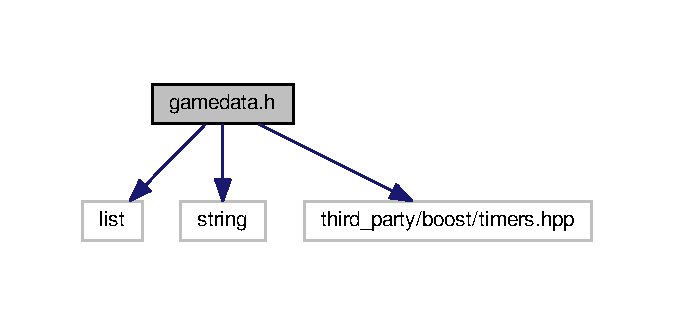
\includegraphics[width=324pt]{gamedata_8h__incl}
\end{center}
\end{figure}
이 그래프는 이 파일을 직/간접적으로 include 하는 파일들을 보여줍니다.\-:\nopagebreak
\begin{figure}[H]
\begin{center}
\leavevmode
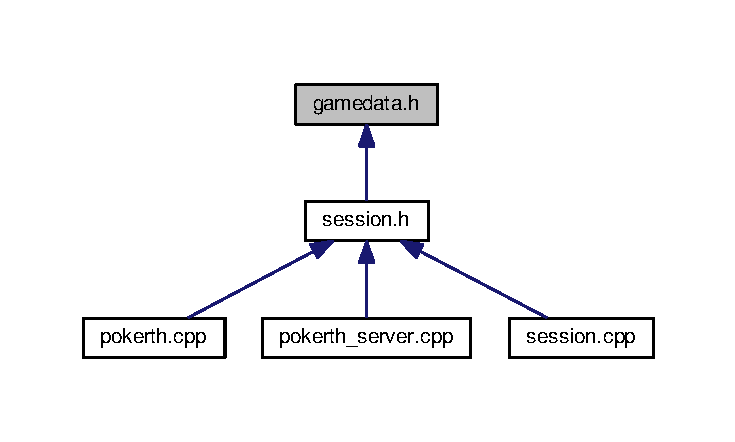
\includegraphics[width=350pt]{gamedata_8h__dep__incl}
\end{center}
\end{figure}
\subsection*{클래스}
\begin{DoxyCompactItemize}
\item 
struct \hyperlink{struct_game_data}{Game\-Data}
\item 
struct \hyperlink{struct_game_info}{Game\-Info}
\item 
struct \hyperlink{struct_start_data}{Start\-Data}
\item 
struct \hyperlink{struct_vote_kick_data}{Vote\-Kick\-Data}
\end{DoxyCompactItemize}
\subsection*{타입정의}
\begin{DoxyCompactItemize}
\item 
typedef std\-::list$<$ unsigned $>$ \hyperlink{gamedata_8h_a02ee63ca030dfa9d119c9f2df584e383}{Player\-Id\-List}
\end{DoxyCompactItemize}
\subsection*{열거형 타입}
\begin{DoxyCompactItemize}
\item 
enum \hyperlink{gamedata_8h_aaf5ef5a17b53e9997c837b07015589de}{Game\-Mode} \{ \hyperlink{gamedata_8h_aaf5ef5a17b53e9997c837b07015589dea5189be813705a7ad4b236a347c394328}{G\-A\-M\-E\-\_\-\-M\-O\-D\-E\-\_\-\-C\-R\-E\-A\-T\-E\-D} = 1, 
\hyperlink{gamedata_8h_aaf5ef5a17b53e9997c837b07015589dea8ea8a9a34b30d428601c025a651b4af3}{G\-A\-M\-E\-\_\-\-M\-O\-D\-E\-\_\-\-S\-T\-A\-R\-T\-E\-D}, 
\hyperlink{gamedata_8h_aaf5ef5a17b53e9997c837b07015589deaaeff0922a1bc9172b521c72d49835853}{G\-A\-M\-E\-\_\-\-M\-O\-D\-E\-\_\-\-C\-L\-O\-S\-E\-D}
 \}
\item 
enum \hyperlink{gamedata_8h_a86864855734edb7b2cb1efdc7a03fd57}{Game\-Type} \{ \hyperlink{gamedata_8h_a86864855734edb7b2cb1efdc7a03fd57a9b38699b42326665c8f890f41974dc79}{G\-A\-M\-E\-\_\-\-T\-Y\-P\-E\-\_\-\-N\-O\-R\-M\-A\-L} = 1, 
\hyperlink{gamedata_8h_a86864855734edb7b2cb1efdc7a03fd57a37614f35b98e12eb867d5de7d2438924}{G\-A\-M\-E\-\_\-\-T\-Y\-P\-E\-\_\-\-R\-E\-G\-I\-S\-T\-E\-R\-E\-D\-\_\-\-O\-N\-L\-Y}, 
\hyperlink{gamedata_8h_a86864855734edb7b2cb1efdc7a03fd57a8a108a1f08016faab6460576126e84b7}{G\-A\-M\-E\-\_\-\-T\-Y\-P\-E\-\_\-\-I\-N\-V\-I\-T\-E\-\_\-\-O\-N\-L\-Y}, 
\hyperlink{gamedata_8h_a86864855734edb7b2cb1efdc7a03fd57a24177b1bac68653c0a4246b9e112a3dc}{G\-A\-M\-E\-\_\-\-T\-Y\-P\-E\-\_\-\-R\-A\-N\-K\-I\-N\-G}
 \}
\item 
enum \hyperlink{gamedata_8h_a39f8de2f47cb4adf9038f5c6d6a8b8e6}{Raise\-Interval\-Mode} \{ \hyperlink{gamedata_8h_a39f8de2f47cb4adf9038f5c6d6a8b8e6a27cf82917dfcb27e20ee920f1158aff4}{R\-A\-I\-S\-E\-\_\-\-O\-N\-\_\-\-H\-A\-N\-D\-N\-U\-M\-B\-E\-R} = 1, 
\hyperlink{gamedata_8h_a39f8de2f47cb4adf9038f5c6d6a8b8e6a80ffd808e1ec5dd59052eab4c8ced488}{R\-A\-I\-S\-E\-\_\-\-O\-N\-\_\-\-M\-I\-N\-U\-T\-E\-S}
 \}
\item 
enum \hyperlink{gamedata_8h_a5532f34d7415bdfab60d67400cd5fc02}{Raise\-Mode} \{ \hyperlink{gamedata_8h_a5532f34d7415bdfab60d67400cd5fc02aec798914fb0781d6838679ab06926a56}{D\-O\-U\-B\-L\-E\-\_\-\-B\-L\-I\-N\-D\-S} = 1, 
\hyperlink{gamedata_8h_a5532f34d7415bdfab60d67400cd5fc02a6f7f1770289444177b4f5c36d2028fb3}{M\-A\-N\-U\-A\-L\-\_\-\-B\-L\-I\-N\-D\-S\-\_\-\-O\-R\-D\-E\-R}
 \}
\item 
enum \hyperlink{gamedata_8h_a250ebe9cdf4567798600e292202a66e6}{After\-Manual\-Blinds\-Mode} \{ \hyperlink{gamedata_8h_a250ebe9cdf4567798600e292202a66e6ac0e8cd440d7884b189fdb2e1a46aeebb}{A\-F\-T\-E\-R\-M\-B\-\_\-\-D\-O\-U\-B\-L\-E\-\_\-\-B\-L\-I\-N\-D\-S} = 1, 
\hyperlink{gamedata_8h_a250ebe9cdf4567798600e292202a66e6a28f19b2628a9c8720f5c23b3a68e809e}{A\-F\-T\-E\-R\-M\-B\-\_\-\-R\-A\-I\-S\-E\-\_\-\-A\-B\-O\-U\-T}, 
\hyperlink{gamedata_8h_a250ebe9cdf4567798600e292202a66e6a067261595087e84ba2c8bb772238c31a}{A\-F\-T\-E\-R\-M\-B\-\_\-\-S\-T\-A\-Y\-\_\-\-A\-T\-\_\-\-L\-A\-S\-T\-\_\-\-B\-L\-I\-N\-D}
 \}
\end{DoxyCompactItemize}


\subsection{타입정의 문서화}
\hypertarget{gamedata_8h_a02ee63ca030dfa9d119c9f2df584e383}{\index{gamedata.\-h@{gamedata.\-h}!Player\-Id\-List@{Player\-Id\-List}}
\index{Player\-Id\-List@{Player\-Id\-List}!gamedata.h@{gamedata.\-h}}
\subsubsection[{Player\-Id\-List}]{\setlength{\rightskip}{0pt plus 5cm}typedef std\-::list$<$unsigned$>$ {\bf Player\-Id\-List}}}\label{gamedata_8h_a02ee63ca030dfa9d119c9f2df584e383}


\subsection{열거형 타입 문서화}
\hypertarget{gamedata_8h_a250ebe9cdf4567798600e292202a66e6}{\index{gamedata.\-h@{gamedata.\-h}!After\-Manual\-Blinds\-Mode@{After\-Manual\-Blinds\-Mode}}
\index{After\-Manual\-Blinds\-Mode@{After\-Manual\-Blinds\-Mode}!gamedata.h@{gamedata.\-h}}
\subsubsection[{After\-Manual\-Blinds\-Mode}]{\setlength{\rightskip}{0pt plus 5cm}enum {\bf After\-Manual\-Blinds\-Mode}}}\label{gamedata_8h_a250ebe9cdf4567798600e292202a66e6}
\begin{Desc}
\item[열거형 멤버]\par
\begin{description}
\index{A\-F\-T\-E\-R\-M\-B\-\_\-\-D\-O\-U\-B\-L\-E\-\_\-\-B\-L\-I\-N\-D\-S@{A\-F\-T\-E\-R\-M\-B\-\_\-\-D\-O\-U\-B\-L\-E\-\_\-\-B\-L\-I\-N\-D\-S}!gamedata.\-h@{gamedata.\-h}}\index{gamedata.\-h@{gamedata.\-h}!A\-F\-T\-E\-R\-M\-B\-\_\-\-D\-O\-U\-B\-L\-E\-\_\-\-B\-L\-I\-N\-D\-S@{A\-F\-T\-E\-R\-M\-B\-\_\-\-D\-O\-U\-B\-L\-E\-\_\-\-B\-L\-I\-N\-D\-S}}\item[{\em 
\hypertarget{gamedata_8h_a250ebe9cdf4567798600e292202a66e6ac0e8cd440d7884b189fdb2e1a46aeebb}{A\-F\-T\-E\-R\-M\-B\-\_\-\-D\-O\-U\-B\-L\-E\-\_\-\-B\-L\-I\-N\-D\-S}\label{gamedata_8h_a250ebe9cdf4567798600e292202a66e6ac0e8cd440d7884b189fdb2e1a46aeebb}
}]\index{A\-F\-T\-E\-R\-M\-B\-\_\-\-R\-A\-I\-S\-E\-\_\-\-A\-B\-O\-U\-T@{A\-F\-T\-E\-R\-M\-B\-\_\-\-R\-A\-I\-S\-E\-\_\-\-A\-B\-O\-U\-T}!gamedata.\-h@{gamedata.\-h}}\index{gamedata.\-h@{gamedata.\-h}!A\-F\-T\-E\-R\-M\-B\-\_\-\-R\-A\-I\-S\-E\-\_\-\-A\-B\-O\-U\-T@{A\-F\-T\-E\-R\-M\-B\-\_\-\-R\-A\-I\-S\-E\-\_\-\-A\-B\-O\-U\-T}}\item[{\em 
\hypertarget{gamedata_8h_a250ebe9cdf4567798600e292202a66e6a28f19b2628a9c8720f5c23b3a68e809e}{A\-F\-T\-E\-R\-M\-B\-\_\-\-R\-A\-I\-S\-E\-\_\-\-A\-B\-O\-U\-T}\label{gamedata_8h_a250ebe9cdf4567798600e292202a66e6a28f19b2628a9c8720f5c23b3a68e809e}
}]\index{A\-F\-T\-E\-R\-M\-B\-\_\-\-S\-T\-A\-Y\-\_\-\-A\-T\-\_\-\-L\-A\-S\-T\-\_\-\-B\-L\-I\-N\-D@{A\-F\-T\-E\-R\-M\-B\-\_\-\-S\-T\-A\-Y\-\_\-\-A\-T\-\_\-\-L\-A\-S\-T\-\_\-\-B\-L\-I\-N\-D}!gamedata.\-h@{gamedata.\-h}}\index{gamedata.\-h@{gamedata.\-h}!A\-F\-T\-E\-R\-M\-B\-\_\-\-S\-T\-A\-Y\-\_\-\-A\-T\-\_\-\-L\-A\-S\-T\-\_\-\-B\-L\-I\-N\-D@{A\-F\-T\-E\-R\-M\-B\-\_\-\-S\-T\-A\-Y\-\_\-\-A\-T\-\_\-\-L\-A\-S\-T\-\_\-\-B\-L\-I\-N\-D}}\item[{\em 
\hypertarget{gamedata_8h_a250ebe9cdf4567798600e292202a66e6a067261595087e84ba2c8bb772238c31a}{A\-F\-T\-E\-R\-M\-B\-\_\-\-S\-T\-A\-Y\-\_\-\-A\-T\-\_\-\-L\-A\-S\-T\-\_\-\-B\-L\-I\-N\-D}\label{gamedata_8h_a250ebe9cdf4567798600e292202a66e6a067261595087e84ba2c8bb772238c31a}
}]\end{description}
\end{Desc}

\begin{DoxyCode}
67                            \{
68     \hyperlink{gamedata_8h_a250ebe9cdf4567798600e292202a66e6ac0e8cd440d7884b189fdb2e1a46aeebb}{AFTERMB\_DOUBLE\_BLINDS} = 1,
69     \hyperlink{gamedata_8h_a250ebe9cdf4567798600e292202a66e6a28f19b2628a9c8720f5c23b3a68e809e}{AFTERMB\_RAISE\_ABOUT},
70     \hyperlink{gamedata_8h_a250ebe9cdf4567798600e292202a66e6a067261595087e84ba2c8bb772238c31a}{AFTERMB\_STAY\_AT\_LAST\_BLIND}
71 \};
\end{DoxyCode}
\hypertarget{gamedata_8h_aaf5ef5a17b53e9997c837b07015589de}{\index{gamedata.\-h@{gamedata.\-h}!Game\-Mode@{Game\-Mode}}
\index{Game\-Mode@{Game\-Mode}!gamedata.h@{gamedata.\-h}}
\subsubsection[{Game\-Mode}]{\setlength{\rightskip}{0pt plus 5cm}enum {\bf Game\-Mode}}}\label{gamedata_8h_aaf5ef5a17b53e9997c837b07015589de}
\begin{Desc}
\item[열거형 멤버]\par
\begin{description}
\index{G\-A\-M\-E\-\_\-\-M\-O\-D\-E\-\_\-\-C\-R\-E\-A\-T\-E\-D@{G\-A\-M\-E\-\_\-\-M\-O\-D\-E\-\_\-\-C\-R\-E\-A\-T\-E\-D}!gamedata.\-h@{gamedata.\-h}}\index{gamedata.\-h@{gamedata.\-h}!G\-A\-M\-E\-\_\-\-M\-O\-D\-E\-\_\-\-C\-R\-E\-A\-T\-E\-D@{G\-A\-M\-E\-\_\-\-M\-O\-D\-E\-\_\-\-C\-R\-E\-A\-T\-E\-D}}\item[{\em 
\hypertarget{gamedata_8h_aaf5ef5a17b53e9997c837b07015589dea5189be813705a7ad4b236a347c394328}{G\-A\-M\-E\-\_\-\-M\-O\-D\-E\-\_\-\-C\-R\-E\-A\-T\-E\-D}\label{gamedata_8h_aaf5ef5a17b53e9997c837b07015589dea5189be813705a7ad4b236a347c394328}
}]\index{G\-A\-M\-E\-\_\-\-M\-O\-D\-E\-\_\-\-S\-T\-A\-R\-T\-E\-D@{G\-A\-M\-E\-\_\-\-M\-O\-D\-E\-\_\-\-S\-T\-A\-R\-T\-E\-D}!gamedata.\-h@{gamedata.\-h}}\index{gamedata.\-h@{gamedata.\-h}!G\-A\-M\-E\-\_\-\-M\-O\-D\-E\-\_\-\-S\-T\-A\-R\-T\-E\-D@{G\-A\-M\-E\-\_\-\-M\-O\-D\-E\-\_\-\-S\-T\-A\-R\-T\-E\-D}}\item[{\em 
\hypertarget{gamedata_8h_aaf5ef5a17b53e9997c837b07015589dea8ea8a9a34b30d428601c025a651b4af3}{G\-A\-M\-E\-\_\-\-M\-O\-D\-E\-\_\-\-S\-T\-A\-R\-T\-E\-D}\label{gamedata_8h_aaf5ef5a17b53e9997c837b07015589dea8ea8a9a34b30d428601c025a651b4af3}
}]\index{G\-A\-M\-E\-\_\-\-M\-O\-D\-E\-\_\-\-C\-L\-O\-S\-E\-D@{G\-A\-M\-E\-\_\-\-M\-O\-D\-E\-\_\-\-C\-L\-O\-S\-E\-D}!gamedata.\-h@{gamedata.\-h}}\index{gamedata.\-h@{gamedata.\-h}!G\-A\-M\-E\-\_\-\-M\-O\-D\-E\-\_\-\-C\-L\-O\-S\-E\-D@{G\-A\-M\-E\-\_\-\-M\-O\-D\-E\-\_\-\-C\-L\-O\-S\-E\-D}}\item[{\em 
\hypertarget{gamedata_8h_aaf5ef5a17b53e9997c837b07015589deaaeff0922a1bc9172b521c72d49835853}{G\-A\-M\-E\-\_\-\-M\-O\-D\-E\-\_\-\-C\-L\-O\-S\-E\-D}\label{gamedata_8h_aaf5ef5a17b53e9997c837b07015589deaaeff0922a1bc9172b521c72d49835853}
}]\end{description}
\end{Desc}

\begin{DoxyCode}
44               \{
45     \hyperlink{gamedata_8h_aaf5ef5a17b53e9997c837b07015589dea5189be813705a7ad4b236a347c394328}{GAME\_MODE\_CREATED} = 1,
46     \hyperlink{gamedata_8h_aaf5ef5a17b53e9997c837b07015589dea8ea8a9a34b30d428601c025a651b4af3}{GAME\_MODE\_STARTED},
47     \hyperlink{gamedata_8h_aaf5ef5a17b53e9997c837b07015589deaaeff0922a1bc9172b521c72d49835853}{GAME\_MODE\_CLOSED}
48 \};
\end{DoxyCode}
\hypertarget{gamedata_8h_a86864855734edb7b2cb1efdc7a03fd57}{\index{gamedata.\-h@{gamedata.\-h}!Game\-Type@{Game\-Type}}
\index{Game\-Type@{Game\-Type}!gamedata.h@{gamedata.\-h}}
\subsubsection[{Game\-Type}]{\setlength{\rightskip}{0pt plus 5cm}enum {\bf Game\-Type}}}\label{gamedata_8h_a86864855734edb7b2cb1efdc7a03fd57}
\begin{Desc}
\item[열거형 멤버]\par
\begin{description}
\index{G\-A\-M\-E\-\_\-\-T\-Y\-P\-E\-\_\-\-N\-O\-R\-M\-A\-L@{G\-A\-M\-E\-\_\-\-T\-Y\-P\-E\-\_\-\-N\-O\-R\-M\-A\-L}!gamedata.\-h@{gamedata.\-h}}\index{gamedata.\-h@{gamedata.\-h}!G\-A\-M\-E\-\_\-\-T\-Y\-P\-E\-\_\-\-N\-O\-R\-M\-A\-L@{G\-A\-M\-E\-\_\-\-T\-Y\-P\-E\-\_\-\-N\-O\-R\-M\-A\-L}}\item[{\em 
\hypertarget{gamedata_8h_a86864855734edb7b2cb1efdc7a03fd57a9b38699b42326665c8f890f41974dc79}{G\-A\-M\-E\-\_\-\-T\-Y\-P\-E\-\_\-\-N\-O\-R\-M\-A\-L}\label{gamedata_8h_a86864855734edb7b2cb1efdc7a03fd57a9b38699b42326665c8f890f41974dc79}
}]\index{G\-A\-M\-E\-\_\-\-T\-Y\-P\-E\-\_\-\-R\-E\-G\-I\-S\-T\-E\-R\-E\-D\-\_\-\-O\-N\-L\-Y@{G\-A\-M\-E\-\_\-\-T\-Y\-P\-E\-\_\-\-R\-E\-G\-I\-S\-T\-E\-R\-E\-D\-\_\-\-O\-N\-L\-Y}!gamedata.\-h@{gamedata.\-h}}\index{gamedata.\-h@{gamedata.\-h}!G\-A\-M\-E\-\_\-\-T\-Y\-P\-E\-\_\-\-R\-E\-G\-I\-S\-T\-E\-R\-E\-D\-\_\-\-O\-N\-L\-Y@{G\-A\-M\-E\-\_\-\-T\-Y\-P\-E\-\_\-\-R\-E\-G\-I\-S\-T\-E\-R\-E\-D\-\_\-\-O\-N\-L\-Y}}\item[{\em 
\hypertarget{gamedata_8h_a86864855734edb7b2cb1efdc7a03fd57a37614f35b98e12eb867d5de7d2438924}{G\-A\-M\-E\-\_\-\-T\-Y\-P\-E\-\_\-\-R\-E\-G\-I\-S\-T\-E\-R\-E\-D\-\_\-\-O\-N\-L\-Y}\label{gamedata_8h_a86864855734edb7b2cb1efdc7a03fd57a37614f35b98e12eb867d5de7d2438924}
}]\index{G\-A\-M\-E\-\_\-\-T\-Y\-P\-E\-\_\-\-I\-N\-V\-I\-T\-E\-\_\-\-O\-N\-L\-Y@{G\-A\-M\-E\-\_\-\-T\-Y\-P\-E\-\_\-\-I\-N\-V\-I\-T\-E\-\_\-\-O\-N\-L\-Y}!gamedata.\-h@{gamedata.\-h}}\index{gamedata.\-h@{gamedata.\-h}!G\-A\-M\-E\-\_\-\-T\-Y\-P\-E\-\_\-\-I\-N\-V\-I\-T\-E\-\_\-\-O\-N\-L\-Y@{G\-A\-M\-E\-\_\-\-T\-Y\-P\-E\-\_\-\-I\-N\-V\-I\-T\-E\-\_\-\-O\-N\-L\-Y}}\item[{\em 
\hypertarget{gamedata_8h_a86864855734edb7b2cb1efdc7a03fd57a8a108a1f08016faab6460576126e84b7}{G\-A\-M\-E\-\_\-\-T\-Y\-P\-E\-\_\-\-I\-N\-V\-I\-T\-E\-\_\-\-O\-N\-L\-Y}\label{gamedata_8h_a86864855734edb7b2cb1efdc7a03fd57a8a108a1f08016faab6460576126e84b7}
}]\index{G\-A\-M\-E\-\_\-\-T\-Y\-P\-E\-\_\-\-R\-A\-N\-K\-I\-N\-G@{G\-A\-M\-E\-\_\-\-T\-Y\-P\-E\-\_\-\-R\-A\-N\-K\-I\-N\-G}!gamedata.\-h@{gamedata.\-h}}\index{gamedata.\-h@{gamedata.\-h}!G\-A\-M\-E\-\_\-\-T\-Y\-P\-E\-\_\-\-R\-A\-N\-K\-I\-N\-G@{G\-A\-M\-E\-\_\-\-T\-Y\-P\-E\-\_\-\-R\-A\-N\-K\-I\-N\-G}}\item[{\em 
\hypertarget{gamedata_8h_a86864855734edb7b2cb1efdc7a03fd57a24177b1bac68653c0a4246b9e112a3dc}{G\-A\-M\-E\-\_\-\-T\-Y\-P\-E\-\_\-\-R\-A\-N\-K\-I\-N\-G}\label{gamedata_8h_a86864855734edb7b2cb1efdc7a03fd57a24177b1bac68653c0a4246b9e112a3dc}
}]\end{description}
\end{Desc}

\begin{DoxyCode}
50               \{
51     \hyperlink{gamedata_8h_a86864855734edb7b2cb1efdc7a03fd57a9b38699b42326665c8f890f41974dc79}{GAME\_TYPE\_NORMAL} = 1,
52     \hyperlink{gamedata_8h_a86864855734edb7b2cb1efdc7a03fd57a37614f35b98e12eb867d5de7d2438924}{GAME\_TYPE\_REGISTERED\_ONLY},
53     \hyperlink{gamedata_8h_a86864855734edb7b2cb1efdc7a03fd57a8a108a1f08016faab6460576126e84b7}{GAME\_TYPE\_INVITE\_ONLY},
54     \hyperlink{gamedata_8h_a86864855734edb7b2cb1efdc7a03fd57a24177b1bac68653c0a4246b9e112a3dc}{GAME\_TYPE\_RANKING}
55 \};
\end{DoxyCode}
\hypertarget{gamedata_8h_a39f8de2f47cb4adf9038f5c6d6a8b8e6}{\index{gamedata.\-h@{gamedata.\-h}!Raise\-Interval\-Mode@{Raise\-Interval\-Mode}}
\index{Raise\-Interval\-Mode@{Raise\-Interval\-Mode}!gamedata.h@{gamedata.\-h}}
\subsubsection[{Raise\-Interval\-Mode}]{\setlength{\rightskip}{0pt plus 5cm}enum {\bf Raise\-Interval\-Mode}}}\label{gamedata_8h_a39f8de2f47cb4adf9038f5c6d6a8b8e6}
\begin{Desc}
\item[열거형 멤버]\par
\begin{description}
\index{R\-A\-I\-S\-E\-\_\-\-O\-N\-\_\-\-H\-A\-N\-D\-N\-U\-M\-B\-E\-R@{R\-A\-I\-S\-E\-\_\-\-O\-N\-\_\-\-H\-A\-N\-D\-N\-U\-M\-B\-E\-R}!gamedata.\-h@{gamedata.\-h}}\index{gamedata.\-h@{gamedata.\-h}!R\-A\-I\-S\-E\-\_\-\-O\-N\-\_\-\-H\-A\-N\-D\-N\-U\-M\-B\-E\-R@{R\-A\-I\-S\-E\-\_\-\-O\-N\-\_\-\-H\-A\-N\-D\-N\-U\-M\-B\-E\-R}}\item[{\em 
\hypertarget{gamedata_8h_a39f8de2f47cb4adf9038f5c6d6a8b8e6a27cf82917dfcb27e20ee920f1158aff4}{R\-A\-I\-S\-E\-\_\-\-O\-N\-\_\-\-H\-A\-N\-D\-N\-U\-M\-B\-E\-R}\label{gamedata_8h_a39f8de2f47cb4adf9038f5c6d6a8b8e6a27cf82917dfcb27e20ee920f1158aff4}
}]\index{R\-A\-I\-S\-E\-\_\-\-O\-N\-\_\-\-M\-I\-N\-U\-T\-E\-S@{R\-A\-I\-S\-E\-\_\-\-O\-N\-\_\-\-M\-I\-N\-U\-T\-E\-S}!gamedata.\-h@{gamedata.\-h}}\index{gamedata.\-h@{gamedata.\-h}!R\-A\-I\-S\-E\-\_\-\-O\-N\-\_\-\-M\-I\-N\-U\-T\-E\-S@{R\-A\-I\-S\-E\-\_\-\-O\-N\-\_\-\-M\-I\-N\-U\-T\-E\-S}}\item[{\em 
\hypertarget{gamedata_8h_a39f8de2f47cb4adf9038f5c6d6a8b8e6a80ffd808e1ec5dd59052eab4c8ced488}{R\-A\-I\-S\-E\-\_\-\-O\-N\-\_\-\-M\-I\-N\-U\-T\-E\-S}\label{gamedata_8h_a39f8de2f47cb4adf9038f5c6d6a8b8e6a80ffd808e1ec5dd59052eab4c8ced488}
}]\end{description}
\end{Desc}

\begin{DoxyCode}
57                        \{
58     \hyperlink{gamedata_8h_a39f8de2f47cb4adf9038f5c6d6a8b8e6a27cf82917dfcb27e20ee920f1158aff4}{RAISE\_ON\_HANDNUMBER} = 1,
59     \hyperlink{gamedata_8h_a39f8de2f47cb4adf9038f5c6d6a8b8e6a80ffd808e1ec5dd59052eab4c8ced488}{RAISE\_ON\_MINUTES}
60 \};
\end{DoxyCode}
\hypertarget{gamedata_8h_a5532f34d7415bdfab60d67400cd5fc02}{\index{gamedata.\-h@{gamedata.\-h}!Raise\-Mode@{Raise\-Mode}}
\index{Raise\-Mode@{Raise\-Mode}!gamedata.h@{gamedata.\-h}}
\subsubsection[{Raise\-Mode}]{\setlength{\rightskip}{0pt plus 5cm}enum {\bf Raise\-Mode}}}\label{gamedata_8h_a5532f34d7415bdfab60d67400cd5fc02}
\begin{Desc}
\item[열거형 멤버]\par
\begin{description}
\index{D\-O\-U\-B\-L\-E\-\_\-\-B\-L\-I\-N\-D\-S@{D\-O\-U\-B\-L\-E\-\_\-\-B\-L\-I\-N\-D\-S}!gamedata.\-h@{gamedata.\-h}}\index{gamedata.\-h@{gamedata.\-h}!D\-O\-U\-B\-L\-E\-\_\-\-B\-L\-I\-N\-D\-S@{D\-O\-U\-B\-L\-E\-\_\-\-B\-L\-I\-N\-D\-S}}\item[{\em 
\hypertarget{gamedata_8h_a5532f34d7415bdfab60d67400cd5fc02aec798914fb0781d6838679ab06926a56}{D\-O\-U\-B\-L\-E\-\_\-\-B\-L\-I\-N\-D\-S}\label{gamedata_8h_a5532f34d7415bdfab60d67400cd5fc02aec798914fb0781d6838679ab06926a56}
}]\index{M\-A\-N\-U\-A\-L\-\_\-\-B\-L\-I\-N\-D\-S\-\_\-\-O\-R\-D\-E\-R@{M\-A\-N\-U\-A\-L\-\_\-\-B\-L\-I\-N\-D\-S\-\_\-\-O\-R\-D\-E\-R}!gamedata.\-h@{gamedata.\-h}}\index{gamedata.\-h@{gamedata.\-h}!M\-A\-N\-U\-A\-L\-\_\-\-B\-L\-I\-N\-D\-S\-\_\-\-O\-R\-D\-E\-R@{M\-A\-N\-U\-A\-L\-\_\-\-B\-L\-I\-N\-D\-S\-\_\-\-O\-R\-D\-E\-R}}\item[{\em 
\hypertarget{gamedata_8h_a5532f34d7415bdfab60d67400cd5fc02a6f7f1770289444177b4f5c36d2028fb3}{M\-A\-N\-U\-A\-L\-\_\-\-B\-L\-I\-N\-D\-S\-\_\-\-O\-R\-D\-E\-R}\label{gamedata_8h_a5532f34d7415bdfab60d67400cd5fc02a6f7f1770289444177b4f5c36d2028fb3}
}]\end{description}
\end{Desc}

\begin{DoxyCode}
62                \{
63     \hyperlink{gamedata_8h_a5532f34d7415bdfab60d67400cd5fc02aec798914fb0781d6838679ab06926a56}{DOUBLE\_BLINDS} = 1,
64     \hyperlink{gamedata_8h_a5532f34d7415bdfab60d67400cd5fc02a6f7f1770289444177b4f5c36d2028fb3}{MANUAL\_BLINDS\_ORDER}
65 \};
\end{DoxyCode}

\hypertarget{load_8cpp}{\section{load.\-cpp 파일 참조}
\label{load_8cpp}\index{load.\-cpp@{load.\-cpp}}
}
{\ttfamily \#include $<$third\-\_\-party/asn1/\-Poker\-T\-H\-Message.\-h$>$}\\*
{\ttfamily \#include $<$boost/program\-\_\-options.\-hpp$>$}\\*
{\ttfamily \#include $<$boost/asio.\-hpp$>$}\\*
{\ttfamily \#include $<$boost/thread.\-hpp$>$}\\*
{\ttfamily \#include $<$gsasl.\-h$>$}\\*
{\ttfamily \#include $<$iostream$>$}\\*
{\ttfamily \#include $<$sstream$>$}\\*
load.\-cpp에 대한 include 의존 그래프\nopagebreak
\begin{figure}[H]
\begin{center}
\leavevmode
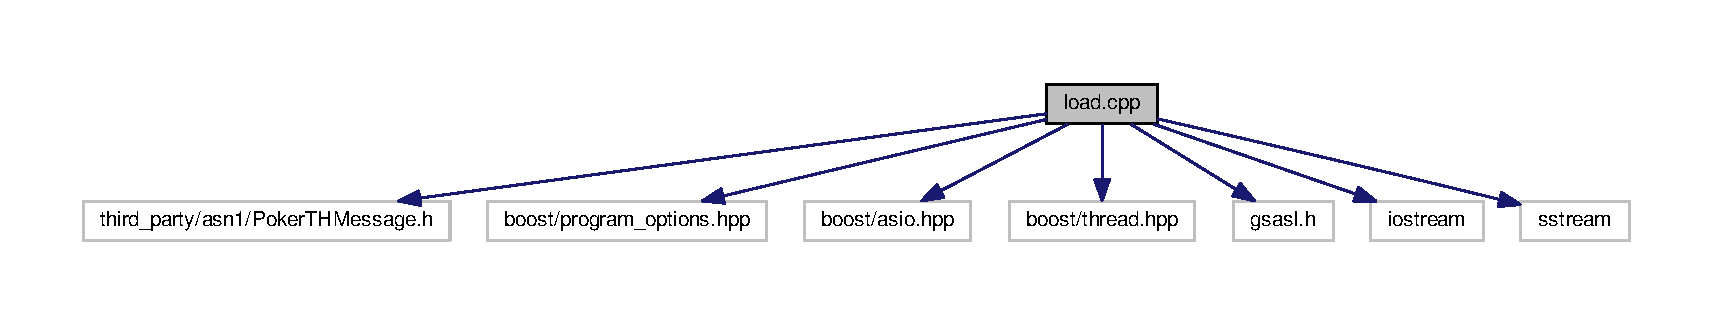
\includegraphics[width=350pt]{load_8cpp__incl}
\end{center}
\end{figure}
\subsection*{클래스}
\begin{DoxyCompactItemize}
\item 
struct \hyperlink{struct_net_session}{Net\-Session}
\end{DoxyCompactItemize}
\subsection*{매크로}
\begin{DoxyCompactItemize}
\item 
\#define \hyperlink{load_8cpp_a5cf0d6cbdffe082b37d1b816690cc62c}{S\-T\-L\-\_\-\-S\-T\-R\-I\-N\-G\-\_\-\-F\-R\-O\-M\-\_\-\-O\-C\-T\-E\-T\-\_\-\-S\-T\-R\-I\-N\-G}(\-\_\-a)~(string((const char $\ast$)(\-\_\-a).buf, (\-\_\-a).size))
\item 
\#define \hyperlink{load_8cpp_a6821bafc3c88dfb2e433a095df9940c6}{B\-U\-F\-\_\-\-S\-I\-Z\-E}~1024
\end{DoxyCompactItemize}
\subsection*{함수}
\begin{DoxyCompactItemize}
\item 
static int \hyperlink{load_8cpp_a3648412ef7ef48b734fad6e3be1ff5c0}{net\-\_\-packet\-\_\-print\-\_\-to\-\_\-string} (const void $\ast$buffer, size\-\_\-t size, void $\ast$packet\-Str)
\item 
Poker\-T\-H\-Message\-\_\-t $\ast$ \hyperlink{load_8cpp_ab7e9bb8e3de485508865004717ac33cd}{receive\-Message} (\hyperlink{struct_net_session}{Net\-Session} $\ast$session)
\item 
bool \hyperlink{load_8cpp_a147f7872930fe5e0da14572d9bf42100}{send\-Message} (\hyperlink{struct_net_session}{Net\-Session} $\ast$session, Poker\-T\-H\-Message\-\_\-t $\ast$msg)
\item 
int \hyperlink{load_8cpp_a0ddf1224851353fc92bfbff6f499fa97}{main} (int argc, char $\ast$argv\mbox{[}$\,$\mbox{]})
\end{DoxyCompactItemize}


\subsection{매크로 문서화}
\hypertarget{load_8cpp_a6821bafc3c88dfb2e433a095df9940c6}{\index{load.\-cpp@{load.\-cpp}!B\-U\-F\-\_\-\-S\-I\-Z\-E@{B\-U\-F\-\_\-\-S\-I\-Z\-E}}
\index{B\-U\-F\-\_\-\-S\-I\-Z\-E@{B\-U\-F\-\_\-\-S\-I\-Z\-E}!load.cpp@{load.\-cpp}}
\subsubsection[{B\-U\-F\-\_\-\-S\-I\-Z\-E}]{\setlength{\rightskip}{0pt plus 5cm}\#define B\-U\-F\-\_\-\-S\-I\-Z\-E~1024}}\label{load_8cpp_a6821bafc3c88dfb2e433a095df9940c6}
\hypertarget{load_8cpp_a5cf0d6cbdffe082b37d1b816690cc62c}{\index{load.\-cpp@{load.\-cpp}!S\-T\-L\-\_\-\-S\-T\-R\-I\-N\-G\-\_\-\-F\-R\-O\-M\-\_\-\-O\-C\-T\-E\-T\-\_\-\-S\-T\-R\-I\-N\-G@{S\-T\-L\-\_\-\-S\-T\-R\-I\-N\-G\-\_\-\-F\-R\-O\-M\-\_\-\-O\-C\-T\-E\-T\-\_\-\-S\-T\-R\-I\-N\-G}}
\index{S\-T\-L\-\_\-\-S\-T\-R\-I\-N\-G\-\_\-\-F\-R\-O\-M\-\_\-\-O\-C\-T\-E\-T\-\_\-\-S\-T\-R\-I\-N\-G@{S\-T\-L\-\_\-\-S\-T\-R\-I\-N\-G\-\_\-\-F\-R\-O\-M\-\_\-\-O\-C\-T\-E\-T\-\_\-\-S\-T\-R\-I\-N\-G}!load.cpp@{load.\-cpp}}
\subsubsection[{S\-T\-L\-\_\-\-S\-T\-R\-I\-N\-G\-\_\-\-F\-R\-O\-M\-\_\-\-O\-C\-T\-E\-T\-\_\-\-S\-T\-R\-I\-N\-G}]{\setlength{\rightskip}{0pt plus 5cm}\#define S\-T\-L\-\_\-\-S\-T\-R\-I\-N\-G\-\_\-\-F\-R\-O\-M\-\_\-\-O\-C\-T\-E\-T\-\_\-\-S\-T\-R\-I\-N\-G(
\begin{DoxyParamCaption}
\item[{}]{\-\_\-a}
\end{DoxyParamCaption}
)~(string((const char $\ast$)(\-\_\-a).buf, (\-\_\-a).size))}}\label{load_8cpp_a5cf0d6cbdffe082b37d1b816690cc62c}


\subsection{함수 문서화}
\hypertarget{load_8cpp_a0ddf1224851353fc92bfbff6f499fa97}{\index{load.\-cpp@{load.\-cpp}!main@{main}}
\index{main@{main}!load.cpp@{load.\-cpp}}
\subsubsection[{main}]{\setlength{\rightskip}{0pt plus 5cm}int main (
\begin{DoxyParamCaption}
\item[{int}]{argc, }
\item[{char $\ast$}]{argv\mbox{[}$\,$\mbox{]}}
\end{DoxyParamCaption}
)}}\label{load_8cpp_a0ddf1224851353fc92bfbff6f499fa97}

\begin{DoxyCode}
120 \{
121     \textcolor{keywordflow}{try} \{
122         \textcolor{comment}{// Check command line options.}
123         po::options\_description desc(\textcolor{stringliteral}{"Allowed options"});
124         desc.add\_options()
125         (\textcolor{stringliteral}{"help,h"}, \textcolor{stringliteral}{"produce help message"})
126         (\textcolor{stringliteral}{"server,s"}, po::value<string>(), \textcolor{stringliteral}{"PokerTH server name"})
127         (\textcolor{stringliteral}{"port,P"}, po::value<string>(), \textcolor{stringliteral}{"PokerTH server port"})
128         (\textcolor{stringliteral}{"numGames,n"}, po::value<unsigned>(), \textcolor{stringliteral}{"Number of games to open"})
129         (\textcolor{stringliteral}{"firstId,f"}, po::value<int>(), \textcolor{stringliteral}{"First id of username testx"})
130         ;
131 
132         po::variables\_map vm;
133         po::store(po::parse\_command\_line(argc, argv, desc), vm);
134         po::notify(vm);
135 
136         \textcolor{keywordflow}{if} (vm.count(\textcolor{stringliteral}{"help"})) \{
137             cout << desc << endl;
138             \textcolor{keywordflow}{return} 1;
139         \}
140         \textcolor{keywordflow}{if} (!vm.count(\textcolor{stringliteral}{"server"}) || !vm.count(\textcolor{stringliteral}{"port"}) || !vm.count(\textcolor{stringliteral}{"numGames"}) || !vm.count(\textcolor{stringliteral}{"firstId"})) \{
141             cout << \textcolor{stringliteral}{"Missing option!"} << endl << desc << endl;
142             \textcolor{keywordflow}{return} 1;
143         \}
144 
145         \textcolor{keywordtype}{string} server(vm[\textcolor{stringliteral}{"server"}].as<string>());
146         \textcolor{keywordtype}{string} port = vm[\textcolor{stringliteral}{"port"}].as<\textcolor{keywordtype}{string}>();
147         \textcolor{keywordtype}{unsigned} numGames = vm[\textcolor{stringliteral}{"numGames"}].as<\textcolor{keywordtype}{unsigned}>();
148         \textcolor{keywordtype}{int} firstId = vm[\textcolor{stringliteral}{"firstId"}].as<\textcolor{keywordtype}{int}>();
149 
150         \textcolor{comment}{// Initialise gsasl.}
151         Gsasl *authContext;
152         \textcolor{keywordtype}{int} res = gsasl\_init(&authContext);
153         \textcolor{keywordflow}{if} (res != GSASL\_OK) \{
154             cout << \textcolor{stringliteral}{"gsasl init failed"} << endl;
155             \textcolor{keywordflow}{return} 1;
156         \}
157 
158         \textcolor{keywordflow}{if} (!gsasl\_client\_support\_p(authContext, \textcolor{stringliteral}{"SCRAM-SHA-1"})) \{
159             gsasl\_done(authContext);
160             cout << \textcolor{stringliteral}{"This version of gsasl does not support SCRAM-SHA-1"} << endl;
161             \textcolor{keywordflow}{return} 1;
162         \}
163 
164         \textcolor{comment}{// Connect to the PokerTH server.}
165         boost::asio::io\_service ioService;
166         tcp::resolver resolver(ioService);
167         tcp::resolver::query query(server, port);
168         tcp::resolver::iterator endpoint\_iterator = resolver.resolve(query);
169         tcp::resolver::iterator end;
170         boost::system::error\_code error = boost::asio::error::host\_not\_found;
171         tcp::resolver::iterator curEndpoint;
172         tcp::socket tmpSocket(ioService);
173         \textcolor{keywordflow}{while} (error && endpoint\_iterator != end) \{
174             curEndpoint = endpoint\_iterator++;
175             tmpSocket.connect(*curEndpoint, error);
176             tmpSocket.close();
177         \}
178 
179         \textcolor{keywordflow}{if} (error) \{
180             cout << \textcolor{stringliteral}{"Connect failed"} << endl;
181             \textcolor{keywordflow}{return} 1;
182         \}
183 
184         PokerTHMessage\_t *msg = NULL;
185         \textcolor{keywordtype}{int} errorCode;
186         \textcolor{keywordtype}{char} *tmpOut;
187         \textcolor{keywordtype}{size\_t} tmpOutSize;
188         \textcolor{keywordtype}{string} nextGsaslMsg;
189         \hyperlink{struct_net_session}{NetSession} **sessionArray = \textcolor{keyword}{new} \hyperlink{struct_net_session}{NetSession} *[numGames * 10];
190         \textcolor{keywordtype}{unsigned} *gameId = \textcolor{keyword}{new} \textcolor{keywordtype}{unsigned}[numGames];
191         \textcolor{keyword}{const} \textcolor{keywordtype}{int} LoginsPerLoop = 50;
192         \textcolor{keywordflow}{for} (\textcolor{keywordtype}{int} t = 0; t < (numGames * 10) / LoginsPerLoop + 1; t++) \{
193             \textcolor{keywordtype}{int} startNum = t * LoginsPerLoop;
194             \textcolor{keywordtype}{int} endNum = (t + 1) * LoginsPerLoop;
195             \textcolor{keywordflow}{if} (endNum > numGames * 10) \{
196                 endNum = numGames * 10;
197             \}
198             \textcolor{keywordflow}{for} (\textcolor{keywordtype}{int} i = startNum; i < endNum; i++) \{
199                 sessionArray[i] = \textcolor{keyword}{new} \hyperlink{struct_net_session}{NetSession}(ioService);
200                 \hyperlink{struct_net_session}{NetSession} *session = sessionArray[i];
201 
202                 session->\hyperlink{struct_net_session_a93ead5e6efef575fd61ed0514100310b}{socket}.connect(*curEndpoint, error);
203 
204                 \textcolor{comment}{// Receive server information}
205                 msg = \hyperlink{load_8cpp_ab7e9bb8e3de485508865004717ac33cd}{receiveMessage}(session);
206                 \textcolor{keywordflow}{if} (!msg || msg->present != PokerTHMessage\_PR\_announceMessage) \{
207                     cout << \textcolor{stringliteral}{"Announce failed"} << endl;
208                     \textcolor{keywordflow}{return} 1;
209                 \}
210                 ASN\_STRUCT\_FREE(asn\_DEF\_PokerTHMessage, msg);
211 
212                 \textcolor{comment}{// Send init}
213                 msg = (PokerTHMessage\_t *)calloc(1, \textcolor{keyword}{sizeof}(PokerTHMessage\_t));
214                 msg->present = PokerTHMessage\_PR\_initMessage;
215                 InitMessage\_t *netInit = &msg->choice.initMessage;
216                 netInit->requestedVersion.major = 2;
217                 netInit->requestedVersion.minor = 0;
218                 errorCode = gsasl\_client\_start(authContext, \textcolor{stringliteral}{"SCRAM-SHA-1"}, &session->
      \hyperlink{struct_net_session_a633af90850d032509cfa243abb6898a8}{authSession});
219                 \textcolor{keywordflow}{if} (errorCode != GSASL\_OK) \{
220                     cout << \textcolor{stringliteral}{"Auth start error."} << endl;
221                     \textcolor{keywordflow}{return} 1;
222                 \}
223                 ostringstream param;
224                 param << \textcolor{stringliteral}{"test"} << i + firstId;
225                 cout << \textcolor{stringliteral}{"User "} << param.str() << \textcolor{stringliteral}{" logging in."} << endl;
226                 session->\hyperlink{struct_net_session_aec0bfb7bd042d9f19df3fc91dd8accae}{name} = param.str();
227                 gsasl\_property\_set(session->\hyperlink{struct_net_session_a633af90850d032509cfa243abb6898a8}{authSession}, GSASL\_AUTHID, session->
      \hyperlink{struct_net_session_aec0bfb7bd042d9f19df3fc91dd8accae}{name}.c\_str());
228                 gsasl\_property\_set(session->\hyperlink{struct_net_session_a633af90850d032509cfa243abb6898a8}{authSession}, GSASL\_PASSWORD, session->
      \hyperlink{struct_net_session_aec0bfb7bd042d9f19df3fc91dd8accae}{name}.c\_str());
229 
230                 netInit->login.present = login\_PR\_authenticatedLogin;
231                 AuthenticatedLogin\_t *authLogin = &netInit->login.choice.authenticatedLogin;
232 
233                 errorCode = gsasl\_step(session->\hyperlink{struct_net_session_a633af90850d032509cfa243abb6898a8}{authSession}, NULL, 0, &tmpOut, &tmpOutSize);
234                 \textcolor{keywordflow}{if} (errorCode == GSASL\_NEEDS\_MORE) \{
235                     nextGsaslMsg = string(tmpOut, tmpOutSize);
236                 \} \textcolor{keywordflow}{else} \{
237                     cout << \textcolor{stringliteral}{"gsasl step 1 failed"} << endl;
238                     \textcolor{keywordflow}{return} 1;
239                 \}
240                 gsasl\_free(tmpOut);
241 
242                 OCTET\_STRING\_fromBuf(&authLogin->clientUserData,
243                                      nextGsaslMsg.c\_str(),
244                                      nextGsaslMsg.length());
245                 \textcolor{keywordflow}{if} (!\hyperlink{load_8cpp_a147f7872930fe5e0da14572d9bf42100}{sendMessage}(session, msg)) \{
246                     cout << \textcolor{stringliteral}{"Init auth request failed"} << endl;
247                     \textcolor{keywordflow}{return} 1;
248                 \}
249             \}
250 
251             \textcolor{keywordflow}{for} (\textcolor{keywordtype}{int} i = startNum; i < endNum; i++) \{
252                 \hyperlink{struct_net_session}{NetSession} *session = sessionArray[i];
253                 msg = \hyperlink{load_8cpp_ab7e9bb8e3de485508865004717ac33cd}{receiveMessage}(session);
254                 \textcolor{keywordflow}{if} (!msg || msg->present != PokerTHMessage\_PR\_authMessage) \{
255                     cout << \textcolor{stringliteral}{"Auth request failed"} << endl;
256                     \textcolor{keywordflow}{return} 1;
257                 \}
258 
259                 AuthMessage\_t *netAuth = &msg->choice.authMessage;
260                 AuthServerChallenge\_t *netChallenge = &netAuth->choice.authServerChallenge;
261                 \textcolor{keywordtype}{string} challengeStr = \hyperlink{load_8cpp_a5cf0d6cbdffe082b37d1b816690cc62c}{STL\_STRING\_FROM\_OCTET\_STRING}(netChallenge
      ->serverChallenge);
262                 errorCode = gsasl\_step(session->\hyperlink{struct_net_session_a633af90850d032509cfa243abb6898a8}{authSession}, challengeStr.c\_str(), challengeStr.
      size(), &tmpOut, &tmpOutSize);
263                 \textcolor{keywordflow}{if} (errorCode == GSASL\_NEEDS\_MORE) \{
264                     nextGsaslMsg = string(tmpOut, tmpOutSize);
265                 \} \textcolor{keywordflow}{else} \{
266                     cout << \textcolor{stringliteral}{"gsasl step 2 failed"} << endl;
267                     \textcolor{keywordflow}{return} 1;
268                 \}
269                 gsasl\_free(tmpOut);
270                 ASN\_STRUCT\_FREE(asn\_DEF\_PokerTHMessage, msg);
271                 msg = (PokerTHMessage\_t *)calloc(1, \textcolor{keyword}{sizeof}(PokerTHMessage\_t));
272                 msg->present = PokerTHMessage\_PR\_authMessage;
273                 AuthMessage\_t *outAuth = &msg->choice.authMessage;
274                 outAuth->present = AuthMessage\_PR\_authClientResponse;
275                 AuthClientResponse\_t *outResponse = &outAuth->choice.authClientResponse;
276 
277                 OCTET\_STRING\_fromBuf(&outResponse->clientResponse,
278                                      nextGsaslMsg.c\_str(),
279                                      nextGsaslMsg.length());
280                 \textcolor{keywordflow}{if} (!\hyperlink{load_8cpp_a147f7872930fe5e0da14572d9bf42100}{sendMessage}(session, msg)) \{
281                     cout << \textcolor{stringliteral}{"Init auth response failed"} << endl;
282                     \textcolor{keywordflow}{return} 1;
283                 \}
284             \}
285 
286             \textcolor{keywordflow}{for} (\textcolor{keywordtype}{int} i = startNum; i < endNum; i++) \{
287                 \hyperlink{struct_net_session}{NetSession} *session = sessionArray[i];
288                 msg = \hyperlink{load_8cpp_ab7e9bb8e3de485508865004717ac33cd}{receiveMessage}(session);
289                 \textcolor{keywordflow}{if} (!msg || msg->present != PokerTHMessage\_PR\_authMessage) \{
290                     cout << \textcolor{stringliteral}{"Auth response failed"} << endl;
291                     \textcolor{keywordflow}{return} 1;
292                 \}
293                 ASN\_STRUCT\_FREE(asn\_DEF\_PokerTHMessage, msg);
294 
295                 \textcolor{comment}{// Receive init ack}
296                 msg = \hyperlink{load_8cpp_ab7e9bb8e3de485508865004717ac33cd}{receiveMessage}(session);
297                 \textcolor{keywordflow}{if} (!msg || msg->present != PokerTHMessage\_PR\_initAckMessage) \{
298                     cout << \textcolor{stringliteral}{"Init ack failed"} << endl;
299                     \textcolor{keywordflow}{return} 1;
300                 \}
301                 ASN\_STRUCT\_FREE(asn\_DEF\_PokerTHMessage, msg);
302 
303                 \textcolor{keywordflow}{for} (\textcolor{keywordtype}{int} j = i; j >= 0; j--) \{
304                     \textcolor{keywordtype}{size\_t} bytes\_readable = sessionArray[j]->\hyperlink{struct_net_session_a93ead5e6efef575fd61ed0514100310b}{socket}.available();
305                     \textcolor{keywordflow}{while} (bytes\_readable > 0) \{
306                         msg = \hyperlink{load_8cpp_ab7e9bb8e3de485508865004717ac33cd}{receiveMessage}(sessionArray[j]);
307                         ASN\_STRUCT\_FREE(asn\_DEF\_PokerTHMessage, msg);
308                         bytes\_readable = sessionArray[j]->\hyperlink{struct_net_session_a93ead5e6efef575fd61ed0514100310b}{socket}.available();
309                     \}
310                 \}
311             \}
312         \}
313 
314         \textcolor{keywordflow}{for} (\textcolor{keywordtype}{int} g = 0; g < numGames; g++) \{
315             \hyperlink{struct_net_session}{NetSession} *session = sessionArray[g * 10];
316             \textcolor{comment}{// Send create game}
317             cout << \textcolor{stringliteral}{"Player "} << session->\hyperlink{struct_net_session_aec0bfb7bd042d9f19df3fc91dd8accae}{name} << \textcolor{stringliteral}{" creating game "} << g+1 << endl;
318             msg = (PokerTHMessage\_t *)calloc(1, \textcolor{keyword}{sizeof}(PokerTHMessage\_t));
319             msg->present = PokerTHMessage\_PR\_joinGameRequestMessage;
320             JoinGameRequestMessage\_t *netJoinGame = &msg->choice.joinGameRequestMessage;
321             \textcolor{keywordtype}{string} tmpGamePassword(\textcolor{stringliteral}{"blah123"});
322             netJoinGame->password = OCTET\_STRING\_new\_fromBuf(
323                                         &asn\_DEF\_UTF8String,
324                                         tmpGamePassword.c\_str(),
325                                         tmpGamePassword.length());
326             netJoinGame->joinGameAction.present = joinGameAction\_PR\_joinNewGame;
327             JoinNewGame\_t *joinNew = &netJoinGame->joinGameAction.choice.joinNewGame;
328             \textcolor{keywordtype}{string} tmpGameName(\textcolor{stringliteral}{"\_loadtest\_do\_not\_join\_"} + session->\hyperlink{struct_net_session_aec0bfb7bd042d9f19df3fc91dd8accae}{name});
329             joinNew->gameInfo.netGameType       = netGameType\_normalGame;
330             joinNew->gameInfo.maxNumPlayers     = 10;
331             joinNew->gameInfo.raiseIntervalMode.present = raiseIntervalMode\_PR\_raiseEveryHands;
332             joinNew->gameInfo.raiseIntervalMode.choice.raiseEveryHands = 1;
333             joinNew->gameInfo.endRaiseMode      = endRaiseMode\_keepLastBlind;
334             joinNew->gameInfo.proposedGuiSpeed          = 5;
335             joinNew->gameInfo.delayBetweenHands         = 5;
336             joinNew->gameInfo.playerActionTimeout       = 5;
337             joinNew->gameInfo.endRaiseSmallBlindValue   = 0;
338             joinNew->gameInfo.firstSmallBlind           = 200;
339             joinNew->gameInfo.startMoney                = 10000;
340             OCTET\_STRING\_fromBuf(&joinNew->gameInfo.gameName,
341                                  tmpGameName.c\_str(),
342                                  tmpGameName.length());
343             \textcolor{keywordflow}{if} (!\hyperlink{load_8cpp_a147f7872930fe5e0da14572d9bf42100}{sendMessage}(session, msg)) \{
344                 cout << \textcolor{stringliteral}{"Create game failed"} << endl;
345                 \textcolor{keywordflow}{return} 1;
346             \}
347             msg = NULL;
348             \textcolor{comment}{// Receive join game ack}
349             \textcolor{keywordflow}{do} \{
350                 ASN\_STRUCT\_FREE(asn\_DEF\_PokerTHMessage, msg);
351                 msg = \hyperlink{load_8cpp_ab7e9bb8e3de485508865004717ac33cd}{receiveMessage}(session);
352                 \textcolor{keywordflow}{if} (!msg) \{
353                     cout << \textcolor{stringliteral}{"Receive in lobby failed"} << endl;
354                     \textcolor{keywordflow}{return} 1;
355                 \}
356                 \textcolor{keywordflow}{if} (msg->present == PokerTHMessage\_PR\_errorMessage) \{
357                     cout << \textcolor{stringliteral}{"Received error"} << endl;
358                     \textcolor{keywordflow}{return} 1;
359                 \}
360             \} \textcolor{keywordflow}{while} (msg->present != PokerTHMessage\_PR\_joinGameReplyMessage);
361             \textcolor{keywordflow}{if} (msg->choice.joinGameReplyMessage.joinGameResult.present != joinGameResult\_PR\_joinGameAck) \{
362                 cout << \textcolor{stringliteral}{"Join game ack failed"} << endl;
363                 \textcolor{keywordflow}{return} 1;
364             \}
365             gameId[g] = msg->choice.joinGameReplyMessage.gameId;
366             ASN\_STRUCT\_FREE(asn\_DEF\_PokerTHMessage, msg);
367         \}
368 
369         \textcolor{keywordflow}{for} (\textcolor{keywordtype}{int} t = 0; t < (numGames * 10) / LoginsPerLoop + 1; t++) \{
370             \textcolor{keywordtype}{int} startNum = t * LoginsPerLoop;
371             \textcolor{keywordtype}{int} endNum = (t + 1) * LoginsPerLoop;
372             \textcolor{keywordflow}{if} (endNum > numGames * 10) \{
373                 endNum = numGames * 10;
374             \}
375             \textcolor{keywordflow}{for} (\textcolor{keywordtype}{int} i = startNum; i < endNum; i++) \{
376                 \textcolor{keywordflow}{if} (i % 10 == 0) \{
377                     \textcolor{keywordflow}{continue};
378                 \}
379                 \hyperlink{struct_net_session}{NetSession} *session = sessionArray[i];
380 
381                 cout << \textcolor{stringliteral}{"Player "} << session->\hyperlink{struct_net_session_aec0bfb7bd042d9f19df3fc91dd8accae}{name} << \textcolor{stringliteral}{" joining game "} << (i / 10)+1 << endl;
382                 msg = (PokerTHMessage\_t *)calloc(1, \textcolor{keyword}{sizeof}(PokerTHMessage\_t));
383                 msg->present = PokerTHMessage\_PR\_joinGameRequestMessage;
384                 JoinGameRequestMessage\_t *netJoinGame = &msg->choice.joinGameRequestMessage;
385                 \textcolor{keywordtype}{string} tmpGamePassword(\textcolor{stringliteral}{"blah123"});
386                 netJoinGame->password = OCTET\_STRING\_new\_fromBuf(
387                                             &asn\_DEF\_UTF8String,
388                                             tmpGamePassword.c\_str(),
389                                             tmpGamePassword.length());
390                 netJoinGame->joinGameAction.present = joinGameAction\_PR\_joinExistingGame;
391                 JoinExistingGame\_t *joinExisting = &netJoinGame->joinGameAction.choice.joinExistingGame;
392                 joinExisting->gameId = gameId[i / 10];
393                 \textcolor{keywordflow}{if} (!\hyperlink{load_8cpp_a147f7872930fe5e0da14572d9bf42100}{sendMessage}(session, msg)) \{
394                     cout << \textcolor{stringliteral}{"Join game failed"} << endl;
395                     \textcolor{keywordflow}{return} 1;
396                 \}
397                 msg = NULL;
398             \}
399             \textcolor{keywordflow}{for} (\textcolor{keywordtype}{int} i = startNum; i < endNum; i++) \{
400                 \textcolor{keywordflow}{if} (i % 10 == 0) \{
401                     \textcolor{keywordflow}{continue};
402                 \}
403                 \hyperlink{struct_net_session}{NetSession} *session = sessionArray[i];
404                 \textcolor{comment}{// Receive join game ack}
405                 \textcolor{keywordflow}{do} \{
406                     ASN\_STRUCT\_FREE(asn\_DEF\_PokerTHMessage, msg);
407                     msg = \hyperlink{load_8cpp_ab7e9bb8e3de485508865004717ac33cd}{receiveMessage}(session);
408                     \textcolor{keywordflow}{if} (!msg) \{
409                         cout << \textcolor{stringliteral}{"Receive in lobby failed"} << endl;
410                         \textcolor{keywordflow}{return} 1;
411                     \}
412                     \textcolor{keywordflow}{if} (msg->present == PokerTHMessage\_PR\_errorMessage) \{
413                         cout << \textcolor{stringliteral}{"Received error"} << endl;
414                         \textcolor{keywordflow}{return} 1;
415                     \}
416                 \} \textcolor{keywordflow}{while} (msg->present != PokerTHMessage\_PR\_joinGameReplyMessage);
417                 \textcolor{keywordflow}{if} (msg->choice.joinGameReplyMessage.joinGameResult.present != 
      joinGameResult\_PR\_joinGameAck) \{
418                     cout << \textcolor{stringliteral}{"Join game ack failed"} << endl;
419                     \textcolor{keywordflow}{return} 1;
420                 \}
421                 ASN\_STRUCT\_FREE(asn\_DEF\_PokerTHMessage, msg);
422                 msg = NULL;
423             \}
424         \}
425         \textcolor{keywordtype}{bool} terminated = \textcolor{keyword}{false};
426         \textcolor{keywordflow}{while} (!terminated) \{
427             \textcolor{keywordflow}{for} (\textcolor{keywordtype}{int} i = 0; i < numGames * 10; i++) \{
428                 \hyperlink{struct_net_session}{NetSession} *session = sessionArray[i];
429 
430                 \textcolor{keywordtype}{size\_t} bytes\_readable = session->\hyperlink{struct_net_session_a93ead5e6efef575fd61ed0514100310b}{socket}.available();
431                 \textcolor{keywordflow}{while} (bytes\_readable > 0) \{
432                     msg = \hyperlink{load_8cpp_ab7e9bb8e3de485508865004717ac33cd}{receiveMessage}(session);
433                     \textcolor{keywordflow}{if} (msg->present == PokerTHMessage\_PR\_endOfGameMessage) \{
434                         cout << \textcolor{stringliteral}{"One game was ended."} << endl;
435                         terminated = \textcolor{keyword}{true};
436                     \}
437                     ASN\_STRUCT\_FREE(asn\_DEF\_PokerTHMessage, msg);
438                     bytes\_readable = session->\hyperlink{struct_net_session_a93ead5e6efef575fd61ed0514100310b}{socket}.available();
439                 \}
440             \}
441             boost::this\_thread::sleep(boost::posix\_time::milliseconds(100));
442         \}
443         gsasl\_done(authContext);
444 
445     \} \textcolor{keywordflow}{catch} (\textcolor{keyword}{const} exception &e) \{
446         cout << \textcolor{stringliteral}{"Exception caught "} << e.what() << endl;
447         \textcolor{keywordflow}{return} 1;
448     \}
449 
450     \textcolor{keywordflow}{return} 0;
451 \}\end{DoxyCode}


이 함수 내부에서 호출하는 함수들에 대한 그래프입니다.\-:
\nopagebreak
\begin{figure}[H]
\begin{center}
\leavevmode
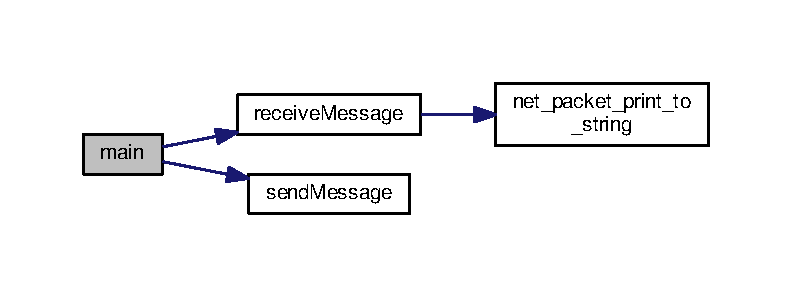
\includegraphics[width=350pt]{load_8cpp_a0ddf1224851353fc92bfbff6f499fa97_cgraph}
\end{center}
\end{figure}


\hypertarget{load_8cpp_a3648412ef7ef48b734fad6e3be1ff5c0}{\index{load.\-cpp@{load.\-cpp}!net\-\_\-packet\-\_\-print\-\_\-to\-\_\-string@{net\-\_\-packet\-\_\-print\-\_\-to\-\_\-string}}
\index{net\-\_\-packet\-\_\-print\-\_\-to\-\_\-string@{net\-\_\-packet\-\_\-print\-\_\-to\-\_\-string}!load.cpp@{load.\-cpp}}
\subsubsection[{net\-\_\-packet\-\_\-print\-\_\-to\-\_\-string}]{\setlength{\rightskip}{0pt plus 5cm}static int net\-\_\-packet\-\_\-print\-\_\-to\-\_\-string (
\begin{DoxyParamCaption}
\item[{const void $\ast$}]{buffer, }
\item[{size\-\_\-t}]{size, }
\item[{void $\ast$}]{packet\-Str}
\end{DoxyParamCaption}
)\hspace{0.3cm}{\ttfamily [static]}}}\label{load_8cpp_a3648412ef7ef48b734fad6e3be1ff5c0}

\begin{DoxyCode}
64 \{
65     \textcolor{keywordtype}{string} *tmpString = (\textcolor{keywordtype}{string} *)packetStr;
66     *tmpString += string((\textcolor{keyword}{const} \textcolor{keywordtype}{char} *)buffer, size);
67     \textcolor{keywordflow}{return} 0;
68 \}
\end{DoxyCode}


이 함수를 호출하는 함수들에 대한 그래프입니다.\-:
\nopagebreak
\begin{figure}[H]
\begin{center}
\leavevmode
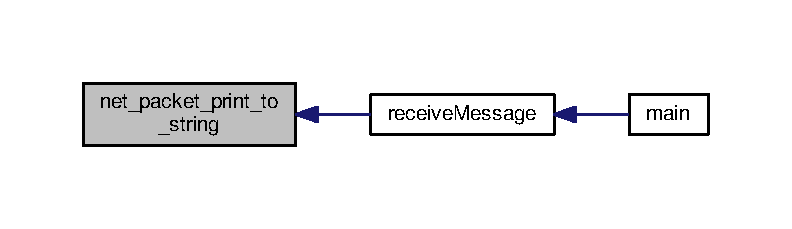
\includegraphics[width=350pt]{load_8cpp_a3648412ef7ef48b734fad6e3be1ff5c0_icgraph}
\end{center}
\end{figure}


\hypertarget{load_8cpp_ab7e9bb8e3de485508865004717ac33cd}{\index{load.\-cpp@{load.\-cpp}!receive\-Message@{receive\-Message}}
\index{receive\-Message@{receive\-Message}!load.cpp@{load.\-cpp}}
\subsubsection[{receive\-Message}]{\setlength{\rightskip}{0pt plus 5cm}Poker\-T\-H\-Message\-\_\-t$\ast$ receive\-Message (
\begin{DoxyParamCaption}
\item[{{\bf Net\-Session} $\ast$}]{session}
\end{DoxyParamCaption}
)}}\label{load_8cpp_ab7e9bb8e3de485508865004717ac33cd}

\begin{DoxyCode}
76 \{
77     PokerTHMessage\_t *msg = NULL;
78     \textcolor{keywordflow}{do} \{
79         asn\_dec\_rval\_t retVal = ber\_decode(0, &asn\_DEF\_PokerTHMessage, (\textcolor{keywordtype}{void} **)&msg, session->
      \hyperlink{struct_net_session_ae53e0baac8f14adba2d5b7d71c715ce7}{recBuf}.data(), session->\hyperlink{struct_net_session_abf9c78874e44c3aa6176e288e77f5aae}{recBufPos});
80         \textcolor{keywordflow}{if}(retVal.code == RC\_OK && msg != NULL) \{
81             \textcolor{keywordflow}{if} (retVal.consumed < session->\hyperlink{struct_net_session_abf9c78874e44c3aa6176e288e77f5aae}{recBufPos}) \{
82                 session->\hyperlink{struct_net_session_abf9c78874e44c3aa6176e288e77f5aae}{recBufPos} -= retVal.consumed;
83                 memmove(session->\hyperlink{struct_net_session_ae53e0baac8f14adba2d5b7d71c715ce7}{recBuf}.c\_array(), session->\hyperlink{struct_net_session_ae53e0baac8f14adba2d5b7d71c715ce7}{recBuf}.c\_array() + retVal.consumed,
       session->\hyperlink{struct_net_session_abf9c78874e44c3aa6176e288e77f5aae}{recBufPos});
84             \} \textcolor{keywordflow}{else} \{
85                 session->\hyperlink{struct_net_session_abf9c78874e44c3aa6176e288e77f5aae}{recBufPos} = 0;
86             \}
87             \textcolor{keywordflow}{if} (asn\_check\_constraints(&asn\_DEF\_PokerTHMessage, msg, NULL, NULL) != 0) \{
88                 cerr << \textcolor{stringliteral}{"Invalid packet received:"} << endl;
89                 \textcolor{keywordtype}{string} packetString;
90                 xer\_encode(&asn\_DEF\_PokerTHMessage, msg, XER\_F\_BASIC, &
      \hyperlink{load_8cpp_a3648412ef7ef48b734fad6e3be1ff5c0}{net\_packet\_print\_to\_string}, &packetString);
91                 cout << packetString << endl;
92             \}
93         \} \textcolor{keywordflow}{else} \{
94             \textcolor{comment}{// Free the partially decoded message (if applicable).}
95             ASN\_STRUCT\_FREE(asn\_DEF\_PokerTHMessage, msg);
96             msg = NULL;
97             session->\hyperlink{struct_net_session_abf9c78874e44c3aa6176e288e77f5aae}{recBufPos} += session->\hyperlink{struct_net_session_a93ead5e6efef575fd61ed0514100310b}{socket}.receive(boost::asio::buffer(session->
      \hyperlink{struct_net_session_ae53e0baac8f14adba2d5b7d71c715ce7}{recBuf}.c\_array() + session->\hyperlink{struct_net_session_abf9c78874e44c3aa6176e288e77f5aae}{recBufPos}, \hyperlink{load_8cpp_a6821bafc3c88dfb2e433a095df9940c6}{BUF\_SIZE} - session->
      \hyperlink{struct_net_session_abf9c78874e44c3aa6176e288e77f5aae}{recBufPos}));
98         \}
99     \} \textcolor{keywordflow}{while} (msg == NULL);
100     \textcolor{keywordflow}{return} msg;
101 \}
\end{DoxyCode}


이 함수 내부에서 호출하는 함수들에 대한 그래프입니다.\-:
\nopagebreak
\begin{figure}[H]
\begin{center}
\leavevmode
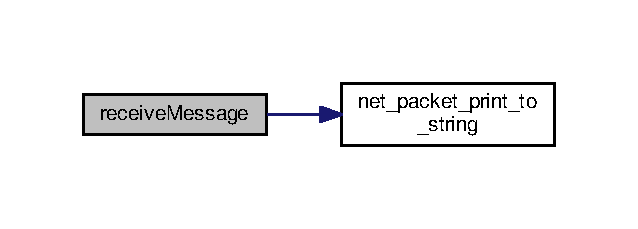
\includegraphics[width=306pt]{load_8cpp_ab7e9bb8e3de485508865004717ac33cd_cgraph}
\end{center}
\end{figure}




이 함수를 호출하는 함수들에 대한 그래프입니다.\-:\nopagebreak
\begin{figure}[H]
\begin{center}
\leavevmode
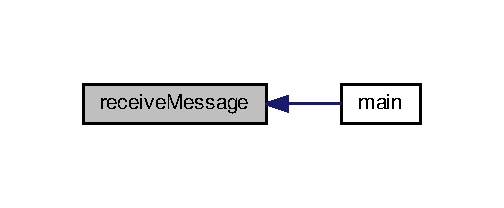
\includegraphics[width=242pt]{load_8cpp_ab7e9bb8e3de485508865004717ac33cd_icgraph}
\end{center}
\end{figure}


\hypertarget{load_8cpp_a147f7872930fe5e0da14572d9bf42100}{\index{load.\-cpp@{load.\-cpp}!send\-Message@{send\-Message}}
\index{send\-Message@{send\-Message}!load.cpp@{load.\-cpp}}
\subsubsection[{send\-Message}]{\setlength{\rightskip}{0pt plus 5cm}bool send\-Message (
\begin{DoxyParamCaption}
\item[{{\bf Net\-Session} $\ast$}]{session, }
\item[{Poker\-T\-H\-Message\-\_\-t $\ast$}]{msg}
\end{DoxyParamCaption}
)}}\label{load_8cpp_a147f7872930fe5e0da14572d9bf42100}

\begin{DoxyCode}
105 \{
106     \textcolor{keywordtype}{bool} retVal = \textcolor{keyword}{false};
107     \textcolor{keywordflow}{if} (msg) \{
108         asn\_enc\_rval\_t e = der\_encode\_to\_buffer(&asn\_DEF\_PokerTHMessage, msg, session->
      \hyperlink{struct_net_session_a6e3c17623ebe78851968a210e95fcc38}{sendBuf}.data(), \hyperlink{load_8cpp_a6821bafc3c88dfb2e433a095df9940c6}{BUF\_SIZE});
109         \textcolor{keywordflow}{if} (e.encoded != -1) \{
110             session->\hyperlink{struct_net_session_a93ead5e6efef575fd61ed0514100310b}{socket}.send(boost::asio::buffer(session->\hyperlink{struct_net_session_a6e3c17623ebe78851968a210e95fcc38}{sendBuf}.data(), e.encoded));
111             retVal = \textcolor{keyword}{true};
112         \}
113         ASN\_STRUCT\_FREE(asn\_DEF\_PokerTHMessage, msg);
114     \}
115     \textcolor{keywordflow}{return} retVal;
116 \}
\end{DoxyCode}


이 함수를 호출하는 함수들에 대한 그래프입니다.\-:\nopagebreak
\begin{figure}[H]
\begin{center}
\leavevmode
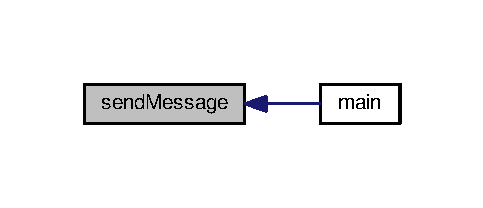
\includegraphics[width=232pt]{load_8cpp_a147f7872930fe5e0da14572d9bf42100_icgraph}
\end{center}
\end{figure}



\hypertarget{pch__game_8h}{\section{pch\-\_\-game.\-h 파일 참조}
\label{pch__game_8h}\index{pch\-\_\-game.\-h@{pch\-\_\-game.\-h}}
}
{\ttfamily \#include \char`\"{}pch\-\_\-lib.\-h\char`\"{}}\\*
pch\-\_\-game.\-h에 대한 include 의존 그래프\nopagebreak
\begin{figure}[H]
\begin{center}
\leavevmode
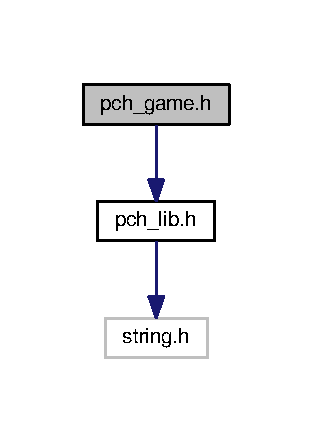
\includegraphics[width=150pt]{pch__game_8h__incl}
\end{center}
\end{figure}

\hypertarget{pch__lib_8h}{\section{pch\-\_\-lib.\-h 파일 참조}
\label{pch__lib_8h}\index{pch\-\_\-lib.\-h@{pch\-\_\-lib.\-h}}
}
{\ttfamily \#include $<$string.\-h$>$}\\*
pch\-\_\-lib.\-h에 대한 include 의존 그래프\nopagebreak
\begin{figure}[H]
\begin{center}
\leavevmode
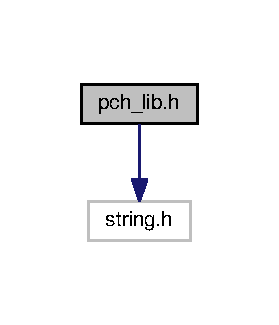
\includegraphics[width=134pt]{pch__lib_8h__incl}
\end{center}
\end{figure}
이 그래프는 이 파일을 직/간접적으로 include 하는 파일들을 보여줍니다.\-:\nopagebreak
\begin{figure}[H]
\begin{center}
\leavevmode
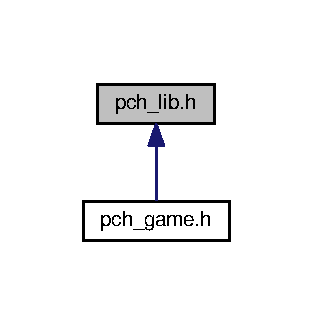
\includegraphics[width=150pt]{pch__lib_8h__dep__incl}
\end{center}
\end{figure}

\hypertarget{playerdata_8cpp}{\section{playerdata.\-cpp 파일 참조}
\label{playerdata_8cpp}\index{playerdata.\-cpp@{playerdata.\-cpp}}
}
{\ttfamily \#include $<$playerdata.\-h$>$}\\*
playerdata.\-cpp에 대한 include 의존 그래프\nopagebreak
\begin{figure}[H]
\begin{center}
\leavevmode
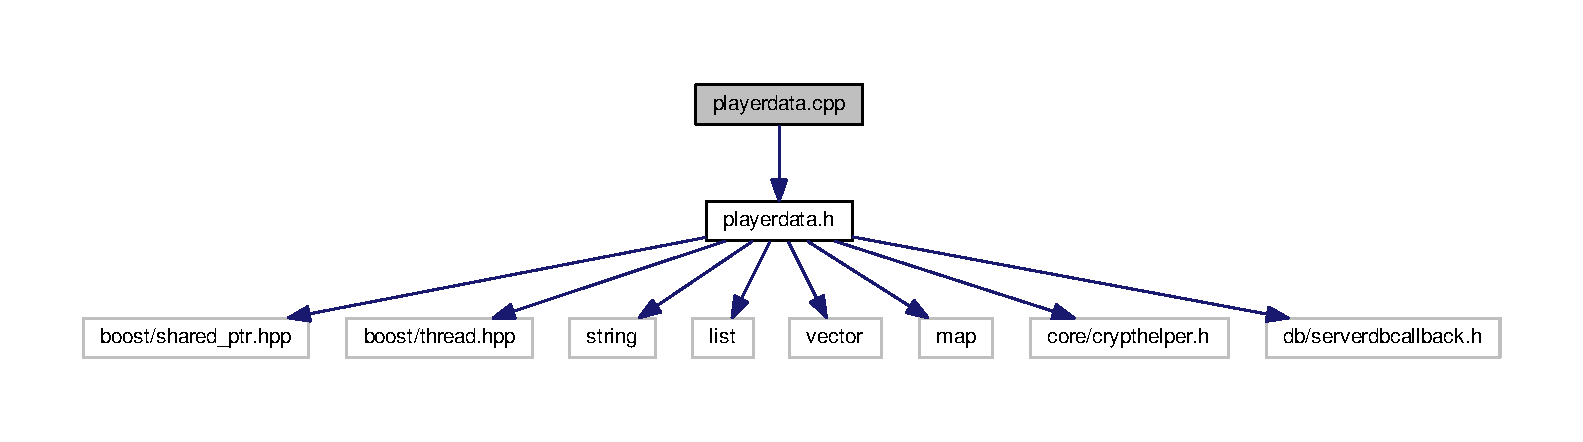
\includegraphics[width=350pt]{playerdata_8cpp__incl}
\end{center}
\end{figure}

\hypertarget{playerdata_8h}{\section{playerdata.\-h 파일 참조}
\label{playerdata_8h}\index{playerdata.\-h@{playerdata.\-h}}
}
{\ttfamily \#include $<$boost/shared\-\_\-ptr.\-hpp$>$}\\*
{\ttfamily \#include $<$boost/thread.\-hpp$>$}\\*
{\ttfamily \#include $<$string$>$}\\*
{\ttfamily \#include $<$list$>$}\\*
{\ttfamily \#include $<$vector$>$}\\*
{\ttfamily \#include $<$map$>$}\\*
{\ttfamily \#include $<$core/crypthelper.\-h$>$}\\*
{\ttfamily \#include $<$db/serverdbcallback.\-h$>$}\\*
playerdata.\-h에 대한 include 의존 그래프\nopagebreak
\begin{figure}[H]
\begin{center}
\leavevmode
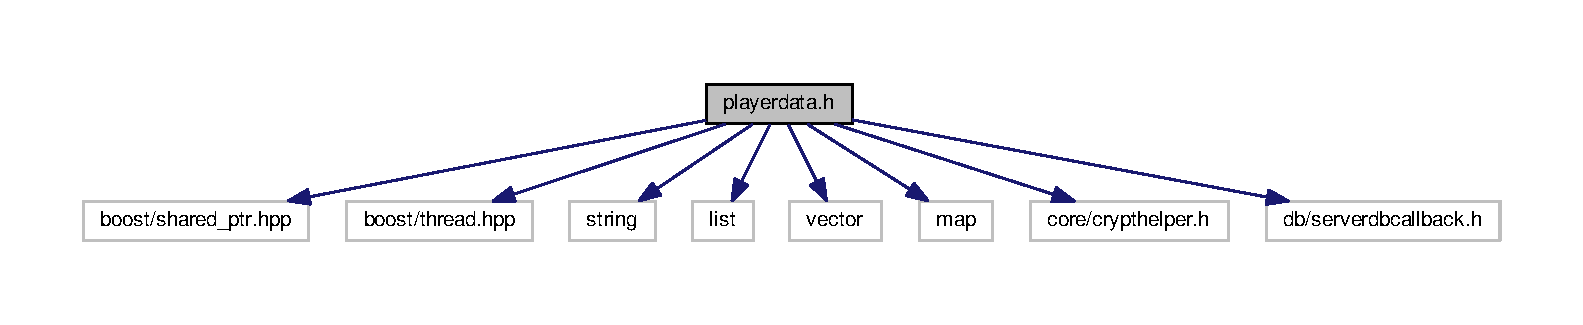
\includegraphics[width=350pt]{playerdata_8h__incl}
\end{center}
\end{figure}
이 그래프는 이 파일을 직/간접적으로 include 하는 파일들을 보여줍니다.\-:\nopagebreak
\begin{figure}[H]
\begin{center}
\leavevmode
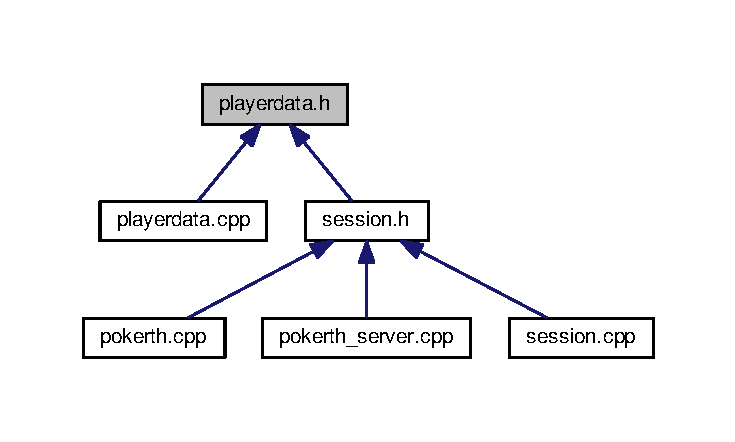
\includegraphics[width=350pt]{playerdata_8h__dep__incl}
\end{center}
\end{figure}
\subsection*{클래스}
\begin{DoxyCompactItemize}
\item 
struct \hyperlink{struct_avatar_file}{Avatar\-File}
\item 
struct \hyperlink{struct_player_info}{Player\-Info}
\item 
class \hyperlink{class_player_data}{Player\-Data}
\end{DoxyCompactItemize}
\subsection*{타입정의}
\begin{DoxyCompactItemize}
\item 
typedef std\-::list$<$ std\-::pair\\*
$<$ unsigned, unsigned $>$ $>$ \hyperlink{playerdata_8h_a5423ca985c99b02536f56d0384628905}{Remove\-Player\-List}
\item 
typedef std\-::list\\*
$<$ boost\-::shared\-\_\-ptr\\*
$<$ \hyperlink{class_player_data}{Player\-Data} $>$ $>$ \hyperlink{playerdata_8h_a8232751bca13b3cf3056ce08251f7067}{Player\-Data\-List}
\item 
typedef std\-::map$<$ unsigned, \\*
boost\-::shared\-\_\-ptr$<$ \hyperlink{class_player_data}{Player\-Data} $>$ $>$ \hyperlink{playerdata_8h_a9e3683fd7e0a765d8420195eec7abcf2}{Player\-Data\-Map}
\end{DoxyCompactItemize}
\subsection*{열거형 타입}
\begin{DoxyCompactItemize}
\item 
enum \hyperlink{playerdata_8h_abe590f3c9109f404f003d5d7e4f0fccf}{Player\-Type} \{ \hyperlink{playerdata_8h_abe590f3c9109f404f003d5d7e4f0fccfaafb128e5bf75c3d00a6de25a025f61d6}{P\-L\-A\-Y\-E\-R\-\_\-\-T\-Y\-P\-E\-\_\-\-C\-O\-M\-P\-U\-T\-E\-R}, 
\hyperlink{playerdata_8h_abe590f3c9109f404f003d5d7e4f0fccfa6bf6033830c666c7491c430f7ff395a0}{P\-L\-A\-Y\-E\-R\-\_\-\-T\-Y\-P\-E\-\_\-\-H\-U\-M\-A\-N}
 \}
\item 
enum \hyperlink{playerdata_8h_ac0c72aca5c5ceabb2abbcd2d2c02aba6}{Player\-Rights} \{ \hyperlink{playerdata_8h_ac0c72aca5c5ceabb2abbcd2d2c02aba6a32d17691c0f17eb117f004b3fdd90685}{P\-L\-A\-Y\-E\-R\-\_\-\-R\-I\-G\-H\-T\-S\-\_\-\-G\-U\-E\-S\-T} = 1, 
\hyperlink{playerdata_8h_ac0c72aca5c5ceabb2abbcd2d2c02aba6a716d25099e5fdf1bad19d51f79bbd7ab}{P\-L\-A\-Y\-E\-R\-\_\-\-R\-I\-G\-H\-T\-S\-\_\-\-N\-O\-R\-M\-A\-L}, 
\hyperlink{playerdata_8h_ac0c72aca5c5ceabb2abbcd2d2c02aba6aad750e9e1dec0aa30d5ad3bcaa4bb9ad}{P\-L\-A\-Y\-E\-R\-\_\-\-R\-I\-G\-H\-T\-S\-\_\-\-A\-D\-M\-I\-N}
 \}
\item 
enum \hyperlink{playerdata_8h_a838468e0dd027767b891761d30d2bf39}{Avatar\-File\-Type} \{ \hyperlink{playerdata_8h_a838468e0dd027767b891761d30d2bf39af3195e1aaeb82da02f85ea7a293e91a1}{A\-V\-A\-T\-A\-R\-\_\-\-F\-I\-L\-E\-\_\-\-T\-Y\-P\-E\-\_\-\-U\-N\-K\-N\-O\-W\-N} = 0, 
\hyperlink{playerdata_8h_a838468e0dd027767b891761d30d2bf39ae549f363f4e70692202d4cec6c67622a}{A\-V\-A\-T\-A\-R\-\_\-\-F\-I\-L\-E\-\_\-\-T\-Y\-P\-E\-\_\-\-P\-N\-G}, 
\hyperlink{playerdata_8h_a838468e0dd027767b891761d30d2bf39a27c2a1d992cddf30f80ccd24f73bfda6}{A\-V\-A\-T\-A\-R\-\_\-\-F\-I\-L\-E\-\_\-\-T\-Y\-P\-E\-\_\-\-J\-P\-G}, 
\hyperlink{playerdata_8h_a838468e0dd027767b891761d30d2bf39a9e74053704295efe86723ba5f522448f}{A\-V\-A\-T\-A\-R\-\_\-\-F\-I\-L\-E\-\_\-\-T\-Y\-P\-E\-\_\-\-G\-I\-F}
 \}
\end{DoxyCompactItemize}


\subsection{타입정의 문서화}
\hypertarget{playerdata_8h_a8232751bca13b3cf3056ce08251f7067}{\index{playerdata.\-h@{playerdata.\-h}!Player\-Data\-List@{Player\-Data\-List}}
\index{Player\-Data\-List@{Player\-Data\-List}!playerdata.h@{playerdata.\-h}}
\subsubsection[{Player\-Data\-List}]{\setlength{\rightskip}{0pt plus 5cm}typedef std\-::list$<$boost\-::shared\-\_\-ptr$<${\bf Player\-Data}$>$ $>$ {\bf Player\-Data\-List}}}\label{playerdata_8h_a8232751bca13b3cf3056ce08251f7067}
\hypertarget{playerdata_8h_a9e3683fd7e0a765d8420195eec7abcf2}{\index{playerdata.\-h@{playerdata.\-h}!Player\-Data\-Map@{Player\-Data\-Map}}
\index{Player\-Data\-Map@{Player\-Data\-Map}!playerdata.h@{playerdata.\-h}}
\subsubsection[{Player\-Data\-Map}]{\setlength{\rightskip}{0pt plus 5cm}typedef std\-::map$<$unsigned, boost\-::shared\-\_\-ptr$<${\bf Player\-Data}$>$ $>$ {\bf Player\-Data\-Map}}}\label{playerdata_8h_a9e3683fd7e0a765d8420195eec7abcf2}
\hypertarget{playerdata_8h_a5423ca985c99b02536f56d0384628905}{\index{playerdata.\-h@{playerdata.\-h}!Remove\-Player\-List@{Remove\-Player\-List}}
\index{Remove\-Player\-List@{Remove\-Player\-List}!playerdata.h@{playerdata.\-h}}
\subsubsection[{Remove\-Player\-List}]{\setlength{\rightskip}{0pt plus 5cm}typedef std\-::list$<$std\-::pair$<$unsigned, unsigned$>$ $>$ {\bf Remove\-Player\-List}}}\label{playerdata_8h_a5423ca985c99b02536f56d0384628905}


\subsection{열거형 타입 문서화}
\hypertarget{playerdata_8h_a838468e0dd027767b891761d30d2bf39}{\index{playerdata.\-h@{playerdata.\-h}!Avatar\-File\-Type@{Avatar\-File\-Type}}
\index{Avatar\-File\-Type@{Avatar\-File\-Type}!playerdata.h@{playerdata.\-h}}
\subsubsection[{Avatar\-File\-Type}]{\setlength{\rightskip}{0pt plus 5cm}enum {\bf Avatar\-File\-Type}}}\label{playerdata_8h_a838468e0dd027767b891761d30d2bf39}
\begin{Desc}
\item[열거형 멤버]\par
\begin{description}
\index{A\-V\-A\-T\-A\-R\-\_\-\-F\-I\-L\-E\-\_\-\-T\-Y\-P\-E\-\_\-\-U\-N\-K\-N\-O\-W\-N@{A\-V\-A\-T\-A\-R\-\_\-\-F\-I\-L\-E\-\_\-\-T\-Y\-P\-E\-\_\-\-U\-N\-K\-N\-O\-W\-N}!playerdata.\-h@{playerdata.\-h}}\index{playerdata.\-h@{playerdata.\-h}!A\-V\-A\-T\-A\-R\-\_\-\-F\-I\-L\-E\-\_\-\-T\-Y\-P\-E\-\_\-\-U\-N\-K\-N\-O\-W\-N@{A\-V\-A\-T\-A\-R\-\_\-\-F\-I\-L\-E\-\_\-\-T\-Y\-P\-E\-\_\-\-U\-N\-K\-N\-O\-W\-N}}\item[{\em 
\hypertarget{playerdata_8h_a838468e0dd027767b891761d30d2bf39af3195e1aaeb82da02f85ea7a293e91a1}{A\-V\-A\-T\-A\-R\-\_\-\-F\-I\-L\-E\-\_\-\-T\-Y\-P\-E\-\_\-\-U\-N\-K\-N\-O\-W\-N}\label{playerdata_8h_a838468e0dd027767b891761d30d2bf39af3195e1aaeb82da02f85ea7a293e91a1}
}]\index{A\-V\-A\-T\-A\-R\-\_\-\-F\-I\-L\-E\-\_\-\-T\-Y\-P\-E\-\_\-\-P\-N\-G@{A\-V\-A\-T\-A\-R\-\_\-\-F\-I\-L\-E\-\_\-\-T\-Y\-P\-E\-\_\-\-P\-N\-G}!playerdata.\-h@{playerdata.\-h}}\index{playerdata.\-h@{playerdata.\-h}!A\-V\-A\-T\-A\-R\-\_\-\-F\-I\-L\-E\-\_\-\-T\-Y\-P\-E\-\_\-\-P\-N\-G@{A\-V\-A\-T\-A\-R\-\_\-\-F\-I\-L\-E\-\_\-\-T\-Y\-P\-E\-\_\-\-P\-N\-G}}\item[{\em 
\hypertarget{playerdata_8h_a838468e0dd027767b891761d30d2bf39ae549f363f4e70692202d4cec6c67622a}{A\-V\-A\-T\-A\-R\-\_\-\-F\-I\-L\-E\-\_\-\-T\-Y\-P\-E\-\_\-\-P\-N\-G}\label{playerdata_8h_a838468e0dd027767b891761d30d2bf39ae549f363f4e70692202d4cec6c67622a}
}]\index{A\-V\-A\-T\-A\-R\-\_\-\-F\-I\-L\-E\-\_\-\-T\-Y\-P\-E\-\_\-\-J\-P\-G@{A\-V\-A\-T\-A\-R\-\_\-\-F\-I\-L\-E\-\_\-\-T\-Y\-P\-E\-\_\-\-J\-P\-G}!playerdata.\-h@{playerdata.\-h}}\index{playerdata.\-h@{playerdata.\-h}!A\-V\-A\-T\-A\-R\-\_\-\-F\-I\-L\-E\-\_\-\-T\-Y\-P\-E\-\_\-\-J\-P\-G@{A\-V\-A\-T\-A\-R\-\_\-\-F\-I\-L\-E\-\_\-\-T\-Y\-P\-E\-\_\-\-J\-P\-G}}\item[{\em 
\hypertarget{playerdata_8h_a838468e0dd027767b891761d30d2bf39a27c2a1d992cddf30f80ccd24f73bfda6}{A\-V\-A\-T\-A\-R\-\_\-\-F\-I\-L\-E\-\_\-\-T\-Y\-P\-E\-\_\-\-J\-P\-G}\label{playerdata_8h_a838468e0dd027767b891761d30d2bf39a27c2a1d992cddf30f80ccd24f73bfda6}
}]\index{A\-V\-A\-T\-A\-R\-\_\-\-F\-I\-L\-E\-\_\-\-T\-Y\-P\-E\-\_\-\-G\-I\-F@{A\-V\-A\-T\-A\-R\-\_\-\-F\-I\-L\-E\-\_\-\-T\-Y\-P\-E\-\_\-\-G\-I\-F}!playerdata.\-h@{playerdata.\-h}}\index{playerdata.\-h@{playerdata.\-h}!A\-V\-A\-T\-A\-R\-\_\-\-F\-I\-L\-E\-\_\-\-T\-Y\-P\-E\-\_\-\-G\-I\-F@{A\-V\-A\-T\-A\-R\-\_\-\-F\-I\-L\-E\-\_\-\-T\-Y\-P\-E\-\_\-\-G\-I\-F}}\item[{\em 
\hypertarget{playerdata_8h_a838468e0dd027767b891761d30d2bf39a9e74053704295efe86723ba5f522448f}{A\-V\-A\-T\-A\-R\-\_\-\-F\-I\-L\-E\-\_\-\-T\-Y\-P\-E\-\_\-\-G\-I\-F}\label{playerdata_8h_a838468e0dd027767b891761d30d2bf39a9e74053704295efe86723ba5f522448f}
}]\end{description}
\end{Desc}

\begin{DoxyCode}
58                     \{
59     \hyperlink{playerdata_8h_a838468e0dd027767b891761d30d2bf39af3195e1aaeb82da02f85ea7a293e91a1}{AVATAR\_FILE\_TYPE\_UNKNOWN} = 0,
60     \hyperlink{playerdata_8h_a838468e0dd027767b891761d30d2bf39ae549f363f4e70692202d4cec6c67622a}{AVATAR\_FILE\_TYPE\_PNG},
61     \hyperlink{playerdata_8h_a838468e0dd027767b891761d30d2bf39a27c2a1d992cddf30f80ccd24f73bfda6}{AVATAR\_FILE\_TYPE\_JPG},
62     \hyperlink{playerdata_8h_a838468e0dd027767b891761d30d2bf39a9e74053704295efe86723ba5f522448f}{AVATAR\_FILE\_TYPE\_GIF}
63 \};
\end{DoxyCode}
\hypertarget{playerdata_8h_ac0c72aca5c5ceabb2abbcd2d2c02aba6}{\index{playerdata.\-h@{playerdata.\-h}!Player\-Rights@{Player\-Rights}}
\index{Player\-Rights@{Player\-Rights}!playerdata.h@{playerdata.\-h}}
\subsubsection[{Player\-Rights}]{\setlength{\rightskip}{0pt plus 5cm}enum {\bf Player\-Rights}}}\label{playerdata_8h_ac0c72aca5c5ceabb2abbcd2d2c02aba6}
\begin{Desc}
\item[열거형 멤버]\par
\begin{description}
\index{P\-L\-A\-Y\-E\-R\-\_\-\-R\-I\-G\-H\-T\-S\-\_\-\-G\-U\-E\-S\-T@{P\-L\-A\-Y\-E\-R\-\_\-\-R\-I\-G\-H\-T\-S\-\_\-\-G\-U\-E\-S\-T}!playerdata.\-h@{playerdata.\-h}}\index{playerdata.\-h@{playerdata.\-h}!P\-L\-A\-Y\-E\-R\-\_\-\-R\-I\-G\-H\-T\-S\-\_\-\-G\-U\-E\-S\-T@{P\-L\-A\-Y\-E\-R\-\_\-\-R\-I\-G\-H\-T\-S\-\_\-\-G\-U\-E\-S\-T}}\item[{\em 
\hypertarget{playerdata_8h_ac0c72aca5c5ceabb2abbcd2d2c02aba6a32d17691c0f17eb117f004b3fdd90685}{P\-L\-A\-Y\-E\-R\-\_\-\-R\-I\-G\-H\-T\-S\-\_\-\-G\-U\-E\-S\-T}\label{playerdata_8h_ac0c72aca5c5ceabb2abbcd2d2c02aba6a32d17691c0f17eb117f004b3fdd90685}
}]\index{P\-L\-A\-Y\-E\-R\-\_\-\-R\-I\-G\-H\-T\-S\-\_\-\-N\-O\-R\-M\-A\-L@{P\-L\-A\-Y\-E\-R\-\_\-\-R\-I\-G\-H\-T\-S\-\_\-\-N\-O\-R\-M\-A\-L}!playerdata.\-h@{playerdata.\-h}}\index{playerdata.\-h@{playerdata.\-h}!P\-L\-A\-Y\-E\-R\-\_\-\-R\-I\-G\-H\-T\-S\-\_\-\-N\-O\-R\-M\-A\-L@{P\-L\-A\-Y\-E\-R\-\_\-\-R\-I\-G\-H\-T\-S\-\_\-\-N\-O\-R\-M\-A\-L}}\item[{\em 
\hypertarget{playerdata_8h_ac0c72aca5c5ceabb2abbcd2d2c02aba6a716d25099e5fdf1bad19d51f79bbd7ab}{P\-L\-A\-Y\-E\-R\-\_\-\-R\-I\-G\-H\-T\-S\-\_\-\-N\-O\-R\-M\-A\-L}\label{playerdata_8h_ac0c72aca5c5ceabb2abbcd2d2c02aba6a716d25099e5fdf1bad19d51f79bbd7ab}
}]\index{P\-L\-A\-Y\-E\-R\-\_\-\-R\-I\-G\-H\-T\-S\-\_\-\-A\-D\-M\-I\-N@{P\-L\-A\-Y\-E\-R\-\_\-\-R\-I\-G\-H\-T\-S\-\_\-\-A\-D\-M\-I\-N}!playerdata.\-h@{playerdata.\-h}}\index{playerdata.\-h@{playerdata.\-h}!P\-L\-A\-Y\-E\-R\-\_\-\-R\-I\-G\-H\-T\-S\-\_\-\-A\-D\-M\-I\-N@{P\-L\-A\-Y\-E\-R\-\_\-\-R\-I\-G\-H\-T\-S\-\_\-\-A\-D\-M\-I\-N}}\item[{\em 
\hypertarget{playerdata_8h_ac0c72aca5c5ceabb2abbcd2d2c02aba6aad750e9e1dec0aa30d5ad3bcaa4bb9ad}{P\-L\-A\-Y\-E\-R\-\_\-\-R\-I\-G\-H\-T\-S\-\_\-\-A\-D\-M\-I\-N}\label{playerdata_8h_ac0c72aca5c5ceabb2abbcd2d2c02aba6aad750e9e1dec0aa30d5ad3bcaa4bb9ad}
}]\end{description}
\end{Desc}

\begin{DoxyCode}
52                   \{
53     \hyperlink{playerdata_8h_ac0c72aca5c5ceabb2abbcd2d2c02aba6a32d17691c0f17eb117f004b3fdd90685}{PLAYER\_RIGHTS\_GUEST} = 1,
54     \hyperlink{playerdata_8h_ac0c72aca5c5ceabb2abbcd2d2c02aba6a716d25099e5fdf1bad19d51f79bbd7ab}{PLAYER\_RIGHTS\_NORMAL},
55     \hyperlink{playerdata_8h_ac0c72aca5c5ceabb2abbcd2d2c02aba6aad750e9e1dec0aa30d5ad3bcaa4bb9ad}{PLAYER\_RIGHTS\_ADMIN}
56 \};
\end{DoxyCode}
\hypertarget{playerdata_8h_abe590f3c9109f404f003d5d7e4f0fccf}{\index{playerdata.\-h@{playerdata.\-h}!Player\-Type@{Player\-Type}}
\index{Player\-Type@{Player\-Type}!playerdata.h@{playerdata.\-h}}
\subsubsection[{Player\-Type}]{\setlength{\rightskip}{0pt plus 5cm}enum {\bf Player\-Type}}}\label{playerdata_8h_abe590f3c9109f404f003d5d7e4f0fccf}
\begin{Desc}
\item[열거형 멤버]\par
\begin{description}
\index{P\-L\-A\-Y\-E\-R\-\_\-\-T\-Y\-P\-E\-\_\-\-C\-O\-M\-P\-U\-T\-E\-R@{P\-L\-A\-Y\-E\-R\-\_\-\-T\-Y\-P\-E\-\_\-\-C\-O\-M\-P\-U\-T\-E\-R}!playerdata.\-h@{playerdata.\-h}}\index{playerdata.\-h@{playerdata.\-h}!P\-L\-A\-Y\-E\-R\-\_\-\-T\-Y\-P\-E\-\_\-\-C\-O\-M\-P\-U\-T\-E\-R@{P\-L\-A\-Y\-E\-R\-\_\-\-T\-Y\-P\-E\-\_\-\-C\-O\-M\-P\-U\-T\-E\-R}}\item[{\em 
\hypertarget{playerdata_8h_abe590f3c9109f404f003d5d7e4f0fccfaafb128e5bf75c3d00a6de25a025f61d6}{P\-L\-A\-Y\-E\-R\-\_\-\-T\-Y\-P\-E\-\_\-\-C\-O\-M\-P\-U\-T\-E\-R}\label{playerdata_8h_abe590f3c9109f404f003d5d7e4f0fccfaafb128e5bf75c3d00a6de25a025f61d6}
}]\index{P\-L\-A\-Y\-E\-R\-\_\-\-T\-Y\-P\-E\-\_\-\-H\-U\-M\-A\-N@{P\-L\-A\-Y\-E\-R\-\_\-\-T\-Y\-P\-E\-\_\-\-H\-U\-M\-A\-N}!playerdata.\-h@{playerdata.\-h}}\index{playerdata.\-h@{playerdata.\-h}!P\-L\-A\-Y\-E\-R\-\_\-\-T\-Y\-P\-E\-\_\-\-H\-U\-M\-A\-N@{P\-L\-A\-Y\-E\-R\-\_\-\-T\-Y\-P\-E\-\_\-\-H\-U\-M\-A\-N}}\item[{\em 
\hypertarget{playerdata_8h_abe590f3c9109f404f003d5d7e4f0fccfa6bf6033830c666c7491c430f7ff395a0}{P\-L\-A\-Y\-E\-R\-\_\-\-T\-Y\-P\-E\-\_\-\-H\-U\-M\-A\-N}\label{playerdata_8h_abe590f3c9109f404f003d5d7e4f0fccfa6bf6033830c666c7491c430f7ff395a0}
}]\end{description}
\end{Desc}

\begin{DoxyCode}
47                 \{
48     \hyperlink{playerdata_8h_abe590f3c9109f404f003d5d7e4f0fccfaafb128e5bf75c3d00a6de25a025f61d6}{PLAYER\_TYPE\_COMPUTER},
49     \hyperlink{playerdata_8h_abe590f3c9109f404f003d5d7e4f0fccfa6bf6033830c666c7491c430f7ff395a0}{PLAYER\_TYPE\_HUMAN}
50 \};
\end{DoxyCode}

\hypertarget{pokerth_8cpp}{\section{pokerth.\-cpp 파일 참조}
\label{pokerth_8cpp}\index{pokerth.\-cpp@{pokerth.\-cpp}}
}
{\ttfamily \#include $<$boost/asio.\-hpp$>$}\\*
{\ttfamily \#include $<$iostream$>$}\\*
{\ttfamily \#include $<$cstdlib$>$}\\*
{\ttfamily \#include $<$ctime$>$}\\*
{\ttfamily \#include $<$qapplication.\-h$>$}\\*
{\ttfamily \#include $<$Qt\-Gui$>$}\\*
{\ttfamily \#include $<$Qt\-Core$>$}\\*
{\ttfamily \#include $<$curl/curl.\-h$>$}\\*
{\ttfamily \#include \char`\"{}session.\-h\char`\"{}}\\*
{\ttfamily \#include \char`\"{}startwindowimpl.\-h\char`\"{}}\\*
{\ttfamily \#include \char`\"{}configfile.\-h\char`\"{}}\\*
{\ttfamily \#include \char`\"{}log.\-h\char`\"{}}\\*
{\ttfamily \#include \char`\"{}startsplash.\-h\char`\"{}}\\*
{\ttfamily \#include \char`\"{}game\-\_\-defs.\-h\char`\"{}}\\*
{\ttfamily \#include $<$net/socket\-\_\-startup.\-h$>$}\\*
{\ttfamily \#include $<$third\-\_\-party/qtsingleapplication/qtsingleapplication.\-h$>$}\\*
pokerth.\-cpp에 대한 include 의존 그래프\nopagebreak
\begin{figure}[H]
\begin{center}
\leavevmode
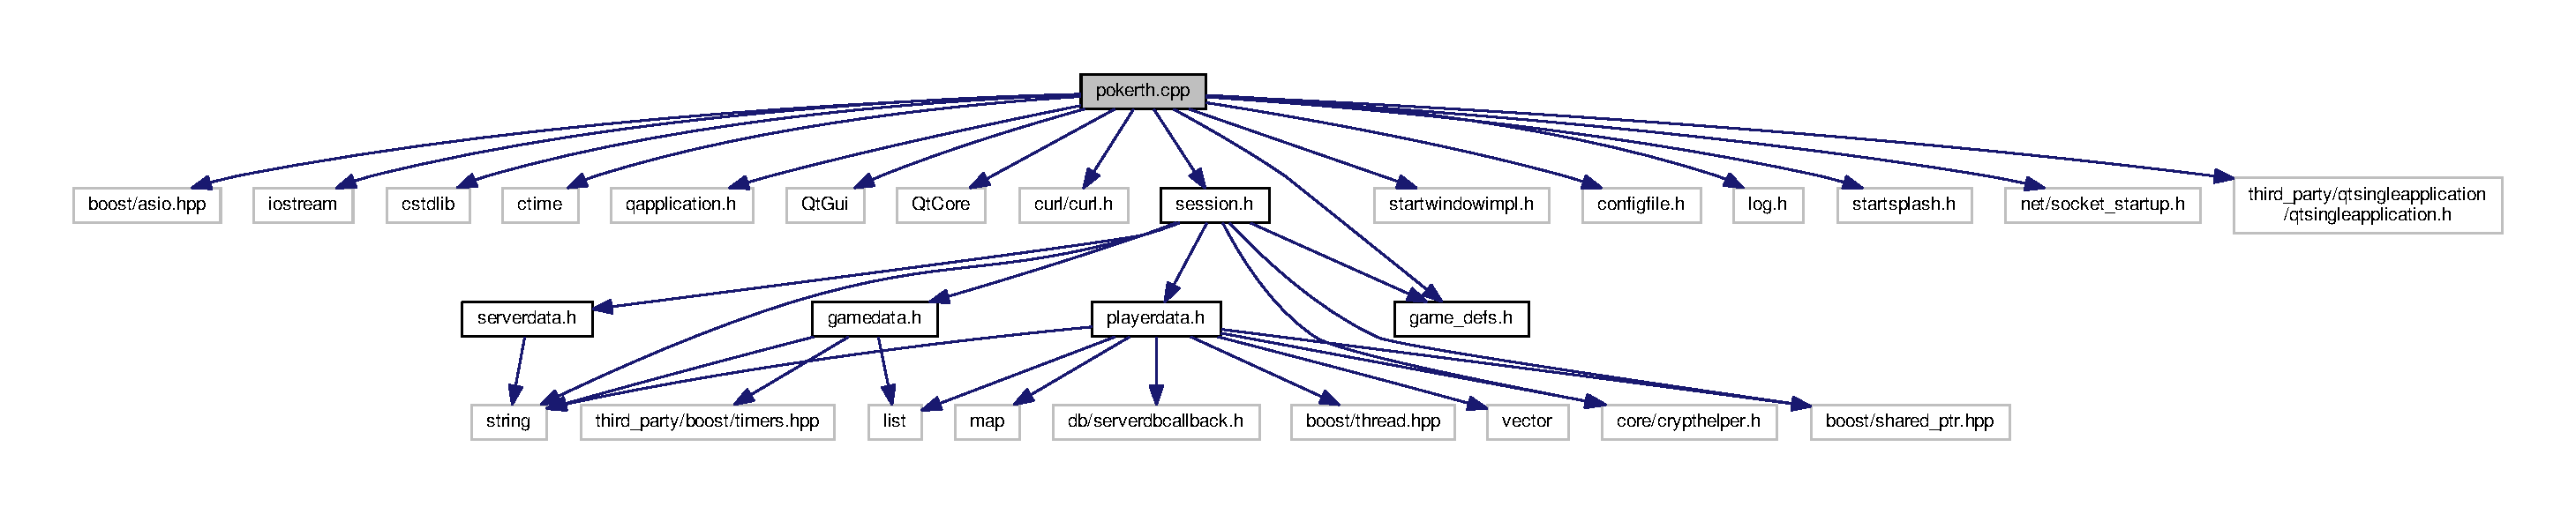
\includegraphics[width=350pt]{pokerth_8cpp__incl}
\end{center}
\end{figure}
\subsection*{매크로}
\begin{DoxyCompactItemize}
\item 
\#define \hyperlink{pokerth_8cpp_a1bdcac39cce77af91b60ca6044fae397}{E\-N\-A\-B\-L\-E\-\_\-\-L\-E\-A\-K\-\_\-\-C\-H\-E\-C\-K}()
\end{DoxyCompactItemize}
\subsection*{함수}
\begin{DoxyCompactItemize}
\item 
int \hyperlink{pokerth_8cpp_a3c04138a5bfe5d72780bb7e82a18e627}{main} (int argc, char $\ast$$\ast$argv)
\end{DoxyCompactItemize}


\subsection{매크로 문서화}
\hypertarget{pokerth_8cpp_a1bdcac39cce77af91b60ca6044fae397}{\index{pokerth.\-cpp@{pokerth.\-cpp}!E\-N\-A\-B\-L\-E\-\_\-\-L\-E\-A\-K\-\_\-\-C\-H\-E\-C\-K@{E\-N\-A\-B\-L\-E\-\_\-\-L\-E\-A\-K\-\_\-\-C\-H\-E\-C\-K}}
\index{E\-N\-A\-B\-L\-E\-\_\-\-L\-E\-A\-K\-\_\-\-C\-H\-E\-C\-K@{E\-N\-A\-B\-L\-E\-\_\-\-L\-E\-A\-K\-\_\-\-C\-H\-E\-C\-K}!pokerth.cpp@{pokerth.\-cpp}}
\subsubsection[{E\-N\-A\-B\-L\-E\-\_\-\-L\-E\-A\-K\-\_\-\-C\-H\-E\-C\-K}]{\setlength{\rightskip}{0pt plus 5cm}\#define E\-N\-A\-B\-L\-E\-\_\-\-L\-E\-A\-K\-\_\-\-C\-H\-E\-C\-K(
\begin{DoxyParamCaption}
{}
\end{DoxyParamCaption}
)}}\label{pokerth_8cpp_a1bdcac39cce77af91b60ca6044fae397}


\subsection{함수 문서화}
\hypertarget{pokerth_8cpp_a3c04138a5bfe5d72780bb7e82a18e627}{\index{pokerth.\-cpp@{pokerth.\-cpp}!main@{main}}
\index{main@{main}!pokerth.cpp@{pokerth.\-cpp}}
\subsubsection[{main}]{\setlength{\rightskip}{0pt plus 5cm}int main (
\begin{DoxyParamCaption}
\item[{int}]{argc, }
\item[{char $\ast$$\ast$}]{argv}
\end{DoxyParamCaption}
)}}\label{pokerth_8cpp_a3c04138a5bfe5d72780bb7e82a18e627}

\begin{DoxyCode}
116 \{
117 
118     \textcolor{comment}{//ENABLE\_LEAK\_CHECK();}
119 
120     \textcolor{comment}{//\_CrtSetBreakAlloc(49937);}
121     socket\_startup();
122     curl\_global\_init(CURL\_GLOBAL\_NOTHING);
123 
124 \textcolor{preprocessor}{#ifdef \_\_APPLE\_\_
}
125 \textcolor{preprocessor}{}    \textcolor{comment}{// The following needs to be done before the application is created, otherwise loading platforms plugin
       fails.}
126     QDir dir(argv[0]);
127     dir.cdUp();
128     dir.cdUp();
129     dir.cd(\textcolor{stringliteral}{"plugins"});
130     QApplication::setLibraryPaths(QStringList(dir.absolutePath()));
131 \textcolor{preprocessor}{#endif
}
132 \textcolor{preprocessor}{}
134 \textcolor{preprocessor}{#ifdef ANDROID
}
135 \textcolor{preprocessor}{}    QApplication a(argc, argv);
136     a.setApplicationName(\textcolor{stringliteral}{"PokerTH"});
137 \textcolor{preprocessor}{#else
}
138 \textcolor{preprocessor}{}    SharedTools::QtSingleApplication a( \textcolor{stringliteral}{"PokerTH"}, argc, argv );
139     \textcolor{keywordflow}{if} (a.sendMessage(\textcolor{stringliteral}{"Wake up!"})) \{
140         \textcolor{keywordflow}{return} 0;
141     \}
142 \textcolor{preprocessor}{#endif
}
143 \textcolor{preprocessor}{}
144     \textcolor{comment}{//create defaultconfig}
145     ConfigFile *myConfig = \textcolor{keyword}{new} ConfigFile(argv[0], \textcolor{keyword}{false});
146     Log *myLog = \textcolor{keyword}{new} Log(myConfig);
147 
148     \textcolor{comment}{// set PlastiqueStyle even for mac-version to prevent artefacts on styled widgets}
149 \textcolor{preprocessor}{#if QT\_VERSION < 0x050000
}
150 \textcolor{preprocessor}{}    a.setStyle(\textcolor{keyword}{new} QPlastiqueStyle);
151 \textcolor{preprocessor}{#endif
}
152 \textcolor{preprocessor}{}
153     QString myAppDataPath = QString::fromUtf8(myConfig->readConfigString(\textcolor{stringliteral}{"AppDataDir"}).c\_str());
154     \textcolor{comment}{//set QApplication default font}
155 
156     QFontDatabase::addApplicationFont (myAppDataPath +\textcolor{stringliteral}{"fonts/n019003l.pfb"});
157     QFontDatabase::addApplicationFont (myAppDataPath +\textcolor{stringliteral}{"fonts/DejaVuSans-Bold.ttf"});
158 
159 \textcolor{preprocessor}{#ifdef \_WIN32
}
160 \textcolor{preprocessor}{}    QString font1String(\textcolor{stringliteral}{"QApplication, QWidget, QDialog \{ font-size: 12px; \}"});
161 \textcolor{preprocessor}{#elif \_\_APPLE\_\_
}
162 \textcolor{preprocessor}{}    \textcolor{comment}{//            QString font1String("font-family: \(\backslash\)"Lucida Grande\(\backslash\)";");}
163     QString font1String(\textcolor{stringliteral}{"QApplication, QWidget, QDialog \{ font-size: 11px; \}"});
164 \textcolor{preprocessor}{#elif ANDROID
}
165 \textcolor{preprocessor}{}    QString font1String(\textcolor{stringliteral}{"QApplication, QWidget, QDialog \{ font-family: \(\backslash\)"Nimbus Sans L\(\backslash\)"; font-size: 26px;
       \}"});
166     QPalette p = a.palette();
167     p.setColor(\hyperlink{game__defs_8h_a03bfec859eac87be20f8952c1eb89de0}{QPalette::Button}, QColor::fromRgb(80,80,80));
168     p.setColor(QPalette::Base, QColor::fromRgb(80,80,80));
169     p.setColor(QPalette::Window, QColor::fromRgb(50,50,50));
170     p.setColor(QPalette::ButtonText, QColor::fromRgb(255,255,255));
171     p.setColor(QPalette::Disabled, QPalette::ButtonText, QColor::fromRgb(130,130,130));
172     p.setColor(QPalette::WindowText, QColor::fromRgb(255,255,255));
173     p.setColor(QPalette::Disabled, QPalette::WindowText, QColor::fromRgb(100,100,100));
174     p.setColor(QPalette::Text, QColor::fromRgb(255,255,255));
175     p.setColor(QPalette::Disabled, QPalette::Text, QColor::fromRgb(100,100,100));
176     p.setColor(QPalette::Link, QColor::fromRgb(192,192,255));
177     p.setColor(QPalette::LinkVisited, QColor::fromRgb(192,192,255));
178     a.setPalette(p);
179 \textcolor{preprocessor}{#elif MAEMO
}
180 \textcolor{preprocessor}{}    QString font1String(\textcolor{stringliteral}{"QApplication, QWidget, QDialog \{ font-family: \(\backslash\)"Nimbus Sans L\(\backslash\)"; font-size: 22px;
       \}"});
181     QPalette p = a.palette();
182     p.setColor(\hyperlink{game__defs_8h_a03bfec859eac87be20f8952c1eb89de0}{QPalette::Button}, QColor::fromRgb(80,80,80));
183     p.setColor(QPalette::Base, QColor::fromRgb(80,80,80));
184     p.setColor(QPalette::Window, QColor::fromRgb(50,50,50));
185     p.setColor(QPalette::ButtonText, QColor::fromRgb(255,255,255));
186     p.setColor(QPalette::Disabled, QPalette::ButtonText, QColor::fromRgb(100,100,100));
187     p.setColor(QPalette::WindowText, QColor::fromRgb(255,255,255));
188     p.setColor(QPalette::Disabled, QPalette::WindowText, QColor::fromRgb(100,100,100));
189     p.setColor(QPalette::Text, QColor::fromRgb(255,255,255));
190     p.setColor(QPalette::Disabled, QPalette::Text, QColor::fromRgb(100,100,100));
191     p.setColor(QPalette::Link, QColor::fromRgb(192,192,255));
192     p.setColor(QPalette::LinkVisited, QColor::fromRgb(192,192,255));
193     a.setPalette(p);
194 \textcolor{preprocessor}{#else
}
195 \textcolor{preprocessor}{}    QString font1String(\textcolor{stringliteral}{"QApplication, QWidget, QDialog \{ font-family: \(\backslash\)"Nimbus Sans L\(\backslash\)"; font-size: 12px;
       \}"});
196 \textcolor{preprocessor}{#endif
}
197 \textcolor{preprocessor}{}    a.setStyleSheet(font1String + \textcolor{stringliteral}{" QDialogButtonBox, QMessageBox \{ dialogbuttonbox-buttons-have-icons: 1;
       dialog-ok-icon: url(:/gfx/dialog\_ok\_apply.png); dialog-cancel-icon: url(:/gfx/dialog\_close.png);
       dialog-close-icon: url(:/gfx/dialog\_close.png); dialog-yes-icon: url(:/gfx/dialog\_ok\_apply.png); dialog-no-icon:
       url(:/gfx/dialog\_close.png) \}"});
198 
199 \textcolor{preprocessor}{#ifdef ANDROID
}
200 \textcolor{preprocessor}{}    \textcolor{comment}{//check if custom background pictures for the resolution are there. Otherwise create them!}
201     QString UserDataDir = QString::fromUtf8(myConfig->readConfigString(\textcolor{stringliteral}{"UserDataDir"}).c\_str());
202     QDesktopWidget dw;
203     \textcolor{keywordtype}{int} screenWidth = dw.screenGeometry().width();
204     \textcolor{keywordtype}{int} screenHeight = dw.screenGeometry().height();
205     QString customStartWindowBgFileString(UserDataDir+\textcolor{stringliteral}{"/startwindowbg10\_"}+QString::number(screenWidth)+\textcolor{stringliteral}{"x"}+
      QString::number(screenHeight)+\textcolor{stringliteral}{".png"});
206     QString customWelcomePokerTHFileString(UserDataDir+\textcolor{stringliteral}{"/welcomepokerth10\_"}+QString::number(screenWidth)+\textcolor{stringliteral}{"x
      "}+QString::number(screenHeight)+\textcolor{stringliteral}{".png"});
207     QFile customStartWindowBgFile(customStartWindowBgFileString);
208     QFile customWelcomePokerTHFile(customWelcomePokerTHFileString);
209 
210     QSplashScreen preSplashFirstRun;
211     \textcolor{keywordflow}{if}(!customStartWindowBgFile.exists()) \{
212 
213         \textcolor{comment}{//load preSplashPix to show that PokerTH is already running during first time pics calculation}
214         QPixmap prePixBase(\textcolor{stringliteral}{":/gfx/logoChip3D.png"});
215         QPixmap prePix(300, 200);
216         prePix.fill(Qt::transparent); \textcolor{comment}{// force alpha channel}
217         \{
218             QPainter painter(&prePix);
219             painter.drawPixmap(0, 0, prePixBase);
220             painter.setPen(Qt::white);
221             painter.drawText(10, 160, \textcolor{stringliteral}{"loading ..."});
222         \}
223         preSplashFirstRun.setPixmap(prePix);
224         preSplashFirstRun.show();
225 
226         QPixmap pix(\textcolor{stringliteral}{":/android/android-data/gfx/gui/misc/startwindowbg10\_mobile.png"});
227         pix = pix.scaled(screenWidth, screenHeight, Qt::KeepAspectRatioByExpanding, 
      Qt::SmoothTransformation);
228         pix.save(customStartWindowBgFileString);
229     \}
230 
231     \textcolor{keywordflow}{if}(!customWelcomePokerTHFile.exists()) \{
232         QPixmap base(customStartWindowBgFileString);
233         \textcolor{comment}{//scale overlay "have a lot of fun" at first}
234         QPixmap overlay(\textcolor{stringliteral}{":/android/android-data/gfx/gui/misc/welcomepokerth10\_mobile.png"});
235         overlay = overlay.scaled(screenWidth, screenHeight, Qt::KeepAspectRatioByExpanding, 
      Qt::SmoothTransformation);
236         QPixmap result(base.width(), base.height());
237         result.fill(Qt::transparent); \textcolor{comment}{// force alpha channel}
238         \{
239             QPainter painter(&result);
240             painter.drawPixmap(0, 0, base);
241             painter.drawPixmap(0, 0, overlay);
242         \}
243         result.save(customWelcomePokerTHFileString);
244         preSplashFirstRun.hide();
245     \}
246 
247     QPixmap pixmap;
248     \textcolor{keywordflow}{if}(customWelcomePokerTHFile.exists()) \{
249         pixmap.load(QFileInfo(customWelcomePokerTHFile).absoluteFilePath());
250     \} \textcolor{keywordflow}{else} \{
251         \textcolor{comment}{//if custom welcome pic could not be saved locally we need to scale it on the fly}
252         pixmap.load(\textcolor{stringliteral}{":/android/android-data/gfx/gui/misc/welcomepokerth10\_mobile.png"});
253         pixmap = pixmap.scaled(screenWidth, screenHeight, Qt::KeepAspectRatioByExpanding, 
      Qt::SmoothTransformation);
254     \}
255 
256 \textcolor{preprocessor}{#else
}
257 \textcolor{preprocessor}{}    QPixmap pixmap(myAppDataPath + \textcolor{stringliteral}{"gfx/gui/misc/welcomepokerth10\_desktop.png"});
258 \textcolor{preprocessor}{#endif
}
259 \textcolor{preprocessor}{}    StartSplash splash(pixmap);
260     \textcolor{keywordflow}{if}(!myConfig->readConfigInt(\textcolor{stringliteral}{"DisableSplashScreenOnStartup"})) \{
261         splash.show();
262         splash.showMessage(QString(\textcolor{stringliteral}{"Version %1"}).arg(\hyperlink{game__defs_8h_ac16e1f5cf0ee8fbb4b1a0cd790e5f262}{POKERTH\_BETA\_RELEASE\_STRING}
      ), 0x0042, QColor(255,255,255));
263     \}
264 
265     \textcolor{comment}{//Set translations}
266     QTranslator qtTranslator;
267     qtTranslator.load(QString(myAppDataPath +\textcolor{stringliteral}{"translations/qt\_"}) + QString::fromStdString(myConfig->
      readConfigString(\textcolor{stringliteral}{"Language"})));
268     a.installTranslator(&qtTranslator);
269     QTranslator translator;
270     translator.load(QString(myAppDataPath +\textcolor{stringliteral}{"translations/pokerth\_"}) + QString::fromStdString(myConfig->
      readConfigString(\textcolor{stringliteral}{"Language"})));
271     a.installTranslator(&translator);
272 
273     qRegisterMetaType<unsigned>(\textcolor{stringliteral}{"unsigned"});
274     qRegisterMetaType<boost::shared\_ptr<Game> >(\textcolor{stringliteral}{"boost::shared\_ptr<Game>"});
275     qRegisterMetaType<ServerStats>(\textcolor{stringliteral}{"ServerStats"});
276     qRegisterMetaType<DenyGameInvitationReason>(\textcolor{stringliteral}{"DenyGameInvitationReason"});
278 
279     startWindowImpl mainWin(myConfig,myLog);
280 \textcolor{preprocessor}{#ifdef ANDROID
}
281 \textcolor{preprocessor}{}\textcolor{comment}{//  //Do not start if API is smaller than x}
282 \textcolor{comment}{//  int api = -2;}
283 \textcolor{comment}{// #ifndef ANDROID\_TEST}
284 \textcolor{comment}{//  JavaVM *currVM = (JavaVM
       *)QApplication::platformNativeInterface()->nativeResourceForIntegration("JavaVM");}
285 \textcolor{comment}{//  JNIEnv* env;}
286 \textcolor{comment}{//  if (currVM->AttachCurrentThread(&env, NULL)<0) \{}
287 \textcolor{comment}{//      qCritical()<<"AttachCurrentThread failed";}
288 \textcolor{comment}{//  \} else \{}
289 \textcolor{comment}{//      jclass jclassApplicationClass = env->FindClass("android/os/Build$VERSION");}
290 \textcolor{comment}{//      if (jclassApplicationClass) \{}
291 \textcolor{comment}{//          api = env->GetStaticIntField(jclassApplicationClass,
       env->GetStaticFieldID(jclassApplicationClass,"SDK\_INT", "I"));}
292 \textcolor{comment}{//      \}}
293 \textcolor{comment}{//      currVM->DetachCurrentThread();}
294 \textcolor{comment}{//  \}}
295 \textcolor{comment}{// #endif}
296 \textcolor{comment}{// Test api and maybe do not start for further android releases}
297 \textcolor{comment}{//  if(api < 14) \{}
298 \textcolor{comment}{//      QMessageBox box(QMessageBox::Critical, "PokerTH Error", "Sorry, PokerTH needs Android version 4.0
       or above to start", QMessageBox::Ok);}
299 \textcolor{comment}{//      box.show();}
300 \textcolor{comment}{//  \}}
301 \textcolor{comment}{//  else \{}
302 \textcolor{comment}{//      mainWin.show();}
303 \textcolor{comment}{//  \}}
304     mainWin.show();
305 \textcolor{preprocessor}{#else
}
306 \textcolor{preprocessor}{}    a.setActivationWindow(&mainWin, \textcolor{keyword}{true});
307 \textcolor{preprocessor}{#endif
}
308 \textcolor{preprocessor}{}    \textcolor{keywordtype}{int} retVal = a.exec();
309     curl\_global\_cleanup();
310     socket\_cleanup();
311     \textcolor{keywordflow}{return} retVal;
312 \}
\end{DoxyCode}

\hypertarget{pokerth__server_8cpp}{\section{pokerth\-\_\-server.\-cpp 파일 참조}
\label{pokerth__server_8cpp}\index{pokerth\-\_\-server.\-cpp@{pokerth\-\_\-server.\-cpp}}
}
{\ttfamily \#include $<$net/netpacket.\-h$>$}\\*
{\ttfamily \#include \char`\"{}session.\-h\char`\"{}}\\*
{\ttfamily \#include \char`\"{}configfile.\-h\char`\"{}}\\*
{\ttfamily \#include $<$qttoolsinterface.\-h$>$}\\*
{\ttfamily \#include $<$gui/generic/serverguiwrapper.\-h$>$}\\*
{\ttfamily \#include $<$net/socket\-\_\-startup.\-h$>$}\\*
{\ttfamily \#include $<$core/loghelper.\-h$>$}\\*
{\ttfamily \#include $<$core/thread.\-h$>$}\\*
{\ttfamily \#include $<$boost/program\-\_\-options.\-hpp$>$}\\*
{\ttfamily \#include $<$boost/filesystem.\-hpp$>$}\\*
{\ttfamily \#include $<$iostream$>$}\\*
{\ttfamily \#include $<$fstream$>$}\\*
{\ttfamily \#include $<$csignal$>$}\\*
{\ttfamily \#include $<$unistd.\-h$>$}\\*
pokerth\-\_\-server.\-cpp에 대한 include 의존 그래프\nopagebreak
\begin{figure}[H]
\begin{center}
\leavevmode
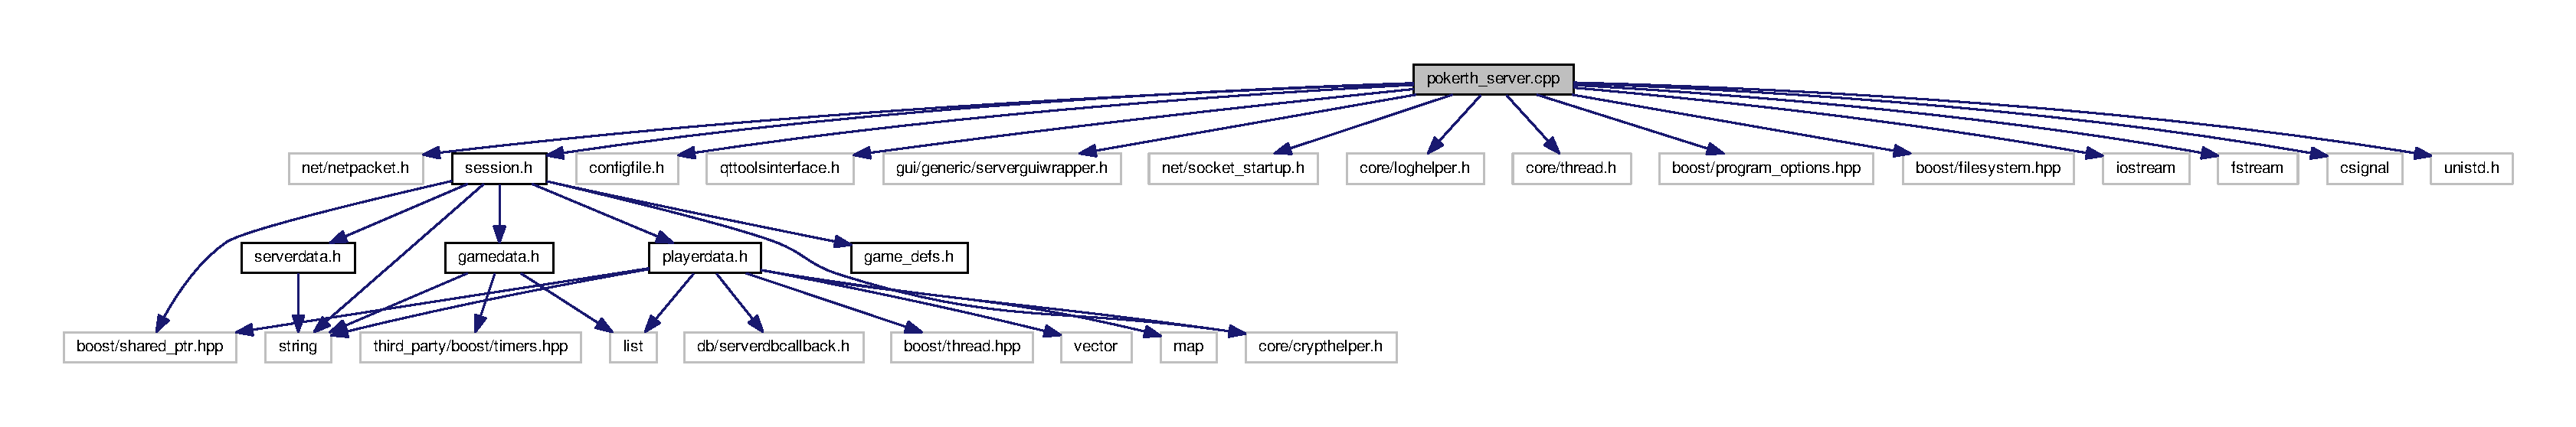
\includegraphics[width=350pt]{pokerth__server_8cpp__incl}
\end{center}
\end{figure}
\subsection*{매크로}
\begin{DoxyCompactItemize}
\item 
\#define \hyperlink{pokerth__server_8cpp_a1bdcac39cce77af91b60ca6044fae397}{E\-N\-A\-B\-L\-E\-\_\-\-L\-E\-A\-K\-\_\-\-C\-H\-E\-C\-K}()
\end{DoxyCompactItemize}
\subsection*{함수}
\begin{DoxyCompactItemize}
\item 
void \hyperlink{pokerth__server_8cpp_af14ec4e71a31fd4a83d28aa24b132090}{Terminate\-Handler} (int)
\item 
int \hyperlink{pokerth__server_8cpp_aa10914f5d815f5943722ae8be203eeff}{daemon} (int, int)
\item 
int \hyperlink{pokerth__server_8cpp_a0ddf1224851353fc92bfbff6f499fa97}{main} (int argc, char $\ast$argv\mbox{[}$\,$\mbox{]})
\end{DoxyCompactItemize}
\subsection*{변수}
\begin{DoxyCompactItemize}
\item 
volatile int \hyperlink{pokerth__server_8cpp_ac2975e1f9e3143587d34d93d980d26db}{g\-\_\-pokerth\-Terminate} = 0
\end{DoxyCompactItemize}


\subsection{매크로 문서화}
\hypertarget{pokerth__server_8cpp_a1bdcac39cce77af91b60ca6044fae397}{\index{pokerth\-\_\-server.\-cpp@{pokerth\-\_\-server.\-cpp}!E\-N\-A\-B\-L\-E\-\_\-\-L\-E\-A\-K\-\_\-\-C\-H\-E\-C\-K@{E\-N\-A\-B\-L\-E\-\_\-\-L\-E\-A\-K\-\_\-\-C\-H\-E\-C\-K}}
\index{E\-N\-A\-B\-L\-E\-\_\-\-L\-E\-A\-K\-\_\-\-C\-H\-E\-C\-K@{E\-N\-A\-B\-L\-E\-\_\-\-L\-E\-A\-K\-\_\-\-C\-H\-E\-C\-K}!pokerth_server.cpp@{pokerth\-\_\-server.\-cpp}}
\subsubsection[{E\-N\-A\-B\-L\-E\-\_\-\-L\-E\-A\-K\-\_\-\-C\-H\-E\-C\-K}]{\setlength{\rightskip}{0pt plus 5cm}\#define E\-N\-A\-B\-L\-E\-\_\-\-L\-E\-A\-K\-\_\-\-C\-H\-E\-C\-K(
\begin{DoxyParamCaption}
{}
\end{DoxyParamCaption}
)}}\label{pokerth__server_8cpp_a1bdcac39cce77af91b60ca6044fae397}


\subsection{함수 문서화}
\hypertarget{pokerth__server_8cpp_aa10914f5d815f5943722ae8be203eeff}{\index{pokerth\-\_\-server.\-cpp@{pokerth\-\_\-server.\-cpp}!daemon@{daemon}}
\index{daemon@{daemon}!pokerth_server.cpp@{pokerth\-\_\-server.\-cpp}}
\subsubsection[{daemon}]{\setlength{\rightskip}{0pt plus 5cm}int daemon (
\begin{DoxyParamCaption}
\item[{int}]{, }
\item[{int}]{}
\end{DoxyParamCaption}
)}}\label{pokerth__server_8cpp_aa10914f5d815f5943722ae8be203eeff}


이 함수를 호출하는 함수들에 대한 그래프입니다.\-:\nopagebreak
\begin{figure}[H]
\begin{center}
\leavevmode
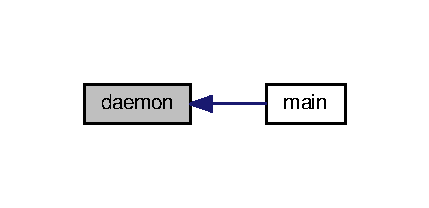
\includegraphics[width=206pt]{pokerth__server_8cpp_aa10914f5d815f5943722ae8be203eeff_icgraph}
\end{center}
\end{figure}


\hypertarget{pokerth__server_8cpp_a0ddf1224851353fc92bfbff6f499fa97}{\index{pokerth\-\_\-server.\-cpp@{pokerth\-\_\-server.\-cpp}!main@{main}}
\index{main@{main}!pokerth_server.cpp@{pokerth\-\_\-server.\-cpp}}
\subsubsection[{main}]{\setlength{\rightskip}{0pt plus 5cm}int main (
\begin{DoxyParamCaption}
\item[{int}]{argc, }
\item[{char $\ast$}]{argv\mbox{[}$\,$\mbox{]}}
\end{DoxyParamCaption}
)}}\label{pokerth__server_8cpp_a0ddf1224851353fc92bfbff6f499fa97}

\begin{DoxyCode}
89 \{
90     \hyperlink{pokerth__server_8cpp_a1bdcac39cce77af91b60ca6044fae397}{ENABLE\_LEAK\_CHECK}();
91 
92     \textcolor{comment}{//\_CrtSetBreakAlloc(10260);}
93 
94     \textcolor{keywordtype}{bool} readonlyConfig = \textcolor{keyword}{false};
95     \textcolor{keywordtype}{string} pidFile;
96     \textcolor{keywordtype}{int} logLevel = 1;
97     \{
98         \textcolor{comment}{// Check command line options.}
99         po::options\_description desc(\textcolor{stringliteral}{"Allowed options"});
100         desc.add\_options()
101         (\textcolor{stringliteral}{"help,h"}, \textcolor{stringliteral}{"produce help message"})
102         (\textcolor{stringliteral}{"version,v"}, \textcolor{stringliteral}{"print version string"})
103         (\textcolor{stringliteral}{"log-level,l"}, po::value<int>(), \textcolor{stringliteral}{"set log level (0=minimal, 1=default, 2=verbose)"})
104         (\textcolor{stringliteral}{"pid-file,p"}, po::value<string>(), \textcolor{stringliteral}{"create pid-file in different location"})
105         (\textcolor{stringliteral}{"readonly-config"}, \textcolor{stringliteral}{"treat config file as read-only"})
106         ;
107 
108         po::variables\_map vm;
109         po::store(po::parse\_command\_line(argc, argv, desc), vm);
110         po::notify(vm);
111 
112         \textcolor{keywordflow}{if} (vm.count(\textcolor{stringliteral}{"help"})) \{
113             cout << desc << endl;
114             \textcolor{keywordflow}{return} 1;
115         \}
116         \textcolor{keywordflow}{if} (vm.count(\textcolor{stringliteral}{"version"})) \{
117             cout << \textcolor{stringliteral}{"PokerTH server version   "} << \hyperlink{game__defs_8h_ac16e1f5cf0ee8fbb4b1a0cd790e5f262}{POKERTH\_BETA\_RELEASE\_STRING} <
      < endl
118                  << \textcolor{stringliteral}{"Network protocol version "} << NET\_VERSION\_MAJOR << \textcolor{stringliteral}{"."} << NET\_VERSION\_MINOR << endl;
119             \textcolor{keywordflow}{return} 1;
120         \}
121         \textcolor{keywordflow}{if} (vm.count(\textcolor{stringliteral}{"log-level"})) \{
122             logLevel = vm[\textcolor{stringliteral}{"log-level"}].as<\textcolor{keywordtype}{int}>();
123             \textcolor{keywordflow}{if} (logLevel < 0 || logLevel > 2) \{
124                 cout << \textcolor{stringliteral}{"Invalid log-level: \(\backslash\)""} << logLevel << \textcolor{stringliteral}{"\(\backslash\)", allowed range 0-2."} << endl;
125                 \textcolor{keywordflow}{return} 1;
126             \}
127         \}
128         \textcolor{keywordflow}{if} (vm.count(\textcolor{stringliteral}{"pid-file"}))
129             pidFile = vm[\textcolor{stringliteral}{"pid-file"}].as<string>();
130         \textcolor{keywordflow}{if} (vm.count(\textcolor{stringliteral}{"readonly-config"}))
131             readonlyConfig = \textcolor{keyword}{true};
132     \}
133 
134     boost::shared\_ptr<QtToolsInterface> myQtToolsInterface(CreateQtToolsWrapper());
135     \textcolor{comment}{//create defaultconfig}
136     boost::shared\_ptr<ConfigFile> myConfig(\textcolor{keyword}{new} ConfigFile(argv[0], readonlyConfig));
137     loghelper\_init(myQtToolsInterface->stringFromUtf8(myConfig->readConfigString(\textcolor{stringliteral}{"LogDir"})), logLevel);
138 
139     \textcolor{comment}{// TODO: Hack}
140 \textcolor{preprocessor}{#ifndef \_WIN32
}
141 \textcolor{preprocessor}{}\textcolor{preprocessor}{#ifdef QT\_NO\_DEBUG
}
142 \textcolor{preprocessor}{}    \textcolor{keywordflow}{if} (\hyperlink{pokerth__server_8cpp_aa10914f5d815f5943722ae8be203eeff}{daemon}(0, 0) != 0) \{
143         cout << \textcolor{stringliteral}{"Failed to start daemon."} << endl;
144         \textcolor{keywordflow}{return} 1;
145     \}
146 \textcolor{preprocessor}{#endif
}
147 \textcolor{preprocessor}{}\textcolor{preprocessor}{#endif
}
148 \textcolor{preprocessor}{}
149     signal(SIGTERM, \hyperlink{pokerth__server_8cpp_af14ec4e71a31fd4a83d28aa24b132090}{TerminateHandler});
150     signal(SIGINT, \hyperlink{pokerth__server_8cpp_af14ec4e71a31fd4a83d28aa24b132090}{TerminateHandler});
151 
152     socket\_startup();
153 
154     LOG\_MSG(\textcolor{stringliteral}{"Starting PokerTH dedicated server. Availability: IPv6 "}
155             << socket\_has\_ipv6() << \textcolor{stringliteral}{", SCTP "} << socket\_has\_sctp() << \textcolor{stringliteral}{", Dual Stack "} << 
      socket\_has\_dual\_stack() << \textcolor{stringliteral}{"."});
156 
157     \textcolor{comment}{// Store pid in file.}
158     \textcolor{keywordflow}{if} (pidFile.empty()) \{
159         path tmpPidPath(myConfig->readConfigString(\textcolor{stringliteral}{"LogDir"}));
160         tmpPidPath /= \textcolor{stringliteral}{"pokerth.pid"};
161         pidFile = tmpPidPath.directory\_string();
162     \}
163     \{
164         std::ofstream pidStream(pidFile.c\_str(), ios\_base::out | ios\_base::trunc);
165         \textcolor{keywordflow}{if} (!pidStream.fail())
166             pidStream << getpid();
167         \textcolor{keywordflow}{else}
168             LOG\_ERROR(\textcolor{stringliteral}{"Could not create process id file \(\backslash\)""} << pidFile << \textcolor{stringliteral}{"\(\backslash\)"!"});
169     \}
170 
171     \textcolor{comment}{// Create pseudo Gui Wrapper for the server.}
172     boost::shared\_ptr<GuiInterface> myServerGuiInterface(\textcolor{keyword}{new} ServerGuiWrapper(myConfig.get(), NULL, NULL, 
      NULL));
173     boost::shared\_ptr<Session> session(\textcolor{keyword}{new} \hyperlink{class_session}{Session}(myServerGuiInterface.get(), myConfig.get(), NULL)
      );
174     \textcolor{keywordflow}{if} (!session->init())
175         LOG\_ERROR(\textcolor{stringliteral}{"Missing files - please check your directory settings!"});
176     myServerGuiInterface->setSession(session);
177 
178     myServerGuiInterface->getSession()->startNetworkServer(\textcolor{keyword}{true});
179     \textcolor{keywordflow}{while} (!\hyperlink{pokerth__server_8cpp_ac2975e1f9e3143587d34d93d980d26db}{g\_pokerthTerminate}) \{
180         Thread::Msleep(100);
181         \textcolor{keywordflow}{if} (myServerGuiInterface->getSession()->pollNetworkServerTerminated())
182             \hyperlink{pokerth__server_8cpp_ac2975e1f9e3143587d34d93d980d26db}{g\_pokerthTerminate} = \textcolor{keyword}{true};
183     \}
184     myServerGuiInterface->getSession()->terminateNetworkServer();
185     session.reset();
186     myServerGuiInterface.reset();
187     myConfig.reset();
188 
189     LOG\_MSG(\textcolor{stringliteral}{"Terminating PokerTH dedicated server."} << endl);
190     socket\_cleanup();
191     \textcolor{keywordflow}{return} 0;
192 \}\end{DoxyCode}


이 함수 내부에서 호출하는 함수들에 대한 그래프입니다.\-:\nopagebreak
\begin{figure}[H]
\begin{center}
\leavevmode
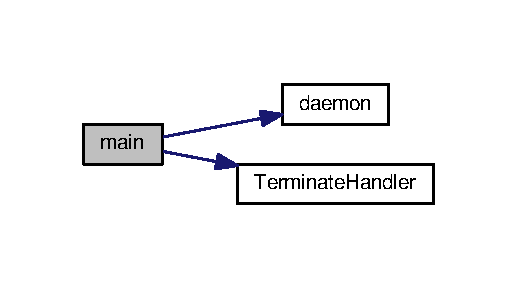
\includegraphics[width=248pt]{pokerth__server_8cpp_a0ddf1224851353fc92bfbff6f499fa97_cgraph}
\end{center}
\end{figure}


\hypertarget{pokerth__server_8cpp_af14ec4e71a31fd4a83d28aa24b132090}{\index{pokerth\-\_\-server.\-cpp@{pokerth\-\_\-server.\-cpp}!Terminate\-Handler@{Terminate\-Handler}}
\index{Terminate\-Handler@{Terminate\-Handler}!pokerth_server.cpp@{pokerth\-\_\-server.\-cpp}}
\subsubsection[{Terminate\-Handler}]{\setlength{\rightskip}{0pt plus 5cm}void Terminate\-Handler (
\begin{DoxyParamCaption}
\item[{int}]{}
\end{DoxyParamCaption}
)}}\label{pokerth__server_8cpp_af14ec4e71a31fd4a83d28aa24b132090}

\begin{DoxyCode}
73 \{
74     \hyperlink{pokerth__server_8cpp_ac2975e1f9e3143587d34d93d980d26db}{g\_pokerthTerminate} = 1;
75 \}
\end{DoxyCode}


이 함수를 호출하는 함수들에 대한 그래프입니다.\-:\nopagebreak
\begin{figure}[H]
\begin{center}
\leavevmode
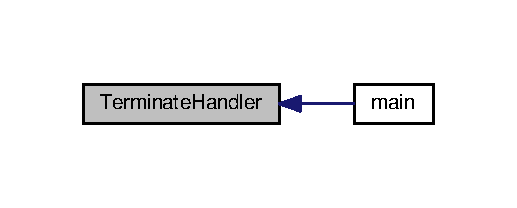
\includegraphics[width=248pt]{pokerth__server_8cpp_af14ec4e71a31fd4a83d28aa24b132090_icgraph}
\end{center}
\end{figure}




\subsection{변수 문서화}
\hypertarget{pokerth__server_8cpp_ac2975e1f9e3143587d34d93d980d26db}{\index{pokerth\-\_\-server.\-cpp@{pokerth\-\_\-server.\-cpp}!g\-\_\-pokerth\-Terminate@{g\-\_\-pokerth\-Terminate}}
\index{g\-\_\-pokerth\-Terminate@{g\-\_\-pokerth\-Terminate}!pokerth_server.cpp@{pokerth\-\_\-server.\-cpp}}
\subsubsection[{g\-\_\-pokerth\-Terminate}]{\setlength{\rightskip}{0pt plus 5cm}volatile int g\-\_\-pokerth\-Terminate = 0}}\label{pokerth__server_8cpp_ac2975e1f9e3143587d34d93d980d26db}

\hypertarget{serverdata_8h}{\section{serverdata.\-h 파일 참조}
\label{serverdata_8h}\index{serverdata.\-h@{serverdata.\-h}}
}
{\ttfamily \#include $<$string$>$}\\*
serverdata.\-h에 대한 include 의존 그래프\nopagebreak
\begin{figure}[H]
\begin{center}
\leavevmode
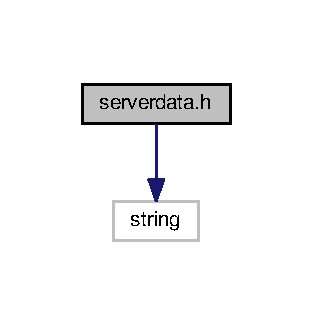
\includegraphics[width=150pt]{serverdata_8h__incl}
\end{center}
\end{figure}
이 그래프는 이 파일을 직/간접적으로 include 하는 파일들을 보여줍니다.\-:\nopagebreak
\begin{figure}[H]
\begin{center}
\leavevmode
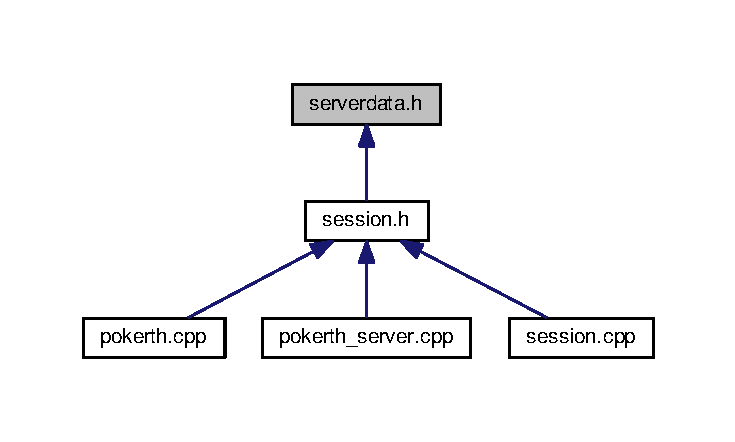
\includegraphics[width=350pt]{serverdata_8h__dep__incl}
\end{center}
\end{figure}
\subsection*{클래스}
\begin{DoxyCompactItemize}
\item 
struct \hyperlink{struct_server_info}{Server\-Info}
\item 
struct \hyperlink{struct_server_stats}{Server\-Stats}
\end{DoxyCompactItemize}

\hypertarget{session_8cpp}{\section{session.\-cpp 파일 참조}
\label{session_8cpp}\index{session.\-cpp@{session.\-cpp}}
}
{\ttfamily \#include $<$boost/asio.\-hpp$>$}\\*
{\ttfamily \#include $<$net/socket\-\_\-helper.\-h$>$}\\*
{\ttfamily \#include \char`\"{}session.\-h\char`\"{}}\\*
{\ttfamily \#include \char`\"{}game.\-h\char`\"{}}\\*
{\ttfamily \#include \char`\"{}log.\-h\char`\"{}}\\*
{\ttfamily \#include \char`\"{}guiinterface.\-h\char`\"{}}\\*
{\ttfamily \#include \char`\"{}configfile.\-h\char`\"{}}\\*
{\ttfamily \#include $<$qttoolsinterface.\-h$>$}\\*
{\ttfamily \#include $<$localenginefactory.\-h$>$}\\*
{\ttfamily \#include $<$clientenginefactory.\-h$>$}\\*
{\ttfamily \#include $<$net/clientthread.\-h$>$}\\*
{\ttfamily \#include $<$core/avatarmanager.\-h$>$}\\*
{\ttfamily \#include $<$net/servermanagerfactory.\-h$>$}\\*
{\ttfamily \#include $<$sstream$>$}\\*
session.\-cpp에 대한 include 의존 그래프\nopagebreak
\begin{figure}[H]
\begin{center}
\leavevmode
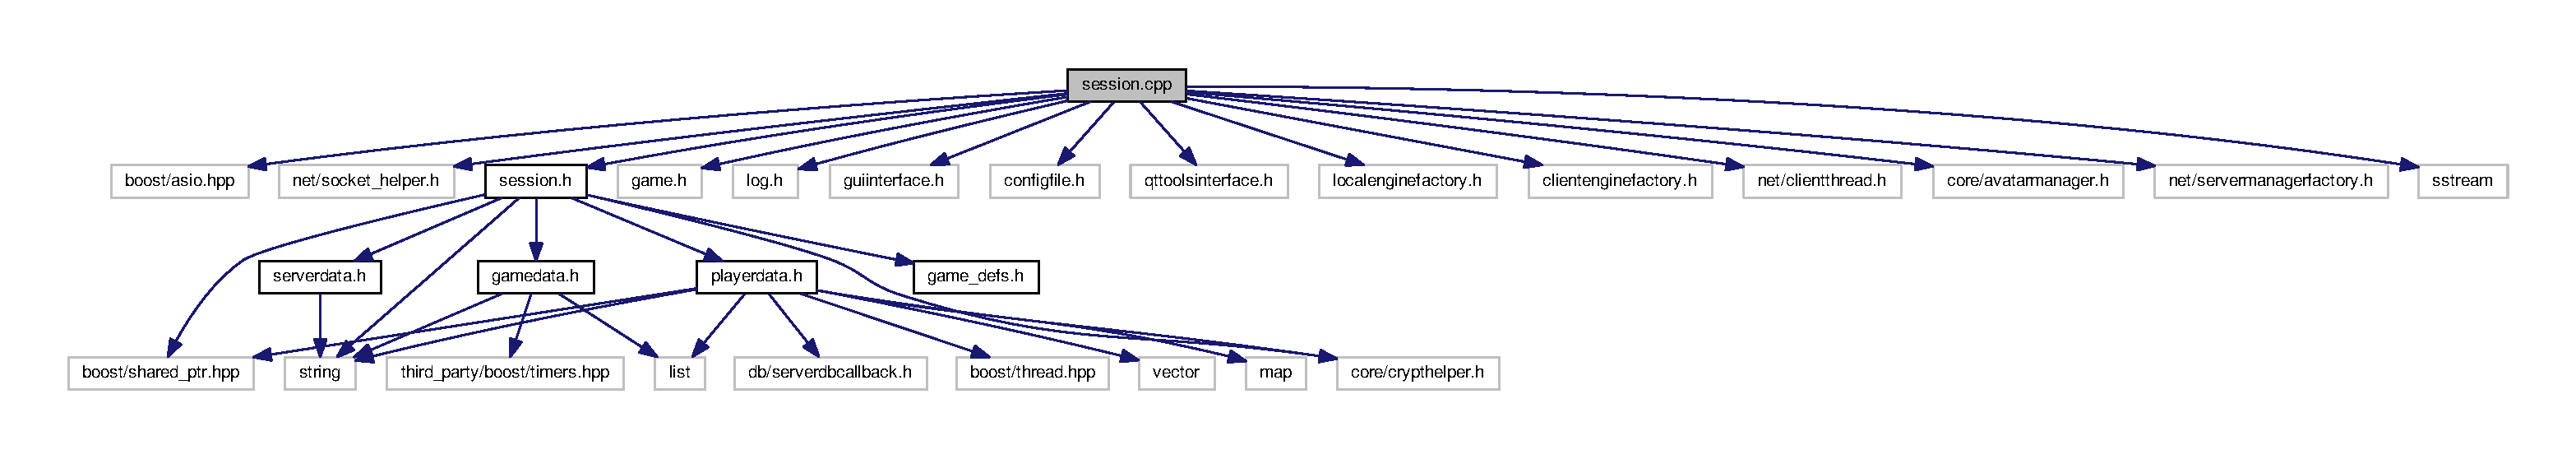
\includegraphics[width=350pt]{session_8cpp__incl}
\end{center}
\end{figure}
\subsection*{매크로}
\begin{DoxyCompactItemize}
\item 
\#define \hyperlink{session_8cpp_ac4cfb210528149df9891fb4c5529a366}{N\-E\-T\-\_\-\-C\-L\-I\-E\-N\-T\-\_\-\-T\-E\-R\-M\-I\-N\-A\-T\-E\-\_\-\-T\-I\-M\-E\-O\-U\-T\-\_\-\-M\-S\-E\-C}~2000
\item 
\#define \hyperlink{session_8cpp_a09aa3eef2094a49576365bb7715715c3}{N\-E\-T\-\_\-\-I\-R\-C\-\_\-\-T\-E\-R\-M\-I\-N\-A\-T\-E\-\_\-\-T\-I\-M\-E\-O\-U\-T\-\_\-\-M\-S\-E\-C}~2000
\item 
\#define \hyperlink{session_8cpp_ae40f8ea78cc800300b894fc55d38c146}{N\-E\-T\-\_\-\-D\-E\-F\-A\-U\-L\-T\-\_\-\-G\-A\-M\-E}~\char`\"{}default\char`\"{}
\end{DoxyCompactItemize}


\subsection{매크로 문서화}
\hypertarget{session_8cpp_ac4cfb210528149df9891fb4c5529a366}{\index{session.\-cpp@{session.\-cpp}!N\-E\-T\-\_\-\-C\-L\-I\-E\-N\-T\-\_\-\-T\-E\-R\-M\-I\-N\-A\-T\-E\-\_\-\-T\-I\-M\-E\-O\-U\-T\-\_\-\-M\-S\-E\-C@{N\-E\-T\-\_\-\-C\-L\-I\-E\-N\-T\-\_\-\-T\-E\-R\-M\-I\-N\-A\-T\-E\-\_\-\-T\-I\-M\-E\-O\-U\-T\-\_\-\-M\-S\-E\-C}}
\index{N\-E\-T\-\_\-\-C\-L\-I\-E\-N\-T\-\_\-\-T\-E\-R\-M\-I\-N\-A\-T\-E\-\_\-\-T\-I\-M\-E\-O\-U\-T\-\_\-\-M\-S\-E\-C@{N\-E\-T\-\_\-\-C\-L\-I\-E\-N\-T\-\_\-\-T\-E\-R\-M\-I\-N\-A\-T\-E\-\_\-\-T\-I\-M\-E\-O\-U\-T\-\_\-\-M\-S\-E\-C}!session.cpp@{session.\-cpp}}
\subsubsection[{N\-E\-T\-\_\-\-C\-L\-I\-E\-N\-T\-\_\-\-T\-E\-R\-M\-I\-N\-A\-T\-E\-\_\-\-T\-I\-M\-E\-O\-U\-T\-\_\-\-M\-S\-E\-C}]{\setlength{\rightskip}{0pt plus 5cm}\#define N\-E\-T\-\_\-\-C\-L\-I\-E\-N\-T\-\_\-\-T\-E\-R\-M\-I\-N\-A\-T\-E\-\_\-\-T\-I\-M\-E\-O\-U\-T\-\_\-\-M\-S\-E\-C~2000}}\label{session_8cpp_ac4cfb210528149df9891fb4c5529a366}
\hypertarget{session_8cpp_ae40f8ea78cc800300b894fc55d38c146}{\index{session.\-cpp@{session.\-cpp}!N\-E\-T\-\_\-\-D\-E\-F\-A\-U\-L\-T\-\_\-\-G\-A\-M\-E@{N\-E\-T\-\_\-\-D\-E\-F\-A\-U\-L\-T\-\_\-\-G\-A\-M\-E}}
\index{N\-E\-T\-\_\-\-D\-E\-F\-A\-U\-L\-T\-\_\-\-G\-A\-M\-E@{N\-E\-T\-\_\-\-D\-E\-F\-A\-U\-L\-T\-\_\-\-G\-A\-M\-E}!session.cpp@{session.\-cpp}}
\subsubsection[{N\-E\-T\-\_\-\-D\-E\-F\-A\-U\-L\-T\-\_\-\-G\-A\-M\-E}]{\setlength{\rightskip}{0pt plus 5cm}\#define N\-E\-T\-\_\-\-D\-E\-F\-A\-U\-L\-T\-\_\-\-G\-A\-M\-E~\char`\"{}default\char`\"{}}}\label{session_8cpp_ae40f8ea78cc800300b894fc55d38c146}
\hypertarget{session_8cpp_a09aa3eef2094a49576365bb7715715c3}{\index{session.\-cpp@{session.\-cpp}!N\-E\-T\-\_\-\-I\-R\-C\-\_\-\-T\-E\-R\-M\-I\-N\-A\-T\-E\-\_\-\-T\-I\-M\-E\-O\-U\-T\-\_\-\-M\-S\-E\-C@{N\-E\-T\-\_\-\-I\-R\-C\-\_\-\-T\-E\-R\-M\-I\-N\-A\-T\-E\-\_\-\-T\-I\-M\-E\-O\-U\-T\-\_\-\-M\-S\-E\-C}}
\index{N\-E\-T\-\_\-\-I\-R\-C\-\_\-\-T\-E\-R\-M\-I\-N\-A\-T\-E\-\_\-\-T\-I\-M\-E\-O\-U\-T\-\_\-\-M\-S\-E\-C@{N\-E\-T\-\_\-\-I\-R\-C\-\_\-\-T\-E\-R\-M\-I\-N\-A\-T\-E\-\_\-\-T\-I\-M\-E\-O\-U\-T\-\_\-\-M\-S\-E\-C}!session.cpp@{session.\-cpp}}
\subsubsection[{N\-E\-T\-\_\-\-I\-R\-C\-\_\-\-T\-E\-R\-M\-I\-N\-A\-T\-E\-\_\-\-T\-I\-M\-E\-O\-U\-T\-\_\-\-M\-S\-E\-C}]{\setlength{\rightskip}{0pt plus 5cm}\#define N\-E\-T\-\_\-\-I\-R\-C\-\_\-\-T\-E\-R\-M\-I\-N\-A\-T\-E\-\_\-\-T\-I\-M\-E\-O\-U\-T\-\_\-\-M\-S\-E\-C~2000}}\label{session_8cpp_a09aa3eef2094a49576365bb7715715c3}

\hypertarget{session_8h}{\section{session.\-h 파일 참조}
\label{session_8h}\index{session.\-h@{session.\-h}}
}
{\ttfamily \#include $<$boost/shared\-\_\-ptr.\-hpp$>$}\\*
{\ttfamily \#include $<$string$>$}\\*
{\ttfamily \#include \char`\"{}serverdata.\-h\char`\"{}}\\*
{\ttfamily \#include \char`\"{}gamedata.\-h\char`\"{}}\\*
{\ttfamily \#include \char`\"{}playerdata.\-h\char`\"{}}\\*
{\ttfamily \#include \char`\"{}game\-\_\-defs.\-h\char`\"{}}\\*
{\ttfamily \#include $<$core/crypthelper.\-h$>$}\\*
session.\-h에 대한 include 의존 그래프\nopagebreak
\begin{figure}[H]
\begin{center}
\leavevmode
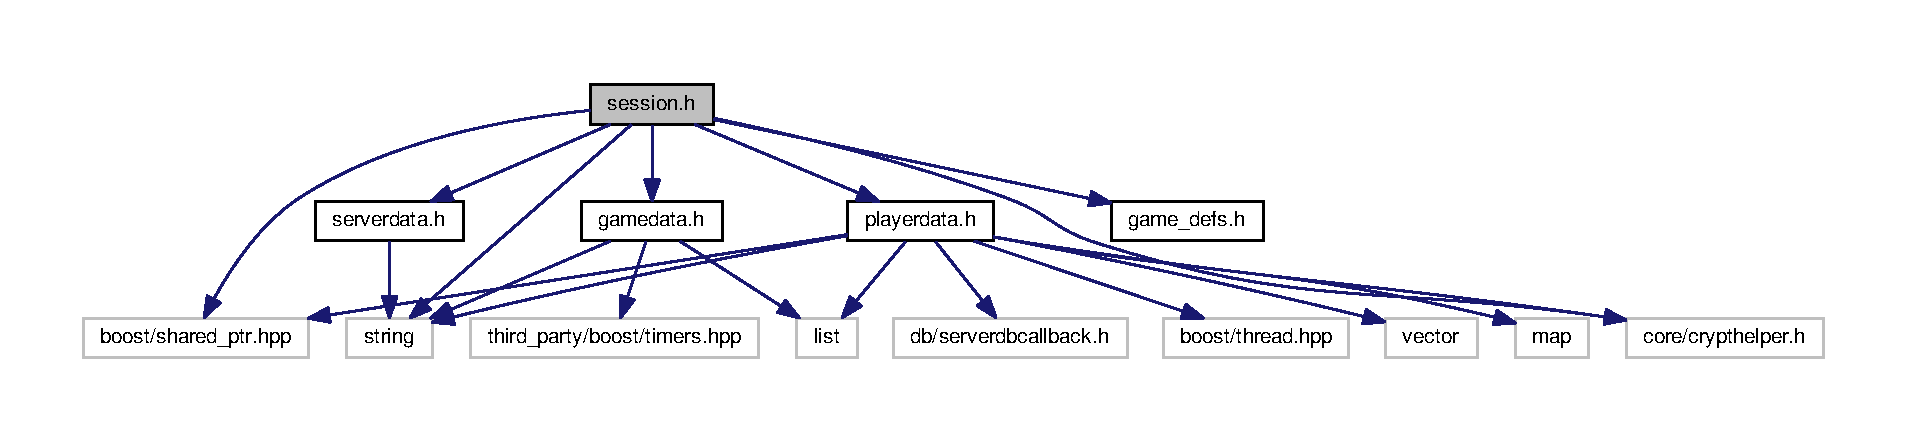
\includegraphics[width=350pt]{session_8h__incl}
\end{center}
\end{figure}
이 그래프는 이 파일을 직/간접적으로 include 하는 파일들을 보여줍니다.\-:\nopagebreak
\begin{figure}[H]
\begin{center}
\leavevmode
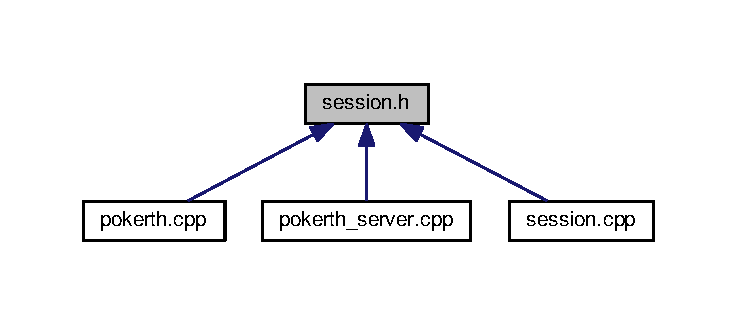
\includegraphics[width=350pt]{session_8h__dep__incl}
\end{center}
\end{figure}
\subsection*{클래스}
\begin{DoxyCompactItemize}
\item 
class \hyperlink{class_session}{Session}
\end{DoxyCompactItemize}

\hypertarget{zlib__compress_8cpp}{\section{zlib\-\_\-compress.\-cpp 파일 참조}
\label{zlib__compress_8cpp}\index{zlib\-\_\-compress.\-cpp@{zlib\-\_\-compress.\-cpp}}
}
{\ttfamily \#include $<$boost/filesystem.\-hpp$>$}\\*
{\ttfamily \#include $<$boost/iostreams/filtering\-\_\-streambuf.\-hpp$>$}\\*
{\ttfamily \#include $<$boost/iostreams/copy.\-hpp$>$}\\*
{\ttfamily \#include $<$boost/iostreams/filter/zlib.\-hpp$>$}\\*
{\ttfamily \#include $<$iostream$>$}\\*
{\ttfamily \#include $<$fstream$>$}\\*
{\ttfamily \#include $<$string$>$}\\*
zlib\-\_\-compress.\-cpp에 대한 include 의존 그래프\nopagebreak
\begin{figure}[H]
\begin{center}
\leavevmode
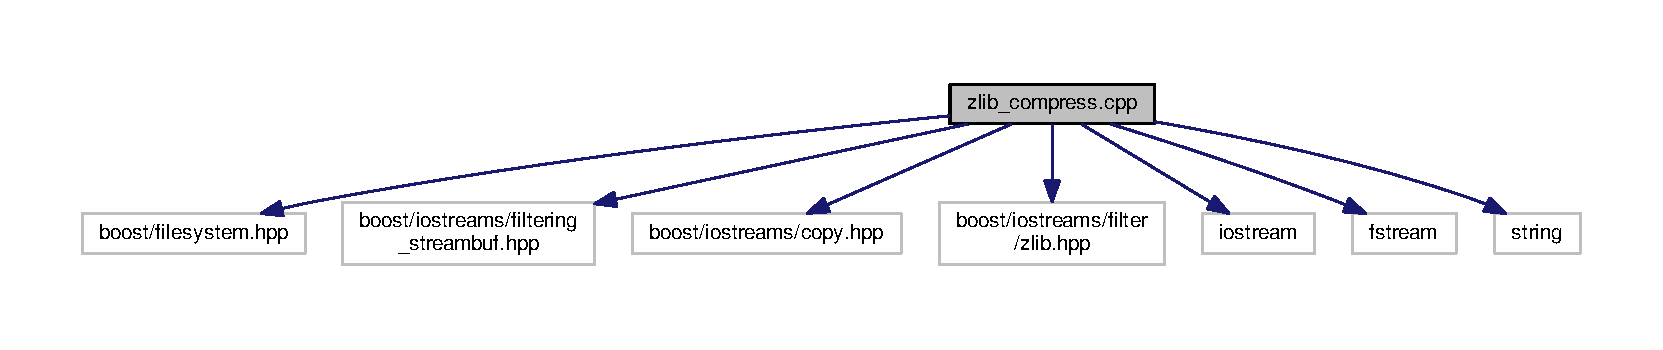
\includegraphics[width=350pt]{zlib__compress_8cpp__incl}
\end{center}
\end{figure}
\subsection*{함수}
\begin{DoxyCompactItemize}
\item 
int \hyperlink{zlib__compress_8cpp_a0ddf1224851353fc92bfbff6f499fa97}{main} (int argc, char $\ast$argv\mbox{[}$\,$\mbox{]})
\end{DoxyCompactItemize}


\subsection{함수 문서화}
\hypertarget{zlib__compress_8cpp_a0ddf1224851353fc92bfbff6f499fa97}{\index{zlib\-\_\-compress.\-cpp@{zlib\-\_\-compress.\-cpp}!main@{main}}
\index{main@{main}!zlib_compress.cpp@{zlib\-\_\-compress.\-cpp}}
\subsubsection[{main}]{\setlength{\rightskip}{0pt plus 5cm}int main (
\begin{DoxyParamCaption}
\item[{int}]{argc, }
\item[{char $\ast$}]{argv\mbox{[}$\,$\mbox{]}}
\end{DoxyParamCaption}
)}}\label{zlib__compress_8cpp_a0ddf1224851353fc92bfbff6f499fa97}

\begin{DoxyCode}
47 \{
48     \textcolor{keywordflow}{if} (argc != 2) \{
49         cout << \textcolor{stringliteral}{"Usage: zlib\_compress <text input file>"} << endl;
50         \textcolor{keywordflow}{return} 1;
51     \}
52     \textcolor{comment}{// Use input file name, and write to input file with additional ".z".}
53     path inputFilePath(argv[1]);
54     path outputFilePath(inputFilePath);
55     outputFilePath = change\_extension(outputFilePath, extension(outputFilePath) + \textcolor{stringliteral}{".z"});
56     \textcolor{comment}{// Check whether file exists.}
57     \textcolor{keywordflow}{if} (!exists(inputFilePath)) \{
58         cerr << \textcolor{stringliteral}{"Input file does not exist."} << endl;
59         \textcolor{keywordflow}{return} 2;
60     \}
61     \textcolor{keywordflow}{try} \{
62         std::ifstream inFile(inputFilePath.directory\_string().c\_str(), ios\_base::in);
63         std::ofstream outFile(outputFilePath.directory\_string().c\_str(), ios\_base::out | ios\_base::binary);
64         boost::iostreams::filtering\_streambuf<boost::iostreams::output> out;
65         out.push(boost::iostreams::zlib\_compressor());
66         out.push(outFile);
67         boost::iostreams::copy(inFile, out);
68         cout << \textcolor{stringliteral}{"Compression of \(\backslash\)""} << inputFilePath.directory\_string() << \textcolor{stringliteral}{"\(\backslash\)" to \(\backslash\)""} << outputFilePath.
      directory\_string() << \textcolor{stringliteral}{"\(\backslash\)" was successful."} << endl;
69     \} \textcolor{keywordflow}{catch} (...) \{
70         cerr << \textcolor{stringliteral}{"Compression failed."} << endl;
71         \textcolor{keywordflow}{return} 3;
72     \}
73 
74     \textcolor{keywordflow}{return} 0;
75 \}
\end{DoxyCode}

%--- End generated contents ---

% Index
\newpage
\phantomsection
\addcontentsline{toc}{chapter}{색인}
\printindex

\end{document}
